\documentclass[a4paper,twoside,12pt]{report}
\usepackage[pdftex]{graphicx}
\usepackage{tocloft}
%
\usepackage[smaller]{acronym}
\usepackage{amsfonts}
\usepackage{amsmath}
\usepackage{atlasphysics}
\usepackage{bbold}
\usepackage{lscape}
\usepackage{booktabs}
\usepackage[pdftex,color]{changebar}
\usepackage{fancyhdr}
\usepackage{hyperref}
\usepackage{lineno}
\usepackage{mathrsfs}
\usepackage{multirow}
\usepackage{pdfpages}
\usepackage{sectsty}
\usepackage{setspace}
\usepackage{subfig}
\usepackage{type1cm}
\usepackage[normalem]{ulem}
\usepackage{url}
\usepackage{xspace}
\usepackage{upgreek}
\usepackage{ifthen}
\newboolean{uprightparticles}
\setboolean{uprightparticles}{false}
\usepackage[Sonny]{fncychap} %Styles: Sonny, Lenny, Glenn, Conny, Rejne, Bjarne, and Bjornstrup.

%%% $Id: lhcb-symbols-def.tex 58560 2014-07-29 10:44:38Z pluca $
%%% ======================================================================
%%% Purpose: Standard LHCb aliases
%%% Author: Originally Ulrik Egede, adapted by Tomasz Skwarnicki for templates,
%%% rewritten by Chris Parkes
%%% Maintainer : Ulrik Egede (2010 - 2012)
%%% =======================================================================

%%% To use this file outside the normal LHCb document environment, the
%%% following should be added in a preamble (before \begin{document}
%%%
%%%\usepackage{ifthen} 
%%%\newboolean{uprightparticles}
%%%\setboolean{uprightparticles}{false} %Set true for upright particle symbols
%%% \usepackage{xspace} 
%%% \usepackage{upgreek}

%%%%%%%%%%%%%%%%%%%%%%%%%%%%%%%%%%%%%%%%%%%%%%%%%%%%%%%%%%%%
%%%
%%% The following is to ensure that the template automatically can process
%%% this file.
%%%
%%% Add comments with at least three %%% preceding.
%%% Add new sections with one % preceding
%%% Add new subsections with two %% preceding
%%%%%%%%%%%%%%%%%%%%%%%%%%%%%%%%%%%%%%%%%%%%%%%%%%%%%%%%%%%%

%%%%%%%%%%%%%
% Experiments
%%%%%%%%%%%%%
\def\lhcb {\mbox{LHCb}\xspace}
\def\atlas  {\mbox{ATLAS}\xspace}
\def\cms    {\mbox{CMS}\xspace}
\def\alice  {\mbox{ALICE}\xspace}
\def\babar  {\mbox{BaBar}\xspace}
\def\belle  {\mbox{Belle}\xspace}
\def\cleo   {\mbox{CLEO}\xspace}
\def\cdf    {\mbox{CDF}\xspace}
\def\dzero  {\mbox{D0}\xspace}
\def\aleph  {\mbox{ALEPH}\xspace}
\def\delphi {\mbox{DELPHI}\xspace}
\def\opal   {\mbox{OPAL}\xspace}
\def\lthree {\mbox{L3}\xspace}
\def\sld    {\mbox{SLD}\xspace}
%%%\def\argus  {\mbox{ARGUS}\xspace}
%%%\def\uaone  {\mbox{UA1}\xspace}
%%%\def\uatwo  {\mbox{UA2}\xspace}
%%%\def\ux85 {\mbox{UX85}\xspace}
\def\cern {\mbox{CERN}\xspace}
\def\lhc    {\mbox{LHC}\xspace}
\def\lep    {\mbox{LEP}\xspace}
\def\tevatron {Tevatron\xspace}

%% LHCb sub-detectors and sub-systems

%%%\def\pu     {PU\xspace}
\def\velo   {VELO\xspace}
\def\rich   {RICH\xspace}
\def\richone {RICH1\xspace}
\def\richtwo {RICH2\xspace}
\def\ttracker {TT\xspace}
\def\intr   {IT\xspace}
\def\st     {ST\xspace}
\def\ot     {OT\xspace}
%%%\def\Tone   {T1\xspace}
%%%\def\Ttwo   {T2\xspace}
%%%\def\Tthree {T3\xspace}
%%%\def\Mone   {M1\xspace}
%%%\def\Mtwo   {M2\xspace}
%%%\def\Mthree {M3\xspace}
%%%\def\Mfour  {M4\xspace}
%%%\def\Mfive  {M5\xspace}
\def\spd    {SPD\xspace}
\def\presh  {PS\xspace}
\def\ecal   {ECAL\xspace}
\def\hcal   {HCAL\xspace}
%%%\def\bcm    {BCM\xspace}

%%%\def\ode    {ODE\xspace}
%%%\def\daq    {DAQ\xspace}
%%%\def\tfc    {TFC\xspace}
%%%\def\ecs    {ECS\xspace}
%%%\def\lone   {L0\xspace}
%%%\def\hlt    {HLT\xspace}
%%%\def\hltone {HLT1\xspace}
%%%\def\hlttwo {HLT2\xspace}

%%% Upright (not slanted) Particles

\ifthenelse{\boolean{uprightparticles}}%
{\def\Palpha      {\ensuremath{\upalpha}\xspace}
 \def\Pbeta       {\ensuremath{\upbeta}\xspace}
 \def\Pgamma      {\ensuremath{\upgamma}\xspace}                 
 \def\Pdelta      {\ensuremath{\updelta}\xspace}                 
 \def\Pepsilon    {\ensuremath{\upepsilon}\xspace}                 
 \def\Pvarepsilon {\ensuremath{\upvarepsilon}\xspace}                 
 \def\Pzeta       {\ensuremath{\upzeta}\xspace}                 
 \def\Peta        {\ensuremath{\upeta}\xspace}                 
 \def\Ptheta      {\ensuremath{\uptheta}\xspace}                 
 \def\Pvartheta   {\ensuremath{\upvartheta}\xspace}                 
 \def\Piota       {\ensuremath{\upiota}\xspace}                 
 \def\Pkappa      {\ensuremath{\upkappa}\xspace}                 
 \def\Plambda     {\ensuremath{\uplambda}\xspace}                 
 \def\Pmu         {\ensuremath{\upmu}\xspace}                 
 \def\Pnu         {\ensuremath{\upnu}\xspace}                 
 \def\Pxi         {\ensuremath{\upxi}\xspace}                 
 \def\Ppi         {\ensuremath{\uppi}\xspace}                 
 \def\Pvarpi      {\ensuremath{\upvarpi}\xspace}                 
 \def\Prho        {\ensuremath{\uprho}\xspace}                 
 \def\Pvarrho     {\ensuremath{\upvarrho}\xspace}                 
 \def\Ptau        {\ensuremath{\uptau}\xspace}                 
 \def\Pupsilon    {\ensuremath{\upupsilon}\xspace}                 
 \def\Pphi        {\ensuremath{\upphi}\xspace}                 
 \def\Pvarphi     {\ensuremath{\upvarphi}\xspace}                 
 \def\Pchi        {\ensuremath{\upchi}\xspace}                 
 \def\Ppsi        {\ensuremath{\uppsi}\xspace}                 
 \def\Pomega      {\ensuremath{\upomega}\xspace}                 

 \def\PDelta      {\ensuremath{\Delta}\xspace}                 
 \def\PXi      {\ensuremath{\Xi}\xspace}                 
 \def\PLambda      {\ensuremath{\Lambda}\xspace}                 
 \def\PSigma      {\ensuremath{\Sigma}\xspace}                 
 \def\POmega      {\ensuremath{\Omega}\xspace}                 
 \def\PUpsilon      {\ensuremath{\Upsilon}\xspace}                 
 
 %\mathchardef\Deltares="7101
 %\mathchardef\Xi="7104
 %\mathchardef\Lambda="7103
 %\mathchardef\Sigma="7106
 %\mathchardef\Omega="710A


 \def\PA      {\ensuremath{\mathrm{A}}\xspace}                 
 \def\PB      {\ensuremath{\mathrm{B}}\xspace}                 
 \def\PC      {\ensuremath{\mathrm{C}}\xspace}                 
 \def\PD      {\ensuremath{\mathrm{D}}\xspace}                 
 \def\PE      {\ensuremath{\mathrm{E}}\xspace}                 
 \def\PF      {\ensuremath{\mathrm{F}}\xspace}                 
 \def\PG      {\ensuremath{\mathrm{G}}\xspace}                 
 \def\PH      {\ensuremath{\mathrm{H}}\xspace}                 
 \def\PI      {\ensuremath{\mathrm{I}}\xspace}                 
 \def\PJ      {\ensuremath{\mathrm{J}}\xspace}                 
 \def\PK      {\ensuremath{\mathrm{K}}\xspace}                 
 \def\PL      {\ensuremath{\mathrm{L}}\xspace}                 
 \def\PM      {\ensuremath{\mathrm{M}}\xspace}                 
 \def\PN      {\ensuremath{\mathrm{N}}\xspace}                 
 \def\PO      {\ensuremath{\mathrm{O}}\xspace}                 
 \def\PP      {\ensuremath{\mathrm{P}}\xspace}                 
 \def\PQ      {\ensuremath{\mathrm{Q}}\xspace}                 
 \def\PR      {\ensuremath{\mathrm{R}}\xspace}                 
 \def\PS      {\ensuremath{\mathrm{S}}\xspace}                 
 \def\PT      {\ensuremath{\mathrm{T}}\xspace}                 
 \def\PU      {\ensuremath{\mathrm{U}}\xspace}                 
 \def\PV      {\ensuremath{\mathrm{V}}\xspace}                 
 \def\PW      {\ensuremath{\mathrm{W}}\xspace}                 
 \def\PX      {\ensuremath{\mathrm{X}}\xspace}                 
 \def\PY      {\ensuremath{\mathrm{Y}}\xspace}                 
 \def\PZ      {\ensuremath{\mathrm{Z}}\xspace}                 
 \def\Pa      {\ensuremath{\mathrm{a}}\xspace}                 
 \def\Pb      {\ensuremath{\mathrm{b}}\xspace}                 
 \def\Pc      {\ensuremath{\mathrm{c}}\xspace}                 
 \def\Pd      {\ensuremath{\mathrm{d}}\xspace}                 
 \def\Pe      {\ensuremath{\mathrm{e}}\xspace}                 
 \def\Pf      {\ensuremath{\mathrm{f}}\xspace}                 
 \def\Pg      {\ensuremath{\mathrm{g}}\xspace}                 
 \def\Ph      {\ensuremath{\mathrm{h}}\xspace}                 
 \def\Pi      {\ensuremath{\mathrm{i}}\xspace}                 
 \def\Pj      {\ensuremath{\mathrm{j}}\xspace}                 
 \def\Pk      {\ensuremath{\mathrm{k}}\xspace}                 
 \def\Pl      {\ensuremath{\mathrm{l}}\xspace}                 
 \def\Pm      {\ensuremath{\mathrm{m}}\xspace}                 
 \def\Pn      {\ensuremath{\mathrm{n}}\xspace}                 
 \def\Po      {\ensuremath{\mathrm{o}}\xspace}                 
 \def\Pp      {\ensuremath{\mathrm{p}}\xspace}                 
 \def\Pq      {\ensuremath{\mathrm{q}}\xspace}                 
 \def\Pr      {\ensuremath{\mathrm{r}}\xspace}                 
 \def\Ps      {\ensuremath{\mathrm{s}}\xspace}                 
 \def\Pt      {\ensuremath{\mathrm{t}}\xspace}                 
 \def\Pu      {\ensuremath{\mathrm{u}}\xspace}                 
 \def\Pv      {\ensuremath{\mathrm{v}}\xspace}                 
 \def\Pw      {\ensuremath{\mathrm{w}}\xspace}                 
 \def\Px      {\ensuremath{\mathrm{x}}\xspace}                 
 \def\Py      {\ensuremath{\mathrm{y}}\xspace}                 
 \def\Pz      {\ensuremath{\mathrm{z}}\xspace}                 
}
{\def\Palpha      {\ensuremath{\alpha}\xspace}
 \def\Pbeta       {\ensuremath{\beta}\xspace}
 \def\Pgamma      {\ensuremath{\gamma}\xspace}                 
 \def\Pdelta      {\ensuremath{\delta}\xspace}                 
 \def\Pepsilon    {\ensuremath{\epsilon}\xspace}                 
 \def\Pvarepsilon {\ensuremath{\varepsilon}\xspace}                 
 \def\Pzeta       {\ensuremath{\zeta}\xspace}                 
 \def\Peta        {\ensuremath{\eta}\xspace}                 
 \def\Ptheta      {\ensuremath{\theta}\xspace}                 
 \def\Pvartheta   {\ensuremath{\vartheta}\xspace}                 
 \def\Piota       {\ensuremath{\iota}\xspace}                 
 \def\Pkappa      {\ensuremath{\kappa}\xspace}                 
 \def\Plambda     {\ensuremath{\lambda}\xspace}                 
 \def\Pmu         {\ensuremath{\mu}\xspace}                 
 \def\Pnu         {\ensuremath{\nu}\xspace}                 
 \def\Pxi         {\ensuremath{\xi}\xspace}                 
 \def\Ppi         {\ensuremath{\pi}\xspace}                 
 \def\Pvarpi      {\ensuremath{\varpi}\xspace}                 
 \def\Prho        {\ensuremath{\rho}\xspace}                 
 \def\Pvarrho     {\ensuremath{\varrho}\xspace}                 
 \def\Ptau        {\ensuremath{\tau}\xspace}                 
 \def\Pupsilon    {\ensuremath{\upsilon}\xspace}                 
 \def\Pphi        {\ensuremath{\phi}\xspace}                 
 \def\Pvarphi     {\ensuremath{\varphi}\xspace}                 
 \def\Pchi        {\ensuremath{\chi}\xspace}                 
 \def\Ppsi        {\ensuremath{\psi}\xspace}                 
 \def\Pomega      {\ensuremath{\omega}\xspace}                 
 \mathchardef\PDelta="7101
 \mathchardef\PXi="7104
 \mathchardef\PLambda="7103
 \mathchardef\PSigma="7106
 \mathchardef\POmega="710A
 \mathchardef\PUpsilon="7107
 \def\PA      {\ensuremath{A}\xspace}                 
 \def\PB      {\ensuremath{B}\xspace}                 
 \def\PC      {\ensuremath{C}\xspace}                 
 \def\PD      {\ensuremath{D}\xspace}                 
 \def\PE      {\ensuremath{E}\xspace}                 
 \def\PF      {\ensuremath{F}\xspace}                 
 \def\PG      {\ensuremath{G}\xspace}                 
 \def\PH      {\ensuremath{H}\xspace}                 
 \def\PI      {\ensuremath{I}\xspace}                 
 \def\PJ      {\ensuremath{J}\xspace}                 
 \def\PK      {\ensuremath{K}\xspace}                 
 \def\PL      {\ensuremath{L}\xspace}                 
 \def\PM      {\ensuremath{M}\xspace}                 
 \def\PN      {\ensuremath{N}\xspace}                 
 \def\PO      {\ensuremath{O}\xspace}                 
 \def\PP      {\ensuremath{P}\xspace}                 
 \def\PQ      {\ensuremath{Q}\xspace}                 
 \def\PR      {\ensuremath{R}\xspace}                 
 \def\PS      {\ensuremath{S}\xspace}                 
 \def\PT      {\ensuremath{T}\xspace}                 
 \def\PU      {\ensuremath{U}\xspace}                 
 \def\PV      {\ensuremath{V}\xspace}                 
 \def\PW      {\ensuremath{W}\xspace}                 
 \def\PX      {\ensuremath{X}\xspace}                 
 \def\PY      {\ensuremath{Y}\xspace}                 
 \def\PZ      {\ensuremath{Z}\xspace}                 
 \def\Pa      {\ensuremath{a}\xspace}                 
 \def\Pb      {\ensuremath{b}\xspace}                 
 \def\Pc      {\ensuremath{c}\xspace}                 
 \def\Pd      {\ensuremath{d}\xspace}                 
 \def\Pe      {\ensuremath{e}\xspace}                 
 \def\Pf      {\ensuremath{f}\xspace}                 
 \def\Pg      {\ensuremath{g}\xspace}                 
 \def\Ph      {\ensuremath{h}\xspace}                 
 \def\Pi      {\ensuremath{i}\xspace}                 
 \def\Pj      {\ensuremath{j}\xspace}                 
 \def\Pk      {\ensuremath{k}\xspace}                 
 \def\Pl      {\ensuremath{l}\xspace}                 
 \def\Pm      {\ensuremath{m}\xspace}                 
 \def\Pn      {\ensuremath{n}\xspace}                 
 \def\Po      {\ensuremath{o}\xspace}                 
 \def\Pp      {\ensuremath{p}\xspace}                 
 \def\Pq      {\ensuremath{q}\xspace}                 
 \def\Pr      {\ensuremath{r}\xspace}                 
 \def\Ps      {\ensuremath{s}\xspace}                 
 \def\Pt      {\ensuremath{t}\xspace}                 
 \def\Pu      {\ensuremath{u}\xspace}                 
 \def\Pv      {\ensuremath{v}\xspace}                 
 \def\Pw      {\ensuremath{w}\xspace}                 
 \def\Px      {\ensuremath{x}\xspace}                 
 \def\Py      {\ensuremath{y}\xspace}                 
 \def\Pz      {\ensuremath{z}\xspace}                 
}

%%%%%%%%%%%%%%%%%%%%%%%%%%%%%%%%%%%%%%%%%%%%%%%
% Particles

%% Leptons

\let\emi\en
\def\electron   {\ensuremath{\Pe}\xspace}
\def\en         {\ensuremath{\Pe^-}\xspace}   % electron negative (\em is taken)
\def\ep         {\ensuremath{\Pe^+}\xspace}
\def\epm        {\ensuremath{\Pe^\pm}\xspace} 
\def\epem       {\ensuremath{\Pe^+\Pe^-}\xspace}
%%%\def\ee         {\ensuremath{\Pe^-\Pe^-}\xspace}

\def\mmu        {\ensuremath{\Pmu}\xspace}
\def\mup        {\ensuremath{\Pmu^+}\xspace}
\def\mun        {\ensuremath{\Pmu^-}\xspace} % muon negative (\mum is taken)
\def\mumu       {\ensuremath{\Pmu^+\Pmu^-}\xspace}
\def\mtau       {\ensuremath{\Ptau}\xspace}

\def\taup       {\ensuremath{\Ptau^+}\xspace}
\def\taum       {\ensuremath{\Ptau^-}\xspace}
\def\tautau     {\ensuremath{\Ptau^+\Ptau^-}\xspace}

\def\ellm       {\ensuremath{\ell^-}\xspace}
\def\ellp       {\ensuremath{\ell^+}\xspace}
%%%\def\ellell     {\ensuremath{\ell^+ \ell^-}\xspace}

\def\neu        {\ensuremath{\Pnu}\xspace}
\def\neub       {\ensuremath{\overline{\Pnu}}\xspace}
%%%\def\nuenueb    {\ensuremath{\neu\neub}\xspace}
\def\neue       {\ensuremath{\neu_e}\xspace}
\def\neueb      {\ensuremath{\neub_e}\xspace}
%%%\def\neueneueb  {\ensuremath{\neue\neueb}\xspace}
\def\neum       {\ensuremath{\neu_\mu}\xspace}
\def\neumb      {\ensuremath{\neub_\mu}\xspace}
%%%\def\neumneumb  {\ensuremath{\neum\neumb}\xspace}
\def\neut       {\ensuremath{\neu_\tau}\xspace}
\def\neutb      {\ensuremath{\neub_\tau}\xspace}
%%%\def\neutneutb  {\ensuremath{\neut\neutb}\xspace}
\def\neul       {\ensuremath{\neu_\ell}\xspace}
\def\neulb      {\ensuremath{\neub_\ell}\xspace}
%%%\def\neulneulb  {\ensuremath{\neul\neulb}\xspace}

%% Gauge bosons and scalars

\def\g      {\ensuremath{\Pgamma}\xspace}
\def\H      {\ensuremath{\PH^0}\xspace}
\def\Hp     {\ensuremath{\PH^+}\xspace}
\def\Hm     {\ensuremath{\PH^-}\xspace}
\def\Hpm    {\ensuremath{\PH^\pm}\xspace}
\def\W      {\ensuremath{\PW}\xspace}
\def\Wp     {\ensuremath{\PW^+}\xspace}
\def\Wm     {\ensuremath{\PW^-}\xspace}
\def\Wpm    {\ensuremath{\PW^\pm}\xspace}
\def\Z      {\ensuremath{\PZ}\xspace}

%% Quarks

\def\nubar     {\ensuremath{\overline \P\nu}\xspace}
\def\quark     {\ensuremath{\Pq}\xspace}
\def\quarkbar  {\ensuremath{\overline \quark}\xspace}
\def\qqbar     {\ensuremath{\quark\quarkbar}\xspace}
\def\uquark    {\ensuremath{\Pu}\xspace}
\def\uquarkbar {\ensuremath{\overline \uquark}\xspace}
\def\uubar     {\ensuremath{\uquark\uquarkbar}\xspace}
\def\dquark    {\ensuremath{\Pd}\xspace}
\def\dquarkbar {\ensuremath{\overline \dquark}\xspace}
\def\ddbar     {\ensuremath{\dquark\dquarkbar}\xspace}
\def\squark    {\ensuremath{\Ps}\xspace}
\def\squarkbar {\ensuremath{\overline \squark}\xspace}
\def\ssbar     {\ensuremath{\squark\squarkbar}\xspace}
\def\cquark    {\ensuremath{\Pc}\xspace}
\def\cquarkbar {\ensuremath{\overline \cquark}\xspace}
\def\ccbar     {\ensuremath{\cquark\cquarkbar}\xspace}
\def\bquark    {\ensuremath{\Pb}\xspace}
\def\bquarkbar {\ensuremath{\overline \bquark}\xspace}
\def\bbbar     {\ensuremath{\bquark\bquarkbar}\xspace}
\def\tquark    {\ensuremath{\Pt}\xspace}
\def\tquarkbar {\ensuremath{\overline \tquark}\xspace}
\def\ttbar     {\ensuremath{\tquark\tquarkbar}\xspace}

%% Light mesons

\def\pion  {\ensuremath{\Ppi}\xspace}
\def\piz   {\ensuremath{\pion^0}\xspace}
\def\pizs  {\ensuremath{\pion^0\mbox\,\rm{s}}\xspace}
%%%\def\ppz   {\ensuremath{\pion^0\pion^0}\xspace}
\def\pip   {\ensuremath{\pion^+}\xspace}
\def\pim   {\ensuremath{\pion^-}\xspace}
%%%\def\pipi  {\ensuremath{\pion^+\pion^-}\xspace}
\def\pipm  {\ensuremath{\pion^\pm}\xspace}
\def\pimp  {\ensuremath{\pion^\mp}\xspace}

\def\kaon  {\ensuremath{\PK}\xspace}
%%% do NOT use ensuremath here
  \def\Kbar  {\kern 0.2em\overline{\kern -0.2em \PK}{}\xspace}
\def\Kb    {\ensuremath{\Kbar}\xspace}
\def\Kz    {\ensuremath{\kaon^0}\xspace}
\def\Kzb   {\ensuremath{\Kbar^0}\xspace}
%%%\def\KzKzb {\ensuremath{\Kz \kern -0.16em \Kzb}\xspace}
\def\Kp    {\ensuremath{\kaon^+}\xspace}
\def\Km    {\ensuremath{\kaon^-}\xspace}
\def\Kpm   {\ensuremath{\kaon^\pm}\xspace}
\def\Kmp   {\ensuremath{\kaon^\mp}\xspace}
%%%\def\KpKm  {\ensuremath{\Kp \kern -0.16em \Km}\xspace}
\def\KS    {\ensuremath{\kaon^0_{\rm\scriptscriptstyle S}}\xspace} 
\def\KL    {\ensuremath{\kaon^0_{\rm\scriptscriptstyle L}}\xspace} 
\def\Kstarz  {\ensuremath{\kaon^{*0}}\xspace}
\def\Kstarzb {\ensuremath{\Kbar^{*0}}\xspace}
\def\Kstar   {\ensuremath{\kaon^*}\xspace}
\def\Kstarb  {\ensuremath{\Kbar^*}\xspace}
\def\Kstarp  {\ensuremath{\kaon^{*+}}\xspace}
\def\Kstarm  {\ensuremath{\kaon^{*-}}\xspace}
\def\Kstarpm {\ensuremath{\kaon^{*\pm}}\xspace}
\def\Kstarmp {\ensuremath{\kaon^{*\mp}}\xspace}

\newcommand{\etapr}{\ensuremath{\Peta^{\prime}}\xspace}

%% Heavy mesons

%%% do NOT use ensuremath here
  \def\Dbar    {\kern 0.2em\overline{\kern -0.2em \PD}{}\xspace}
\def\D       {\ensuremath{\PD}\xspace}
\def\Db      {\ensuremath{\Dbar}\xspace}
\def\Dz      {\ensuremath{\D^0}\xspace}
\def\Dzb     {\ensuremath{\Dbar^0}\xspace}
%%%\def\DzDzb   {\ensuremath{\Dz {\kern -0.16em \Dzb}}\xspace}
\def\Dp      {\ensuremath{\D^+}\xspace}
\def\Dm      {\ensuremath{\D^-}\xspace}
\def\Dpm     {\ensuremath{\D^\pm}\xspace}
\def\Dmp     {\ensuremath{\D^\mp}\xspace}
%%%\def\DpDm    {\ensuremath{\Dp {\kern -0.16em \Dm}}\xspace}
\def\Dstar   {\ensuremath{\D^*}\xspace}
\def\Dstarb  {\ensuremath{\Dbar^*}\xspace}
\def\Dstarz  {\ensuremath{\D^{*0}}\xspace}
\def\Dstarzb {\ensuremath{\Dbar^{*0}}\xspace}
\def\Dstarp  {\ensuremath{\D^{*+}}\xspace}
\def\Dstarm  {\ensuremath{\D^{*-}}\xspace}
\def\Dstarpm {\ensuremath{\D^{*\pm}}\xspace}
\def\Dstarmp {\ensuremath{\D^{*\mp}}\xspace}
\def\Ds      {\ensuremath{\D^+_\squark}\xspace}
\def\Dsp     {\ensuremath{\D^+_\squark}\xspace}
\def\Dsm     {\ensuremath{\D^-_\squark}\xspace}
\def\Dspm    {\ensuremath{\D^{\pm}_\squark}\xspace}
\def\Dsmp    {\ensuremath{\D^{\mp}_\squark}\xspace}
\def\Dss     {\ensuremath{\D^{*+}_\squark}\xspace}
\def\Dssp    {\ensuremath{\D^{*+}_\squark}\xspace}
\def\Dssm    {\ensuremath{\D^{*-}_\squark}\xspace}
\def\Dsspm   {\ensuremath{\D^{*\pm}_\squark}\xspace}
\def\Dssmp   {\ensuremath{\D^{*\mp}_\squark}\xspace}

\def\B       {\ensuremath{\PB}\xspace}
%%% do NOT use ensuremath here
\def\Bbar    {\ensuremath{\kern 0.18em\overline{\kern -0.18em \PB}{}}\xspace}
\def\Bb      {\ensuremath{\Bbar}\xspace}
%%%\def\BBbar   {\ensuremath{\B\Bbar}\xspace} 
\def\Bz      {\ensuremath{\B^0}\xspace}
\def\Bzb     {\ensuremath{\Bbar^0}\xspace}
\def\Bu      {\ensuremath{\B^+}\xspace}
\def\Bub     {\ensuremath{\B^-}\xspace}
\def\Bp      {\ensuremath{\Bu}\xspace}
\def\Bm      {\ensuremath{\Bub}\xspace}
\def\Bpm     {\ensuremath{\B^\pm}\xspace}
\def\Bmp     {\ensuremath{\B^\mp}\xspace}
\def\Bd      {\ensuremath{\B^0}\xspace}
\def\Bs      {\ensuremath{\B^0_\squark}\xspace}
\def\Bsb     {\ensuremath{\Bbar^0_\squark}\xspace}
\def\Bdb     {\ensuremath{\Bbar^0}\xspace}
\def\Bc      {\ensuremath{\B_\cquark^+}\xspace}
\def\Bcp     {\ensuremath{\B_\cquark^+}\xspace}
\def\Bcm     {\ensuremath{\B_\cquark^-}\xspace}
\def\Bcpm    {\ensuremath{\B_\cquark^\pm}\xspace}

%% Onia

\def\jpsi     {\ensuremath{{\PJ\mskip -3mu/\mskip -2mu\Ppsi\mskip 2mu}}\xspace}
\def\psitwos  {\ensuremath{\Ppsi{(2S)}}\xspace}
\def\psiprpr  {\ensuremath{\Ppsi(3770)}\xspace}
\def\etac     {\ensuremath{\Peta_\cquark}\xspace}
\def\chiczero {\ensuremath{\Pchi_{\cquark 0}}\xspace}
\def\chicone  {\ensuremath{\Pchi_{\cquark 1}}\xspace}
\def\chictwo  {\ensuremath{\Pchi_{\cquark 2}}\xspace}
  %\mathchardef\Upsilon="7107
  \def\Y#1S{\ensuremath{\PUpsilon{(#1S)}}\xspace}% no space before {...}!
\def\OneS  {\Y1S}
\def\TwoS  {\Y2S}
\def\ThreeS{\Y3S}
\def\FourS {\Y4S}
\def\FiveS {\Y5S}

\def\chic  {\ensuremath{\Pchi_{c}}\xspace}

%% Baryons

\def\proton      {\ensuremath{\Pp}\xspace}
\def\antiproton  {\ensuremath{\overline \proton}\xspace}
\def\neutron     {\ensuremath{\Pn}\xspace}
\def\antineutron {\ensuremath{\overline \neutron}\xspace}

\def\Deltares {\ensuremath{\PDelta}\xspace}
\def\Deltaresbar{\ensuremath{\overline \Deltares}\xspace}
\def\Xires {\ensuremath{\PXi}\xspace}
\def\Xiresbar{\ensuremath{\overline \Xires}\xspace}
\def\Lz {\ensuremath{\PLambda}\xspace}
\def\Lbar {\ensuremath{\kern 0.1em\overline{\kern -0.1em\PLambda}}\xspace}
\def\Lambdares {\ensuremath{\PLambda}\xspace}
\def\Lambdaresbar{\ensuremath{\Lbar}\xspace}
\def\Sigmares {\ensuremath{\PSigma}\xspace}
\def\Sigmaresbar{\ensuremath{\overline \Sigmares}\xspace}
\def\Omegares {\ensuremath{\POmega^-}\xspace}
\def\Omegaresbar{\ensuremath{\overline{\POmega}^+}\xspace}

%%% do NOT use ensuremath here
 % \def\Deltabar{\kern 0.25em\overline{\kern -0.25em \Deltares}{}\xspace}
 % \def\Sigbar{\kern 0.2em\overline{\kern -0.2em \Sigma}{}\xspace}
 % \def\Xibar{\kern 0.2em\overline{\kern -0.2em \Xi}{}\xspace}
 % \def\Obar{\kern 0.2em\overline{\kern -0.2em \Omega}{}\xspace}
 % \def\Nbar{\kern 0.2em\overline{\kern -0.2em N}{}\xspace}
 % \def\Xb{\kern 0.2em\overline{\kern -0.2em X}{}\xspace}

\def\Lb      {\ensuremath{\Lz^0_\bquark}\xspace}
\def\Lbbar   {\ensuremath{\Lbar^0_\bquark}\xspace}
\def\Lc      {\ensuremath{\Lz^+_\cquark}\xspace}
\def\Lcbar   {\ensuremath{\Lbar^-_\cquark}\xspace}

%%%%%%%%%%%%%%%%%%
% Physics symbols
%%%%%%%%%%%%%%%%%

%% Decays
\def\BF         {{\ensuremath{\cal B}\xspace}}
\def\BRvis      {{\ensuremath{\BR_{\rm{vis}}}}}
\def\BR         {\BF}
\newcommand{\decay}[2]{\ensuremath{#1\!\to #2}\xspace}         % {\Pa}{\Pb \Pc}
\def\ra                 {\ensuremath{\rightarrow}\xspace}
\def\to                 {\ensuremath{\rightarrow}\xspace}

%% Lifetimes
\newcommand{\tauBs}{\ensuremath{\tau_{\Bs}}\xspace}
\newcommand{\tauBd}{\ensuremath{\tau_{\Bd}}\xspace}
\newcommand{\tauBz}{\ensuremath{\tau_{\Bz}}\xspace}
\newcommand{\tauBu}{\ensuremath{\tau_{\Bp}}\xspace}
\newcommand{\tauDp}{\ensuremath{\tau_{\Dp}}\xspace}
\newcommand{\tauDz}{\ensuremath{\tau_{\Dz}}\xspace}
\newcommand{\tauL}{\ensuremath{\tau_{\rm L}}\xspace}
\newcommand{\tauH}{\ensuremath{\tau_{\rm H}}\xspace}

%% Masses
\newcommand{\mBd}{\ensuremath{m_{\Bd}}\xspace}
\newcommand{\mBp}{\ensuremath{m_{\Bp}}\xspace}
\newcommand{\mBs}{\ensuremath{m_{\Bs}}\xspace}
\newcommand{\mBc}{\ensuremath{m_{\Bc}}\xspace}
\newcommand{\mLb}{\ensuremath{m_{\Lb}}\xspace}

%% EW theory, groups
\def\grpsuthree {\ensuremath{\mathrm{SU}(3)}\xspace}
\def\grpsutw    {\ensuremath{\mathrm{SU}(2)}\xspace}
\def\grpuone    {\ensuremath{\mathrm{U}(1)}\xspace}

\def\ssqtw {\ensuremath{\sin^{2}\!\theta_{\mathrm{W}}}\xspace}
\def\csqtw {\ensuremath{\cos^{2}\!\theta_{\mathrm{W}}}\xspace}
\def\stw   {\ensuremath{\sin\theta_{\mathrm{W}}}\xspace}
\def\ctw   {\ensuremath{\cos\theta_{\mathrm{W}}}\xspace}
\def\ssqtwef {\ensuremath{{\sin}^{2}\theta_{\mathrm{W}}^{\mathrm{eff}}}\xspace}
\def\csqtwef {\ensuremath{{\cos}^{2}\theta_{\mathrm{W}}^{\mathrm{eff}}}\xspace}
\def\stwef {\ensuremath{\sin\theta_{\mathrm{W}}^{\mathrm{eff}}}\xspace}
\def\ctwef {\ensuremath{\cos\theta_{\mathrm{W}}^{\mathrm{eff}}}\xspace}
\def\gv    {\ensuremath{g_{\mbox{\tiny V}}}\xspace}
\def\ga    {\ensuremath{g_{\mbox{\tiny A}}}\xspace}

\def\order   {\ensuremath{\mathcal{O}}\xspace}
\def\ordalph {\ensuremath{\mathcal{O}(\alpha)}\xspace}
\def\ordalsq {\ensuremath{\mathcal{O}(\alpha^{2})}\xspace}
\def\ordalcb {\ensuremath{\mathcal{O}(\alpha^{3})}\xspace}

%% QCD parameters
\newcommand{\as}{\ensuremath{\alpha_s}\xspace}
\newcommand{\MSb}{\ensuremath{\overline{\mathrm{MS}}}\xspace}
\newcommand{\lqcd}{\ensuremath{\Lambda_{\mathrm{QCD}}}\xspace}
\def\qsq       {\ensuremath{q^2}\xspace}

%% CKM, CP violation

\def\eps   {\ensuremath{\varepsilon}\xspace}
\def\epsK  {\ensuremath{\varepsilon_K}\xspace}
\def\epsB  {\ensuremath{\varepsilon_B}\xspace}
\def\epsp  {\ensuremath{\varepsilon^\prime_K}\xspace}

\def\CP                {\ensuremath{C\!P}\xspace}
\def\CPT               {\ensuremath{C\!PT}\xspace}

\def\rhobar {\ensuremath{\overline \rho}\xspace}
\def\etabar {\ensuremath{\overline \eta}\xspace}

\def\Vud  {\ensuremath{V_{\uquark\dquark}}\xspace}
\def\Vcd  {\ensuremath{V_{\cquark\dquark}}\xspace}
\def\Vtd  {\ensuremath{V_{\tquark\dquark}}\xspace}
\def\Vus  {\ensuremath{V_{\uquark\squark}}\xspace}
\def\Vcs  {\ensuremath{V_{\cquark\squark}}\xspace}
\def\Vts  {\ensuremath{V_{\tquark\squark}}\xspace}
\def\Vub  {\ensuremath{V_{\uquark\bquark}}\xspace}
\def\Vcb  {\ensuremath{V_{\cquark\bquark}}\xspace}
\def\Vtb  {\ensuremath{V_{\tquark\bquark}}\xspace}

%% Oscillations

\newcommand{\dm}{\ensuremath{\Delta m}\xspace}
\newcommand{\dms}{\ensuremath{\Delta m_{\squark}}\xspace}
\newcommand{\dmd}{\ensuremath{\Delta m_{\dquark}}\xspace}
\newcommand{\DG}{\ensuremath{\Delta\Gamma}\xspace}
\newcommand{\DGs}{\ensuremath{\Delta\Gamma_{\squark}}\xspace}
\newcommand{\DGd}{\ensuremath{\Delta\Gamma_{\dquark}}\xspace}
\newcommand{\Gs}{\ensuremath{\Gamma_{\squark}}\xspace}
\newcommand{\Gd}{\ensuremath{\Gamma_{\dquark}}\xspace}

\newcommand{\MBq}{\ensuremath{M_{\B_\quark}}\xspace}
\newcommand{\DGq}{\ensuremath{\Delta\Gamma_{\quark}}\xspace}
\newcommand{\Gq}{\ensuremath{\Gamma_{\quark}}\xspace}
\newcommand{\dmq}{\ensuremath{\Delta m_{\quark}}\xspace}
\newcommand{\GL}{\ensuremath{\Gamma_{\rm L}}\xspace}
%\newcommand{\GH}{\ensuremath{\Gamma_{\rm H}}\xspace}

\newcommand{\DGsGs}{\ensuremath{\Delta\Gamma_{\squark}/\Gamma_{\squark}}\xspace}
\newcommand{\Delm}{\mbox{$\Delta m $}\xspace}
\newcommand{\ACP}{\ensuremath{{\cal A}^{\CP}}\xspace}
\newcommand{\Adir}{\ensuremath{{\cal A}^{\rm dir}}\xspace}
\newcommand{\Amix}{\ensuremath{{\cal A}^{\rm mix}}\xspace}
\newcommand{\ADelta}{\ensuremath{{\cal A}^\Delta}\xspace}
\newcommand{\phid}{\ensuremath{\phi_{\dquark}}\xspace}
\newcommand{\sinphid}{\ensuremath{\sin\!\phid}\xspace}
\newcommand{\phis}{\ensuremath{\phi_{\squark}}\xspace}
\newcommand{\betas}{\ensuremath{\beta_{\squark}}\xspace}
\newcommand{\sbetas}{\ensuremath{\sigma(\beta_{\squark})}\xspace}
\newcommand{\stbetas}{\ensuremath{\sigma(2\beta_{\squark})}\xspace}
\newcommand{\stphis}{\ensuremath{\sigma(\phi_{\squark})}\xspace}
\newcommand{\sinphis}{\ensuremath{\sin\!\phis}\xspace}

%% Tagging
\newcommand{\edet}{{\ensuremath{\varepsilon_{\rm det}}}\xspace}
\newcommand{\erec}{{\ensuremath{\varepsilon_{\rm rec/det}}}\xspace}
\newcommand{\esel}{{\ensuremath{\varepsilon_{\rm sel/rec}}}\xspace}
\newcommand{\etrg}{{\ensuremath{\varepsilon_{\rm trg/sel}}}\xspace}
\newcommand{\etot}{{\ensuremath{\varepsilon_{\rm tot}}}\xspace}

\newcommand{\mistag}{\ensuremath{\omega}\xspace}
\newcommand{\wcomb}{\ensuremath{\omega^{\rm comb}}\xspace}
\newcommand{\etag}{{\ensuremath{\varepsilon_{\rm tag}}}\xspace}
\newcommand{\etagcomb}{{\ensuremath{\varepsilon_{\rm tag}^{\rm comb}}}\xspace}
\newcommand{\effeff}{\ensuremath{\varepsilon_{\rm eff}}\xspace}
\newcommand{\effeffcomb}{\ensuremath{\varepsilon_{\rm eff}^{\rm comb}}\xspace}
\newcommand{\efftag}{{\ensuremath{\etag(1-2\omega)^2}}\xspace}
\newcommand{\effD}{{\ensuremath{\etag D^2}}\xspace}

\newcommand{\etagprompt}{{\ensuremath{\varepsilon_{\rm tag}^{\rm Pr}}}\xspace}
\newcommand{\etagLL}{{\ensuremath{\varepsilon_{\rm tag}^{\rm LL}}}\xspace}

%% Key decay channels

\def\BdToKstmm    {\decay{\Bd}{\Kstarz\mup\mun}}
\def\BdbToKstmm   {\decay{\Bdb}{\Kstarzb\mup\mun}}

\def\BsToJPsiPhi  {\decay{\Bs}{\jpsi\phi}}
\def\BdToJPsiKst  {\decay{\Bd}{\jpsi\Kstarz}}
\def\BdbToJPsiKst {\decay{\Bdb}{\jpsi\Kstarzb}}

\def\BsPhiGam     {\decay{\Bs}{\phi \g}}
\def\BdKstGam     {\decay{\Bd}{\Kstarz \g}}

\def\BTohh        {\decay{\B}{\Ph^+ \Ph'^-}}
\def\BdTopipi     {\decay{\Bd}{\pip\pim}}
\def\BdToKpi      {\decay{\Bd}{\Kp\pim}}
\def\BsToKK       {\decay{\Bs}{\Kp\Km}}
\def\BsTopiK      {\decay{\Bs}{\pip\Km}}

%% Rare decays
\def\BdKstee  {\decay{\Bd}{\Kstarz\epem}}
\def\BdbKstee {\decay{\Bdb}{\Kstarzb\epem}}
\def\bsll     {\decay{\bquark}{\squark \ell^+ \ell^-}}
\def\AFB      {\ensuremath{A_{\mathrm{FB}}}\xspace}
\def\FL       {\ensuremath{F_{\mathrm{L}}}\xspace}
\def\AT#1     {\ensuremath{A_{\mathrm{T}}^{#1}}\xspace}           % 2
\def\btosgam  {\decay{\bquark}{\squark \g}}
\def\btodgam  {\decay{\bquark}{\dquark \g}}
\def\Bsmm     {\decay{\Bs}{\mup\mun}}
\def\Bdmm     {\decay{\Bd}{\mup\mun}}
\def\ctl       {\ensuremath{\cos{\theta_\ell}}\xspace}
\def\ctk       {\ensuremath{\cos{\theta_K}}\xspace}

%% Wilson coefficients and operators
\def\C#1      {\ensuremath{\mathcal{C}_{#1}}\xspace}                       % 9
\def\Cp#1     {\ensuremath{\mathcal{C}_{#1}^{'}}\xspace}                    % 7
\def\Ceff#1   {\ensuremath{\mathcal{C}_{#1}^{\mathrm{(eff)}}}\xspace}        % 9  
\def\Cpeff#1  {\ensuremath{\mathcal{C}_{#1}^{'\mathrm{(eff)}}}\xspace}       % 7
\def\Ope#1    {\ensuremath{\mathcal{O}_{#1}}\xspace}                       % 2
\def\Opep#1   {\ensuremath{\mathcal{O}_{#1}^{'}}\xspace}                    % 7

%% Charm

\def\xprime     {\ensuremath{x^{\prime}}\xspace}
\def\yprime     {\ensuremath{y^{\prime}}\xspace}
\def\ycp        {\ensuremath{y_{\CP}}\xspace}
\def\agamma     {\ensuremath{A_{\Gamma}}\xspace}
%%%\def\kpi        {\ensuremath{\PK\Ppi}\xspace}
%%%\def\kk         {\ensuremath{\PK\PK}\xspace}
%%%\def\dkpi       {\decay{\PD}{\PK\Ppi}}
%%%\def\dkk        {\decay{\PD}{\PK\PK}}
\def\dkpicf     {\decay{\Dz}{\Km\pip}}

%% QM
\newcommand{\bra}[1]{\ensuremath{\langle #1|}}             % {a}
\newcommand{\ket}[1]{\ensuremath{|#1\rangle}}              % {b}
\newcommand{\braket}[2]{\ensuremath{\langle #1|#2\rangle}} % {a}{b}

%%%%%%%%%%%%%%%%%%%%%%%%%%%%%%%%%%%%%%%%%%%%%%%%%%
% Units
%%%%%%%%%%%%%%%%%%%%%%%%%%%%%%%%%%%%%%%%%%%%%%%%%%
\newcommand{\unit}[1]{\ensuremath{\rm\,#1}\xspace}          % {kg}

%% Energy and momentum
%\newcommand{\tev}{\ifthenelse{\boolean{inbibliography}}{\ensuremath{~T\kern -0.05em eV}\xspace}{\ensuremath{\mathrm{\,Te\kern -0.1em V}}\xspace}}
%\newcommand{\gev}{\ensuremath{\mathrm{\,Ge\kern -0.1em V}}\xspace}
%\newcommand{\mev}{\ensuremath{\mathrm{\,Me\kern -0.1em V}}\xspace}
%\newcommand{\kev}{\ensuremath{\mathrm{\,ke\kern -0.1em V}}\xspace}
%\newcommand{\ev}{\ensuremath{\mathrm{\,e\kern -0.1em V}}\xspace}
%\newcommand{\gevc}{\ensuremath{{\mathrm{\,Ge\kern -0.1em V\!/}c}}\xspace}
%\newcommand{\mevc}{\ensuremath{{\mathrm{\,Me\kern -0.1em V\!/}c}}\xspace}
%\newcommand{\gevcc}{\ensuremath{{\mathrm{\,Ge\kern -0.1em V\!/}c^2}}\xspace}
\newcommand{\gevgevcccc}{\ensuremath{{\mathrm{\,Ge\kern -0.1em V^2\!/}c^4}}\xspace}
%\newcommand{\qsqgev}{\ensuremath{{\mathrm{\,Ge\kern -0.1em V^2\!/}c^2}}\xspace}

%\newcommand{\gevgevcc}{\ensuremath{{\mathrm{\,Ge\kern -0.1em V^2\!/}c^2}}\xspace}
%\newcommand{\mevcc}{\ensuremath{{\mathrm{\,Me\kern -0.1em V\!/}c^2}}\xspace}

%% Distance and area
\def\km   {\ensuremath{\rm \,km}\xspace}
\def\m    {\ensuremath{\rm \,m}\xspace}
\def\cm   {\ensuremath{\rm \,cm}\xspace}
\def\cma  {\ensuremath{{\rm \,cm}^2}\xspace}
\def\mm   {\ensuremath{\rm \,mm}\xspace}
\def\mma  {\ensuremath{{\rm \,mm}^2}\xspace}
%\def\mum  {\ensuremath{{\,\upmu\rm m}}\xspace}
\def\muma {\ensuremath{{\,\upmu\rm m^2}}\xspace}
\def\nm   {\ensuremath{\rm \,nm}\xspace}
\def\fm   {\ensuremath{\rm \,fm}\xspace}
\def\barn{\ensuremath{\rm \,b}\xspace}
%%%\def\barnhyph{\ensuremath{\rm -b}\xspace}
\def\mbarn{\ensuremath{\rm \,mb}\xspace}
\def\mub{\ensuremath{{\rm \,\upmu b}}\xspace}
%%%\def\mbarnhyph{\ensuremath{\rm -mb}\xspace}
\def\nb {\ensuremath{\rm \,nb}\xspace}
\def\invnb {\ensuremath{\mbox{\,nb}^{-1}}\xspace}
\def\pb {\ensuremath{\rm \,pb}\xspace}
\def\invpb {\ensuremath{\mbox{\,pb}^{-1}}\xspace}
\def\fb   {\ensuremath{\mbox{\,fb}}\xspace}
\def\invfb   {\ensuremath{\mbox{\,fb}^{-1}}\xspace}

%% Time 
\def\sec  {\ensuremath{\rm {\,s}}\xspace}
\def\ms   {\ensuremath{{\rm \,ms}}\xspace}
%\def\mus  {\ensuremath{{\,\upmu{\rm s}}}\xspace}
\def\ns   {\ensuremath{{\rm \,ns}}\xspace}
\def\ps   {\ensuremath{{\rm \,ps}}\xspace}
\def\fs   {\ensuremath{\rm \,fs}\xspace}

\def\mhz  {\ensuremath{{\rm \,MHz}}\xspace}
\def\khz  {\ensuremath{{\rm \,kHz}}\xspace}
\def\hz   {\ensuremath{{\rm \,Hz}}\xspace}

\def\invps{\ensuremath{{\rm \,ps^{-1}}}\xspace}

\def\yr   {\ensuremath{\rm \,yr}\xspace}
\def\hr   {\ensuremath{\rm \,hr}\xspace}

%% Temperature
\def\degc {\ensuremath{^\circ}{C}\xspace}
\def\degk {\ensuremath {\rm K}\xspace}

%% Material lengths, radiation
\def\Xrad {\ensuremath{X_0}\xspace}
\def\NIL{\ensuremath{\lambda_{int}}\xspace}
\def\mip {MIP\xspace}
\def\neutroneq {\ensuremath{\rm \,n_{eq}}\xspace}
\def\neqcmcm {\ensuremath{\rm \,n_{eq} / cm^2}\xspace}
\def\kRad {\ensuremath{\rm \,kRad}\xspace}
\def\MRad {\ensuremath{\rm \,MRad}\xspace}
\def\ci {\ensuremath{\rm \,Ci}\xspace}
\def\mci {\ensuremath{\rm \,mCi}\xspace}

%% Uncertainties
\def\sx    {\ensuremath{\sigma_x}\xspace}    
\def\sy    {\ensuremath{\sigma_y}\xspace}   
\def\sz    {\ensuremath{\sigma_z}\xspace}    

%\newcommand{\stat}{\ensuremath{\mathrm{\,(stat)}}\xspace}
%\newcommand{\syst}{\ensuremath{\mathrm{\,(syst)}}\xspace}

%% Maths

\def\order{{\ensuremath{\cal O}}\xspace}
\newcommand{\chisq}{\ensuremath{\chi^2}\xspace}
\newcommand{\chisqndf}{\ensuremath{\chi^2/\mathrm{ndf}}\xspace}
\newcommand{\chisqip}{\ensuremath{\chi^2_{\rm IP}}\xspace}
\newcommand{\chisqvs}{\ensuremath{\chi^2_{\rm VS}}\xspace}
\newcommand{\chisqvtx}{\ensuremath{\chi^2_{\rm vtx}}\xspace}

\def\deriv {\ensuremath{\mathrm{d}}}

\def\gsim{{~\raise.15em\hbox{$>$}\kern-.85em
          \lower.35em\hbox{$\sim$}~}\xspace}
\def\lsim{{~\raise.15em\hbox{$<$}\kern-.85em
          \lower.35em\hbox{$\sim$}~}\xspace}

\newcommand{\mean}[1]{\ensuremath{\left\langle #1 \right\rangle}} % {x}
\newcommand{\abs}[1]{\ensuremath{\left\|#1\right\|}} % {x}
\newcommand{\Real}{\ensuremath{\mathcal{R}e}\xspace}
\newcommand{\Imag}{\ensuremath{\mathcal{I}m}\xspace}

\def\PDF {PDF\xspace}

\def\sPlot{\mbox{\em sPlot}}
\def\sWeight{\mbox{\em sWeight}}
%%%%%%%%%%%%%%%%%%%%%%%%%%%%%%%%%%%%%%%%%%%%%%%%%%
% Kinematics
%%%%%%%%%%%%%%%%%%%%%%%%%%%%%%%%%%%%%%%%%%%%%%%%%%

%% Energy, Momenta
\def\Ebeam {\ensuremath{E_{\mbox{\tiny BEAM}}}\xspace}
\def\sqs   {\ensuremath{\protect\sqrt{s}}\xspace}

\def\ptot       {\mbox{$p$}\xspace}
\def\pt         {\mbox{$p_{\rm T}$}\xspace}
\def\et         {\mbox{$E_{\rm T}$}\xspace}
\def\mt         {\mbox{$M_{\rm T}$}\xspace}
\def\dpp        {\ensuremath{\Delta p/p}\xspace}

\newcommand{\dedx}{\ensuremath{\mathrm{d}\hspace{-0.1em}E/\mathrm{d}x}\xspace}

%% PID

\def\dllkpi     {\ensuremath{\mathrm{DLL}_{\kaon\pion}}\xspace}
\def\dllppi     {\ensuremath{\mathrm{DLL}_{\proton\pion}}\xspace}
\def\dllepi     {\ensuremath{\mathrm{DLL}_{\electron\pion}}\xspace}
\def\dllmupi    {\ensuremath{\mathrm{DLL}_{\mmu\pi}}\xspace}

%% Geometry
%%%\def\mphi       {\mbox{$\phi$}\xspace}
%%%\def\mtheta     {\mbox{$\theta$}\xspace}
%%%\def\ctheta     {\mbox{$\cos\theta$}\xspace}
%%%\def\stheta     {\mbox{$\sin\theta$}\xspace}
%%%\def\ttheta     {\mbox{$\tan\theta$}\xspace}

\def\degrees{\ensuremath{^{\circ}}\xspace}
\def\krad {\ensuremath{\rm \,krad}\xspace}
\def\mrad{\ensuremath{\rm \,mrad}\xspace}
\def\rad{\ensuremath{\rm \,rad}\xspace}

%% Accelerator
\def\betastar {\ensuremath{\beta^*}}
\newcommand{\lum} {\ensuremath{\mathcal{L}}\xspace}
\newcommand{\intlum}[1]{\ensuremath{\int\lum=#1\xspace}}  % {2 \,\invfb}

%%%%%%%%%%%%%%%%%%%%%%%%%%%%%%%%%%%%%%%%%%%%%%%%%%%%%%%%%%%%%%%%%%%%
% Software
%%%%%%%%%%%%%%%%%%%%%%%%%%%%%%%%%%%%%%%%%%%%%%%%%%%%%%%%%%%%%%%%%%%%

%% Programs
%%%\def\ansys      {\mbox{\textsc{Ansys}}\xspace}
\def\bcvegpy    {\mbox{\textsc{Bcvegpy}}\xspace}
\def\boole      {\mbox{\textsc{Boole}}\xspace}
\def\brunel     {\mbox{\textsc{Brunel}}\xspace}
\def\davinci    {\mbox{\textsc{DaVinci}}\xspace}
\def\dirac      {\mbox{\textsc{Dirac}}\xspace}
%%%\def\erasmus    {\mbox{\textsc{Erasmus}}\xspace}
\def\evtgen     {\mbox{\textsc{EvtGen}}\xspace}
\def\fewz       {\mbox{\textsc{Fewz}}\xspace}
\def\fluka      {\mbox{\textsc{Fluka}}\xspace}
\def\ganga      {\mbox{\textsc{Ganga}}\xspace}
%%%\def\garfield   {\mbox{\textsc{Garfield}}\xspace}
\def\gaudi      {\mbox{\textsc{Gaudi}}\xspace}
\def\gauss      {\mbox{\textsc{Gauss}}\xspace}
\def\geant      {\mbox{\textsc{Geant4}}\xspace}
\def\hepmc      {\mbox{\textsc{HepMC}}\xspace}
\def\herwig     {\mbox{\textsc{Herwig}}\xspace}
\def\moore      {\mbox{\textsc{Moore}}\xspace}
\def\neurobayes {\mbox{\textsc{NeuroBayes}}\xspace}
\def\photos     {\mbox{\textsc{Photos}}\xspace}
\def\powheg     {\mbox{\textsc{Powheg}}\xspace}
%%%\def\pyroot     {\mbox{\textsc{PyRoot}}\xspace}
\def\pythia     {\mbox{\textsc{Pythia}}\xspace}
\def\resbos     {\mbox{\textsc{ResBos}}\xspace}
\def\roofit     {\mbox{\textsc{RooFit}}\xspace}
\def\root       {\mbox{\textsc{Root}}\xspace}
\def\spice      {\mbox{\textsc{Spice}}\xspace}
%%%\def\tosca      {\mbox{\textsc{Tosca}}\xspace}
\def\urania     {\mbox{\textsc{Urania}}\xspace}

%% Languages
\def\cpp        {\mbox{\textsc{C\raisebox{0.1em}{{\footnotesize{++}}}}}\xspace}
%%%\def\python     {\mbox{\textsc{Python}}\xspace}
\def\ruby       {\mbox{\textsc{Ruby}}\xspace}
\def\fortran    {\mbox{\textsc{Fortran}}\xspace}
\def\svn        {\mbox{\textsc{SVN}}\xspace}

%% Data processing
\def\kbytes     {\ensuremath{{\rm \,kbytes}}\xspace}
\def\kbsps      {\ensuremath{{\rm \,kbytes/s}}\xspace}
\def\kbits      {\ensuremath{{\rm \,kbits}}\xspace}
\def\kbsps      {\ensuremath{{\rm \,kbits/s}}\xspace}
\def\mbsps      {\ensuremath{{\rm \,Mbits/s}}\xspace}
\def\mbytes     {\ensuremath{{\rm \,Mbytes}}\xspace}
\def\mbps       {\ensuremath{{\rm \,Mbyte/s}}\xspace}
\def\mbsps      {\ensuremath{{\rm \,Mbytes/s}}\xspace}
\def\gbsps      {\ensuremath{{\rm \,Gbits/s}}\xspace}
\def\gbytes     {\ensuremath{{\rm \,Gbytes}}\xspace}
\def\gbsps      {\ensuremath{{\rm \,Gbytes/s}}\xspace}
\def\tbytes     {\ensuremath{{\rm \,Tbytes}}\xspace}
\def\tbpy       {\ensuremath{{\rm \,Tbytes/yr}}\xspace}

\def\dst        {DST\xspace}

%%%%%%%%%%%%%%%%%%%%%%%%%%%
% Detector related
%%%%%%%%%%%%%%%%%%%%%%%%%%%

%% Detector technologies
\def\nonn {\ensuremath{\rm {\it{n^+}}\mbox{-}on\mbox{-}{\it{n}}}\xspace}
\def\ponn {\ensuremath{\rm {\it{p^+}}\mbox{-}on\mbox{-}{\it{n}}}\xspace}
\def\nonp {\ensuremath{\rm {\it{n^+}}\mbox{-}on\mbox{-}{\it{p}}}\xspace}
\def\cvd  {CVD\xspace}
\def\mwpc {MWPC\xspace}
\def\gem  {GEM\xspace}

%% Detector components, electronics
\def\tell1  {TELL1\xspace}
\def\ukl1   {UKL1\xspace}
\def\beetle {Beetle\xspace}
\def\otis   {OTIS\xspace}
\def\croc   {CROC\xspace}
\def\carioca {CARIOCA\xspace}
\def\dialog {DIALOG\xspace}
\def\sync   {SYNC\xspace}
\def\cardiac {CARDIAC\xspace}
\def\gol    {GOL\xspace}
\def\vcsel  {VCSEL\xspace}
\def\ttc    {TTC\xspace}
\def\ttcrx  {TTCrx\xspace}
\def\hpd    {HPD\xspace}
\def\pmt    {PMT\xspace}
\def\specs  {SPECS\xspace}
\def\elmb   {ELMB\xspace}
\def\fpga   {FPGA\xspace}
\def\plc    {PLC\xspace}
\def\rasnik {RASNIK\xspace}
\def\elmb   {ELMB\xspace}
\def\can    {CAN\xspace}
\def\lvds   {LVDS\xspace}
\def\ntc    {NTC\xspace}
\def\adc    {ADC\xspace}
\def\led    {LED\xspace}
\def\ccd    {CCD\xspace}
\def\hv     {HV\xspace}
\def\lv     {LV\xspace}
\def\pvss   {PVSS\xspace}
\def\cmos   {CMOS\xspace}
\def\fifo   {FIFO\xspace}
\def\ccpc   {CCPC\xspace}

%% Chemical symbols
\def\cfourften     {\ensuremath{\rm C_4 F_{10}}\xspace}
\def\cffour        {\ensuremath{\rm CF_4}\xspace}
\def\cotwo         {\ensuremath{\rm CO_2}\xspace} 
\def\csixffouteen  {\ensuremath{\rm C_6 F_{14}}\xspace} 
\def\mgftwo     {\ensuremath{\rm Mg F_2}\xspace} 
\def\siotwo     {\ensuremath{\rm SiO_2}\xspace} 

%%%%%%%%%%%%%%%
% Special Text 
%%%%%%%%%%%%%%%
\newcommand{\eg}{\mbox{\itshape e.g.}\xspace}
\newcommand{\ie}{\mbox{\itshape i.e.}\xspace}
\newcommand{\etal}{\mbox{\itshape et al.}\xspace}
\newcommand{\etc}{\mbox{\itshape etc.}\xspace}
\newcommand{\cf}{\mbox{\itshape cf.}\xspace}
\newcommand{\ffp}{\mbox{\itshape ff.}\xspace}
\newcommand{\vs}{\mbox{\itshape vs.}\xspace}
 % Add in the predefined LHCb symbols

%\makeatletter \def\@maketitle{% \newpage \null \vskip 2em% \begin{center}% \let \footnote \thanks {\LARGE \@title \par}% \vskip 1.5em% {\large \lineskip .5em% \begin{tabular}[t]{c}% \@author \end{tabular}\par}% \vskip 1em% {\large \@date}% \end{center}% \par \vskip 1.5em} \makeatother

\newcommand{\thesistitle}{
Searching for new physics  \\
in $\bquark\to\squark\ell^+\ell^-$ transitions \\
 at the LHCb experiment
 }
\newcommand{\thesisauthor}{L. Pescatore} %Fill in your name
\newcommand{\thesisemail}{luca.pescatore@cern.ch} %Fill in your email
%Choose your front page crest. crest_1 (photograph) or crest_2 (logo)
\newcommand{\thesiscrest}{crest_2}

\hypersetup{pdfpagelayout=TwoColumnRight,
            colorlinks,
            linkcolor=black,
            urlcolor=black,
            citecolor=blue,
            pdftitle={\thesistitle},
            pdfauthor={\thesisauthor},
            pdfsubject={High Energy Particle Physics Thesis},
            pdfcreator={\thesisemail}, 
}

%Set colour of change-bar
\cbcolor{red}

%Uncomment to add DRAFT watermark on every page
%\makeatletter
%\AddToShipoutPicture{%
%            \setlength{\@tempdimb}{.5\paperwidth}%
%            \setlength{\@tempdimc}{.5\paperheight}%
%            \setlength{\unitlength}{1pt}%
%            \put(\strip@pt\@tempdimb,\strip@pt\@tempdimc){%
%        \makebox(0,0){\rotatebox{45}{\textcolor[gray]{0.97}%
%        {\fontsize{6cm}{6cm}\selectfont{DRAFT}}}}%
%            }%
%}
%\makeatother

%%%%%%%%%%%%%%%%%%%%%% Page dimensions %%%%%%%%%%%%%%%%%%%%%
\allsectionsfont{\sf} %sectsty

\setlength{\parskip}{12pt}  % 12 pt = space between paragraphs
\setlength{\parindent}{0pt} % 0 pt  = indentation

\textwidth 15.0cm
\textheight 235mm
\footskip 10 mm

%5mm is nominal, add remove 4mm
\setlength{\oddsidemargin}{1mm}
\setlength{\evensidemargin}{9mm}

\addtolength{\topmargin}{0cm}

\topmargin=0mm
\headheight=15pt
\headsep=10mm
%%%%%%%%%%%%%%%%%%%%%% Page dimensions %%%%%%%%%%%%%%%%%%%%%

% References
\newcommand{\refeq}[1]{(\ref{#1})}
\newcommand{\reftab}[1]{Table~\ref{#1}}
\newcommand{\reftabs}[1]{Tables~\ref{#1}}
\newcommand{\reffig}[1]{Figure~\ref{#1}}
\newcommand{\reffigs}[1]{Figures~\ref{#1}}
\newcommand{\refsec}[1]{Section~\ref{#1}}
\newcommand{\refapp}[1]{Appendix~\ref{#1}}

% Put your shortcuts here
\newcommand{\invmicrobarn}{\ensuremath{\mu\textrm{b}^{-1}}\xspace}
\newcommand{\microbarn}{\ensuremath{\mu\textrm{b}}\xspace}
\newcommand{\invsqcminvs}{\ensuremath{\textrm{cm}^{-2}\textrm{s}^{-1}}\xspace}
\newcommand{\mus}{\ensuremath{\mu\textrm{s}}\xspace}
\newcommand{\mum}{\ensuremath{\mu\textrm{m}}\xspace}
\newcommand{\gll}{\ensuremath{\ell\ell}\xspace}
\newcommand{\BtoKstll}{\ensuremath{\Bz\to\Kstarz\ll}\xspace}
%\newcommand{\sqs}{\ensuremath{\sqrt{s} = 7}~\TeV\xspace}


\begin{document}

\begin{titlepage}
  \begin{center}
    \huge\sc\linespread{2} \thesistitle\\
    \end{center}
    \begin{center}
    \vspace{3.0cm}
    {\Large\bf \thesisauthor}\\
    \vspace{1.5cm}
    {\large\em Thesis submitted for the degree of}\\
    {\large\em Doctor of Philosophy}\\
    \vspace{1.5cm}
  \end{center}
  \begin{center}
    \resizebox{6cm}{!}{
    \includegraphics*{fig/\thesiscrest}}
  \end{center}
  \begin{flushleft}
    \hspace{7.5cm} Particle Physics Group, \\
    \hspace{7.5cm} School of Physics and Astronomy, \\
    \hspace{7.5cm} University of Birmingham. \\
    \vspace{1cm}
    \hspace{7.5cm} \emph{\today} \\
  \end{flushleft}
  \begin{center}
  \end{center}
\end{titlepage}

\setstretch{1} 
\thispagestyle{empty}%BLANK PAGE
~
\newpage
\thispagestyle{empty}%BLANK PAGE
~
\newpage

\pagenumbering{roman} %INTRO

\pagestyle{fancy} %Set up page style
\fancyfoot{} % clear all footer fields
\fancyhead{}
\fancyhead[RE]{\sf \slshape \rightmark \hspace{5mm} \thepage }
\fancyhead[LO]{\sf \thepage \hspace{5mm} \slshape \leftmark }

%%%%%%%%%%%%%%%%%%%%%% Preamble Formatting %%%%%%%%%%%%%%%%%%%%%
\setcounter{tocdepth}{3}
\setcounter{secnumdepth}{3}
\renewcommand\tocloftpagestyle{fancy}
\renewcommand\cftchapfont{\large\sf}
\renewcommand\cftsecfont{\normalsize \sf}
\renewcommand\cftsubsecfont{\small\sf}
\renewcommand\cftsubsubsecfont{\footnotesize \sf}
%
\renewcommand\cftchappagefont{\bfseries\sffamily}
\renewcommand\cftsecpagefont{\bfseries\sffamily}
\renewcommand\cftsubsecpagefont{\bfseries\sffamily}
\renewcommand\cftsubsubsecpagefont{\bfseries\sffamily}
%
\renewcommand\cftloftitlefont{\Huge\sf}
\renewcommand\cftlottitlefont{\Huge\sf}
\renewcommand\cfttoctitlefont{\Huge\sf}
%%%%%%%%%%%%%%%%%%%%%% Preamble Formatting %%%%%%%%%%%%%%%%%%%%%

%%%%%%%%%% Abstract %%%%%%%%%%
\chapter*{ABSTRACT}
%
Flavour Changing Neutral Currents are transitions between different quarks with the same charge such as $\bquark\to\squark$ processes. These are forbidden at tree level in the Standard Model but
can happen through loop electroweak diagrams, which causes the branching ratio of this type of decays
to be small, typically $\sim 10^{-6}$ or less. Particles beyond the SM can contribute in the loops enhancing
the branching fractions of these decays, which are therefore very sensitive new physics.
In this work two analysis of semileptonic $\bquark\to\squark\ll$ decays are presented.
First $\Lb\to\Lz\mumu$ decays are analysed to measure their branching fraction as a function
of the dimuon invariant mass, \qsq. Furthermore, an angular analysis of these decays is performed for the first time. Secondly, $\Bz\to\Kstarz\ll$ decays are analysed measuring the ratio between the muon, $\Bz\to\Kstarz\mumu$, and electron, $\Bz\to\Kstarz\ee$, channels, which is interesting as it is largely free
from uncertainties due to the knowledge of the hadronic matrix elements.
This thesis is organised in the following way. Chapter~\ref{ch:introduction} introduces the Standard Model,
the concept of flavour and explains how rare decays can help us in the quest for beyond the SM physics.
Chapter~\ref{ch:detector} describes the LHCb detector, which was used to collect the data analysed in this thesis.
The rest is organised in two parts: Part~\ref{par:Lmumu} dealing with the analysis of $\Lb\to\Lz\mumu$ 
decays and Parts~\ref{par:RKst} describing the analysis of $\Bz\to\Kstarz\ll$ decays.
In Part~\ref{par:Lmumu}  chapters from~\ref{sec:Lmumu_intro} to~\ref{sec:Lb_sys} treat the
measurement of the differential branching fraction of $\Lb\to\Lz\mumu$, while chapters
from~\ref{sec:ang_ana} to~\ref{sec:ang_results} describe their angular analysis.
Each of the two parts contains a brief theoretical introduction to the specific topic, a description of the
data samples used and a description of the analysis which follows in both parts the a series of steps.
First of all the selection process is described through which the interesting decay channels are isolated.
Secondly, the yield of interesting signal events is separated from the remaining background by
fitting the invariant mass distributions of the selected candidates. In the third step the efficiency of the detector
is evaluated in order to be able to correct the raw yields. Finally, the systematic uncertainties are studied
and the result determined.
%
\clearpage
\chapter*{DECLARATION OF AUTHORS CONTRIBUTION}
%
I've done this and that bla bla...
%I am one of the main authors of the two analysis reported in Parts~\ref{par:Lmumu} and~\ref{par:RKst}
%of this thesis. For the analysis of the differential branching ratio of the $\Lb\to\Lz\mumu$ decay
%I collaborated with Michal Kreps, who took care of implementing the decay model to re-weight
%the simulation and provided a few of the simulated samples. Furthermore, I want to thank him
for the advice given throughout. The work in this part was also published and can be found at Ref.~\cite{Aaij:2015xza}.
%For the $R_{\Kstarz}$ analysis, described in Part~\ref{par:RKst}, I actively participated in all stages of the analysis collaborating with Simone Bifani. 

%Furthermore I'd like to thank Nigel Watson for the editorial advice and 
%the general support provided for both the analysis. 
%I must thank you the LHCb collaboration though which I obtained the data used in this work
%and that collectively participated to the analysis reviewing the work. I contributed to the collaboration
%in three ways. First of all, for two years, I have been ``Monte Carlo liaison", for the Rare Decays Working
%Group. This is a connection role between the physics analysis groups and the simulation team providing
%simulated samples vital for most analysis. In second place I have given my contribution to the LHCb
%simulation project, Gauss, by developing tools to validated the reliability of the simulation. Finally, I have
%taken several shifts in the control room during the Run II data taking in 2015, checking the smooth
%running of the detector.
%
\clearpage
\chapter*{ACKNOWLEDGEMENTS}
%
I thank everybody, evvvvvvvverybody!
%First of all I would like to thank Nigel, who always supported me in these years and
%granted be many good opportunities. I think I could not hope for a better supervisor.
%A big thank you also to Simone, with whom I collaborated for the $R_{\Kstarz}$ analysis
%and from who taught me a lot. Thanks also to the people of the Birmingham LHCb group:
%Cristina, Jimmy and also to Michal, who adopted us, Birmingham students, for a while.
%A special `thank you' goes to Pete, who shared with me this three years experience.
%I think it would have been a very different and less interesting experience without him.
%A `thank you' also goes to the members of the LHCb collaboration and in particular of the Rare
%Decays Working Group.; in particular to the working group conveners Gaia, Tom and Marco
%and to Gloria, who patiently guided me through the depts of the LHCb software.
%I want also to thank the LTA folks, who where with me during the long period I spent at CERN
%and especially Mark and Lewis, adventure companions. And speaking about CERN people
%a great `thank you' to Lorenzo, because when it's 1pm I always feel that I should be in front of the trays.
%Going now to who is always waiting for me in Italy when I go back, a big `thank you' to my
%family for all their support and all the italian food they brought me while I was living abroad.
%Thank you my dad Orazio, my mum Paola and my sisters Giulia and
%Silvia. A big `thank you' also to my friends Ivan, Enrico, Martina, Federico, Valentina, Letizia
%and all the others. And finally, last but not least, a giant thank you to Lucia, who is the engine
%of my life and to whom this thesis is dedicated.
%
\cleardoublepage
~

\begin{flushright}
  \emph{A Lucia, \\
  perch\'{e} quando tutto perde di senso \\
  tu sei il mio piccolo mondo felice.}
  
  \vspace{10cm}
  
   \emph{Nel niente c'\`{e} una via che conduce \\
   lontano dalla polvere del mondo.\\
   (F. Bertossa)
   } 
\end{flushright}

\cleardoublepage

%%%%%%%%%% Abstract %%%%%%%%%%

\tableofcontents
\clearpage

%\listoftables
%\clearpage

%\listoffigures
%\clearpage

%\chapter*{DEFINITIONS OF ACRONYMS}
%\sectionmark{DEFINITIONS OF ACRONYMS}
%\chaptermark{DEFINITIONS OF ACRONYMS}
%\begin{acronym}
  \acro{LHC}{Large Hadron Collider
    \acroextra{\\Superconducting collider occupying the 27 km ring at CERN.}}
  \acro{QCD}{Quantum Chromodynamics}
\end{acronym}

%\cleardoublepage
\pagenumbering{arabic}
\setstretch{1.5} %Officially should be line spacing 2. But I think it looks too ugly
\linenumbers %Uncomment for line numbering

%%%%%%%%%% Main Body Text %%%%%%%%%%

\chapter{Introduction}
\label{ch:introduction}

The Standard Model of particle physics (SM) is a Quantum Field Theory (QFT) describing strong 
and electroweak (EW) interactions. It was formulated in its current form in the mid-70s and has 
been an extremely successful predictive theory since then. Almost all known phenomena 
from 1~\ev~up to several hundred \gev~are described well by the SM and experiments 
at the Large Hadron Collider (LHC) are now probing the SM up
to and above the TeV scale. As an example of the level of accuracy of the SM, Tab.~\ref{tab:Zwidths} reports
the predicted and measured values of the widths of the \Z and \W bosons~\cite{PDG2014}.
%
% as well as the anomalous 
%magnetic moment of the muon $(g-2)$ which is one of the most precisely measured quantities in physics~\cite{PDG2014}.
Finally, in 2012 the Higgs boson, which is one of the fundamental building blocks of the theory,
was observed~\cite{Aad:2012tfa,Chatrchyan:2012xdj}. This is a critical ingredient of the SM as it introduces 
a mechanism that gives particles finite masses~\cite{Susskind:1978ms}.
Despite its success, experimentally well-established effects, such as neutrino oscillations and the
presence of dark matter, remain outside the reach of the SM. Furthermore, the model does not include
the description of gravity, which can be neglected at the EW energy scale. 
This motivates the search for new physics.
%
\begin{table}[h!]
\centering
\caption{Predicted and measured values of the decay widths of the $Z^0$ and $W$ bosons~\cite{PDG2014}.
 %and the anomalous magnetic moment of the muon $(g-2)$.
 }
\begin{tabular}{$c|^c|^c}
\rowstyle{\bfseries}
Quantity			& Predicted	& Measured\\
\hline
$\Gamma_{Z^0}$		& $2.4960 \pm 0.0002$ \gev		& $2.4952 \pm 0.0023$ \gev		\\
$\Gamma_\W$		& $2.0915 \pm 0.0005$ \gev		& $2.085 \pm 0.042$ \gev		\\
%$(g-2)$			& 							& $(11659209 \pm 6)\times 10^{-10}$ \\
\end{tabular}
\label{tab:Zwidths}
\end{table}

The SM is based on the symmetry groups of strong, $SU(3)_C$, and electroweak, $SU(2)_W \times U(1)_Y$, interactions.
The subscripts $C$, $W$ and $Y$ stand for colour charge, weak isospin and hyper-charge respectively. The Lagrangian describing the
SM derives from the application of the principle of invariance of the wave function under the unitary group transformations given
by the product $SU(3)_C ��\otimes �SU(2)_{W} ��\otimes ��U(1)_Y$, and leads to conservation laws such as the conservation 
of electric and strong charge. The model has then 26 free parameters, which have to be experimentally measured.

Particles included in the SM can be grouped into a few categories depending on their properties and ability 
to interact with each other. The first distinction is between fermions, half-integer spin particles, and 
bosons, integer spin particles. Fermions constitute the basic building blocks of matter, while bosons are 
the mediators of the interactions. Since the concept of bosonic mediators of 
interactions arises because of local gauge symmetry~\cite{Glashow:1961tr}, they are called ``gauge bosons".
%
\begin{table}[b]
\caption{Fundamental forces of nature together with their gauge bosons, ranges and relative strengths,
as they act on a pair of protons in an atomic nucleus~\cite{PDG2014}.
Gravity is not included in the SM and the graviton is hypothetical at the current time.}
\begin{tabular}{$c|^c|^c|^c|^c}
\rowstyle{\bfseries}
Interaction	 & Mediator	& Strength	& Range (m)	& Mediator mass \\
\hline
Strong		& $g$		& 1			& $\infty$		& 0		\\
EM			& $\gamma$	& $10^{-3}$		& $\infty$ 		& 0		\\
Weak		& $Z^0$, $W^\pm$	& $10^{-16}$		& $10^{-18}$	& $W^\pm = 80.399$~\gevcc \\
			&		&			&		& $Z^0 = 91.188$~\gevcc	\\
Gravity		& $g^0$ (graviton?) & $10^{-41}$	& $\infty$		& 0		\\
\end{tabular}
\label{tab:interactions}
\end{table}
%
The list of the known interactions with their force carrier and properties 
is reported in Tab.~\ref{tab:interactions}. The matter of which we are made of is mainly composed of electrons 
and protons, which have spin 1/2; protons are in turn composed of \uquark and \dquark quarks, which again have 
spin 1/2. Among fermions one can then consider two smaller groups: quarks and leptons. Quarks carry colour 
charge and therefore can interact through the so-called strong interaction,
while leptons, which do not carry colour charge, are insensitive to it.
For each particle a corresponding antiparticle exists with opposite quantum numbers.
Finally, fermions are divided into three families having similar properties but different masses.
This last classification embedded in the SM is also called ``flavour structure" and it will be the main tool
used in this thesis; a more detailed description of it is given in the following sections.
A schematic view of the fundamental particles in the SM is shown in Fig.~\ref{fig:SMparticles}.
%
\begin{figure}[h]
\centering
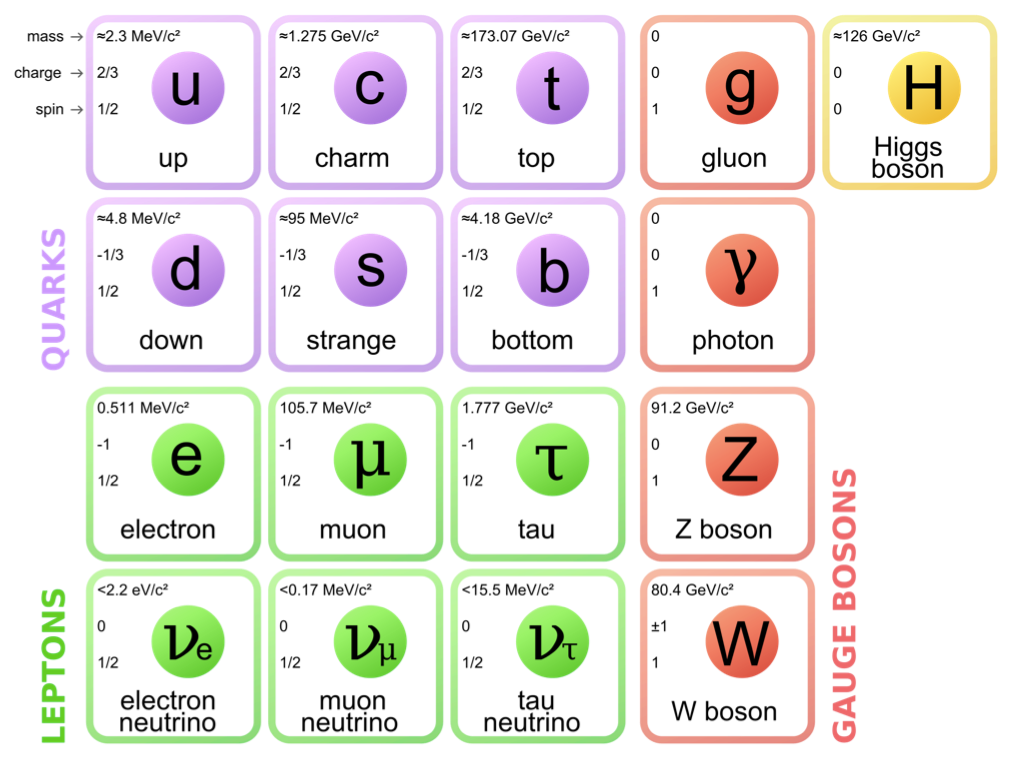
\includegraphics[width=0.8\textwidth]{Introduction/figs/SM.png}
\caption{A scheme of the fundamental particles in the SM with their properties~\cite{SM_particles}.}
\label{fig:SMparticles}
\end{figure}

Due to the asymptotic freedom of the strong interaction quarks cannot be observed in isolation and 
are always combined with other quarks to form color singlets~\cite{Gross:1973id}. Non-fundamental particles
composed of quarks are called hadrons and are classified into two groups: mesons, where the colour singlet
is achieved by the combination of a quark and an antiquark (\quark\quarkbar), and baryons
formed from three quarks (\quark\quark\quark) of different colours.
Recently, in 2014 and 2015 evidence for new states, formed by four and five quarks, was found~\cite{Aaij:2014jqa,Aaij:2015tga}.
%Recently evidence for particles composed by 4 quarks was also found~\cite{}.


\section{The electroweak interaction}
\label{sec:EMandEW}

The electromagnetic interaction is responsible for binding electrons and nuclei
together to form atoms and its mediator is the photon.
%
%,which also sets the range of the EM force to infinity, since this is proportional to the inverse of the mediator mass.
%In fact Heisenberg's Uncertainty Principle tells us that $\Delta E \Delta t > \hbar$, namely virtual particles
%of energy $\Delta E$ are allowed to exist for time intervals inferior to $\Delta t$. Thus, since particles can move
%at most at the speed of light, $c = 299792458$ ms$^{-1}$~\cite{PDG2014}, this also sets a relation between the length 
%of time and space in which a virtual photons can exist ($\Delta t > \hbar / (mc^2)$). As virtual photons can be very
%close to the mass shell, this results in a very long lifetime. The EM force has therefore an infinite range.
%
The weak interaction is responsible for the $\beta$ decay of nuclei and is mediated
by the exchange of $W^\pm$ and $Z^0$ bosons. Unlike the electromagnetic force,
that affects only charged particles, all known fermions interact through the weak interaction.
The weak interaction is also the only one that violates the parity symmetry, which states that interactions are invariant under
an inversion of spatial coordinates. This symmetry breaking arises from the fact that only left-handed fermions interact through
the weak interaction as discovered by Wu in 1957~\cite{Wu:1957my}. Similarly, the weak interaction
is the only one that also breaks the CP symmetry, which combines parity transformations and charge conjugation.
This is particularly interesting because all interactions are believed to be invariant under the CPT transformation, which combines the CP
transformation and time reversal. Hence, breaking CP the weak interaction implies that the process is also not invariant under 
time reversal transformations.

In 1968 Salam, Glashow and Weinberg unified the weak and electromagnetic forces into a single theory, where the coupling
constants of the electromagnetic, $e$, and weak, $g$, interactions are related through the weak mixing angle, $\theta_W$
by the relation $g\sin\theta_W = e$~\cite{PDG2014}. 
%
The electroweak symmetry is spontaneously broken by the Higgs
mechanism~\cite{Strocchi:1977za} and this causes the $W^\pm$ and \Z bosons to become massive (see Tab.~\ref{tab:interactions}) 
and consequently the weak force has a very short range. In fact, using Heisenberg's Principle, $\Delta E \Delta t > \hbar$, 
together with Einstein's formula $\Delta E = m c^2$, which relates mass and energy, and knowing that the maximum 
space that a particle can cover in a time $\Delta t$ is $r \sim c \Delta t$, qualitatively $r \sim \hbar / mc$. In this picture
the carriers of the weak force can travel $r \sim 2 \cdot 10^{-3}$~fm. In contrast, the photon must be massless in the theory, 
which accounts for the long range of the electromagnetic force.
%
The EW interactions are divided into Charged Currents (CC) and Neutral
Currents (NC). In the first group, quarks and leptons interact with the $W^\pm$ bosons, producing decays such as
$\mu^+(\mu^-) \rightarrow e^+ \nu_e \overline{\nu}_\mu (e^- \overline{\nu}_e \nu_\mu)$ and $n (\overline{n}) \rightarrow p e^- \overline{\nu}_e (\overline{p} e^+ \nu_e)$.
The study of these processes confirmed that only the left-handed (right-handed) component of fermions (anti-fermions)
takes part in weak processes. The CC interactions have a peculiarity: they are the only interactions in the SM that violate
flavour conservation at tree level, while any other interaction not conserving flavour has to proceed through
higher order processes. The second group of EW interactions, NC, corresponds to diagrams mediated by a photon or a \Z 
boson interacting with a fermion and its anti-fermion.



\section{Flavour and the CKM matrix}
\label{sec:flavour}

``Flavour" in particle physics refers to the quark/lepton composition of a particle. The introduction of flavour quantum numbers
was motivated in order to explain why some decays, although kinematically allowed, had never been observed. All leptons are
assigned a quantum number $L_\ell = 1$ (where $\ell = e,\mu,\tau$), which in the SM is conserved by all interactions.
This conservation is experimentally well established; for example decays like $\mu^- \rightarrow e^- \gamma $ have never
been observed.
%This is explained by the fact that the lepton number in the initial
%and final state are different and the decay would violate lepton flavour.
%
In the hadronic sector particles carry flavour numbers described as:
%
 \begin{itemize}
 \item \emph{Isospin}: $I_3 = 1/2$ for the up quark and $I_3 = -1/2$ for the down quark;
 \item \emph{Strangeness}: $S = -(n_s - \bar{n}_s)$, where $n_s$ and $\bar{n}_s$ are the numbers of strange
 and anti-strange quarks respectively;
 \item \emph{charmness, bottomness, topness}: in analogy to strangeness
 they are respectively defined as $C = -(n_c - \bar{n}_c)$, $B = -(n_b - \bar{n}_b)$, $T = -(n_t - \bar{n}_t)$.
 \end{itemize}

As mentioned previously, in the SM the only interaction violating flavour conservation is the weak interaction
when mediated by $W^\pm$ bosons.

Measuring branching fractions of weak decays such as $\pi \to \mu \nu_\mu$ and $K \to \mu \nu_\mu$, corresponding
respectively to $ud\to\mu\nu_\mu$ and $us\to\mu\nu_\mu$ processes, suggested the existence of more than one
coupling constant for different quarks. Nicola Cabibbo, in order to preserve the universality
of weak interactions, suggested that the differences could arise from the fact that
the doublets participating in the weak interactions are an admixture of the mass eigenstates~\cite{PDG2014,Cabibbo:1963yz}. 
He therefore introduced the Cabibbo angle, $\theta_c$, proposing that mass eigenstates participating 
in the weak interaction are rotated with respect to the flavour eigenstates.
%
\begin{equation}
\left( \begin{array}{c}
d_W \\ s_W
\end{array} \right) =
\left( \begin{array}{cc}
\cos \theta_c  & \sin \theta_c\\
-\sin \theta_c & \cos \theta_c
\end{array} \right)
\left( \begin{array}{c}
d \\ s
\end{array} \right) = 
\left( \begin{array}{c}
\cos\theta_c \cdot d + \sin \theta_c \cdot s \\
\cos \theta_c \cdot s - \sin \theta_c \cdot d
\end{array} \right)
\end{equation}

In a six quark system one angle is not sufficient to describe a rotation but the mixing can be generalised
using a $3 \times 3$ unitary matrix, called the CKM matrix, from the names of Cabibbo, Kobayashi and Maskawa~\cite{Cabibbo:1963yz,Kobayashi:1973fv}.
The unitarity of the matrix is required to preserve the universality of the weak interaction. Theoretically, a $N \times N$ complex
matrix depends on $2 \cdot N^2$ real parameters. Requiring unitarity ($AA^\dagger = A(A^*)^T = I$), the number
of independent parameters left is 
\begin{equation}
(N - 1)^2 = \underbrace{\frac{1}{2}N(N-1)}_\text{Number of mixing angles} + \underbrace{\frac{1}{2}(N-1)(N-2)}_\text{Number of complex phases}.
\end{equation}  
Therefore a $3 \times 3$ matrix depends then on 4 real parameters: three real constants 
and one imaginary phase. The imaginary phase generates the \mbox{CP-violation} which was
observed in weak interactions.
Figure~\ref{fig:ch_currents_ckm} displays examples of CC processes together with the CKM elements associated with their vertices.
%
\begin{figure}[h!]
\centering 
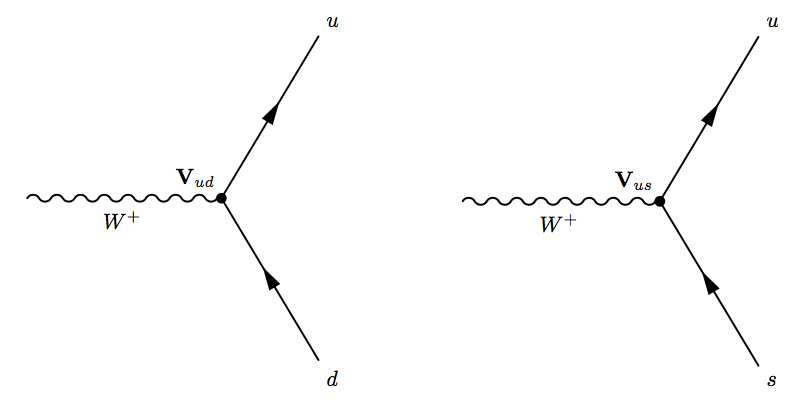
\includegraphics[width=0.6\textwidth]{Introduction/figs/ch_currents_ckm.png}
\caption{Feynman diagrams with CKM weights on weak interaction vertices as defined in Eq.~\ref{eq:CKM}.}
\label{fig:ch_currents_ckm}
\end{figure}
%
Equation~\ref{eq:CKM} reports the most recent measured values of its elements~\cite{PDG2014}
together with the widely used Wolfenstein parameterisation which highlights the hierarchical structure of the matrix.
In fact, elements on the diagonal, corresponding to transitions between quarks of the same generation,
are approximately 1 and become smaller and smaller going farther from the diagonal.
In the formula $\rho$, $A$, and $\lambda$ are the real constants and $\eta$ the imaginary phase 
and Eq.~\ref{params} shows how they are related to the three mixing angles; terms further from the diagonal 
are proportional to higher powers of $\lambda$.
%
\begin{eqnarray}
& V = \left( \begin{array}{ccc}
V_{ud} & V_{us} & V_{ub}  \\
V_{cd} & V_{cs} & V_{cb}  \\
V_{td} & V_{ts} & V_{tb}  
 \end{array} \right) = \left( \begin{array}{ccc}
0.9743 \pm 0.0002 & 0.2253 \pm 0.0007 & 0.0035^{+0.0002}_{-0.001} \\
 0.2252 \pm 0.0007 & 0.9734 \pm 0.0002 & 0.00412^{+0.0011}_{-0.0005} \\
 0.0087 \pm 0.0003 & 0.0404^{+0.0011}_{-0.0005} & 0.99915^{+0.00002}_{-0.00004} 
 \end{array} \right) \nonumber \\ [8pt]
& = \left( \begin{array}{ccc}
1 - \lambda^2/2 & \lambda  & A \lambda^3(\rho -i\eta) \\
-\lambda & 1 - \lambda^2/2 & A\lambda^2 \\
A \lambda^3(1 - \rho -i\eta) & A\lambda^2 & 1 
\end{array} \right) + O(\lambda^4)
\label{eq:CKM}
\end{eqnarray}
%
\begin{equation}
\begin{array}{rl}
\lambda & = \sin(\theta_{12}) = \sin(\theta_c) \\
A\lambda^2 & = \sin(\theta_{23}) \\
A\lambda^3(\rho - i\eta) & = \sin(\theta_{13})e^{i\delta}
\end{array}
\label{params}
\end{equation}
%
%
%Another feature to note is that, due to the unitarity of the matrix, the transformation has no effect on neutral interactions.
%
%In fact defining $q' = Vq$:
%
%\begin{equation}
%\bar{q}'q' = \bar{q}V^{*}Vq = \bar{q}q.
%\end{equation}
%
%As a result flavour-changing neutral currents are forbidden at tree level in the SM.
%

The unitarity of the CKM matrix imposes constraints to its elements of the form:
\begin{equation}
\sum_i |V_{ik}|^2 = 1 \text{ and } \sum_k V_{ik} V^{*}_{jk} = 0.
\end{equation}
These correspond to constraints on three complex numbers, which can be viewed
as the sides of triangles in the $(\rho,\eta)$ plane; these are called ``unitarity triangles".
The most commonly used unitarity triangle arises from $V_{ud}V^*_{ub} + V_{cd}V^*_{cb} + V_{td}V^*_{tb}=0$.
%\begin{equation}
%V_{ud}V^*_{ub} + V_{cd}V^*_{cb} + V_{td}V^*_{tb}=0.
%\end{equation}
Figure~\ref{fig:unitarity_triangle} shows a representation of such triangle together with
a plot summarising the most up-to-date experimental constraints to its parameters~\cite{Charles:2015gya}.
Due to these unitarity constraints flavour-changing neutral currents
are forbidden at tree level in the SM.

The precise measurement of the parameters of the CKM matrix
is a powerful stability test of the SM and sets a solid basis for new physics
searches in the flavour sector. One of the main goals of the LHCb experiment is to measure precisely
 the angle $\gamma$, which is currently the least constrained by measurements.
 %
\begin{figure}[h!]
\centering 
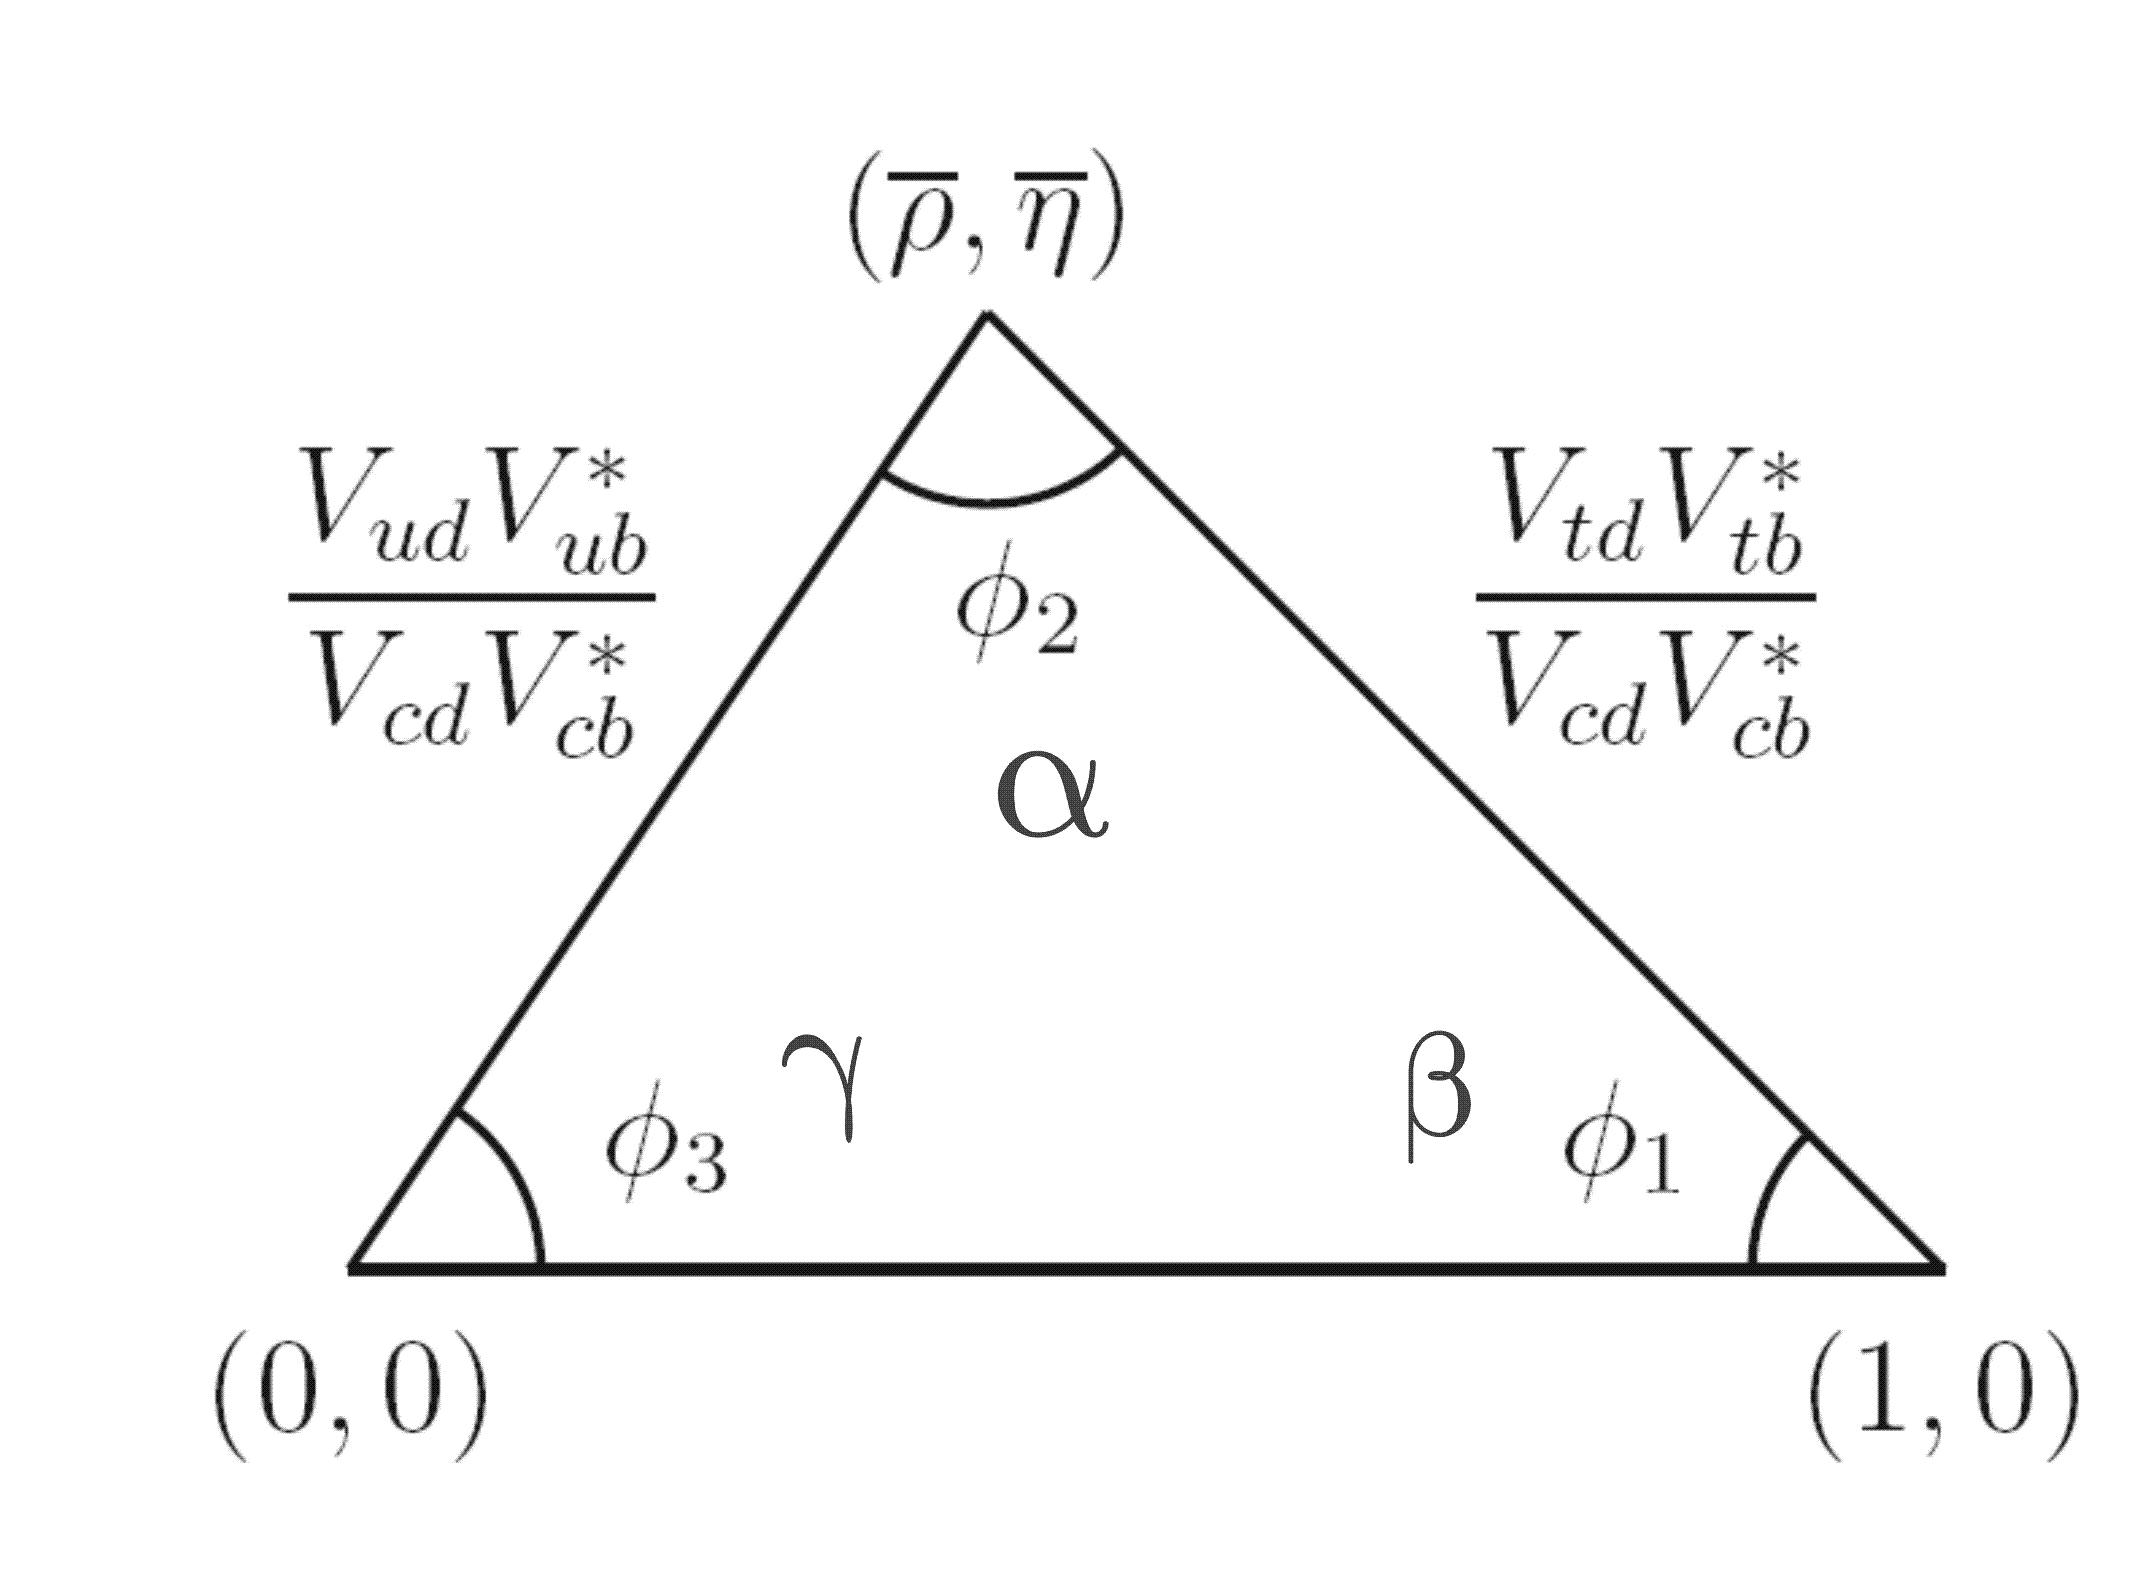
\includegraphics[width=0.5\textwidth]{Introduction/figs/Unitarity_triangle.png}
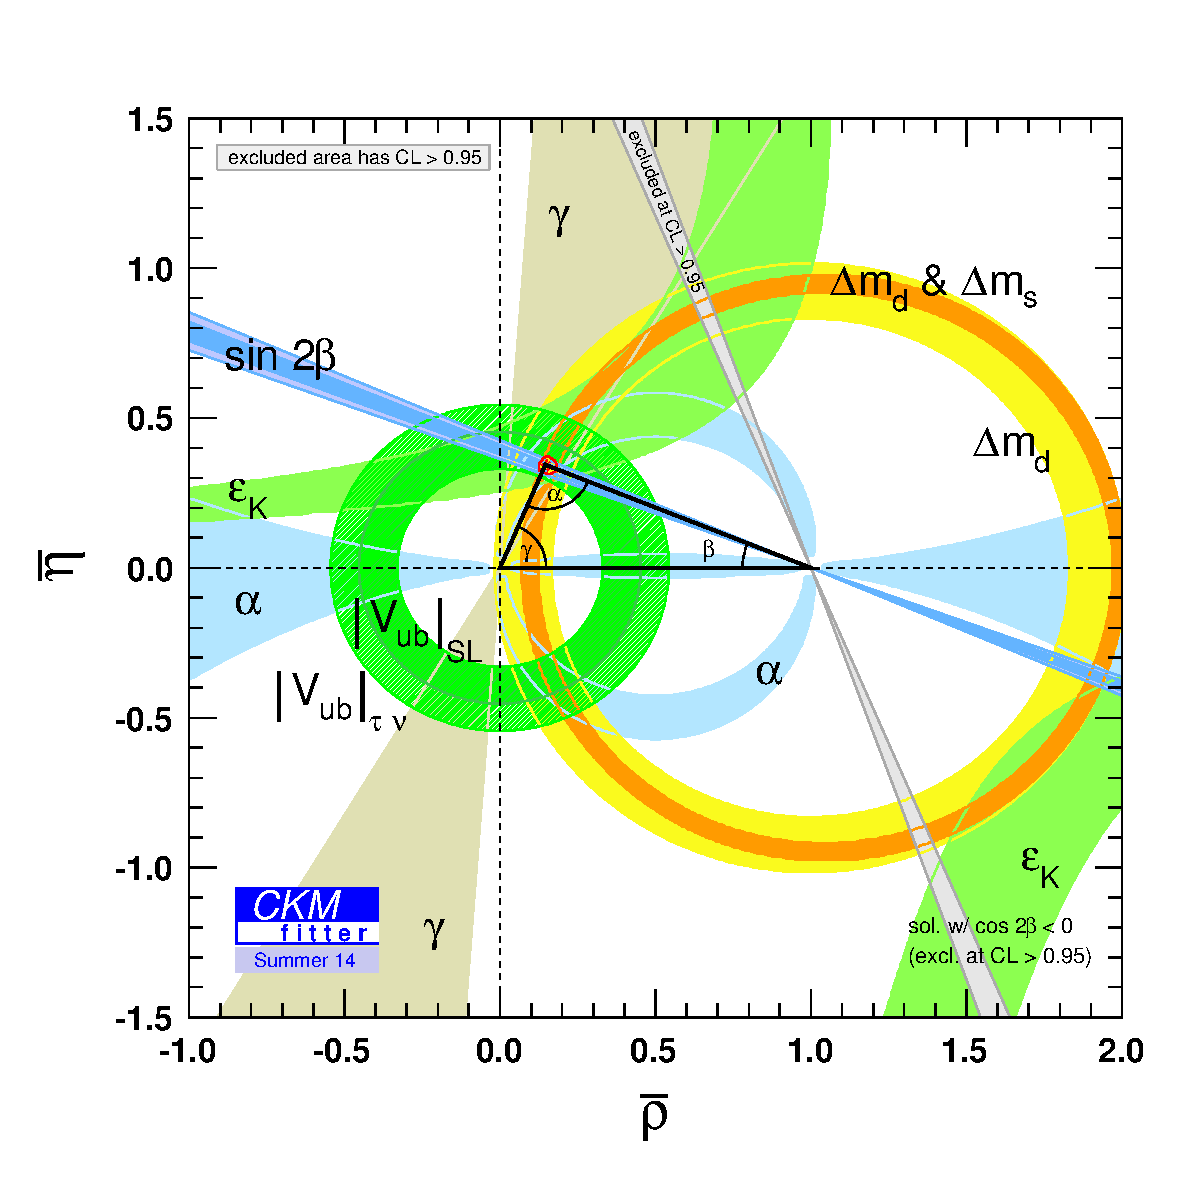
\includegraphics[width=0.7\textwidth]{Introduction/figs/Unitarity_triangle_HFAG.pdf}
\caption{(top) A representation of the unitarity triangle and its parameters.
(bottom) A summary of the most up-to-date measurements of the unitarity triangle parameters~\cite{Charles:2015gya}.}
\label{fig:unitarity_triangle}
\end{figure}
 
 
 
 
\section{The puzzles of the SM}
\label{sec:SMproblems}

Despite the experimental confirmation of many predictions of the SM, the theory has several limitations
and is unable to account for some well-established experimental facts:
%
\begin{itemize}
\item \emph{Dark matter}: experimental evidence tells us that the content of visible matter in the universe is not sufficient
to account for the observed rotation of galaxies~\cite{Zwicky:1933gu}. The most natural way to solve the problem
is the hypothesis of a form of matter that interacts with the gravitational field but not with the other SM interactions. 
%Furthermore, studies of the fluctuations of the cosmic microwave background indicate the existence of
%cold dark matter~\cite{Dunkley:2008ie}.
%formed of particles which do not interact through the SM forces and
%for which there is no SM candidate.
%
\item \emph{Matter-antimatter asymmetry}: a large asymmetry is observed between the quantity of matter 
and antimatter in the universe, $O(10^{-9})$. Assuming that both were equally created in the initial state of 
the universe, a condition such as the violation of the CP symmetry is necessary to account for the observed
imbalance. However, the magnitude of CP violation predicted by the SM, $O(10^{-20})$, is not sufficient to 
account for the observed asymmetry~\cite{Gavela:1993ts}.
%
\item \emph{Gravity}: even though the gravitational force was the first to be discovered 
this is not included in the SM. % as it can be neglected at the EW scale. 
When introducing gravity into the framework of QFT the
theory diverges. On the other hand gravity becomes irrelevant for the small masses 
of particles and can be neglected to a good approximation at the EW energy scale.
Many attempts have been made but there is not yet a consistent theoretical framework through which
 gravity can be introduced in the SM~\cite{Carlip:2001wq}. 
%
\item \emph{Neutrino oscillation}: measurements of solar and atmospheric neutrinos, as well as
neutrinos from nuclear reactors, have established that neutrinos can change flavour while propagating in space.
This is not predicted in the SM, in fact in the SM neutrinos are massless, while an oscillation requires a non-zero
 mass~\cite{Maltoni:2011zz,Cleveland:1998nv,Fukuda:1998mi,Eguchi:2002dm}.
%
\item \emph{The hierarchy problem}: the mass of a scalar (spin 0) particle, such as the Higgs boson,
suffers from quantum corrections due to the physics at high energy scales. As new physics can appear
anywhere up to the Planck scale, $\sim 10^{19}$~\gev, at which gravity cannot be neglected any more,
these corrections can be very large and it would require a high level of fine-tuning for them to cancel 
out and give such a small value as the one measured for the
Higgs Mass, $\sim 126$~\gevcc~\cite{Feng:2013pwa,Aad:2012tfa}. 
%This is considered unnatural by many physicists and pushes them
%to look for further motivations.
%
\end{itemize}
%
In conclusion, even though the SM has been very successful in describing the properties of the observed particles
and their interactions so far, because of its many puzzles, it is believed only to be part of a more general theory 
or only to be valid up to a certain energy scale. %Many theoretical models expect New Physics (NP) to enter at the TeV scale.

\subsection{The flavour problem}

%As mentioned in Sec.~\ref{sec:flavour}, flavour conservation is well experimentally established but it does not
%have a strong theoretical otivation in the Standard Model.
Flavour Changing Charged Currents (FCCC) that are mediated by the $W^\pm$ bosons are the only sources of flavour changing interactions 
in the SM and, in particular, of generation changing interactions, where a quark or a lepton of a family transforms
into one of an other family. Another class of processes is the Flavour Changing Neutral Currents (FCNCs), \emph{e.g.} transitions from a
\bquark quark with a charge of -1/3 to a \squark or \dquark quark with the same charge. Examples of FCNC transitions in the quark
and lepton sector are shown in Fig.~\ref{fig:neutr_curr}.
%
\begin{figure}[h!]
\centering 
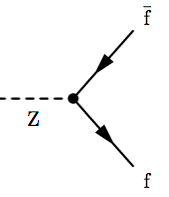
\includegraphics[width=0.25\textwidth]{Introduction/figs/Z2ffbar.png}
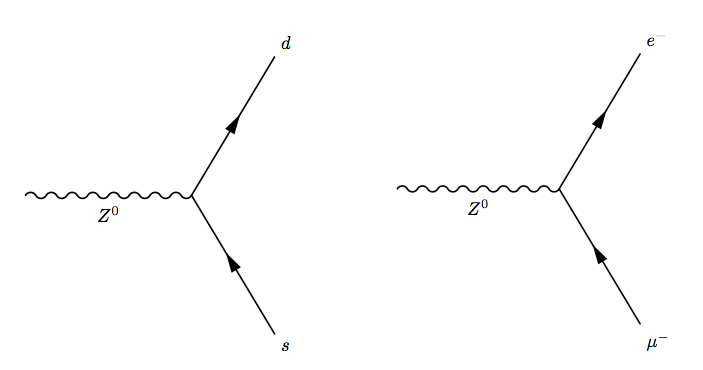
\includegraphics[width=0.6\textwidth]{Introduction/figs/neutral_current_proc.png}
\caption{Feynman diagrams of a neutral current allowed in the SM (left), where$f$ represents any fermion,
and FCNCs processes forbidden in the SM (center-right).}
\label{fig:neutr_curr}
\end{figure}
%
FCNCs are experimentally observed to be highly suppressed which derives from the unitarity of the CKM matrix,
however there is no fundamental reason why there cannot be FCNCs at tree level. In fact the CKM matrix
could be part of a larger matrix involving for example quark-lepton terms. This would introduce
new sources of FCNCs but could also allow for natural explanations of the equality of the proton and electron charges.
Furthermore, the observation of neutrino oscillation proves that flavour is not always conserved
suggesting flavour structures beyond the SM. Finally, the values of the terms of the CKM matrix and the PMNS
matrix~\cite{Pontecorvo:1967fh,Maki:1962mu}, which is the mixing-matrix equivalent to the CKM in the lepton sector,
are not explained in the SM but have to be measured experimentally. These open problems motivate searches for flavour
symmetries and deeper motivations for flavour conservation. 

\section{Beyond the Standard Model}

From the previous sections it is evident that, despite the great success of the SM, there is a need to explore theories Beyond the SM (BSM).
Among the most promising approaches there are those involving Super-Symmetry (SUSY)~\cite{Fayet:1976cr} and extra-dimensions~\cite{Randall:1999ee}. 
%
In SUSY new degrees of freedom are introduced to suppress the diverging terms of the Higgs mass. This theory
assumes that for each fermion there is a corresponding boson and, since bosons and fermions contribute with opposite
sign to the mass term, these would naturally cancel out. Super-Symmetry also provides a candidate for dark
matter. In fact the lightest Super-Symmetric particle, the neutralino, which in R-parity~\cite{Ellis:1984gi} conserving 
variants of the theory must be stable, is a weakly interacting and potentially massive particle.
%
The idea to introduce extra-dimensions was triggered by the fact that gravity is not relevant in particle physics but it would 
be natural if all forces had similar strength. By adding extra dimensions to the normal three spatial dimensions, one can restore 
the strength of gravity, as this could be dispersed by the wider space available.
%
In all these approaches, constraints to masses and couplings must be imposed to maintain
compatibility with the SM at the electroweak scale and the existing experimental observations.

\subsection{Flavour and BSM theories}

Most BSM theories predict processes violating flavour conservation. Therefore, the observation or
non-observation of these processes can give important information about new physics.
BSM theories can be classified according to the amount of flavour violation they introduce.
The first class of models to consider is that with Minimal Flavour Violation (MFV).
These are models in which the only sources of flavour changing transitions are governed by the
CKM matrix and the CKM phase is the only source of CP violation.
This definition is driven by the fact that usually a solution of the hierarchy problem is expected
at the TeV scale, while the very small amount of flavour violation observed in measurements
seems to indicate that the SM would remain valid up to much higher energy scales.
It is therefore assumed that new physics must respect flavour symmetry principles, which also makes these
types of models naturally compatible with the SM. Examples of such models include the MSSM
with minimal flavour violation and the SM with one extra-dimension. Reviews of MFV models
are presented in Refs.~\cite{Isidori:2012ts,Buras:2003jf}.
%
%The MFV hypothesis provides a way to resolve the tension between expectation, driven by naturalness arguments,
%that NP should be at the \tev~scale and limits on FCNC processes that point to much higher scales.
%
A powerful test of MFV is provided by the study of ratios between $\bquark\to\dquark$ and $\bquark\to\squark$
transitions, because their Hamiltonians share the same structure. One particularly important example is the ratio between the 
decay rates of $\Bz$ and $\Bs$ into dimuons~\cite{TomRDreview}, as this is a purely leptonic decay free from hadronic uncertainties.
In the SM such ratios are approximately equal to $|V_{td}/V_{td}| \sim 1/25$, only modified by phase space and hadronic
matrix elements, while they can take very different values in non-MFV models.

In the quest for new physics an important role is also played by simplified models
as an intermediate model building step. Instead of constructing theories valid up to the GUT scale
one can consider simplified models, where the SM is extended by the addition of new degrees of freedom
with a limited number of parameters. Such models are easier to constrain but can nevertheless point
in the right direction to build more complete theories. The choice of the new sector to add can be driven 
by the need to explain existing tensions between measurements and SM predictions or by theoretical prejudice.
%
Two models especially relevant when studying rare decays, which are the main topic of this thesis, are 
$Z'$-penguins and leptoquarks. A $Z'$-penguin is a FCNC process involving a neutral field arising from an extra 
U(1) gauge symmetry, for example U(1)$_{B-L}$, where $B$ and $L$ are the baryon and lepton numbers. 
As for the SM penguins, the $Z'$ field contributes in loops causing modifications of the 
effective couplings with respect to the SM. A survey of $Z'$ models can be found in Ref.~\cite{Buras:2014zga}.
%
Leptoquarks are bosonic particles that carry both quark and lepton flavour quantum numbers, which
for simplicity are assumed to be scalar.
A tree level exchange of a leptoquark induces processes such as $\bquark \to (\squark,\dquark)\ell^+\ell^-$,
and therefore can result in an enhancement of their decay rates with respect to the SM~\cite{Hiller:2014yaa}.
Leptoquarks would also provide a natural explanation for non-universal couplings to leptons.


\section{Rare decays: a tool to search for new physics}
\label{sec:RD_theory}

In the Standard Model FCNC processes are forbidden at tree level but
can occur through loop diagrams such as penguin or \W box diagrams (see Fig.~\ref{fig:penguins}).
The branching fractions of decays going through these processes are small, typically \mbox{$\sim10^{-6}$} 
or lower, and therefore they are called ``rare decays". Additional contributions to the virtual loops
are not necessarily suppressed with respect to the SM component which makes these decays
very sensitive to new physics. This approach to new physics searches is interesting as
new particles could be at high mass scales that are not accessible via direct production at colliders
but their effect could be observed in loops.
Radiative and penguin decays are particularly interesting because they are theoretically
well understood, which allows precise comparisons with measurements. Furthermore, they provide
a large quantity of observables that can be affected by new physics, not only decay rates, but also 
CP asymmetries and angular observables such as forward-backward asymmetries. The joint
analysis of different observables can help to build a consistent picture and rule out specific models.
%
\begin{figure}[h!]
\centering
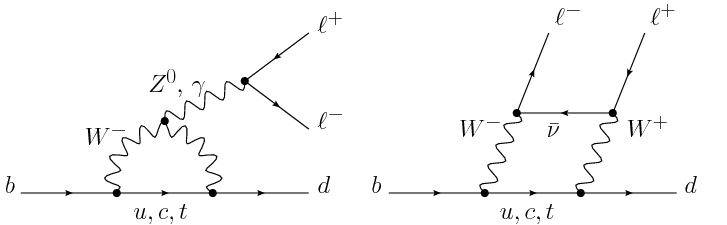
\includegraphics[width=0.9\textwidth]{Introduction/figs/penguin_general.png}
\caption{Loop Feynmann diagrams allowing $\bquark \to \dquark$ FCNC 
processes: penguin diagram (left) and \W box (right).}
\label{fig:penguins}
\end{figure}

\subsection{Theoretical framework: the effective Hamiltonian}
\label{sec:Effective_Hamiltonian}

Rare decays of \bquark hadrons are governed by an interplay between weak
and strong interactions.
%The QCD corrections that arise from hard gluon exchange bring large logarithms
%of the form $\alpha_s^n(m_b)\log^m(m_b/M)$, where $M = m_t$ or $M = m_W$.
%A suitable framework to achieve the necessary resummation of these logarithms
%in an effective low-energy theory with five quarks.
%The QCD corrections that arise from hard gluon exchange bring large contributions
%large logarithms of the form $\alpha_s^n(m_b)\log^m(m_b/M)$, where $M = m_t$ or $M = m_W$.
The large masses of the $W^\pm$ and $Z^0$ bosons and top quark compared to that of the \bquark quark allow
the construction of an effective theory that divides the problem of calculating
weak decay amplitudes into two parts: ``short-distance" and ``long-distance" effects separated
at an energy scale $\mu$. The first part, dealing with short distance physics, handles
perturbative contributions due to energy scales above the \bquark mass. The second part
typically deals with non-perturbative contributions. 
A classic example of an effective theory is the Fermi theory of weak interactions
which describes the $\beta$ decay in terms of a four-fermion interaction,
where the short distance physics is hidden into a point-like vertex as illustrated in Fig.~\ref{fig:fermi_theory}.
\begin{figure}[h!]
\centering
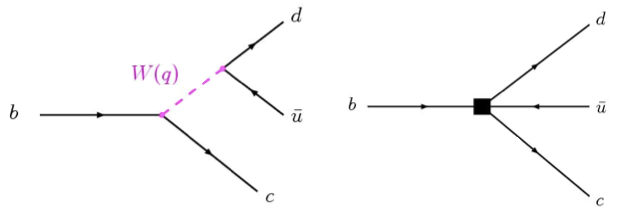
\includegraphics[width=0.7\textwidth]{Introduction/figs/fermi_theory.png}
\caption{Example of a Fermi theory in which the full theory (left) is divided into (right) a
short distance contribution, hidden in the vertex, and a long distance contribution.}
\label{fig:fermi_theory}
\end{figure}
\clearpage
The effective Hamiltonian~\cite{Chetyrkin:1996vx} relevant to
$\bquark\to\squark/\dquark \gamma$ and  $\bquark\to\squark/\dquark \ell^+\ell^-$
transitions can be written as:
%
\begin{equation}
\mathcal{H}_{eff} = \frac{-4G_F}{\sqrt{2}} \left[ \lambda^t_q \sum C_i(\mu,M)\mathcal{O}_i(\mu)
+ \lambda^u_q \sum C_i(\mu,M)(\mathcal{O}_i(\mu) - \mathcal{O}_i^u(\mu)) \right],
\end{equation}
%
where $G_F$ denotes the Fermi coupling constant and the $\lambda$ constants are the CKM factors,  
$\lambda^t_q = V_{tb}V_{tq}^*$ and  $\lambda^u_q = V_{ub}V_{uq}^*$. In $\bquark\to\squark$ quark transitions, 
which are the main topic of this thesis, the doubly Cabibbo-suppressed contributions can be neglected as 
$\lambda^u_s << \lambda^t_s$. To obtain this formula the Operator Product Expansion (OPE)~\cite{Buchalla:1995vs} method
is used, which implements a summation over all contributing operators weighted by corresponding constants
called Wilson coefficients. In this Hamiltonian the long-distance contributions are described by the 
operators, $\mathcal{O}_i$, while the short-distance physics is encoded in the Wilson 
coefficients, $C_i$. Operators and coefficients are evaluated at the renormalisation scale $\mu$.
Any particle that contributes to the decay and has a mass greater than the scale $\mu$ will affect the value 
of at least one of the Wilson coefficients, including SM particles as the top quark.

In order to describe SM processes the effective theory must be matched with the SM by requiring 
the equality between each term in effective theory and the full theoretical calculation at a matching 
scale, typically the EW scale ($\mu_W$). Then, using the scale independence of the
effective Hamiltonian, one can derive a renormalisation group equation for the Wilson coefficients~\cite{Buras:1998raa}.
%
%
%\begin{equation}
%\mu \frac{\deriv}{\deriv \mu} C_i(\mu) = \gamma_{ij}C_j(\mu),
%\end{equation}
%
%where the matrix $\gamma$ is the anomalous dimensions matrix of the operators $\mathcal{O}_i$.
%At leading order the solution is given by~\cite{Buras:1998raa}:
%
%\begin{equation}
%C_i(\mu) = \left[ \frac{\alpha_s(\mu_W)}{\alpha_s(\mu)}\right]^{\frac{\gamma^0_{ii}}{2\beta_0}} C_i(\mu_W) = \left[ \frac{1}{1 + \beta_0\frac{\alpha_s(\mu)}{4\pi}ln\frac{\mu_W^2}{\mu^2}} \right]^{\frac{\gamma^0_{ii}}{2\beta_0}} C_i(\mu_W),
%\end{equation}
%
%where $\alpha_s$ is the strong coupling constant.
%
Taking into account only SM contributions and using $\mu_W = m_b$, the Wilson coefficients have values:
%
\begin{equation}
\begin{array}{ccc}
C_7^{SM} = -0.3, & C_9^{SM} = 4.2, & C_{10}^{SM} = -4.2
\end{array}
\end{equation}
%
and new physics contributions appear in the Wilson coefficients in the form of additive factors:
\begin{equation}
 C_i = C_i^{NP} + C_i^{SM}.
\end{equation}

The amplitudes of exclusive hadronic decays can be calculated as the expectation 
values of the effective Hamiltonian. Given an initial state $I$ and a final state $F$
\mbox{(\emph{e.g.}: $I = \Bz$ and $F=\Kstarz\mumu$)} the decay amplitude can be calculated as
%
\begin{equation}
\begin{array}{rl}
A(I\to F) &= \langle I | \mathcal{H}_{eff} | F \rangle = \\
&= \frac{G_F}{\sqrt{2}} \sum V_{CKM}^i \underbrace{C_i(\mu)}_{\shortstack{Perturbative \\ Includes new physics}} \cdot  \underbrace{\langle I | \mathcal{O}_i(\mu) | F \rangle}_{\shortstack{Non-preturbative \\ Known physics}},
\end{array}
\end{equation}
where $\langle I | \mathcal{O}_i(\mu) | F \rangle$ are the hadronic matrix elements also called  ``form factors".
These can be evaluated using non perturbative methods such as lattice calculations.
However, due to the limitations of these methods, they represent the dominant source 
of uncertainty in theoretical calculations.

\subsection{Operators}
\label{sec:operators}

Separating the left- and right-handed components the effective Hamiltonian is
%for $\bquark\to\squark\ell^+\ell^-$ transitions is
%
\begin{equation}
\mathcal{H}_{eff} = \frac{4G_F}{\sqrt{2}} V_{tb}V^*_{ts} \frac{\alpha_e}{4\pi} \sum_{i=1}^{10} \left[ C_i \mathcal{O}_i  +  C'_i \mathcal{O}'_i \right].
\end{equation}
%
%where the $V_{ub}$ and $V_{bs}$ are the factors of the CKM matrix.
A complete basis is given by a set of 10 operators, where $\mathcal{O}_{1,2}$ are the tree level W operators;
$\mathcal{O}_{3-6,8}$ are penguin diagrams mediated by gluons; and $\mathcal{O}_{7,9,10}$, which are the operators
that are relevant for radiative and leptonic penguin processes are defined as~\cite{TomRDreview}:
%S is Higgs scalar penguins and P pseudo-scalar penguin
%
\begin{equation}
\begin{array}{ll}
 \mathcal{O}_7 = \frac{m_b}{e} (\bar{s} \sigma^{\mu\nu}P_Rb)F_{\mu\nu},  		& \mathcal{O}_7' = \frac{m_b}{e} (\bar{s} \sigma^{\mu\nu}P_Lb)F_{\mu\nu}, \\
%\mathcal{O}_8 = g_s\frac{m_b}{e} (\bar{s} \sigma^{\mu\nu}P_RT^ab)G^a_{\mu\nu}  	& \mathcal{O}_8' = g_s\frac{m_b}{e} (\bar{s} \sigma^{\mu\nu}P_LT^ab)G^a_{\mu\nu} \\
\mathcal{O}_9 = (\bar{s} \gamma_{\mu}P_Lb)(\bar{\ell}\gamma^\mu\ell), 			& \mathcal{O}_9' = (\bar{s} \gamma_{\mu}P_Rb)(\bar{\ell}\gamma^\mu\ell), \\
\mathcal{O}_{10} = (\bar{s} \gamma_{\mu}P_Lb)(\bar{\ell}\gamma^\mu\gamma_5\ell), 	& \mathcal{O}_{10}' = (\bar{s} \gamma_{\mu}P_Rb)(\bar{\ell}\gamma^\mu\gamma_5\ell),
\end{array}
\end{equation}
%
where $P_{L/R} = (1 \mp \gamma_5)/2$ denote the left- and right-handed chiral projections 
%$T^a$ are the QCD generators 
and $F_{\mu\nu}$ is the electromagnetic field tensor.
%
The $\mathcal{O}'$ operators correspond to right-handed coupling obtained by swapping
$P_R$ and $P_L$ in the equations. In the SM, as well as in MFV models where the
flavour violation is entirely ruled by the CKM matrix, the $C'$ Wilson coefficients 
are suppressed by the strange coupling, $C'_i \sim (m_s / m_b) C_i$.
%
The operator $\mathcal{O}_7$ relates to penguin diagrams that are mediated via a photon.
%and the $\mathcal{O}_8$ by a gluon. The $\mathcal{O}_7$ operator is 
It represents the dominant contribution to the radiative 
$\bquark\to\squark\gamma$ transition and contributes to $\bquark\to\squark\ell^+\ell^-$ processes when
the virtual photon decays into a dilepton pair. The semileptonic $\mathcal{O}_9$ and $ \mathcal{O}_{10}$ 
correspond to penguin diagrams mediated by a $Z^0$ boson and $W$ mediated box diagrams. 
These are the dominant contributions in semileptonic $\bquark\to\squark\ell^+\ell^-$ decays.
The vertices corresponding to the radiative and semileptonic operators are illustrated in Fig.~\ref{fig:vtx_operators}
%
\begin{figure}[h!]
\centering
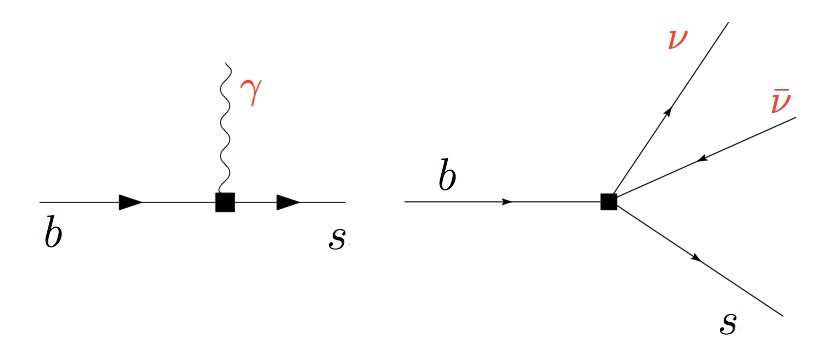
\includegraphics[width=0.6\textwidth]{Introduction/figs/vtx_operators.png}
\caption{Interaction vertices corresponding to the radiative (left) and semileptonic (right) operators.}
\label{fig:vtx_operators}
\end{figure}

It is also common to express the semileptonic operators in a basis with left and right projected leptons
%
\begin{equation}
\begin{array}{ll}
\mathcal{O}_{LL} = ( \mathcal{O}_{9} - \mathcal{O}_{10})/2 & \mathcal{O}_{LR} = ( \mathcal{O}_{9} + \mathcal{O}_{10})/2 \\
\mathcal{O}_{RR} = ( \mathcal{O}'_{9} - \mathcal{O}'_{10})/2 & \mathcal{O}'_{RL} = ( \mathcal{O}'_{9} + \mathcal{O}'_{10})/2 \\
\end{array}
\end{equation}
%
where the Wilson coefficients are redefined as
\begin{equation}
\begin{array}{ll}
C_{LL} = C_{9} - C_{10}, & C_{LR} =  C_{9} + C_{10}, \\
C_{RR} = C'_{9} - C'_{10}, &C'_{RL} =  C'_{9} +C_{10}. \\
\end{array}
\end{equation}
%
This basis is particularly useful in frameworks where BSM physics at a high mass scale
respects the SU(2)$_W$ part of the SM gauge symmetry group.
%For instance, instead of fitting the two parameters $C_9$
%and $C_{10}$, the LL-hypothesis gives the constraint $C_9 + C_{10} = 0$.
%since C9 +C10 = 0 in the standard model there is no sensitivity to CLR and 
%CRR from interference with the standard model in semileptonic decays.
%
Finally, in the picture presented in this section all operators were considered as universal
with respect to the flavour of the involved leptons. However, BSM models often contain sources of
lepton universality violation leading to a split of the same operators depending on the lepton considered:
$C_i \to C_i^e$, $C_i^\mu$, $C_i^\tau$ and $\mathcal{O}_i \to \mathcal{O}_i^e$, $\mathcal{O}_i^\mu$, $\mathcal{O}_i^\tau$. 

\subsection{Phenomenology of $\bquark\to\squark\ell^+\ell^-$ decays}
\label{sec:theo_qsq}

Semileptonic \bquark hadron decays are characterised by two kinematic regimes which
are treated theoretically in different ways; Table~\ref{tab:q2scheme} shows a scheme of the \qsq spectrum.
%
The ``high $q^2$" is the region of low hadron recoil, $\qsq > 15$~\gevgevcccc, and is characterised by 
the energy of the hadron being less than the energy scale of QCD interactions within the meson, 
\mbox{$\Lambda_{QCD} \sim 1$~\gev}. In this region theoretical calculations of $B$ meson decays can be simplified 
by working in the heavy quark limit, $m_b\to\infty$. In this limit a Heavy Quark Effective 
Theory (HQET) can be constructed~\cite{DellaMorte:2015yda} in which the heavy quark interacts 
only via `soft' hadronic processes and an OPE in $1/m_b$ is valid.
%?QCD/mb then shows that the perturbatively calculable parton-level process is the leading 
%contribution to the B0 ?K?0?+?? decay, and the hadronic effects are relatively small. 
%. A heavy-quark expansion in terms of The QCD Factori- sation (QCDF) technique separates the parton-level and %hadronic contributions at the energy scale ??mb, accounting for the ?soft? non-perturbative processes using hadronic %form factors [25].
%
%
%\begin{table}[b]
%\caption{A scheme of the \qsq spectrum.}
%\begin{tabular}{llcrr}
%{\footnotesize $\qsq = 0$ }   &  {\footnotesize  $E_{\Kstarz}  >> \Lambda_{QCD}$	}&  {\footnotesize $\qsq \sim m_{\jpsi,\psitwos}^2$ } & {\footnotesize $E_{\Kstarz}  \sim \Lambda_{QCD}$ } & {\footnotesize $\qsq = (m_B - m_\Kstarz)^2$ } \\
%\hline
%{\footnotesize max. recoil } & {\footnotesize large recoil (SCET) } & {\footnotesize $\cquark\cquarkbar$ resonances } & {\footnotesize low recoil (HQET) } & {\footnotesize zero recoil} \\
%\end{tabular}
%\label{tab:q2scheme}
%\end{table}
\begin{table}[b]
\caption{A scheme of the \qsq spectrum.}
\centering
\begin{tabular}{c|c|c|c}
 \qsq							& $E_{\Kstarz}$	   	&  	Regime 			& 	Valid theory \\ \hline
 $\sim 0$ \gevgevcccc			& $\sim m_B$			&   Max. recoil			&	\multirow{ 2}{*}{SCET}\\ 
 $< 6$	\gevgevcccc			& $>> \Lambda_{QCD}$	&	Large recoil		&		   		\\ \hline
 $\qsq \sim m_{\jpsi,\psitwos}^2$ 	& $\sim 3$ \gev			& 	$\cquark\cquarkbar$ resonances	&  -- 		\\ \hline
 $\qsq > 15$ \gevgevcccc 			& $E_{\Kstarz}  \sim \Lambda_{QCD}$ 			&	Low recoil	&	\multirow{ 2}{*}{HQET}\\
 $\qsq = (m_B - m_\Kstarz)^2$ 		& $E_{\Kstarz} \sim 0$  	&	Zero recoil		&			\\
\end{tabular}
\label{tab:q2scheme}
\end{table}
%
The \mbox{``low $q^2$"} region is where the light spectator quark is energetic and cannot be neglected.
Furthermore, the light quark interacts not only via `soft' hadronic processes, as in HQET, but also via the 
so-called `collinear' hadronic processes.
The boundary of this region can be set at $\sim 7$~\gevgevcccc~ which corresponds to the threshold for 
$\cquark\cquarkbar$ production, $(2m_c)^2$. 
In this region the hadronic interactions are handled by expanding in terms 
of the energy of the emitted energetic hadron, $1/E_h$, forming the so-called Soft-Collinear 
Effective Theory (SCET)~\cite{Bauer:2000yr}.
%
\begin{figure}[h!]
\centering
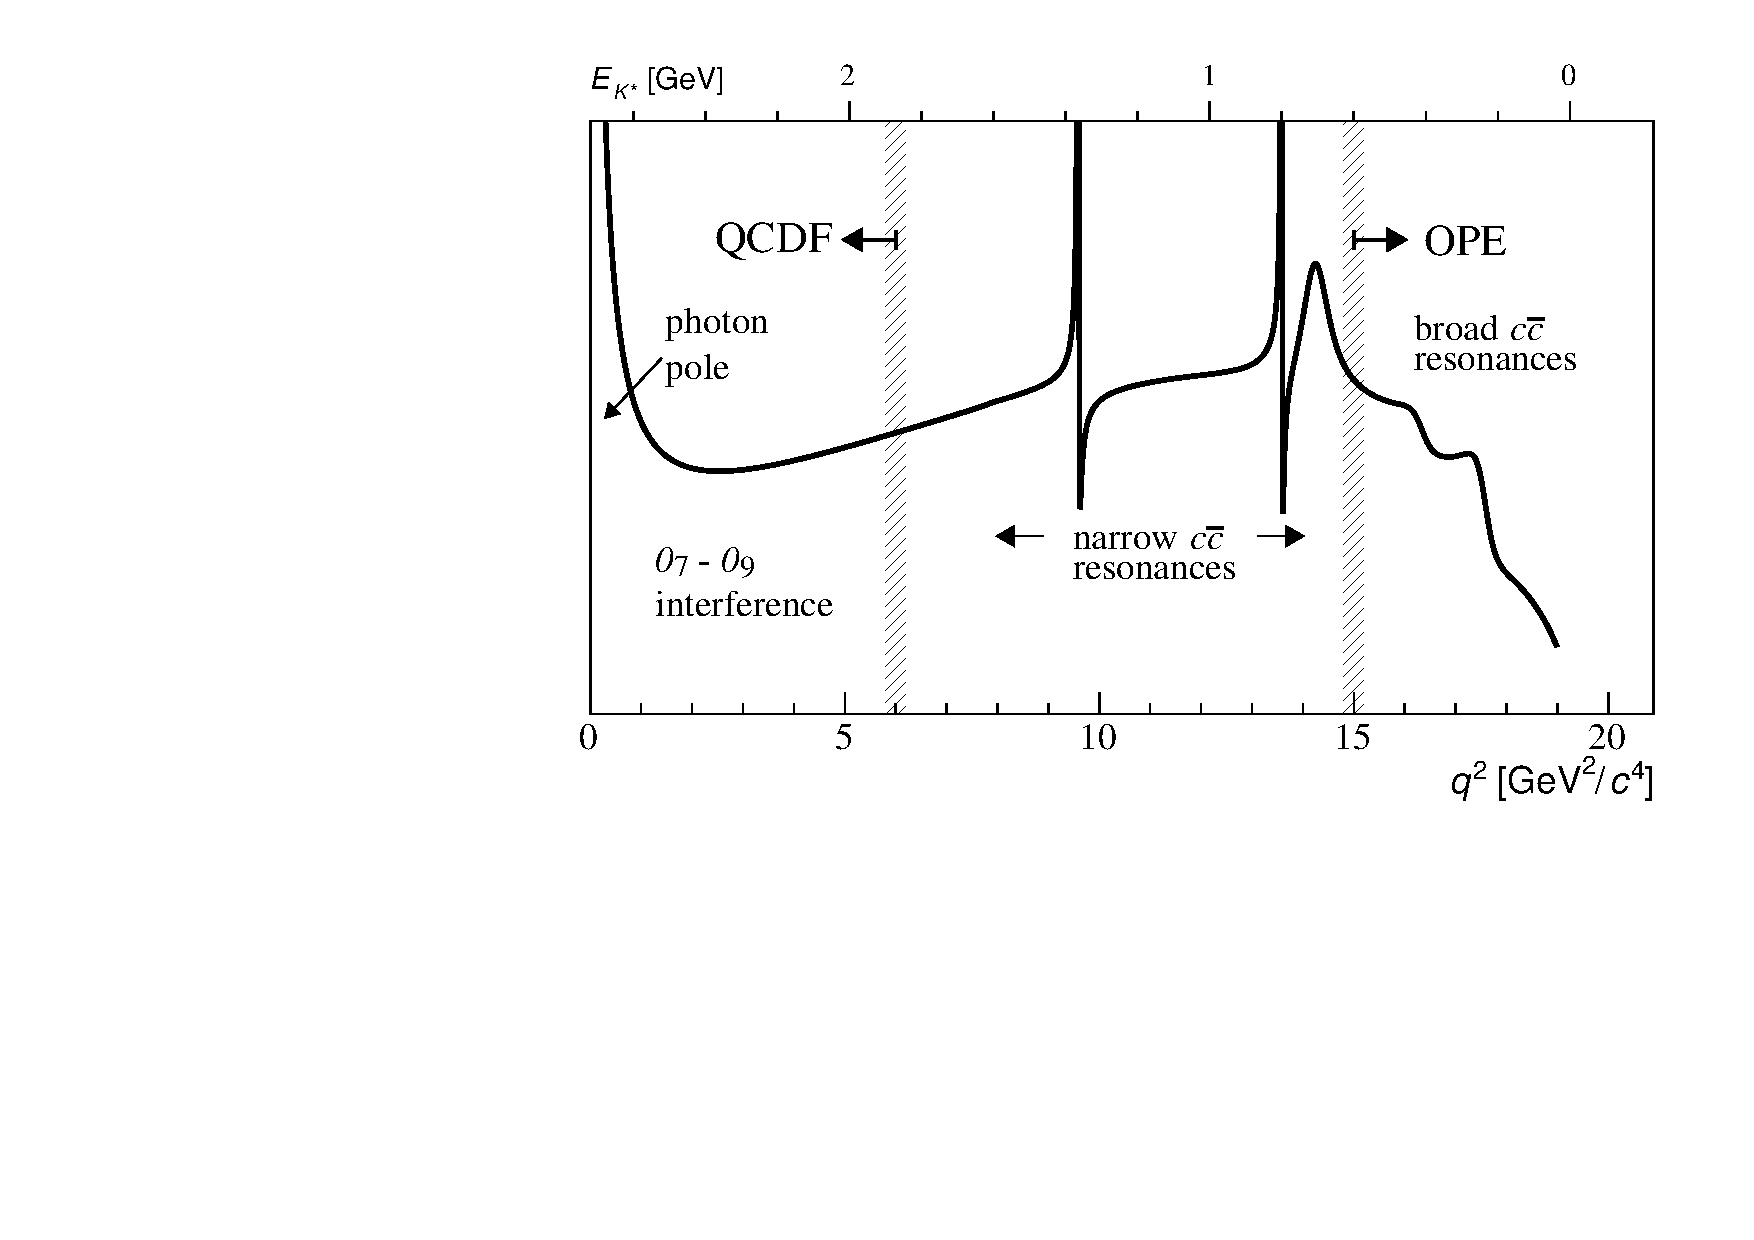
\includegraphics[width=0.8\textwidth]{Introduction/figs/q2spectrum.pdf}
\caption{A typical \qsq spectrum of $\bquark\to\squark\ll$ processes characterised by the photon pole
at  low \qsq, charmonium resonances at central \qsq and broad resonances at high \qsq~\cite{TomRDreview}.}
\label{fig:q2spectrum}
\end{figure}
%
In both regions decay rates can be predicted using the different methods and
the biggest uncertainties come from the limited knowledge of hadronic transition matrix elements.
The intermediate region is characterised by the presence of charmonium resonances, produced though tree 
level $b\to\cbar c s$ transitions and no precise theoretical calculation is available~\cite{Khodjamirian:2010vf}.

As can be seen in Fig.~\ref{fig:q2spectrum} the very low \qsq region is characterised by a peak due
to the virtual photon contribution, associated with $C_7$. In the region $1-6$~\gevgevcccc the 
interference between $C_7$ and $C_9$ becomes large, yielding sensitivity to new physics in $C_9$.
The $7-15$~\gevgevcccc interval is dominated by the charmonium resonances, \jpsi and \psitwos. 
Although these decays can be experimentally vetoed, in
principle charmonia affect the entire \qsq space. Finally, at high \qsq broad charmonium resonances 
can contribute, like those observed by LHCb in $\decay{B^+}{K^+\mumu}$ decays~\cite{LHCB-PAPER-2013-039}.

\subsection{Observables in $\bquark\to\squark\ell^+\ell^-$ decays}
\label{sec:observables}

Rare decays and especially semileptonic $\bquark\to\squark\ell^+\ell^-$ processes offer a number
of observables which can be used to study BSM models.
The most direct effects appear in decay rates that can be enhanced by new physics but the precision on
these measurements is often limited by uncertainties on the non-perturbative part of the calculations.
Therefore, it is important to also look for different observables.
One important class of observables are angular quantities that can often carry complementary 
information with respect to branching ratio measurements. The most basic of these
observable are forward-backward asymmetries that characterise the angular distribution of final particles. 
For the $\Bz\to\Kstarz\mumu$ decay combinations of observables have been proposed
that are independent of form factor uncertainties at leading order order~\cite{TomRDreview}.

Another way to build safe observables is to construct ratios between similar
decays, in which uncertainties due to the hadronisation process cancel out.
These observables include the $R_H$ ratios, between \Bz decays into electrons and muons,
that are described in detail in Ch.~\ref{sec:RKst_theory}.
It is also interesting to compare decays which proceed via the same fundamental process but
where the spectator quark has a different flavour. This is the case of $\Bu\to K^+\mumu$ and $\Bz\to\KS\mumu$
decays, which are both $\bquark\to\squark$ transitions where the spectator quark is a \uquark quark
in the first case and a \dquark quark in the second. The normalised difference of the branching fractions
of these decays is called isospin asymmetry.


\section{Experimental status}
\label{sec:exp_status}

To set the background for the analyses described in this thesis, this section gives a 
brief review of recent results of new physics searches involving rare decays or lepton flavour violation.
Among these, results recently obtained by the \lhcb experiment show a series of anomalies
with respect to the SM that have the potential to yield to BSM scenarios.


\subsection{Dimuon decays of \bquark hadrons}

Decays of $B$ mesons into a pair of muons are two-body decays where the two muons are back to
back in the hadron rest frame. The simple signatures of these decays makes them easy to study
and the fact that they are unaffected by hadronic physics in the final state makes predictions very
clean and precise. Therefore these are essential tests of the SM.
The $\decay{\Bz}{\mumu}$ and $\decay{\Bs}{\mumu}$ decays are FCNCs that can only happen 
via loops and furthermore they are CKM-suppressed, which makes them particularly rare.
In addition, the decay of a pseudo-scalar $B$ meson into two muons has a significant helicity
suppression. The latest SM predictions for these decay rates are~\cite{Bobeth:2013uxa}:
%
\begin{align}
\mathcal{B}(\decay{\Bs}{\mumu}) &= (3.65 \pm 0.23) \times 10^{-9} \text{ and } \\
\mathcal{B}(\decay{\Bz}{\mumu}) &= (1.06 \pm 0.09) \times 10^{-10}.
\end{align}
%
The uncertainties on these values are dominated by the knowledge of the decay constants and 
CKM-elements. BSM models can produce significant enhancement to these decay rates
and the measurement of their ratio is a stringent test of the MFV hypothesis.
A combination of the \lhcb and \cms results gives the values~\cite{CMS:2014xfa}:
%
\begin{align}
\mathcal{B}(\decay{\Bs}{\mumu}) &= (2.8^{+0.7}_{-0.6}) \times 10^{-9} \text{ and } \\
\mathcal{B}(\decay{\Bz}{\mumu}) &= (3.9^{+1.6}_{-1.4}) \times 10^{-10}.
\end{align}
%
%
Neither decay had been previously observed, while now the $\Bs$ decay is observed
with a significance of $6\sigma$ and evidence for the $\Bz$ decay is found
at $3\sigma$ significance level. The measured branching fractions are compatible 
with SM predictions within $2\sigma$ and put strong constraints on the available 
parameter-space for BSM theories. Figure~\ref{fig:bsmumu} shows the fit the dimuon 
invariant mass of $B$ meson candidates where the peaks of the two decays are visible.
%
\begin{figure}[b!]
\centering
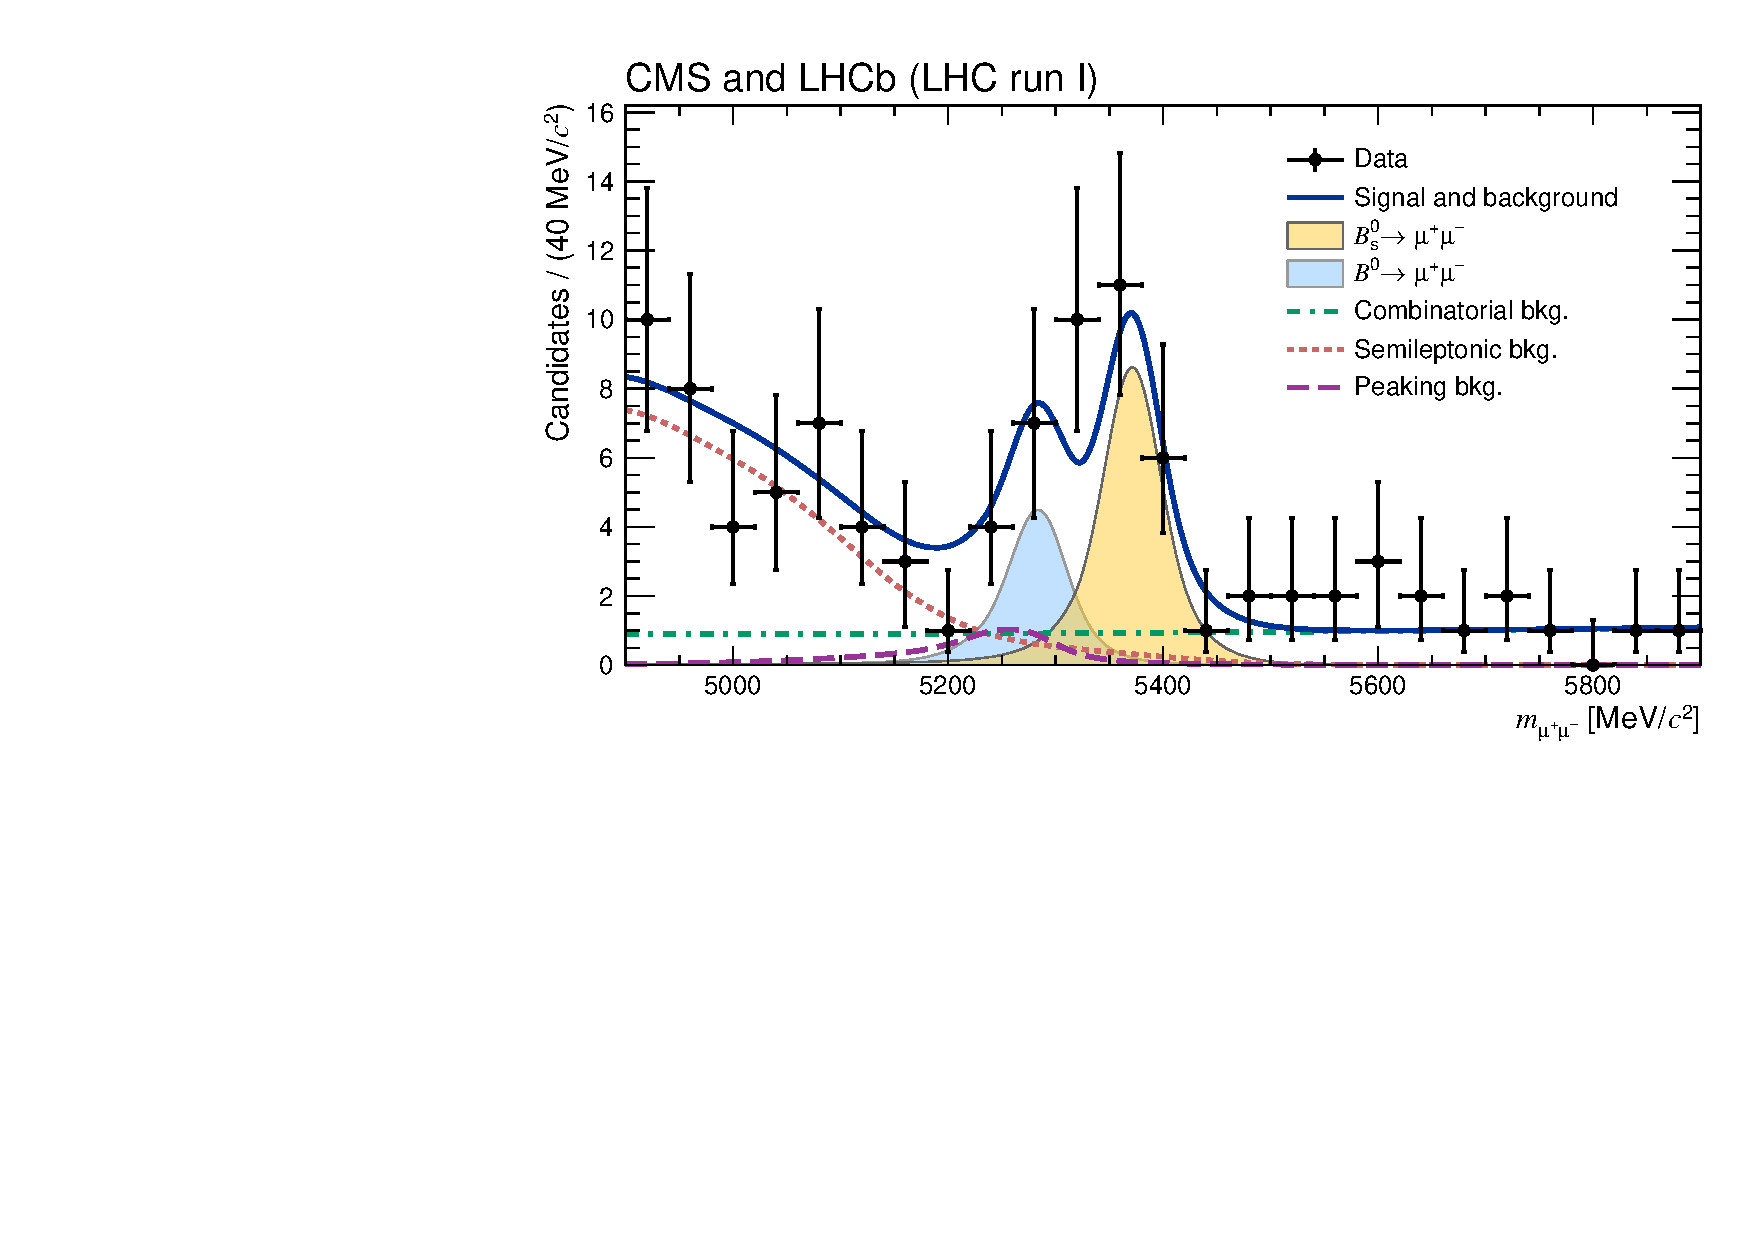
\includegraphics[width=0.6\textwidth]{Introduction/figs/CMSLHCb_EDfig2.pdf}
\caption{Dimuon invariant mass of $B$ candidates showing peaks corresponding 
$\Bs\to\mumu$ and $\Bz\to\mumu$ decays~\cite{CMS:2014xfa}.}
\label{fig:bsmumu}
\end{figure}

\subsection{Semileptonic $\bquark\to\squark\ell^+\ell^-$ decays of \bquark hadrons}
\label{sec:exp_btosll}

At the LHC it is possible to collect large data samples of semileptonic 
decays, especially those with muons in the final state.
Many branching fractions of semileptonic $B$ meson decays were recently measured at
the \lhcb experiment, including $\decay{B}{K\mumu}$, $\decay{B}{\Kstarz\mumu}$
and $\decay{\Bs}{\phi\mumu}$~\cite{LHCB-PAPER-2014-006,LHCB-PAPER-2013-017,LHCB-PAPER-2013-019}. 
Baryon decays were also studied at \lhcb: including 
the rare $\decay{\Lambda_b}{\Lz\mumu}$ decay~\cite{Aaij:2015xza}, whose analysis is described in this thesis.
In contrast to purely leptonic decays, SM predictions for semileptonic decays are affected by the
knowledge of hadronic form factors, which results in relatively large uncertainties,
$\mathcal{O}(30\%)$. As a result measurements are now typically more precise than predictions.

Among the measurements of angular observables that can be affected by 
new physics, particular interest was raised by a set of observables in $\decay{\Bz}{\Kstarz\mumu}$ 
decays, free from factors uncertainties at leading order~\cite{LHCB-PAPER-2013-037}.
Most of the measurements are found to be in agreement with SM predictions
with the exception of the $P'_{5}$ observable, shown in Fig.~\ref{fig:P5prime}, which presents
a local $3.7\sigma$ deviation confirmed by a recent LHCb analysis with higher 
statistics~\cite{Aaij:2015oid} and Belle~\cite{Abdesselam:2016llu}.
Attempts to build a consistent picture point to a new physics contribution
to the Wilson Coefficient $C_9$~\cite{Descotes-Genon:2013wba}.
An angular analysis of $\Bu\to K^+\mumu$ decays was also performed, where observables
are found to be compatible with SM predictions~\cite{LHCB-PAPER-2014-007}.
%
\begin{figure}[h!]
\centering
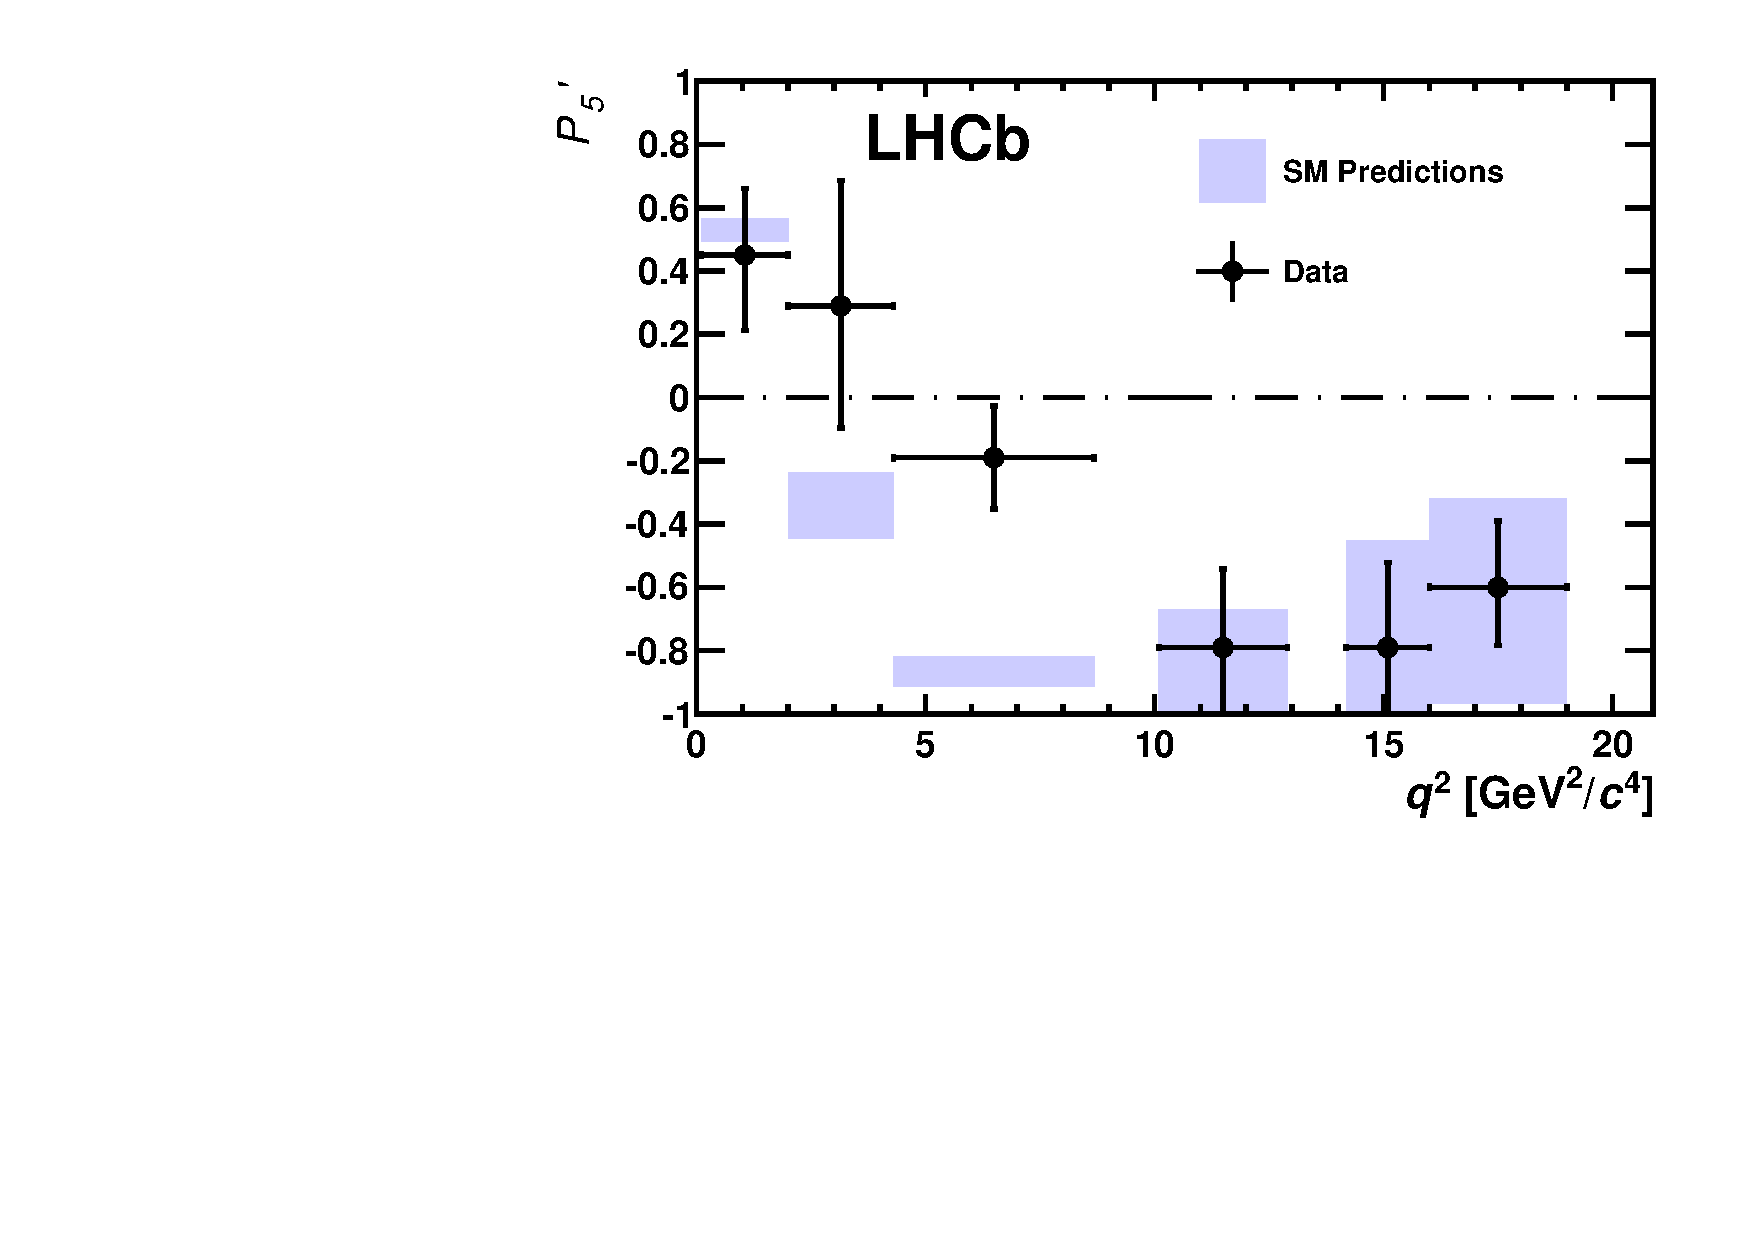
\includegraphics[width=0.6\textwidth]{Introduction/figs/P5prime.pdf}
\caption{Measurement of the $P'_{5}$ observable as a function of \qsq, showing a tension with
SM predictions in the 2--6 \gevgevcccc region~\cite{LHCB-PAPER-2013-037}.}
\label{fig:P5prime}
\end{figure}
%
Other observables for which the sensitivity to form factors effects is reduced are the CP asymmetry between
$B$ and $\bar{B}$ decays, $\mathcal{A}_{CP}$, and the isospin asymmetry between \Bz and \Bu decays, $\mathcal{A}_{CP}$.
Due to the small size of the corresponding CKM elements, CP asymmetries of $\Bz\to K^{(*)}\mumu$
decays are tiny in the SM, $O(10^{-3})$. In BSM models new sources of CP violation can arise and therefore
$\mathcal{A}_{CP}$ measurements are a powerful test of the SM. 
The isospin asymmetry is not zero in the SM due to isospin breaking effects in the form factors.
This is expected to be $\sim1$\% at low \qsq and increase to $\sim10$\% as \qsq tends to zero.
The LHCb experiment, using the full dataset collected in Run I, corresponding to an integrated luminosity of
3~\invfb and $\sim 10^9$ $B$ decays, measured both of these asymmetries to be consistent with
zero~\cite{LHCB-PAPER-2014-006,Aaij:2014bsa}, as reported in Tab.~\ref{tab:AcpAI}. 
%
\begin{table}
\begin{small}
\begin{tabular}{c|cc|cc}
\multirow{2}{*}{}	& \multicolumn{2}{c|}{$\Bz\to K^+\mumu$}			&\multicolumn{2}{c}{$\Bz\to \Kstarz\mumu$}	\\ \cline{2-5}
							& 1.1--6 	[\gevgevcccc]	& 15.0--22.0 [\gevgevcccc] & 	1.1--6 [\gevgevcccc]	& 15.0--19.0 [\gevgevcccc]			\\ \hline
$\mathcal{A}_{CP}$  & $0.004 \pm 0.028$	 				& $-0.005 \pm 0.030$		&	$0.094 \pm 0.047$	& $-0.074 \pm 0.044$ 	\\
$\mathcal{A}_{I}$	& $-0.10^{+0.08}_{-0.09} \pm 0.02$	& $-0.09 \pm 0.08 \pm 0.02$	&	$0.00^{+0.12}_{-0.10} \pm 0.02$  &	$0.06^{+0.10}_{-0.09} \pm 0.02$ \\
\end{tabular}
\end{small}
\caption{Measurement of CP and isospin asymmetry in $\Bz\to \Kstarz\mumu$ decays from the LHCb experiment~\cite{TomRDreview}.  }
\label{tab:AcpAI}
\end{table}
%
Recently, progress was also made measuring electron channels.
The branching fraction of the $\Bz\to\Kstarz\ee$ decay was measured to be $(3.1\pm1.3)\times10^{-7}$ in the dilepton mass interval 30--1000~\mevcc~\cite{LHCB-PAPER-2013-005}. Furthermore, for the first time
angular observables were measured for this decay and found to be consistent with SM predictions~\cite{Aaij:1981106}.

Given the wide set of available measurements, theorists have implemented global fits including results from rare decays analyses,
 as well as inputs from \Bs mixing and Higgs measurements, in order to understand if the existing anomalies could be caused by a common factor.
The results of such global fits agree that there is a tension with respect to the SM at the level of 3--4 standard deviations,
depending on the set of assumptions made. In particular they favour a shift $C^{NP} \sim -1$ to the $C_9$ Wilson
Coefficient, related with the penguin diagram mediated by a $Z^0$ boson~\cite{Altmannshofer:2014rta,Descotes-Genon:2013wba,Hurth:2016fbr}. 

\subsection{Lepton Flavour Violation searches}

Several Lepton Flavour Violation (LFV) searches are linked to rare decays as they involve small branching
ratios in the SM that can be enhanced by BSM physics. %They are therefore a natural place to look for new physics.
Lepton flavour conservation is experimentally well-established measuring the branching ratios of
decays of muons into electrons and no neutrinos, but has no strong theoretical
explanation in the context of the SM. In fact it is already observed that flavour
is not conserved in neutrino oscillations. 
%This section reports a short review of LFV searches. 
%
The best-studied decays violating lepton flavour 
are rare muon decays including $\mu^+\to e^+\gamma$ and $\mu^+\to e^+e^-e^+$.
Since muons can be abundantly produced and the final states are simple,
these decays provide the best constraints to LFV. The current best upper limits are $1.2 \times 10^{-11}$
for the radiative decay and $1.0 \times 10^{-12}$ for \mbox{$\mu^+\to e^+e^-e^+$} obtained
respectively by the MEGA~\cite{Ahmed:2001eh} and SINDRUM~\cite{Bellgardt:1987du} experiments.
Several LFV searches in the $B$ sector have recently been performed at the LHCb experiment 
including decays such as $\Bz\to e\mu$~\cite{LHCB-PAPER-2013-030} and $\tau$ decays such
as $\tau\to\mumu\mu$~\cite{LHCB-PAPER-2013-014}. None of these searches has found evidence 
of new physics so far and therefore they set limits, constraining the parameter space available for BSM models.
Figure~\ref{fig:LFV_decay} shows a summary of the best limits set at different times
on LFV searches~\cite{Marciano:2008zz}.


\begin{figure}[h!]
\centering 
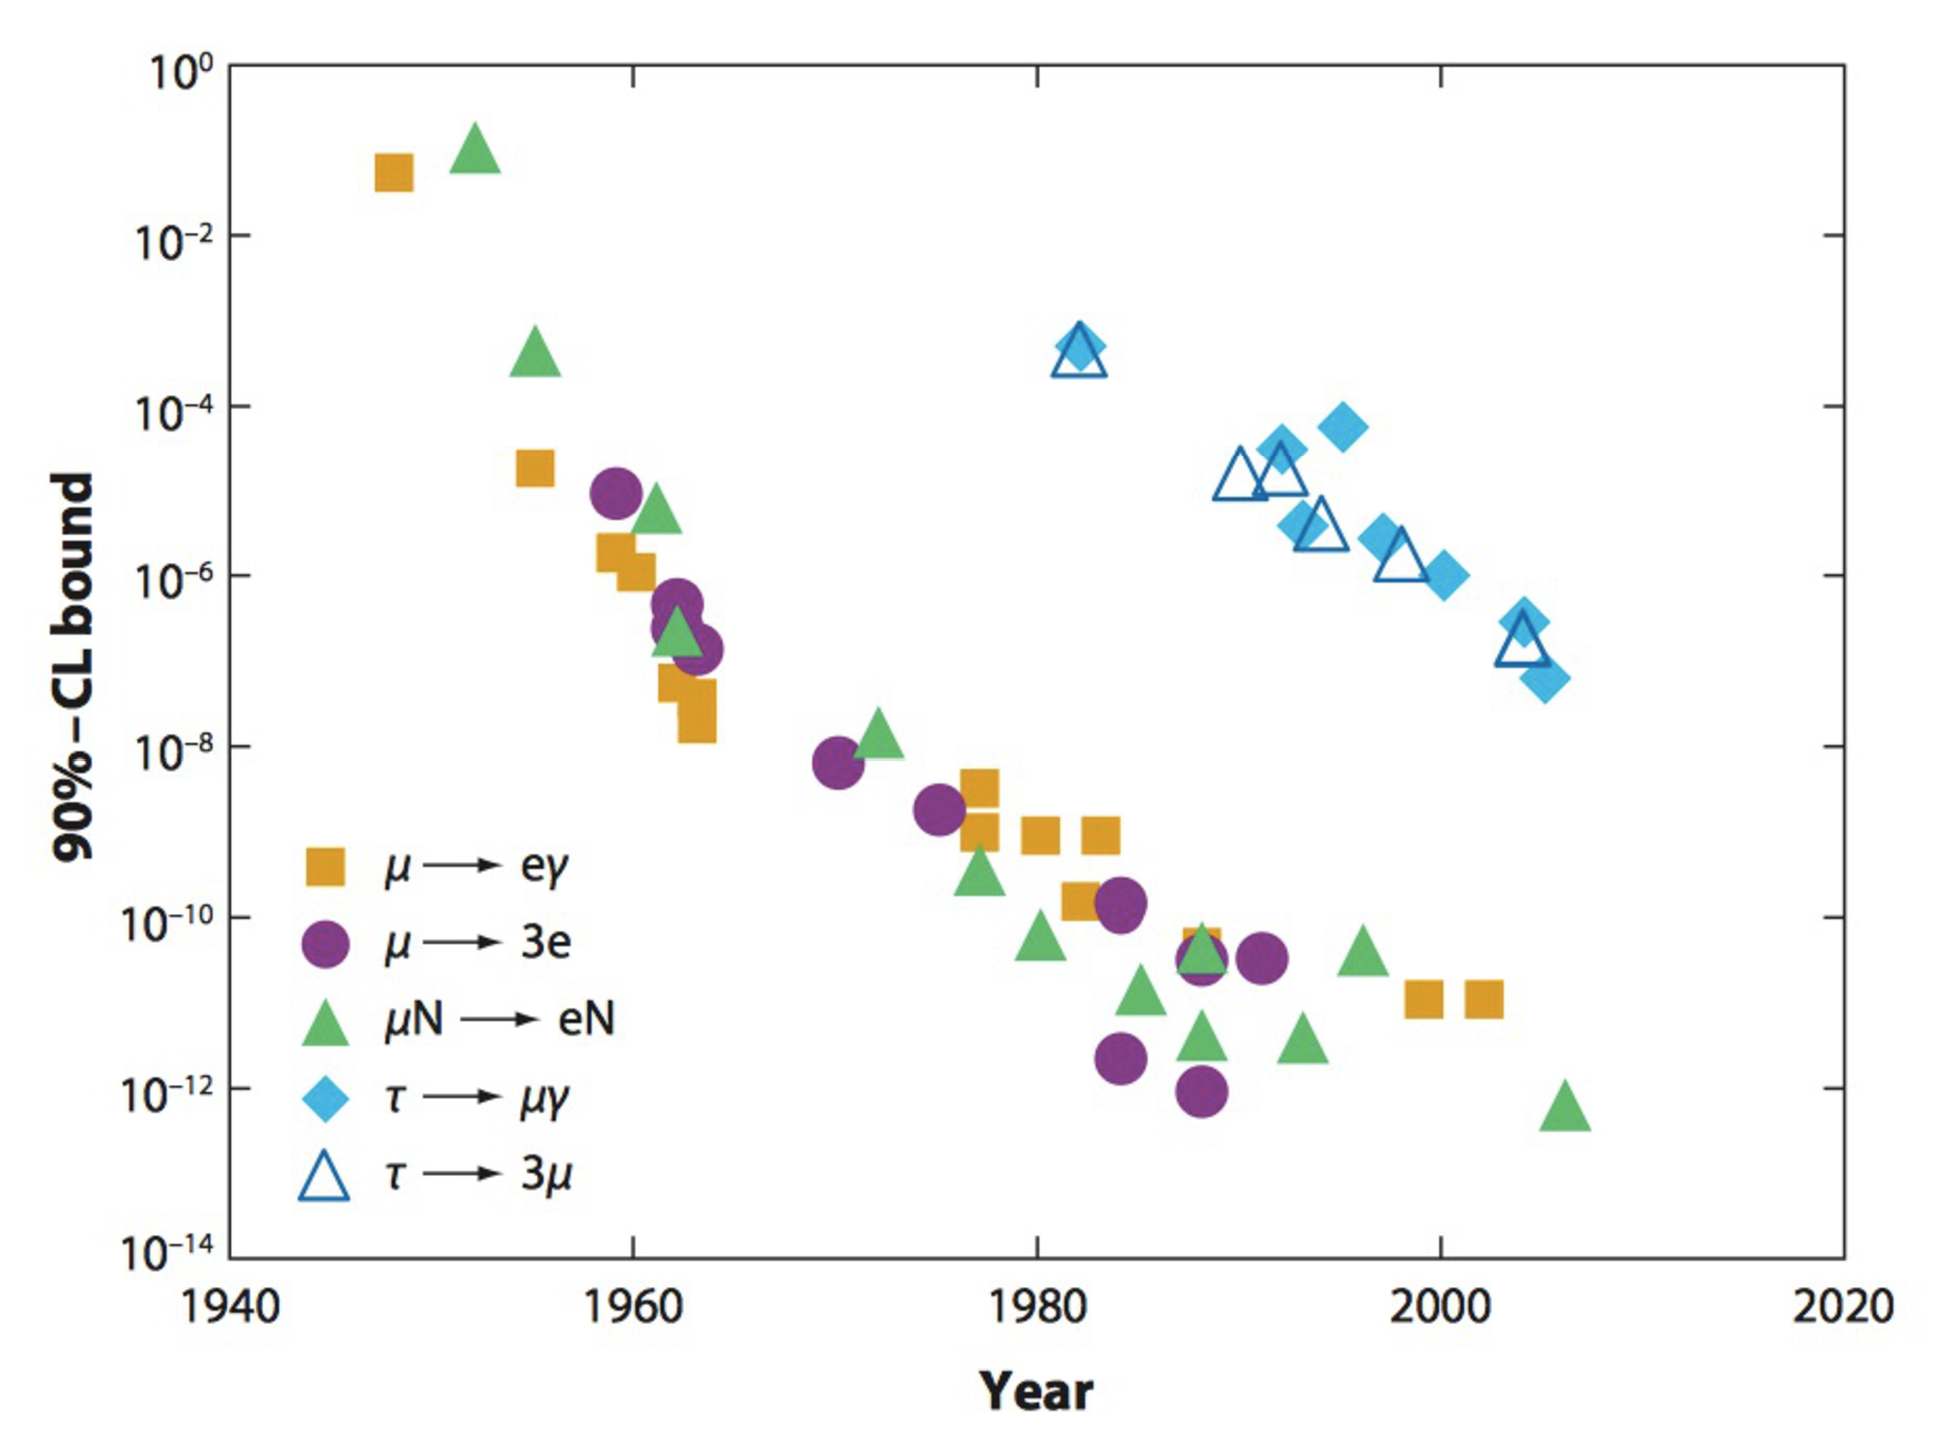
\includegraphics[width=0.7\textwidth]{Introduction/figs/LFV.pdf}
\caption{Summary of limits set in LFV searches as a function of time~\cite{Marciano:2008zz}.}
\label{fig:LFV_decay}
\end{figure}
 


\chapter{The LHCb detector at the Large Hadron Collider}
\label{sec:Detector}

\section{The Large Hadron Collider}

The Large Hadron Collider (LHC) is a circular particle accelerator with a circumference of 27 km about 100 m underground.
The two general-purpose detectors, ATLAS and CMS, sit on opposites sides of the ring, while the two smaller specialty detectors, 
ALICE and LHCb, are at the interaction points to either side of ATLAS (see fig. \ref{lhc}).

\begin{figure}[h!]
\centering
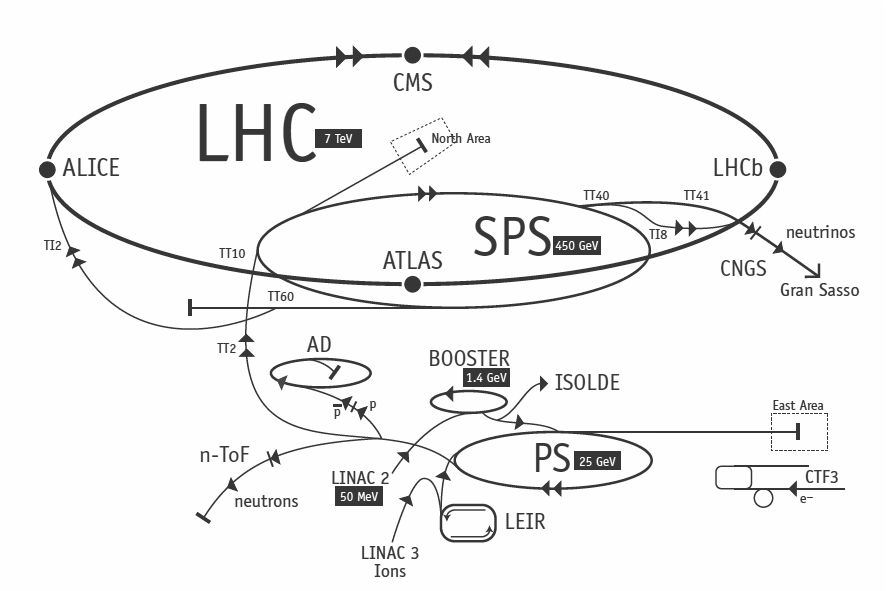
\includegraphics[width=1\textwidth]{Detector/figs/LHC_scheme.png}
\caption{Scheme of CERN accelerators.} \label{lhc}
\end{figure}

Two proton beams circulate in opposite directions around the ring and cross each other at several points, 
in which are placed huge particle detectors. Each beam consists of a series of proton bunches, up to a maximum of 2835
in the beam. Each bunch consists of about $10^{11}$ protons and the bunch spacing is such that the nominal bunch crossing
rate is 40 MHz. The beams are injected into pre-accelerators and then led into LHC through the CERN acceleration
system shown in figure \ref{lhc}. Protons are produced from duoplasmatron, starting from hydrogen gas, and are
initially accelerated to the energy of 50 MeV in a linear accelerator (LINAC). Then, protons are injected into
the Proton Synchrotron Booster (PSB) where they are boosted to an energy of 1.4 \gev, then into the Proton Synchrotron (PS)
to 25 GeV and Super Proton Synchrotron (SPS) to 450 GeV. Finally, protons enter into the LHC storage ring.
In the main ring proton beams are accelerated from injection energy to the final one by radio frequency (RF) cavities.
The beams are steered around the ring by 8 T magnetic fields produced in 15 meter long superconducting niobium-titanium
dipole magnets, and focused by quadrupole and multipole magnets. The LHC magnets use a design in which both proton beam
pipes are contained in the same housing, allowing the same liquid helium to cool the system down for both \cite{lhc}.
The LHC began colliding proton beams in physics mode in 2009 at and energy of $\sqrt{s} = 900$ GeV and from April 2010
to November 2011 accelerated beams at $\sqrt{s} = 7$ TeV (3.5 TeV per proton beam). At this energy it delivered over
$5.7 \text{ fb}^{-1}$ of collisions, with a maximum instantaneous luminosity of $3\cdot10^{33} \text{ cm}^{-2}\text{s}^{-1}$.
The LHC maximum design energy is 14 TeV, and its design luminosity is $10^{34} \text{ cm}^{-2}\text{s}^{-1}$.
After a long shut down to upgrade and maintain the machine, a new run started in June 2015 where protons
are collided at an energy of $\sqrt{s} = 13$ \tev at this energy the total proton-proton cross section
is expected to be roughly 100 mb.
%, thus at the design luminosity the general purpose detectors will an event rate approximately $10^9$ inelastic events/s.

\section{The LHCb detector}

The LHCb detector was built with the main purpose of studying the decays of B and D mesons, looking in particular for CP-violating processes. In 2011, running at a centre of mass energy of 7 TeV, the cross section of $b\bar{b}$ production was measured to be $284 \pm 53 ~\mu b$\cite{Aaij:2010gn}, while it will be $\sim500 ~\mu b$ at the nominal LHC energy, 14 TeV.
At these high energies, proton-proton interactions produce highly boosted virtual gluons which interact to produce $b\bar{b}$ pairs at small angles, close to the beam pipe. For this reason the LHCb detector is designed to have a very forward angular coverage: it is fully instrumented from approximately 10 mrad to 300 mrad, corresponding to $2 < \eta < 5$, where $\eta$ is a quantity used in particle physics and called ``pseudorapidity" and defined as:
\begin{equation}
\label{pseudorap}
\eta = - \ln(\tan(\theta/2))
\end{equation}
In Eq. \ref{pseudorap}, $\theta$ is the angle between a particle's momentum and the beam direction\footnote{LHCb's reference system has the $z$ axis in the direction of the beam, the $x$ axis directed to the centre of the accelerator and $y$ is directed upward. Then we define $\theta$ as the angle with the beam direction and $\phi$ as the position around the beam in the $xy$ plane, taking $\phi = 0$ on the $x$ axis.}.

\begin{figure}[h]
\label{lhcb}
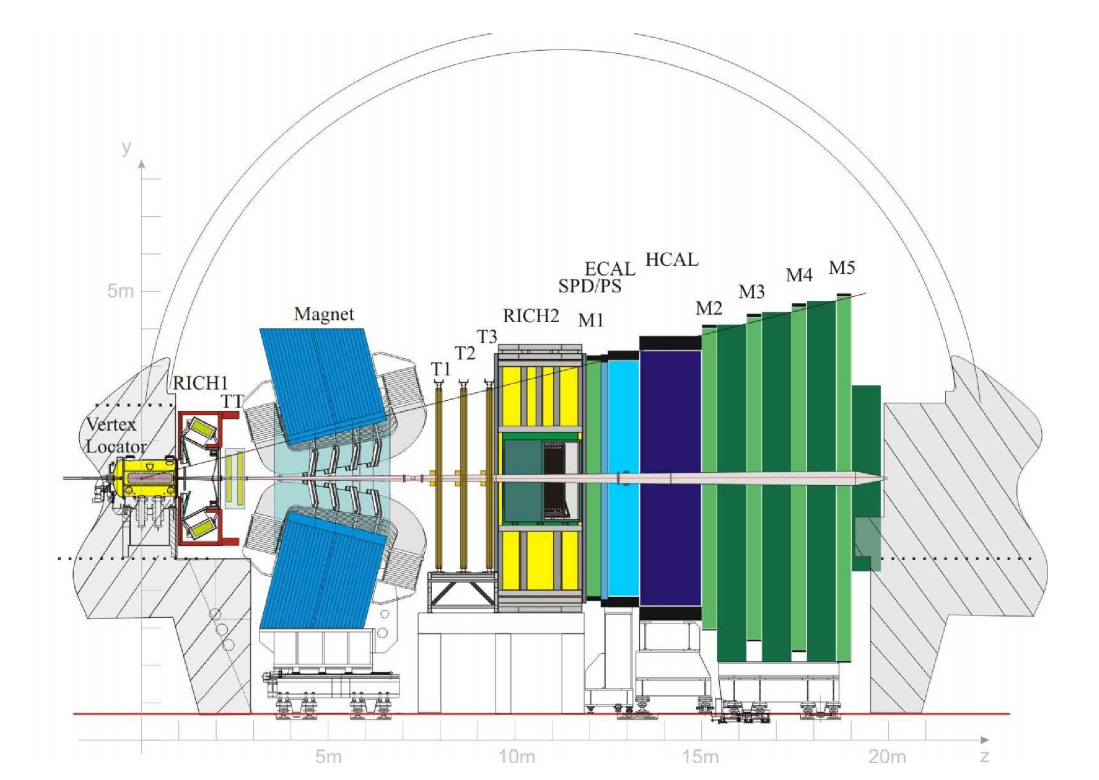
\includegraphics[width=0.9\linewidth]{Detector/figs/LHCb_official.png}
\caption{A side view of the LHCb detector \cite{Alves:2008zz}.}
\end{figure}

At the collision point of LHCb the luminosity can be adjusted by displacing the beams from head on collisions while keeping the same
crossing angle. This allows the experiment to keep an approximately constant instantaneous luminosity. This also means that the average number of interactions per bunch crossing can be limited as LHCb efficiency, especially of detecting secondary vertices, decreases for events with an high number of primary vertices (PV). Reducing the particle occupancy through the detector also keeps radiation damage to a minimum. Since the LHC started colliding protons in
November 2009 until the end of 2011, the instantaneous luminosity was at an average of $3 \cdot 10^{32} \mbox{cm}^{-2}\mbox{s}^{-1}$, with an average number of 1.5 vertices per bunch crossing in LHCb. At the end of 2011 LHCb had collected an integrated luminosity of $1 ~\mbox{fb}^{-1}$; in 2012 the luminosity was increased and $2 ~\mbox{fb}^{-1}$ more were collected.

Other B physics experiments, like BaBar at the Stanford Linear Accelerator (SLAC), Belle at KEK at J-PARC (Japan) and the Tevatron experiments at Fermilab have made accurate measurements in heavy flavour physics. All of these results have so far been consistent with the Standard Model predictions. However, some of the deviations from the Standard Model are expected to be very small, therefore LHCb has begun to make the most precise measurements in heavy flavour physics.

The LHCb detector\cite{Alves:2008zz} includes a high-precision tracking system consisting of a silicon-strip vertex detector surrounding the $pp$ interaction region, a large-area silicon-strip detector located upstream of a dipole magnet with a bending power of about 4 Tm, and three stations of silicon-strip detectors and straw drift tubes placed downstream. The combined tracking system has momentum resolution $\Delta p/p$, that varies from 0.4\% at 5 $\mbox{GeV/c}^{2}$ to 0.6\% at 100 $\mbox{GeV/c}^{2}$.
Charged hadrons are identified using two Ring-Imaging Cherenkov detectors (RICH)\cite{LHCb-DP-2012-003}. Photon, electron and hadron candidates are identified by a calorimeter system consisting of scintillating-pad and pre-shower detectors, an electromagnetic calorimeter and a hadronic calorimeter. Muons are identified by a system composed of alternating layers of iron and multiwire proportional chambers\cite{LHCb-DP-2012-002}. A schematic view of the detector is shown in Fig. \ref{lhcb}.


\subsection{Tracking system}

The tracking system is made up of the Vertex Locator (VeLo), and 4 tracking stations: the Tracker Turicensis (TT) which are located before the magnet and T1, T2 and T3 which are downstream of the magnet. Charged particle tracks are bent horizontally in the magnetic field so that their momentum can be measured from the curvature radius.

B mesons have lifetimes of approximately 1.5 ps. At the LHC energies, this means they travel about 1 cm before decaying and they form a displaced vertex. It is therefore important to be able to separate the particles produced at the primary $p-p$ vertex and the B decay vertex.

The VeLo accurately measures positions of tracks close to the interaction point so that production and decay vertices of bottom and charm hadrons can be reconstructed. The VeLo is made up of 21 staggered silicon modules which surround the beam axis and are positioned from $z = -18$ cm to $+80$ cm. It is able to detect particles within a pseudorapidity range $1.6 < \eta < 4.9$. The sensitive region of the VeLo starts at an inner diameter of 8mm from the beam axis. The VeLo is housed in its own vacuum vessel of thin aluminium foil which protects the vacuum of the beam pipe from any outgassing of the VeLo. VeLo stations consist of two modules, and each has two types of sensors: the $\phi$-sensor which measures the azimuthal position around the beam, and the R-sensor which measures the radial distance from the beam axis. A sketch of the VeLo sensor is shown in Fig. \ref{VeLo}. The sensors are 300 $\mu m$ thick, approximately semicircular and are positioned on either side of the beam axis. To ensure that they cover the full azimuthal angle the right-side module is placed 1.5 cm behind the left-side module on the z-axis and they overlap. There are two modules which cover the backward direction and were used as a veto for multiple interactions in 2011, called the pileup veto.

\begin{center}
\begin{figure}[h!]
\label{VeLo}

\begin{minipage}{0.49\textwidth}

\centering 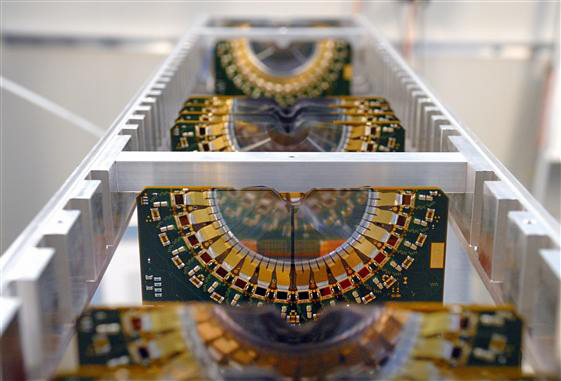
\includegraphics[width=0.8\textwidth]{Detector/figs/detector/VELO.png}

\end{minipage}
\begin{minipage}{0.49\textwidth}

\centering 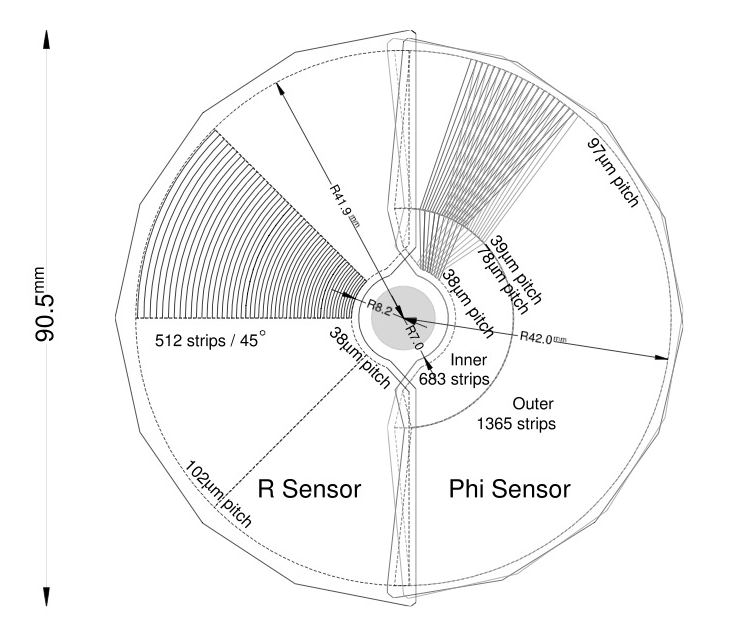
\includegraphics[width=0.8\textwidth]{Detector/figs/detector/VELO_scheme.png}

\end{minipage}
\caption{On the left VeLo sensors mounted in line and on the right a schematic view of one sensor \cite{Alves:2008zz}.}
\end{figure}
\end{center}

The LHCb dipole magnet is comprised of two coils supported on an iron yoke and is wedge-shaped to fit the LHCb 
angular acceptance. It is a warm magnet so can be ramped easily and the field can be reversed periodically. 
This is used to limit some systematics that can arise form imperfections performance in different areas of the detector.

The IT and TT both use silicon microstrip and together constitute the Silicon Tracker (ST). Straw tubes are used 
in the outer regions of the tracking stations which together are called the Outer Tracker (OT). The IT has 
an higher inner granularity because of the higher flux of particles nearer the beam pipe. Each ST station 
has four detection layers, the first and last being vertical, measuring the track position in x. The second 
and third layer are rotated by a stereo angle of +5 and -5 degrees, which allows the y-coordinate to be measured. 
The TT is placed upstream of the magnet which allows reconstruction of the tracks from low-momentum particles which 
are swept out of the downstream acceptance.

\subsection{Particle identification}

Particle identification in LHCb is performed in various ways. The calorimeter detects particles with high 
transverse momentum, the muon chambers identify muons and the Ring Imaging Cherenkov (RICH) detectors identify 
heavier charged particles.

\subsubsection{Calorimeters}
\label{sec:calorimeters}

The main purpose of the calorimeter system is to determine the energy of particles traversing the detector. 
The material in the calorimeter system is layered with absorber and active material. The absorber makes particles
interact and produces a cascade of secondaries, which multiply quickly and are detected by the active part. 
The sensitive material consists of scintillating layers, where the light detected is approximately proportional 
to the number of deposited particles. Calibration is then used to calculate the deposited energy. The calorimeter 
system is essential for flavour tagging because it identifies electrons. In addition, it is required for accurately 
reconstructing
$\pi^0$ particles and prompt photons, which are both needed for the study of B-meson decays. The LHCb calorimeter 
system consists of the Scintillator Pad Detector (SPD), the Pre-Shower Detector (PS) as well as the Electromagnetic 
Calorimeter (ECAL) and the Hadronic Calorimeter (HCAL). All four detectors transmit scintillation light via 
wavelength-shifting fibres to photo-multiplier tubes (PMTs). The SPD/PS cells are read out with MAPMTs 
(Multi-anode PMTs) located outside the LHCb acceptance. The ECAL and HCAL have individual MAPMTs located on the modules.
All four detectors vary the segmentation of their cells according to the distance from the beam pipe.
The purpose of the SPD and PS is to separate the electrons from a high background of neutral and charged pions 
produced in the collisions. In order to obtain the highest energy resolution the showers from high energy photons 
must be fully absorbed. For this reason the ECAL has a thickness of 25 radiation lengths and its resolution is 
measured to be \cite{Alves:2008zz}
 
 \begin{equation}
 \frac{\sigma_{ECAL}(E)}{E} = \frac{10\%}{\sqrt{E(GeV)}} + 1\%
 \end{equation}

The trigger requirements on the HCAL resolution do not depend on the containment of the hadron showers as much 
as for the ECAL, so due to a limited space, its thickness is only 5.6 interaction lengths and its resolution

 \begin{equation}
 \frac{\sigma_{HCAL}(E)}{E} = \frac{69\%}{\sqrt{E(GeV)}} + 9\%
 \end{equation}




\subsubsection{RICH}

The two RICH detectors are a special feature of LHCb, as it is the only experiment at LHC including them. 
These detectors take advantage of the  Cherenkov light produced by particles passing in a medium with velocity 
higher that the velocity of light in the medium. The Cherenkov light, as shown in Fig. \ref{Cherenkov}, 
is produced in cones with a specific angle depending on the velocity of the particle

\begin{equation}
cos(\theta) = \frac{1}{\beta n}
\end{equation}

where $\beta$ is the velocity of the particle over $c$ and $n$ is the refraction index of the medium.

\begin{center}
\begin{figure}[h!]
\label{Cherenkov}

\begin{minipage}{0.45\textwidth}

\centering 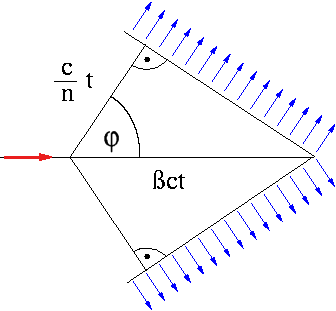
\includegraphics[width=0.8\textwidth]{Detector/figs/detector/Cherenkov.png}

\end{minipage}
\begin{minipage}{0.55\textwidth}

\centering 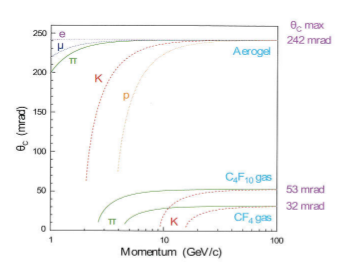
\includegraphics[width=0.8\textwidth]{Detector/figs/detector/RICH_performance.png}

\end{minipage}
\caption{On the left a sketch of Cherenkov light emission \cite{wikiCherenkov} and on the right the Cherenkov
angle versus momentum for the two radiators of RICH1 and for different particles. One can see that they allow
to separate particles in different momentum ranges.}
\end{figure}
\end{center}

RICH 1 is situated before the magnet in order to cover a large angular acceptance. Its purpose is to ensure
particle identification over the momentum range $1 < p < 70$ GeV. It uses two radiators, $C_4F_{10}$ covers
the momentum range $5 - 70$ GeV/c, and silica aerogel which covers $1 - 10$ GeV/c. RICH 2 is situated after
the magnet and tracking stations. It identifies higher momentum particles from approximately 20 GeV up to beyond
100 GeV using $CF_4$ as a radiator.
The Cherenkov light produced when charged particles travel through the radiators, is reflected and focused using
flat and spherical mirrors which are tilted so that the ring image is reflected onto arrays of photo-detectors.
The radius of the ring becomes equivalent to the opening angle of the Cherenkov cone because of the known geometry.
The photo-detectors are located outside of the LHCb acceptance in order to reduce the amount of material that
the particles have to traverse. Pattern recognition algorithms are then used to reconstruct the Cherenkov rings.

For particle identification a particle type hypothesis is assigned to each charged track found in the tracking stations.
Initially the hypothesis is for a pion, which is the most common particle type. The corresponding expected number and
Cherenkov radii of the resulting photons are calculated and the likelihood is calculated. The hypothesis is then changed
and the likelihood is recalculated. The case with the largest increase in likelihood is kept.


\subsection{The muon system}

\begin{figure}[b!]
\label{muonsystem}
\centering 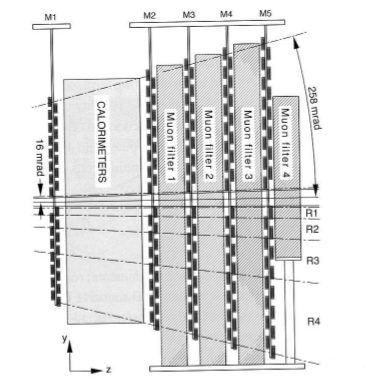
\includegraphics[width=0.5\linewidth]{Detector/figs/muonsystem.png}
\caption{The LHCb muon system \cite{Alves:2008zz}.}
\end{figure}

It is essential for many of the key physics analyses to be able to identify muons in the final state.
Muons are the most penetrating particles that can be detected at LHC experiments, so the muon chambers
are the final subdetectors. There are five stations (M1 - M5), the first one being located before the calorimeter
in order to improve the $p_T$ measurements. A scheme of the muon system is shown in Fig. \ref{muonsystem}.

The remaining four lay behind the HCAL and are separated by 1.2 m from each other, interleaved with iron block
filters 80cm thick, which absorb hadrons, electrons and photons to ensure that only muons reach the final muon station.
Only muons with a minimum momentum of 10 GeV/c traverse all of the five stations and for positive identification of a muon
the trigger requires a signal in each of them. Each station has a detection efficiency of at least 95\% and the detectors
provide position measurements. Since there is a larger particle flux towards the beam pipe, the stations are divided
into four concentric rectangular regions (R1-R4), their size increasing according to the ratio 1 : 2 : 4 : 8.
This means that there is a similar channel occupancy over the four regions. All of the muon stations use
Multi Wire Proportional Chambers (MWPC) except for the inner region of M1, where the particle flux is too high.
In this region triple-GEM (Gas Electron Multiplier) detectors are used instead because they have better ageing properties.

The Gas Electron Multiplier (GEM) detectors in the inner region of M1 have to  withstand a rate up to
$500 ~\mbox{kHz cm}^{-2}$ of charged particles. Particles traversing through the drift gap between the cathode
and the first GEM foil produce ionisation electrons which are then attracted by electric fields though all of the
GEM foils and they multiply. They then drift into the anode inducing a signal on the pads. A gas mixture of Argon,
$CO_2$ and $CF_4$, is used to give a time resolution better than 3 ns.




\subsection{Trigger and software}

The LHCb trigger system\cite{LHCb-DP-2012-004} consists of a hardware stage (L0), based on information from the calorimeter
and muon systems, followed by a software stage (HLT), which applies a full event reconstruction. To increase performances
the HLT is split again into stages (HLT1 and HLT2). The bunch crossing frequency is $40 ~\mbox{MHz}$, which corresponds
to an instantaneous luminosity of $2 \cdot 10^{32} ~\mbox{cm}^{-2} \mbox{s}^{-1}$ for LHCb, and about 15\% of the total
number of $b\bar{b}$ pairs produced will have at least one B meson with all of its decay products within the detector acceptance.
This needs to be reduced down to about 2 kHz so that the events can be written to disk for analysis. Fig. \ref{triggerscheme}
shows a scheme of the trigger system.

The L0 reduces the rate of visible interactions from 10 MHz to a rate of 1 MHz and uses mainly the information from the 
calorimeter dividing the events in the 5 categories: L0Photon, L0Electron, L0LocalPion, L0GlobalPion, L0Hadron. ``local" pions
refer to $\pi^0$ reconstructed though decay in $\gamma\gamma$, where the two photons fall in the same ECAL board, they are
labelled ``global" otherwise. The HLT1 uses information from the VELO and trackers performing a partial reconstruction
of the event and reduces the rate to 2 kHz. Finally the HLT2 involves a full reconstruction of the event and includes many
``lines" designed to trigger specific decays.

LHCb also developed an extended simulation software in order to reconstruct efficiencies and signal shapes.
In the simulation, $pp$ collisions are generated using $\textsc{Pythia}$~6.4\cite{Sjostrand:2006za} with a specific
LHCb configuration\cite{LHCb-PROC-2010-056}. Decays of hadronic particles are described by $\textsc{EvtGen}$\cite{Lange:2001uf},
in which final state radiation is generated using $\textsc{Photos}$\cite{Golonka:2005pn}. The interaction of the generated
particles with the detector and its response are implemented using the $\textsc{Geant4}$ toolkit\cite{Allison:2006ve, *Agostinelli:2002hh}
as described in \cite{LHCb-PROC-2011-006}.

For the analysis in this document, I used the ROOT framework\cite{Brun:2000es} to analyse data, the RooFit package
fot fitting. The multivariate analysis is base on ne NeuroBayes package \cite{} which provides a framework
for neural network training.

\begin{figure}[t!]
\label{triggerscheme}
\centering 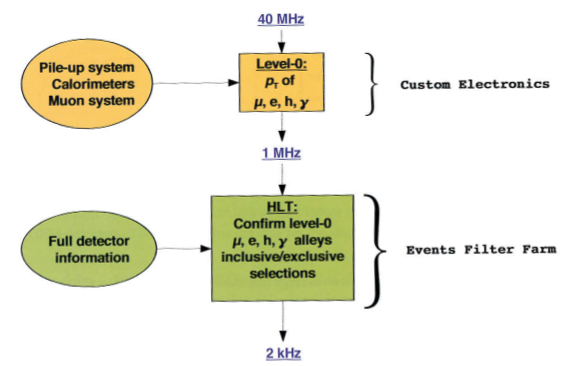
\includegraphics[width=0.8\linewidth]{Detector/figs/triggerscheme.png}
\caption{Scheme of the LHCb trigger system \cite{Alves:2008zz}.}
\end{figure}







%%%%%%%%%%%%%  Lb->Lmumu
\part{Differential branching fraction and angular analysis of the rare \Lb\to\Lz\mumu decay}
\label{par:Lmumu}
%\chapter{Differential branching fraction of the rare \Lb\to\Lz\mumu decay}
\chapter{Differential branching fraction of $\protect\Lb\to\Lz\mumu$}
\label{sec:Lmumu_intro}

The rare $\Lb\to\Lz\mumu$ decay is a FCNC process governed by the $\bquark \to \squark\mumu$ quark
level transition. In the SM this decay proceeds only through loop diagrams, electroweak penguin and \W box
(see Fig.~\ref{fig:penguins}), and therefore it is highly sensitive to new particles entering the loops. 
%Moreover, as the final state contains only a single long-lived hadron,
%the hadronic physics is easier to handle than in fully hadronic decays.
%\begin{figure}[hbt]
%\centering
%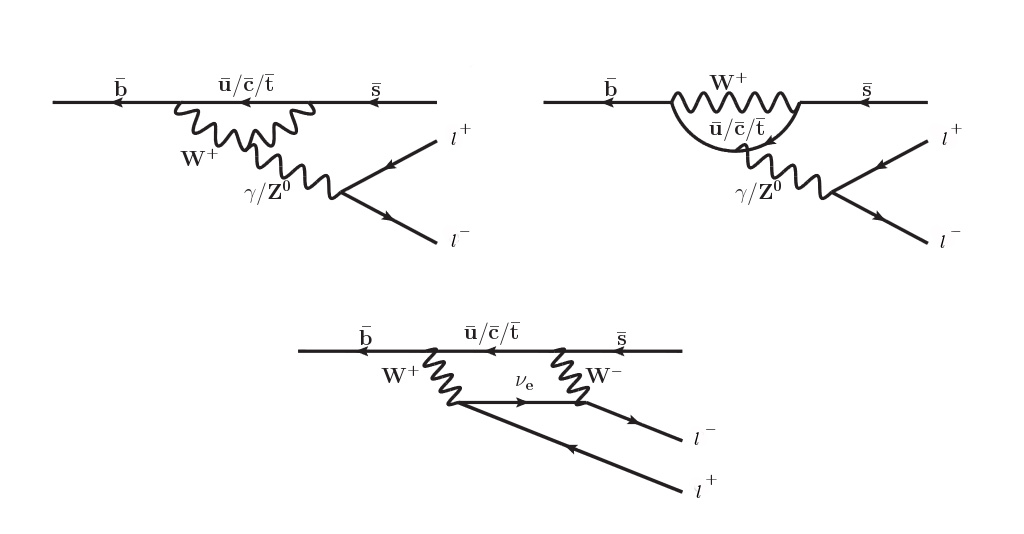
\includegraphics[width=0.8\textwidth]{Lmumu/figs/penguins3.png}
%\caption{Loop Feynmann diagrams for the rare $b \rightarrow s $ decay.}
%\label{fig:penguins}
%\end{figure}
%
Interest in \Lb baryon decays arises from two important facts.
First of all, \Lb has non-zero initial spin, which allows to learn information about the helicity structure
of the underlying Hamiltonian, that cannot be extracted from the meson decays~\cite{Hiller:2007ur,Mannel:1997xy}.
Secondly, the \Lb baryon can be considered in first approximation as composed of an heavy 
quark and a light di-quark, therefore the hadronic physics significantly differs from similar meson decays.
This provides the possibility to better understand and test the hadronic physics in the theory,
which could yield improved understanding and confidence also for the meson case.

With respect to \Bz decays going though the same transitions, such as \BdToKstmm, \Lb decays can provide independent
confirmations of the results as they involve the same operators but different hadronic matrix elements.
Furthermore, \Lz decays weakly, which results in complementary constraints with respect to \Bz decays.
Finally, the narrow width approximation, used in theoretical calculations, is fully applicable in the \Lb case,
which has $\Gamma_{\Lb} \sim 2.5 \cdot 10^{-6}$ \ev. This is not assured for \BdToKstmm decays because
the contribution from the non resonant channel $\decay{\Bz}{K\pi\mumu}$ is unconstrained.

The theory of the $\Lb\to\Lz\mumu$ decays was considered by a number of authors both in the SM and in different
new physics scenarios~\cite{Aslam:2008hp,Wang:2008sm,Huang:1998ek,Chen:2001ki,Chen:2001zc,Chen:2001sj,
Zolfagharpour:2007eh,Mott:2011cx,Aliev:2010uy,Mohanta:2010eb,Sahoo:2011yb}.
All authors start from the same effective Hamiltonian already described in Sec.~\ref{sec:Effective_Hamiltonian}. 
However, form factors, describing hadronic physics, are not developed as well as for the meson case 
because there are not as many experimental constraints. This leads to a relatively
large spread in predicted branching fractions. For these reasons an interesting quantity to study is the differential 
branching fraction as function of \qsq. This still suffers from the knowledge of form factors, but, as different 
approaches to form factors calculations are applicable in different \qsq regions, it allows a more meaningful comparison with theory.

Experimentally, the decay $\Lb\to\Lz\mumu$ was observed for the first time in 2011 by the CDF 
collaboration~\cite{Aaltonen:2011qs}, with a signal yield of $24\pm5$ events and was later updated using
their full statistics~\cite{Behari:2013xc}. CDF observed the signal only in the \qsq region above the square of the \psitwos mass.
Their result on full statistics yields $\mathcal{B}($\Lb\to\Lz\mumu$) =[1.95\pm0.34(\mathrm{stat})\pm0.61(\mathrm{syst})]\times 10^{-6}$.
Recently, the decay was also observed at LHCb~\cite{LHCb-PAPER-2013-025} with a yield of $78\pm12$ signal events
using 1~\invfb of integrated luminosity collected in 2011. The signal was again found only in the high \qsq region, above $m^2_{\psitwos}$.
The LHCb result for the branching fraction relative to the $J/\psi\Lambda$ decay, used as normalisation channel, is 
%
\begin{equation*}
\frac{\mathcal{B}(\Lb\to\Lz\mumu)}{\mathcal{B}(\Lb\to\jpsi\Lz)}=[1.54 \pm 0.30 ~(\mathrm{stat})~ \pm 0.20 ~(\mathrm{syst})~ \pm 0.02 ~(\mathrm{norm})]\times 10^{-3} 
\end{equation*}
and for absolute branching fraction
\begin{equation*}
\mathcal{B}(\Lb\to\Lz\mumu) =[0.96 \pm 0.16 ~(\mathrm{stat})~ \pm 0.13 ~(\mathrm{syst})~ \pm 0.21 ~(\mathrm{norm})]\times 10^{-6}.
\end{equation*}

This chapter describes the measurement of the differential branching fraction
of the $\Lb\to\Lz\mumu$ decay using 3~\invfb of $pp$ collisions collected by the LHCb experiment in 2011 and 2012.
Furthermore, in the next chapter an angular analysis of these decays is performed for the first time, measuring observables
including the forward-backward asymmetries in the leptonic and hadronic systems.

\section{Analysis strategy and \qsq regions}
\label{sec:Lb_q2choice}

A typical \qsq spectrum of $\bquark\to\squark\ll$ decays was shown in Fig.~\ref{fig:q2spectrum}.
This is characterised by the presence of the photon pole at low \qsq and the narrow peaks of the \jpsi and \psitwos resonances at mid \qsq.
For this analysis two regions are defined: the ``low \qsq" region, below the \jpsi resonance ($\qsq < 8$ \gevgevcccc),
where the signal is unobserved, and the ``high \qsq" region, above the \jpsi resonance ($\qsq > 11$ \gevgevcccc).
The decay $\Lb\to\jpsi\Lz$, where \jpsi decays into two muons has the same final state as the signal and
is used as a normalisation channel.
% and the branching fraction measurement is given in relative form to limit systematic uncertainties. 
In both cases the \Lz decay mode into a pion and a proton, $\Lz\to p\pi$,
is used to reconstruct the decays. The rare and normalisation channels are naturally distinguished
by the \qsq interval they fall into. The regions in which the rare channel is studied include:
\begin{itemize}
\item $0.1 < \qsq < 8$ \gevgevcccc, where the selection is optimised to observe the signal as explained in Sec.~\ref{sec:Lb_mva_opt}.
The upper bound of this interval is chosen to be sufficiently far from the \jpsi radiative tail at low masses, that
could contaminate the rare sample;
\item $11 < \qsq < 12.5$ \gevgevcccc in between two charmonium resonances and 
\item $\qsq>15$ \gevgevcccc, above \psitwos.
\end{itemize}
In the latter two intervals the selection is optimised to maximise the yield which is particularly important
for a stable angular analysis. The above regions are then divided in smaller intervals, as much as the available 
statistics allows, which results in $\sim 2$ \gevgevcccc wide bins. The binning used is the following:
\begin{equation}
[0.1, 2.0, 4.0, 6.0, 8.0], \jpsi, [11.0, 12.5], \psitwos, [15.0, 16.0, 18.0, 20.0].
\end{equation}

In addition the result is provided also in two integrated regions:
\begin{itemize}
\item 1.1-6.0 \gevgevcccc: this interval is theoretically clean since it is far from the
photon pole, which dominates at low \qsq washing out the sensitivity to new physics contributions.
The lower bound of this interval it chosen to exclude the possible contribution from
from the $\phi$ resonance, which appears at 1~\gevgevcccc. The upper bound of the interval
is chosen to totally exclude a small contribution from the \jpsi resonance that leaks
below 8~\gevgevcccc.
\item 15.0-20.0 \gevgevcccc: this interval is the one that contains most of the
statistics and it is used as a natural cross check that the analysis in smaller bins is stable.
\end{itemize}

\section{Candidate types}

This analysis deals with \Lz baryons, which have a lifetime of \mbox{$(2.632 \pm 0.020 ) \times 10^{-10}$ s~\cite{PDG2014}}.
These are considered long-lived particles in particle physics terms and can travel into the
detector for several meters generating well distinguished secondary vertices.
In LHCb \Lz baryons can be reconstructed from tracks with or without hits in the VeLo (see Sec.~\ref{sec:tracking}) and
therefore two candidates types are defined as follows:

\begin{itemize}
\item {\bf Long candidates}: built from tracks which have hits in the VeLo, ``long tracks".
These candidats, also denoted as ``LL", are characterised by a better momentum resolution
thanks to the longer leverage arm available to their tracks.
\item {\bf Downstream candidates}: built from tracks without hits in the VeLo, 
``downstream tracks", also denoted as ``DD".
\end{itemize}

Figure~\ref{fig:track_types} shows a depiction of the two types of candidates used in the analysis
together with other possible track types in LHCb, which are not used in this analysis.
As the long and downstream candidate categories are characterised by different resolution and different
kinematic properties the analysis is performed separately on the two samples and the results are then combined.

\begin{figure}[hbt]
\centering
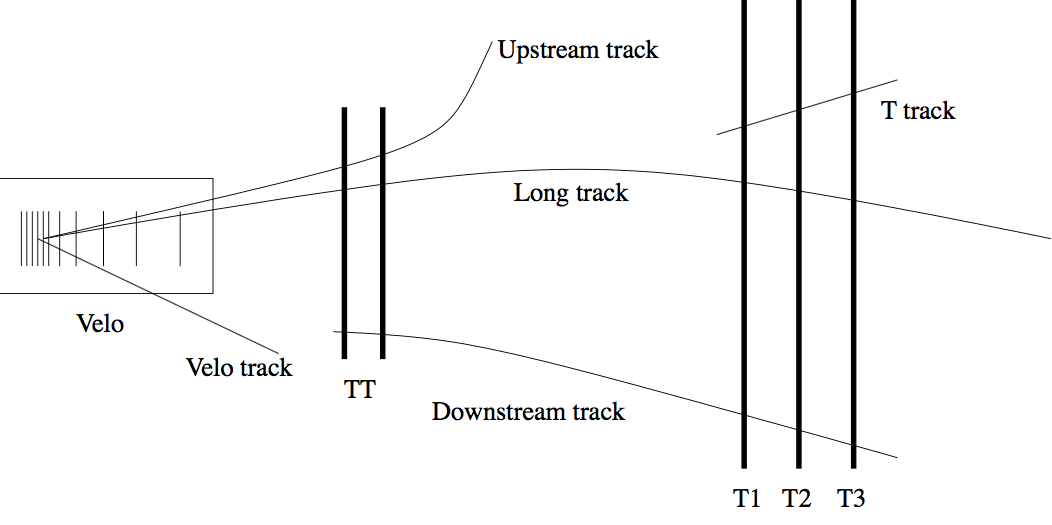
\includegraphics[width=0.8\textwidth,trim=0cm 0cm 0cm 5mm,]{Lmumu/figs/track_types.png}
\caption{Representation of possible track types in LHCb. Candidates built from ``long" and 
``downstream" tracks are used in this anlysis.}
\label{fig:track_types}
\end{figure}
 
\section{Simulation}
\label{sec:Lb_simulation}

Samples of simulated events are needed in order to train the multivariate classifier
(see Sec.~\ref{sec:Lb_mva}), calculate the selection efficiency and study possible backgrounds;
in particular for this analysis samples of $\sim 2$ millions $\Lb\to\jpsi\Lz$ and 
$\sim 5$ millions $\Lb\to\Lz\mumu$ simulated events are used.
Samples of simulated $\Bz\ra\jpsi\KS$, $\Bz\ra\KS\mumu$ and $B^{+} \ra\mumu K^{*+}$
events are also used to study backgrounds from these decays. The events are generated using
$\textsc{Pythia}8$, hadronic particle are decayed using $\textsc{EvtGen}$ and $\textsc{Geant4}$ is used to simulate
the interaction of final state particles with the detector. Simulated events are then
reconstructed using the same reconstruction software used for real data. The L0 hardware
trigger is emulated in the simulation, while for the software stage, HLT
(see Sec.~\ref{sec:det_trigger}), the same code can be used as for data.
Events are simulated using both 2011 and 2012 beam and detector conditions in the same amounts
in which data is available. While the simulation gives a generally good description of data some discrepancies remain.
However it is important that the simulation gives an accurate description of the data, 
especially for quantitative estimations, e.g the extraction of efficiencies. The next sections
describe corrections applied to the simulation in order to have a better description of data.
In Appendix~\ref{app:MC_data_comp} data distributions are compared with simulated ones for
variables relevant to this analysis.

\subsection{Decay Model}
\label{decaymodel}

Little is known about \Lb decays structure and therefore the simulation software generates events
according to the phase space given by the available kinematic. To include a reasonably realistic \qsq dependence,
the simulation is weighted using decay amplitudes based on the predictions in Ref.~\cite{Gutsche:2013pp}.
Equations in this paper are for the case of unpolarised \Lb production and for this analysis those are extended to include polarisation.
Details about the models used are in Appendix~\ref{ap:LbLmumuAngular}. The value of the \Lb production polarisation, $P_b$, 
used in the calculations is $P_b = 0.06$ as measured by LHCb~\cite{Aaij:2013oxa}. 
%In the weight calculation we always use generator level
%momenta to obtain \qsq and corresponding angles.
Figure~\ref{fig:decaymodeleffonq2} shows the phase space \qsq distribution and the one obtained re-weighting the events.
The latter can be qualitatively compared to the \qsq spectrum of a generic $\bquark\to\squark\ll$ decay
shown in Fig.~\ref{fig:q2spectrum}.
%
\begin{figure}
\centering
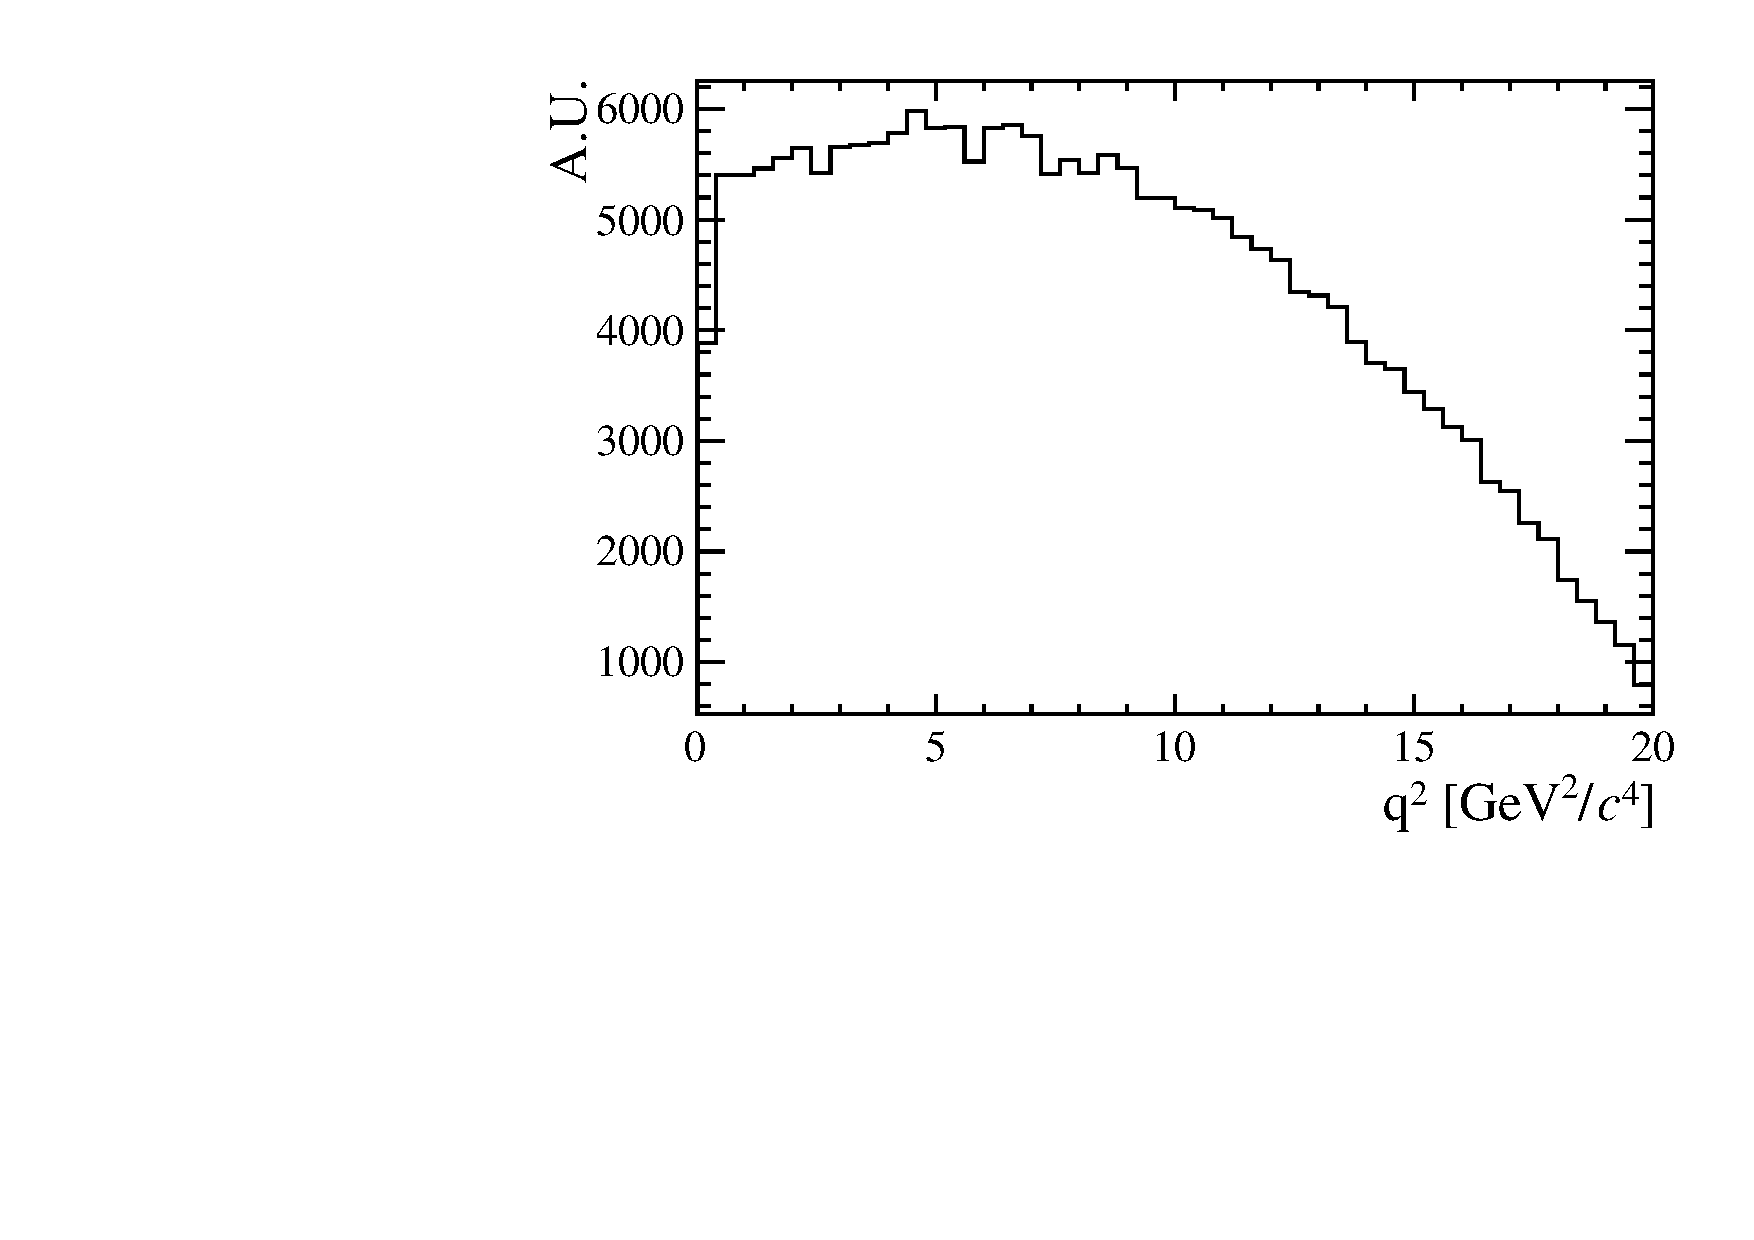
\includegraphics[width=0.48\textwidth]{Lmumu/figs/Q2_beforemodel.pdf}
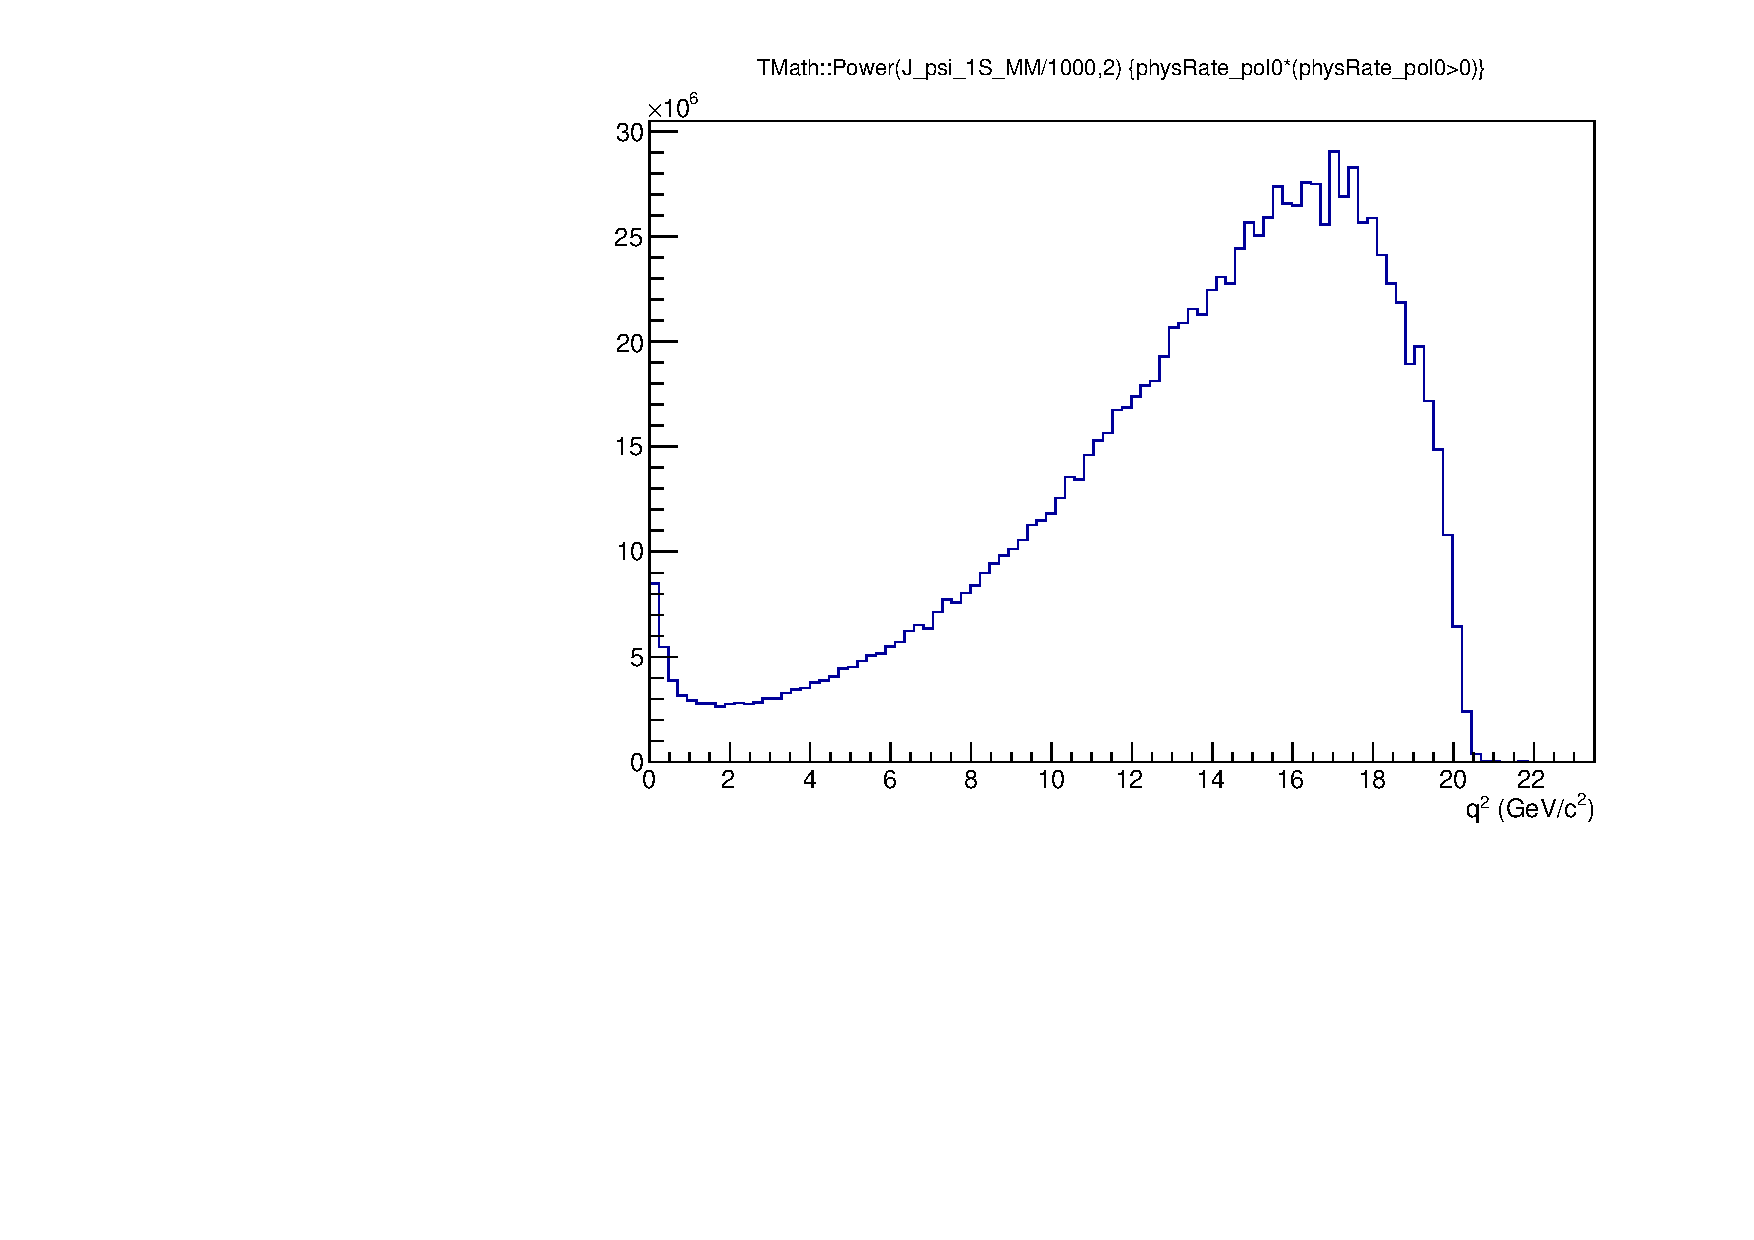
\includegraphics[width=0.48\textwidth]{Lmumu/figs/Q2_aftermodel.pdf}
\caption{The \qsq spectrum of $\Lb\to\Lz\mumu$ simulates events according to the
phase space of the decay (left) and reweighted using the decay amplitudes (right).}
\label{fig:decaymodeleffonq2}
\end{figure}
%
For the normalisation mode, the decay model used is described in Appendix~\ref{ap:LbJpsiLAngular},
with amplitude magnitudes and production polarisation taken from the measurements in
Ref.~\cite{Aaij:2013oxa}. Phases are not yet measured and are all set to zero.

\subsection{Kinematic re-weighting}
\label{sec:kinWeight}

Small data-simulation differences are found in the kinematic properties of the mother particle, \Lb,
which also affect the final state particles. The simulation is re-weighted by 
comparing the momentum and transverse momentum of \Lb between
real and simulated $\Lb\to\jpsi\Lz$ candidates which passed pre-selection (see Sec.~\ref{sec:Lb_selection}).
To do this a data sample as clean as possible is obtained selecting a narrow interval around \jpsi and \Lb peaks.
Then the \Lb invariant mass is fitted to extract the amount of background under the peak.
The background fraction, $f_b = B/(S+B)$, is then used to statistically
subtract the background from the kinematical distributions as described by the equation:
%
\begin{equation}
S(p,\pt) = T(p,\pt) - f_b\cdot B(p,\pt),
\end{equation}
\noindent
where $S(p,\pt)$ is the distribution of pure signal events, which we want to obtain, $T(p,\pt)$ is the total
distribution of signal plus background, namely the distribution of all events in the signal interval,
$5605 < m(p\pi\mumu) < 5635 \mevcc$, and $B(p,\pt)$ is the pure background
distribution obtained using events from the upper sideband, $m(p\pi\mumu) > 5800 \mevcc$.

After obtaining the signal distributions from data these are compared with \mbox{$\Lb\to\jpsi\Lz$} simulated events
and a weight, $w(p_{\Lb},\pt_{\Lb})$ is defined by taking the ratio of the two dimensional $(p,\pt)$ distributions.
The result is shown in Fig.~\ref{fig:kinWeight}, while Appendix~\ref{app:MC_data_comp} reports distributions
of sideband subtracted data in the signal and sideband regions together with weighted and unweighted simulated events.
In these plots the \Lb $p$ and \pt distributions match by construction but the re-weighting also improves the agreement 
between the kinematical distributions of all final particles. Small differences remain due to
the finite binning used for the weights calculation. Quality variables, such as the $\chi^2$ of tracks
and vertices, show little dependence on the kinematics and are relatively unaffected by the weighting procedure.

\begin{figure}
\centering
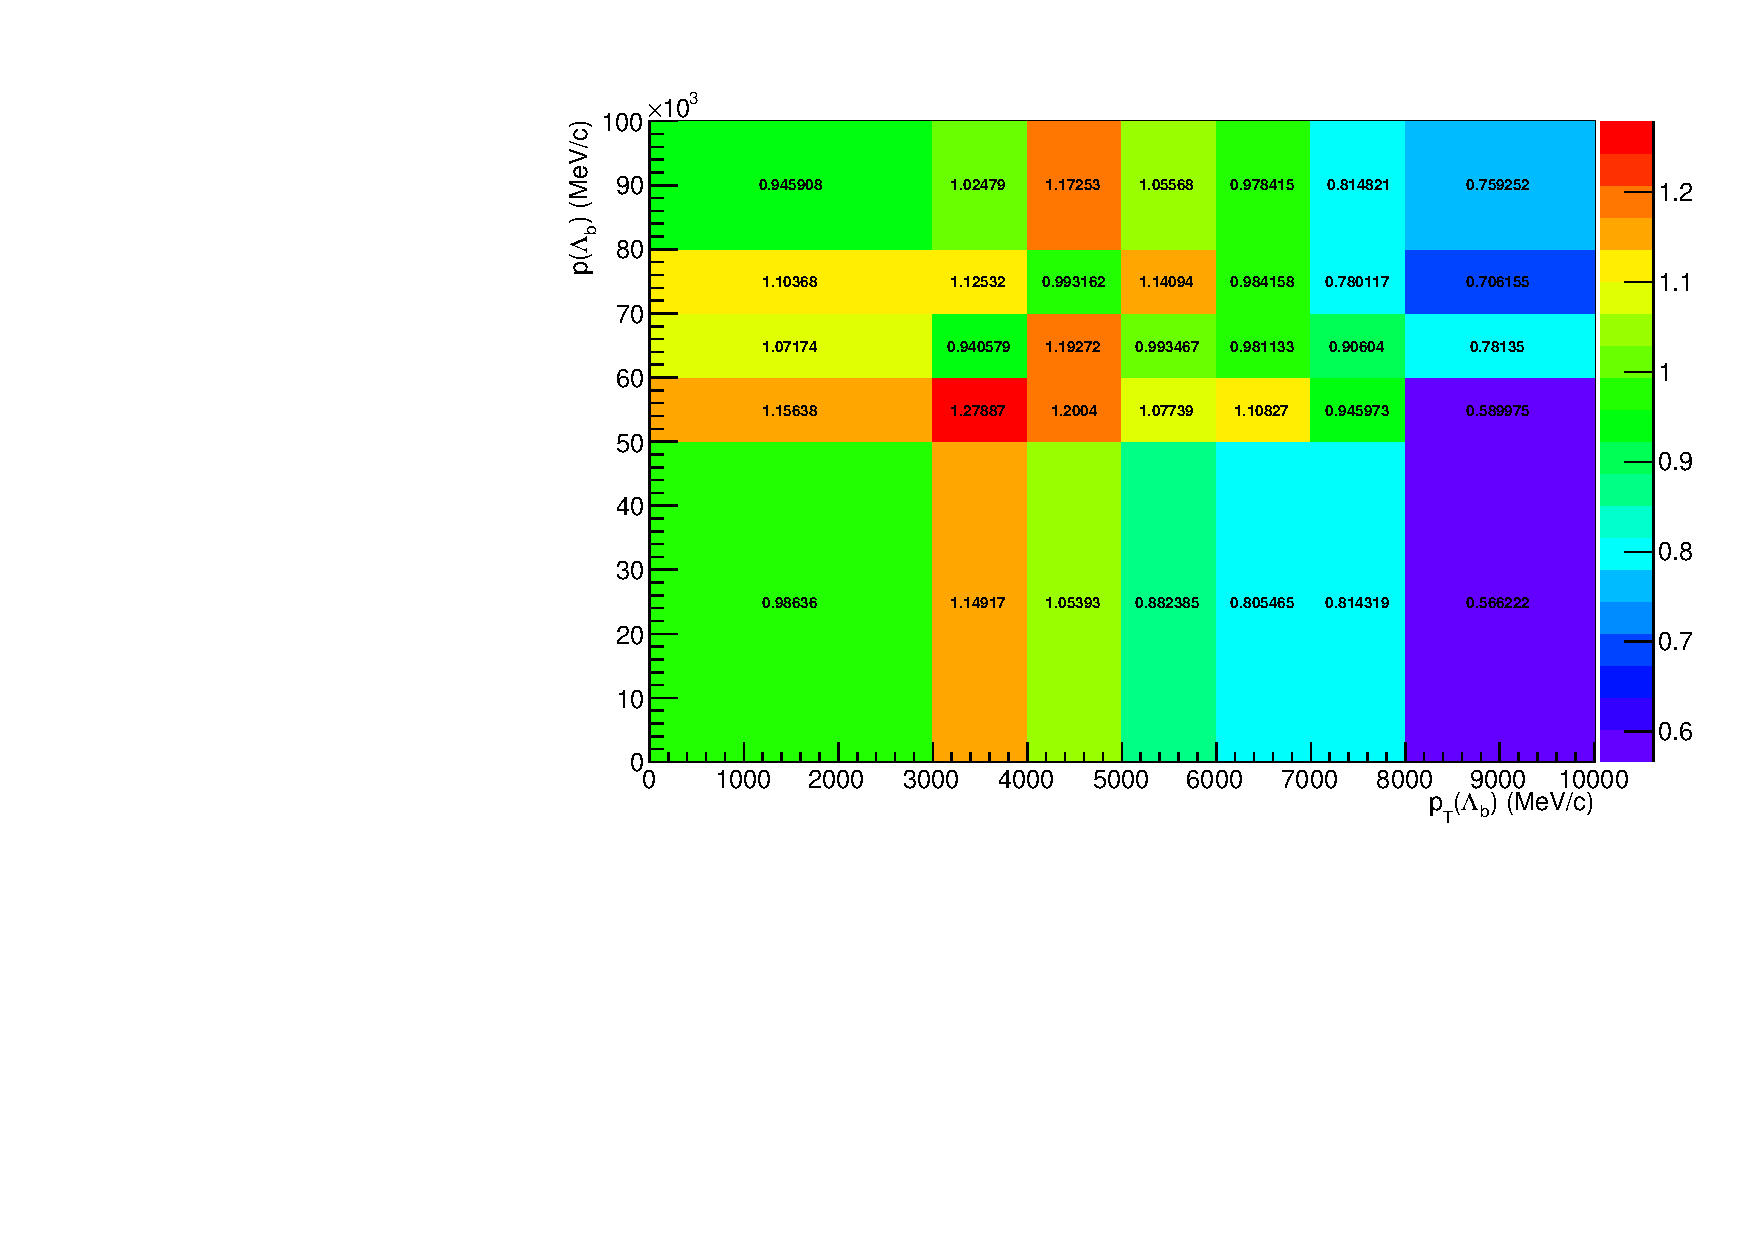
\includegraphics[width=0.9\textwidth]{Lmumu/figs/ratio_Lb_p_pt.pdf}
 \caption{Weights used for the kinematical reweighting as a function of the momentum and transverse momentum of \Lb. }
\label{fig:kinWeight}
\end{figure}

\subsection{Event type}

The fraction of \Lz baryons reconstructed from long tracks and downstream tracks does not fully agree between data and simulation.
For $\Lb\to\jpsi\Lz$ decays passing the full selection, $\sim 70\%$ of candidates are reconstructed from downstream tracks, while
they are $\sim 75\%$ in the simulation.
The fraction of downstream and long tracks also varies as a function of \qsq and the biggest differences are found at low \qsq.
In order to deal with this differences all efficiencies are obtained separately for downstream and long candidates and the analysis is done 
separately for the two categories joining results at the end. It is therefore not required to correct the simulation
to reproduce the correct fraction of events in each category.


\section{Selection}
\label{sec:Lb_selection}

This section describes the requirements applied to reconstruct $\Lb\to\Lz\mumu$ and $\Lb\to\jpsi\Lz$ candidates. 
The selection procedure is divided into two steps: a pre-selection, where cuts are applied in order to be able to work
with manageable datasets and a multivariate analysis (MVA) which combines information from several variables.
As a first step good quality tracks are selected by imposing requirements on their basic kinematic properties, 
such as the \pt of the final particles, and quality requirements, such as the track \chisq.
The selection then forms a dimuon candidate from two oppositely changed muons. 
In events containing a dimuon candidate, two oppositely charged tracks are combined
and retained as a \Lz candidate if they form a good quality vertex which is well separated
from all primary vertices. Finally, the dimuon and \Lz candidates are combined to form \Lb
baryons with requirements placed on the properties of this combination. 


\subsection{Pre-selection}
\label{sec:Lb_stripping}

The full list of pre-selection cuts is reported in Tab.~\ref{tab:Lb_stripping}.
In the table \chisqip is defined as the projected distance from a vertex
divided by its uncertainty, for example the $\chisqip(primary) > n$ requirement on $\Lb$ means
that the \Lb vertex must be at least $\sqrt{n}$ standard deviations away from the primary vertex.
Another quantity, found to be particularly powerful at removing combinatorial background, is a pointing 
variable called DIRA defined as the cosine of the angle between the direction of a particle's momentum 
and the flight direction from its mother vertex. Requiring a DIRA close to unity corresponds to 
the selection of particles with well-defined origin vertices.
Figure~\ref{fig:IPandDIRA} shows graphical representations of the \chisqip and DIRA variables.
%
\begin{figure}[hb]
\centering
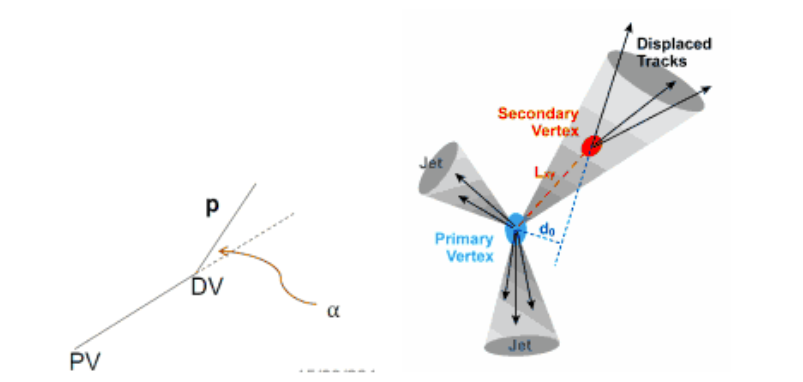
\includegraphics[width=0.8\textwidth]{Lmumu/figs/IPandDIRA.png}
\caption{Graphical representation of the DIRA (left) and \chisqip (right) variables.}
\label{fig:IPandDIRA}
\end{figure}
%
The variable $\chisq_{\rm FD}$ represents the flight distance of a particle from its origin vertex
divided by the corresponding uncertainty. The $\chisq_{trk}$/ndf and $\chisq_{vtx}$/ndf quantities 
are the $\chisq$ from the fit to tracks and vertices, which are used to quantify their quality.
The \verb!GhostProb! quantity describes the probability of a track being fake.
By construction, cutting at a value of $k$, removes $(1 - k)\cdot 100 \%$ of fake tracks.
The \verb!hasRich!, \verb!hasCalo! and \verb!isMuon! variables are binary indicators that
the information from the RICH, calorimeter and muon detectors is available for the track.
Loose PID requirements on the proton are also applied in the pre-selection.
Details about PID quality estimators are given in Sec.~\ref{sec:PID_perf}.
%To quantify the probability of particular particle identity a combined likelihood is calculated
%combining information from the calorimeters, the RICH and the Muon detectors.
%The pion hypothesis is used as a reference point and the probability of a specific ID is given
%in terms of the difference between the Log-Likelihood of the given hypothesis and the pion.
%This variable is called is called Delta Log-Likelihood (DLL) and denoted with \verb!PID!.
%For example:
%\begin{equation}
%\verb!PID!_K = \text{DLL}_{K-\pi} = \log(\mathcal{L}_K) - \log(\mathcal{L}_\pi)
%\end{equation}
%quantifies the probability of a particle being a kaon rather than a pion.
%For details about the definition of the variables used see Ref. \cite{Loki_twiki}.
A large mass window around the \Lb peak is used to allow a fit to the sideband to be performed 
and to use sideband candidates to train a multivariate classifier.
Rare candidates are selected by the \qsq region requirements described in Sec.~\ref{sec:Lb_q2choice},
while resonant candidates are further constrained to have dimuon invariant masses
in a 100~\mevcc~interval around the known \jpsi mass~\cite{PDG2014}.

\begin{table}[h]
\centering
      \begin{tabular}{$l^c}
      \rowstyle{\bfseries}
Particle     			&  	Requirement          \\ \hline
\multirow{5}{*}{\Lb}            	&  	$4.6 < m(p\pi\mu\mu) < 7.0$ \gevcc \\
            				& 	$\texttt{DIRA}>0.9999$          \\
					& 	$\chisqip<16.0$               \\
            				& 	$\chisq_{\rm FD}>121.0$             \\
            				& 	$\chisq_{vtx}/\text{ndf}<8.0$          \\ \hline
\multirow{3}{*}{\Lz}      	& 	$\chisq_{vtx}/\text{ndf}<30.0(25.0)$              \\
         				& 	Decay time $>2$ ps              \\
					& 	$|m(p\pi)-m^{\rm PDG}_\Lz|< 35(64)$~\gevc        \\ \hline
\multirow{3}{*}{$p$/$\pi$}	& 	$p>2$ \gevc           \\ 
					& 	$\pt>250$ \mevc           \\  
            				& 	$\chisqip>9(4)$              \\ \hline
\multirow{2}{*}{$p$ (only long cand.) } 	&   	\verb!hasRICH!    \\
					&   	$\verb!PID!p>-5$  \\  \hline
\multirow{5}{*}{$\mu$}       &   	\verb!isMuon!    \\
					& 	$\chisq_{trk}/\text{ndf}< 5$ 		\\
					& 	$\verb!GhostProb!<0.4$	\\
            				& 	$\verb!PID!\mu>-3$		\\
            				& 	$\chisqip>9.0$        \\      \hline
\multirow{2}{*}{Dimuon}     & 	$\chisq_{vtx}//\text{ndf}<12.0$          \\
            				&	$|m(\mu\mu) - m^{\rm PDG}_\jpsi|< 100$~\mevcc ~~($\jpsi\Lz$ only)       \\ \hline
      \end{tabular}
\caption{Summary of the pre-selection requirements. Where two values are given,
the main one applies to long candidates and the one in parenthesis to downstream candidates.}
\label{tab:Lb_stripping}
\end{table}


\subsection{Neural Networks}
\label{sec:Lb_mva}

The final selection is performed using a neural network classifier based on the NeuroBayes package.
%~\cite{Feindt:2006pm,feindt-2004}
 The input to the neural network consists of 14 variables carrying 
information about the kinematics of the decay, the quality of tracks and vertices and the PID of the muons.
The list of the 10 most significant inputs is reported in Tab.~\ref{tab:Lb_nnInputs}, together with information 
about the importance of each input.
%
%In appendix \ref{app:MC_data_comp} we report comparisons between the variable used in data and Monte Carlo.
%On data we extract the signal distribution using the sideband subtraction technique.
%
%Under ``adds" is shown how much discriminating power a variable adds with respect to the previous ones.
%Under ``only this" is shown how much power each single input has independently of all others. Under ``loss" 
%is provided information about how much power is lost if each single input is removed.
%
Variables related to \Lz and its daughters are considered as different inputs depending on the
candidate type (long or downstream). This effectively corresponds to making a separate
training for the two categories. 
%Further details on the definition and calculation of the
%variables importance is available in Ref.~\cite{LHCb-ANA-2011-094}.
%The graphical representation of the correlation matrix is shown in Fig.~\ref{fig:Lb_nnCorrelation},
%where the variable with ID$ = 1$ is the neural network output and the IDs of the other variables are 
%listed in Tab.~\ref{tab:Lb_nnInputs}.

The neural network is trained using representative samples of signal and background.  A sample of simulated 
$\Lb\to\Lz\mumu$ candidates is used as a proxy for the signal, while for the background a representative sample
is given by candidates in the upper $m(p\pi\mu\mu)$ invariant mass sideband. Only the upper sideband,
$m(p\pi\mu\mu) > 6 \gevcc$, is used since it contains only combinatorial background,
while the lower sideband may contain partially-reconstructed and misreconstructed candidates.
In the \qsq spectrum of background samples the \jpsi and \psitwos peaks are still present indicating that charmonium
resonances are often combined with other random tracks. These candidates do not give a good description of purely
combinatorial background and, in order to avoid biases, they are removed from the training
sample by rejecting candidates in a 100~\mevcc~interval around the nominal \jpsi and \psitwos masses~\cite{PDG2014}.
%The events above $6 \gevcc$ used for training are not used in the subsequent analysis. 
%For the signal the training is performed combining simulated $\Lb\to\Lz\mumu$ events corresponding 
%to the beam conditions in both years. %Only triggered events are used for training.
A total of $3\cdot10^4$ events is used for the training from each sample. This corresponds to approximately
$\simeq 50\%$ of the available sideband data and $\simeq 20\%$ of the simulated sample. The full simulated sample 
is not used in the training as the same sample will also be used to study efficiencies. For reproducibility 
the events are sampled uniformly.

The single most important variable used for downstream candidates is the transverse momentum of
\Lz, which allows random combinations of tracks to be rejected as these have preferentially low \pt.
In contrast, for long candidates the most powerful variable is $\chisq_{\rm DTF}$, the \chisq from a kinematic 
fit (see Sec.~\ref{sec:DTF}) that constrains the decay products of the \Lb, the \Lz and the dimuon, to originate from their respective vertices. 
%performed using the \verb!DecayTreeFitter! tool .
Other variables that contribute significantly are the \chisqip of \Lb, \Lz and muons,
the separation between the \Lb and \Lz vertices and, finally, the muon PID.

Figure~\ref{fig:Lb_nnDist} shows distributions of neural network output for the signal and background samples
and purity, $P=N_{\mathrm{sig}}/N_{\mathrm{bkg}}$, as a function of the neural network output.
To check for potential overtraining, the distributions from test samples are also overlaid. These are found to 
follow the same shape but with different fluctuations
giving no significant evidence of overtraining. In general it can be concluded that the neural network
is able to separate signal from background and the training converged properly.
%
\begin{table}
\centering
\caption{Summary of the 10 most significant inputs to the neural network in order of importance.
%Column ``ID'' lists the indices used for the correlation matrix in Fig.~\ref{fig:Lb_nnCorrelation}.
Column ``adds'' gives the significance added by a given input when it is added to the list of those
ranked above. Column ``only this'' provides the power of a given input alone and ``loss'' shows 
how much information is lost when removing only a given input.}
\begin{tabular}{$l^c^c^c}
\rowstyle{\bfseries}
Input                     			& adds 		& only this & loss \\ \hline
\Lz$_{\rm DD}$ \pt                  		& 143.11 		& 143.11 	& 29.20  \\
$\chi^2_{\rm DTF}$       		& 77.81 		& 134.00 	& 51.10  \\
min(\chisqip $\mu$)             	& 61.31 		& 113.62 	& 29.76  \\
\chisqip \Lb                    		& 52.94 		& 113.23 	& 40.98  \\
\chisqip $\pi_{\rm LL}$              	& 20.29 		& 60.72 	& 12.82  \\
min(PID $\mu$)                   	& 17.91 		& 59.11 	& 13.44  \\
$\tau_{\Lb}$       		        	& 16.24 		& 35.36 	& 11.24  \\
\Lb \verb!DIRA!                         	& 12.28 		& 73.96 	& 9.98 	 \\
\Lz$_{\rm DD}$ flight distance       	& 9.47 	  	& 86.75 	& 11.24  \\
\chisqip \Lz$_{\rm DD}$              	& 10.58 		& 59.84 	& 8.88 	 \\
%Input                     			& ID  & adds 		& only this & loss \\ \hline
%\Lz$_{DD}$ \pt                  		& 15 	& 143.11 		& 143.11 	& 29.20  \\
%$\chi^2_{\rm DTF}$       		& 2 	& 77.81 		& 134.00 	& 51.10  \\
%min(\chisqip $\mu$)             	& 7 	& 61.31 		& 113.62 	& 29.76  \\
%\chisqip \Lb                    		& 5 	& 52.94 		& 113.23 	& 40.98  \\
%\chisqip $\pi_{LL}$             	& 16 	& 20.29 		& 60.72 	& 12.82  \\
%min(PID $\mu$)                  	& 8 	& 17.91 		& 59.11 	& 13.44  \\
%$\tau_{\Lb}$       		        & 3 	& 16.24 		& 35.36 	& 11.24  \\
%\Lb DIRA                        		& 4 	& 12.28 		& 73.96 	& 9.98 	 \\
%\Lz$_{DD}$ flight distance      	& 14 	& 9.47 	  	& 86.75 	& 11.24  \\
%\chisqip \Lz$_{DD}$             	& 13 	& 10.58 		& 59.84 	& 8.88 	 \\
%max(\chisqip $\mu$)             	& 6 	& 9.51  		& 97.24 	& 8.15 	 \\
%\chisqip \Lz${}_{LL}$           	& 10 	& 7.31 		& 54.27 	& 10.32  \\
%max(PID $\mu$)                  	& 9 	& 6.99 		& 69.33 	& 6.87 	 \\
%$\pi_{LL}$ \pt                  		& 18 	& 6.13 		& 47.03 	& 7.12 	 \\
%\Lz${}_{LL}$ \pt         	    		& 12 	& 5.58 		& 49.64 	& 5.86 	 \\
%\chisqip $p_{LL}$               	& 17 	& 4.48 		& 53.01 	& 4.18 	 \\
%\chisqip $p_{DD}$               	& 20 	& 3.43 		& 55.09 	& 3.31 	 \\
%\Lz$_{LL}$ flight distance     	& 11 	& 0.87 		& 52.52 	& 0.86 	 \\
%$p_{DD}$ \pt                    		& 21 	& 0.74 		& 129.58 	& 0.75 	 \\
%\chisqip $\pi_{DD}$             	& 19 	& 0.24 		& 70.43 	& 0.24 	 \\
\hline
\end{tabular}
\label{tab:Lb_nnInputs}
\end{table}
%
%\begin{figure}
%\centering
%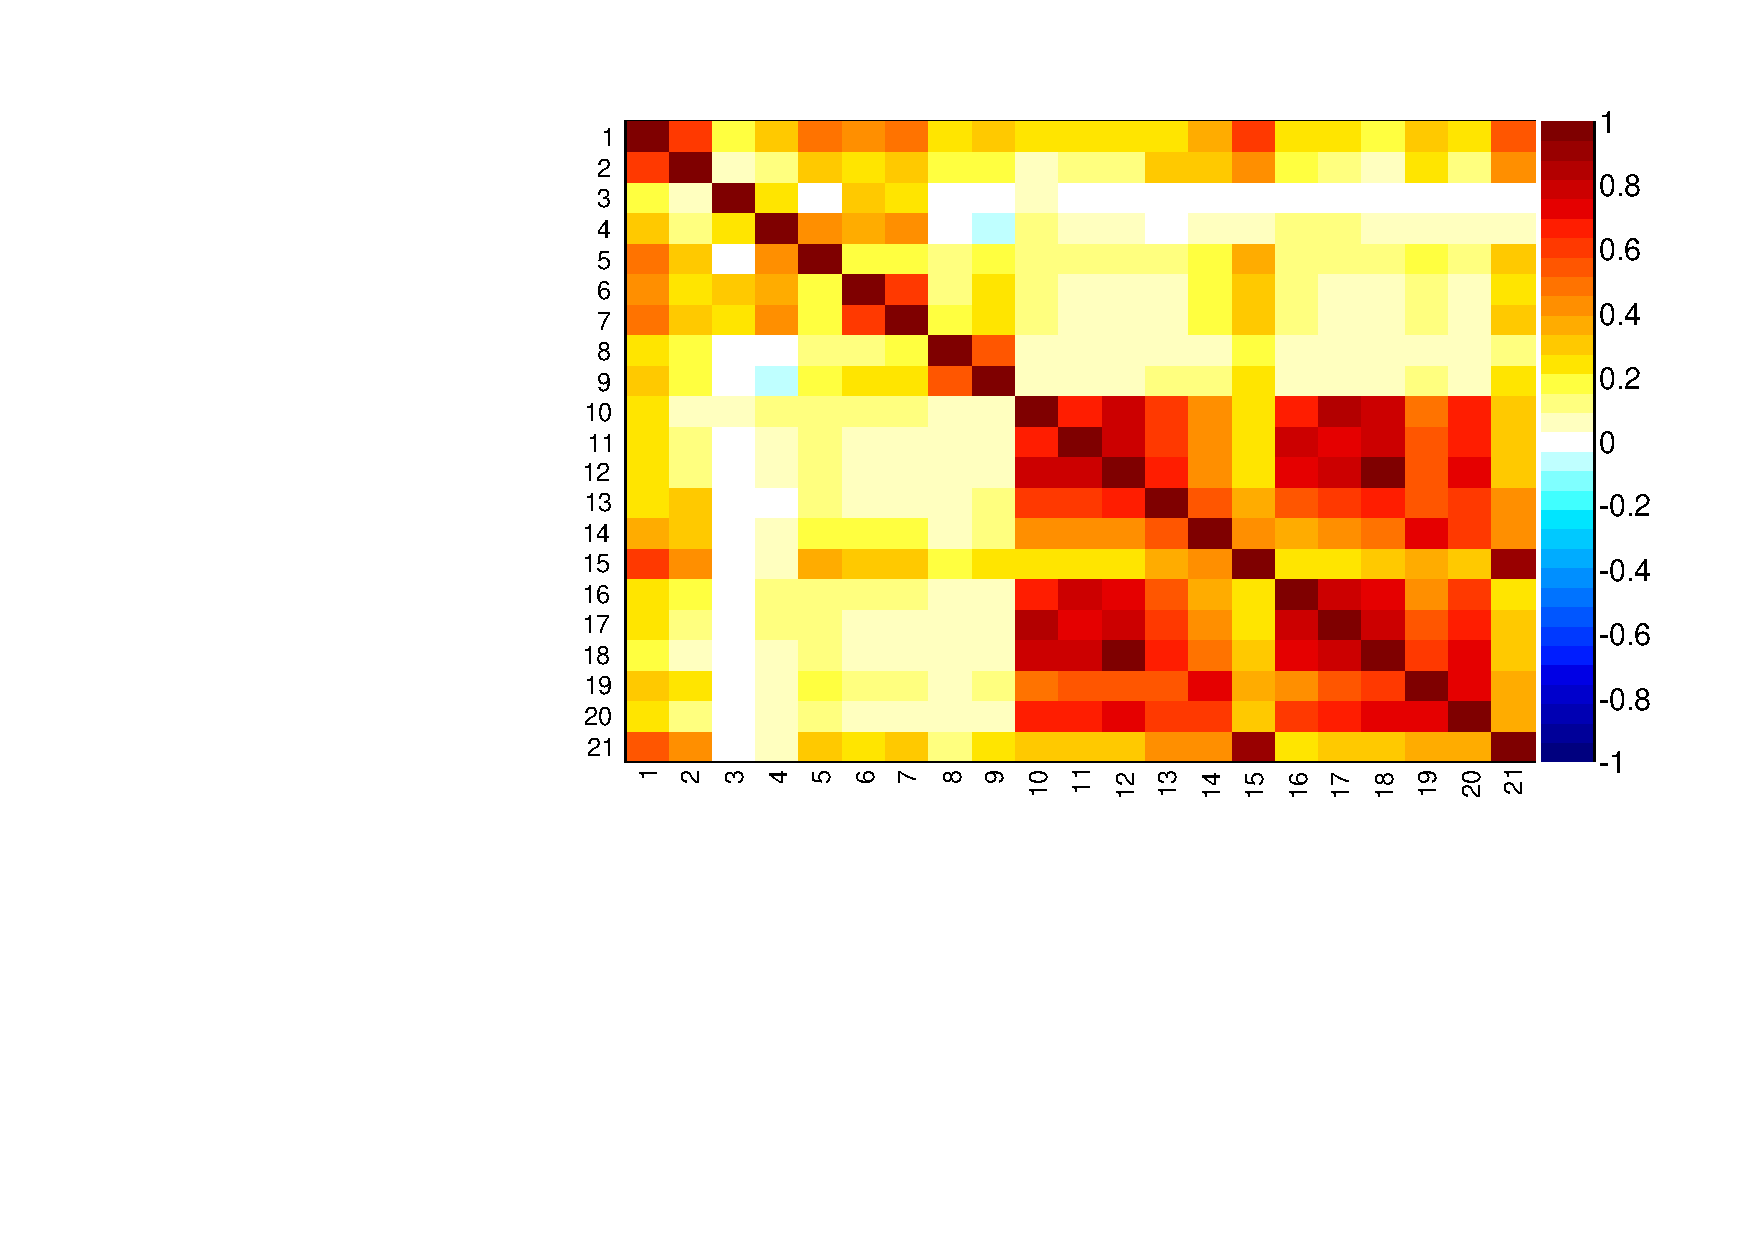
\includegraphics[width=0.7\textwidth]{Lmumu/figs/correlation.pdf}
%\caption{Graphical representation of the correlation matrix between neural network inputs.
%Column/row number 1 is the correlation to the neural network output. All
%others give the correlation between inputs with numbering scheme corresponding
%to the ID column of Tab.~\ref{tab:Lb_nnInputs}. 
%Correlation is calculated using all events without distinguishing signal and background.
%}
%\label{fig:Lb_nnCorrelation}
%\end{figure}
%
\begin{figure}
\centering
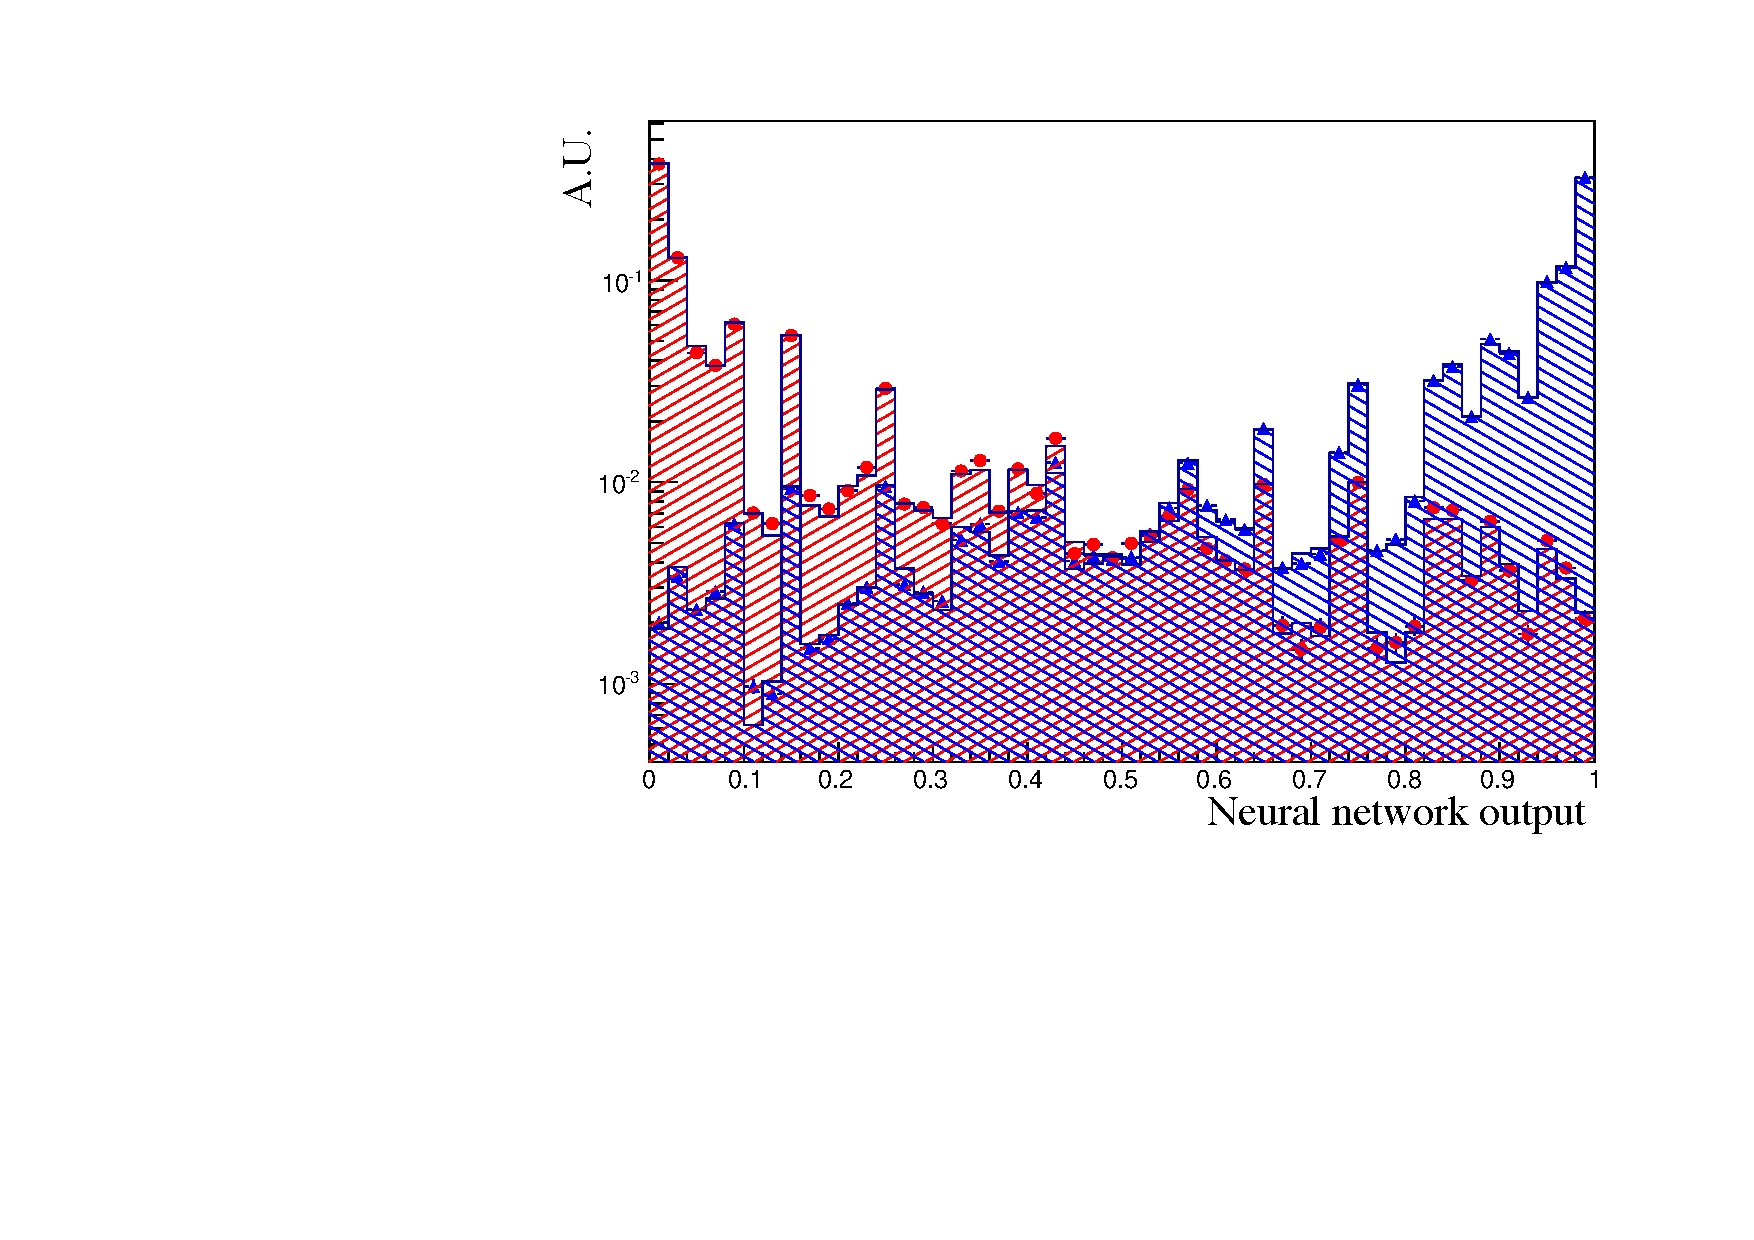
\includegraphics[width=0.49\textwidth]{Lmumu/figs/TrainAndTest.pdf}
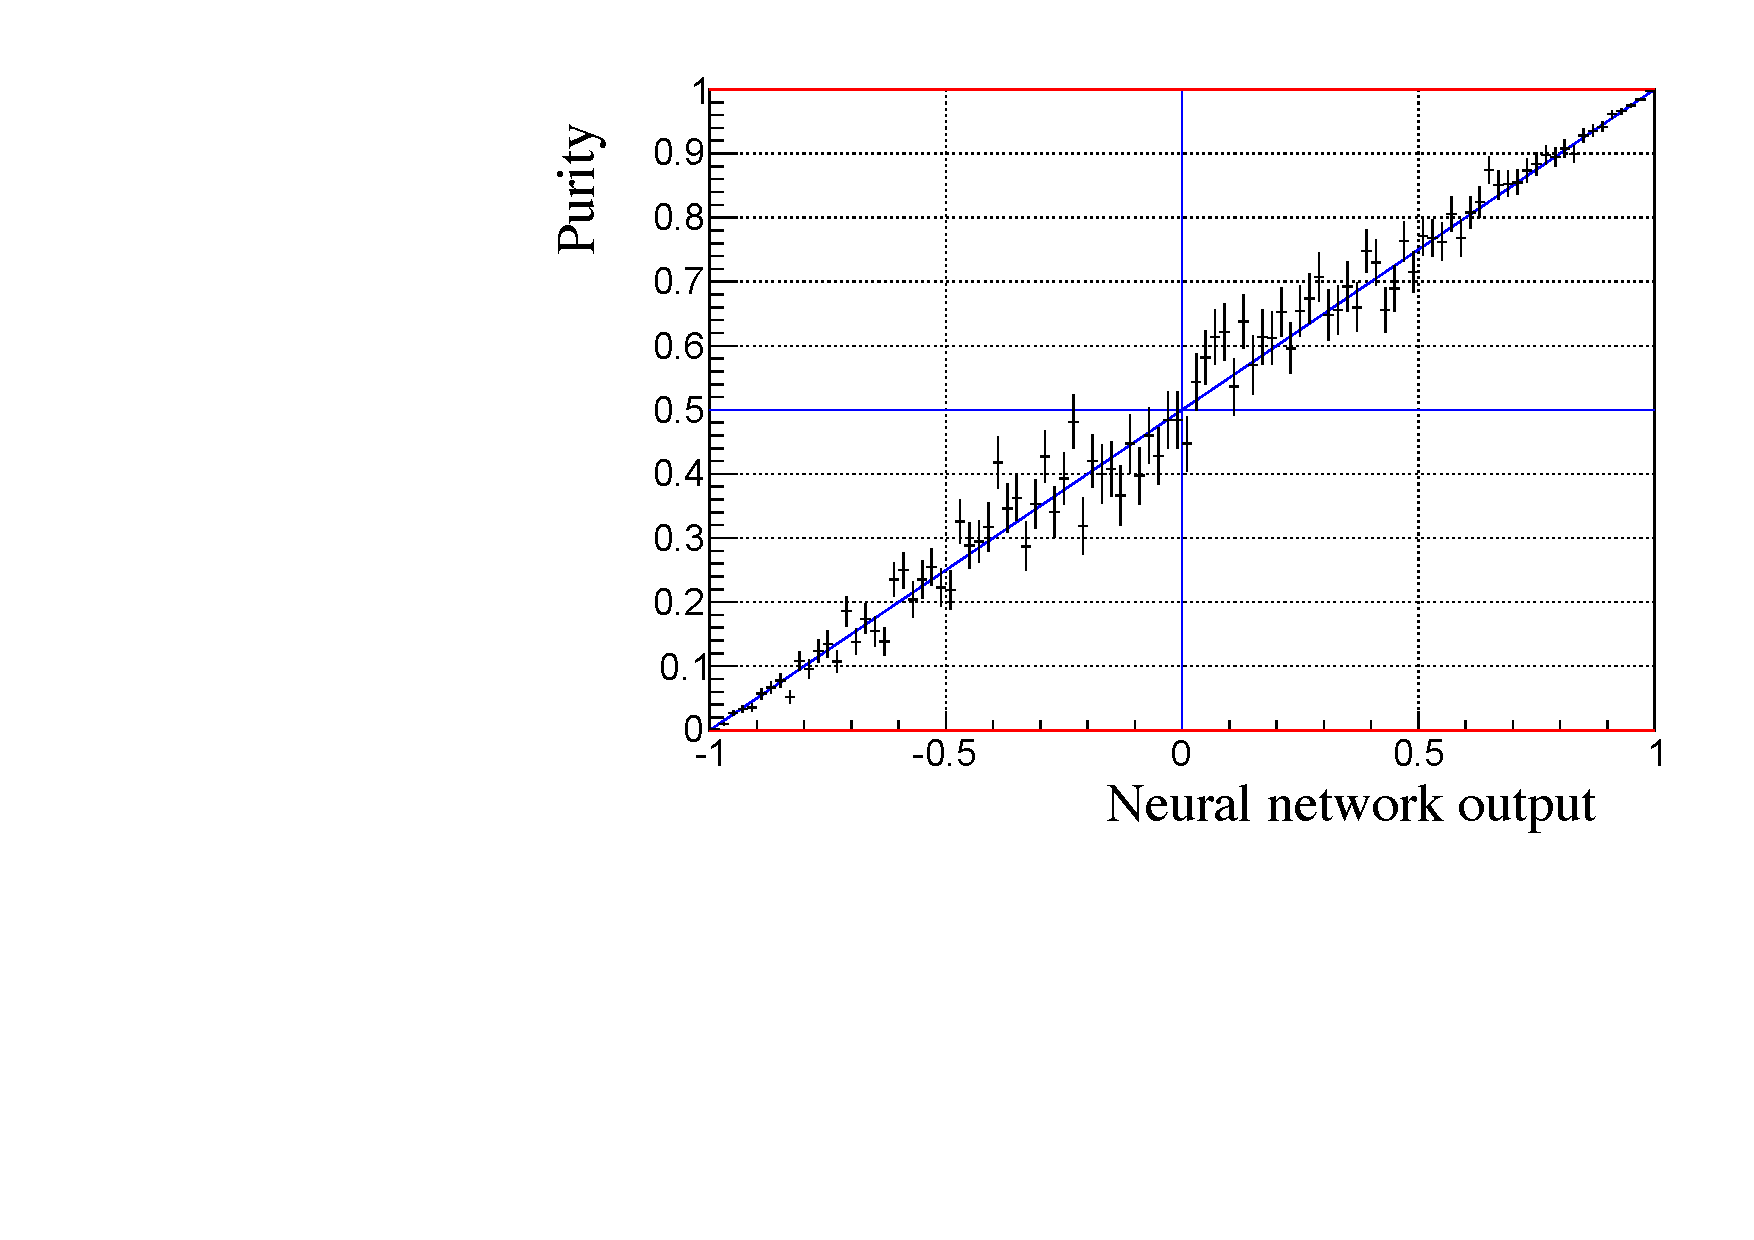
\includegraphics[width=0.49\textwidth]{Lmumu/figs/purity_NN.pdf}
\caption{(left) Neural network output distribution for training (points) and test (stripes) samples,
for signal (blue) and background (red) candidates. (right) Purity as a function of neural network output.}
\label{fig:Lb_nnDist}
\end{figure}

If too much information is given as inputs, the classifier can become able to infer
 the 4-body invariant mass of the candidates from its inputs.
This can generate fake peaks and it is therefore important to check
for correlations between the 4-body invariant mass and the neural network output.
Figure~\ref{fig:Lb_NNprofiles} reports the average neural network output as a function of
the 4-body $m(p\pi\mu\mu)$ invariant mass for data and simulation. The distributions
are flat indicating that no significant correlation is present.
%
\begin{figure}
\centering
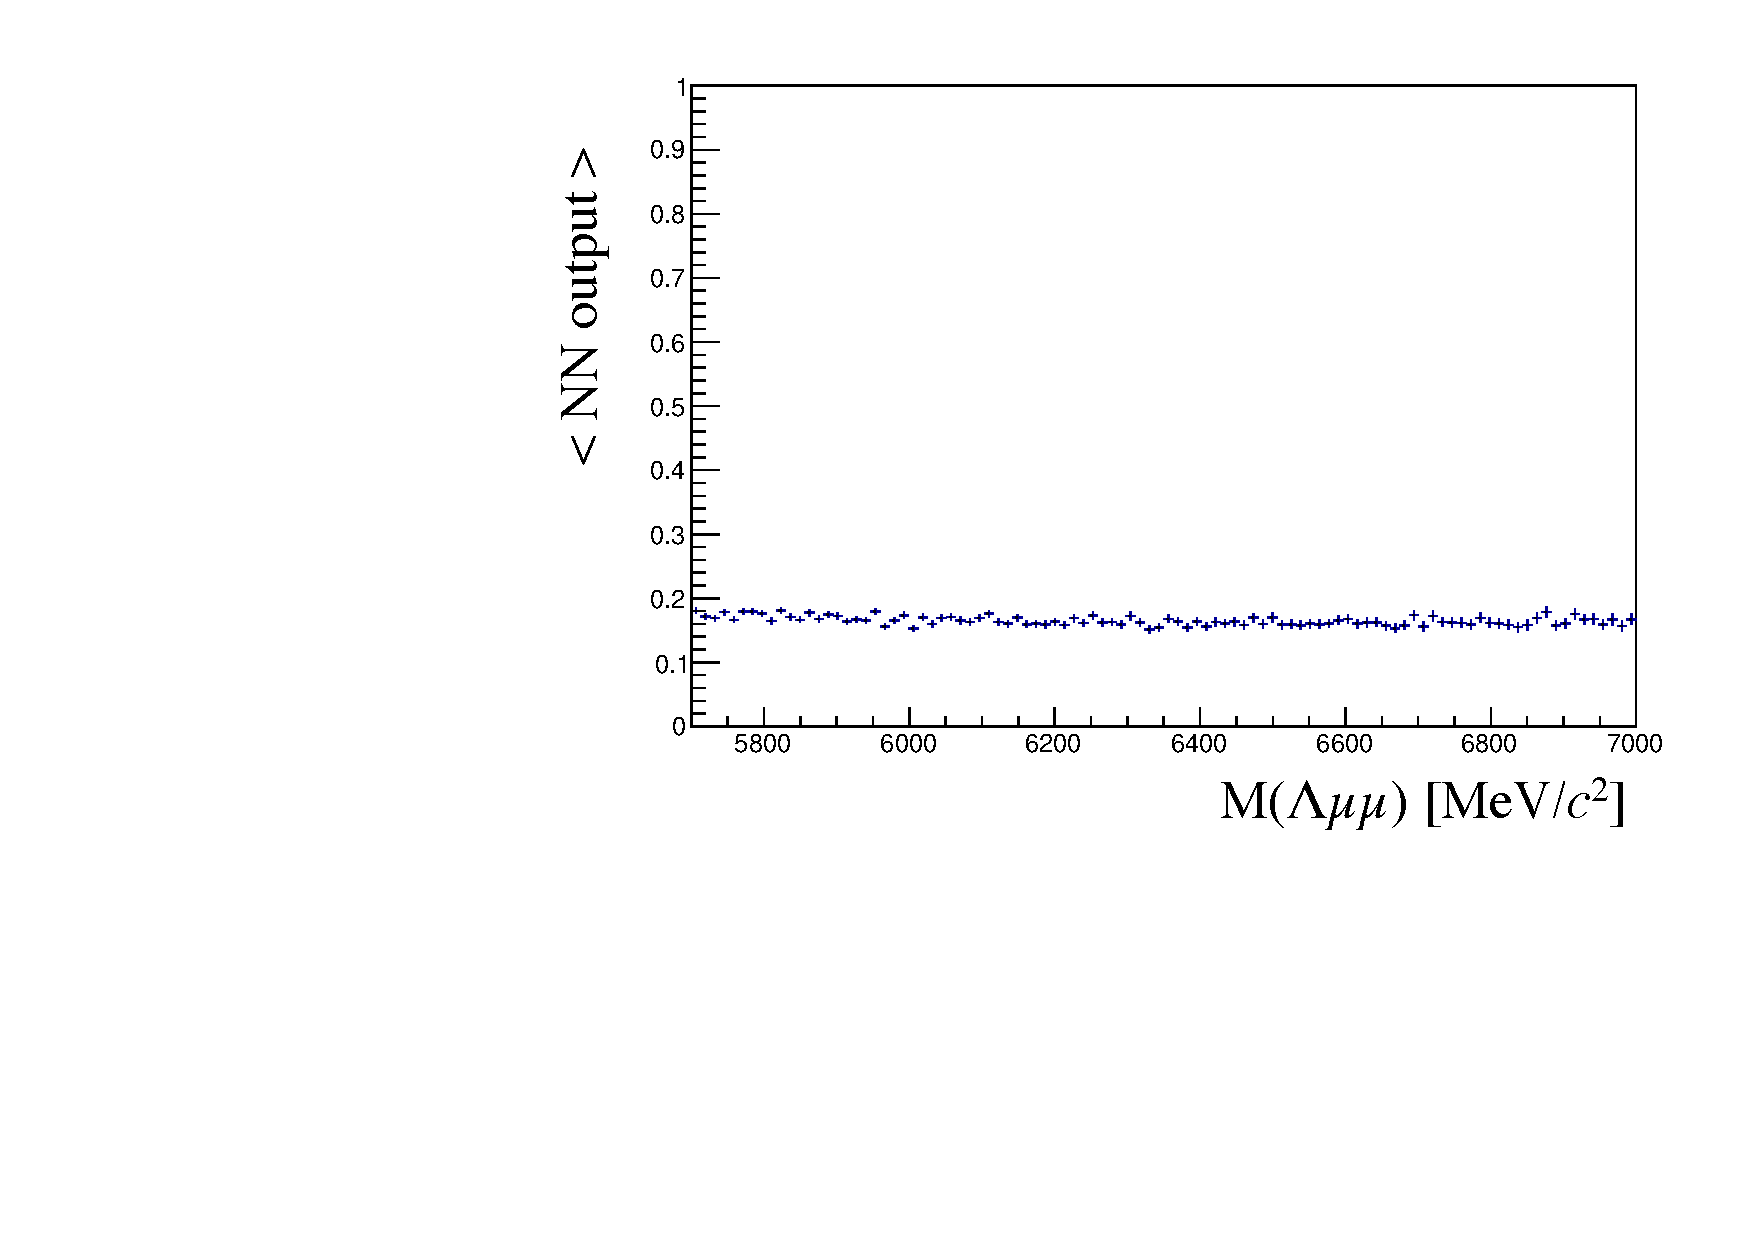
\includegraphics[width=0.49\textwidth]{Lmumu/figs/NNout_profile_vs_LbMM_bkgData.pdf}
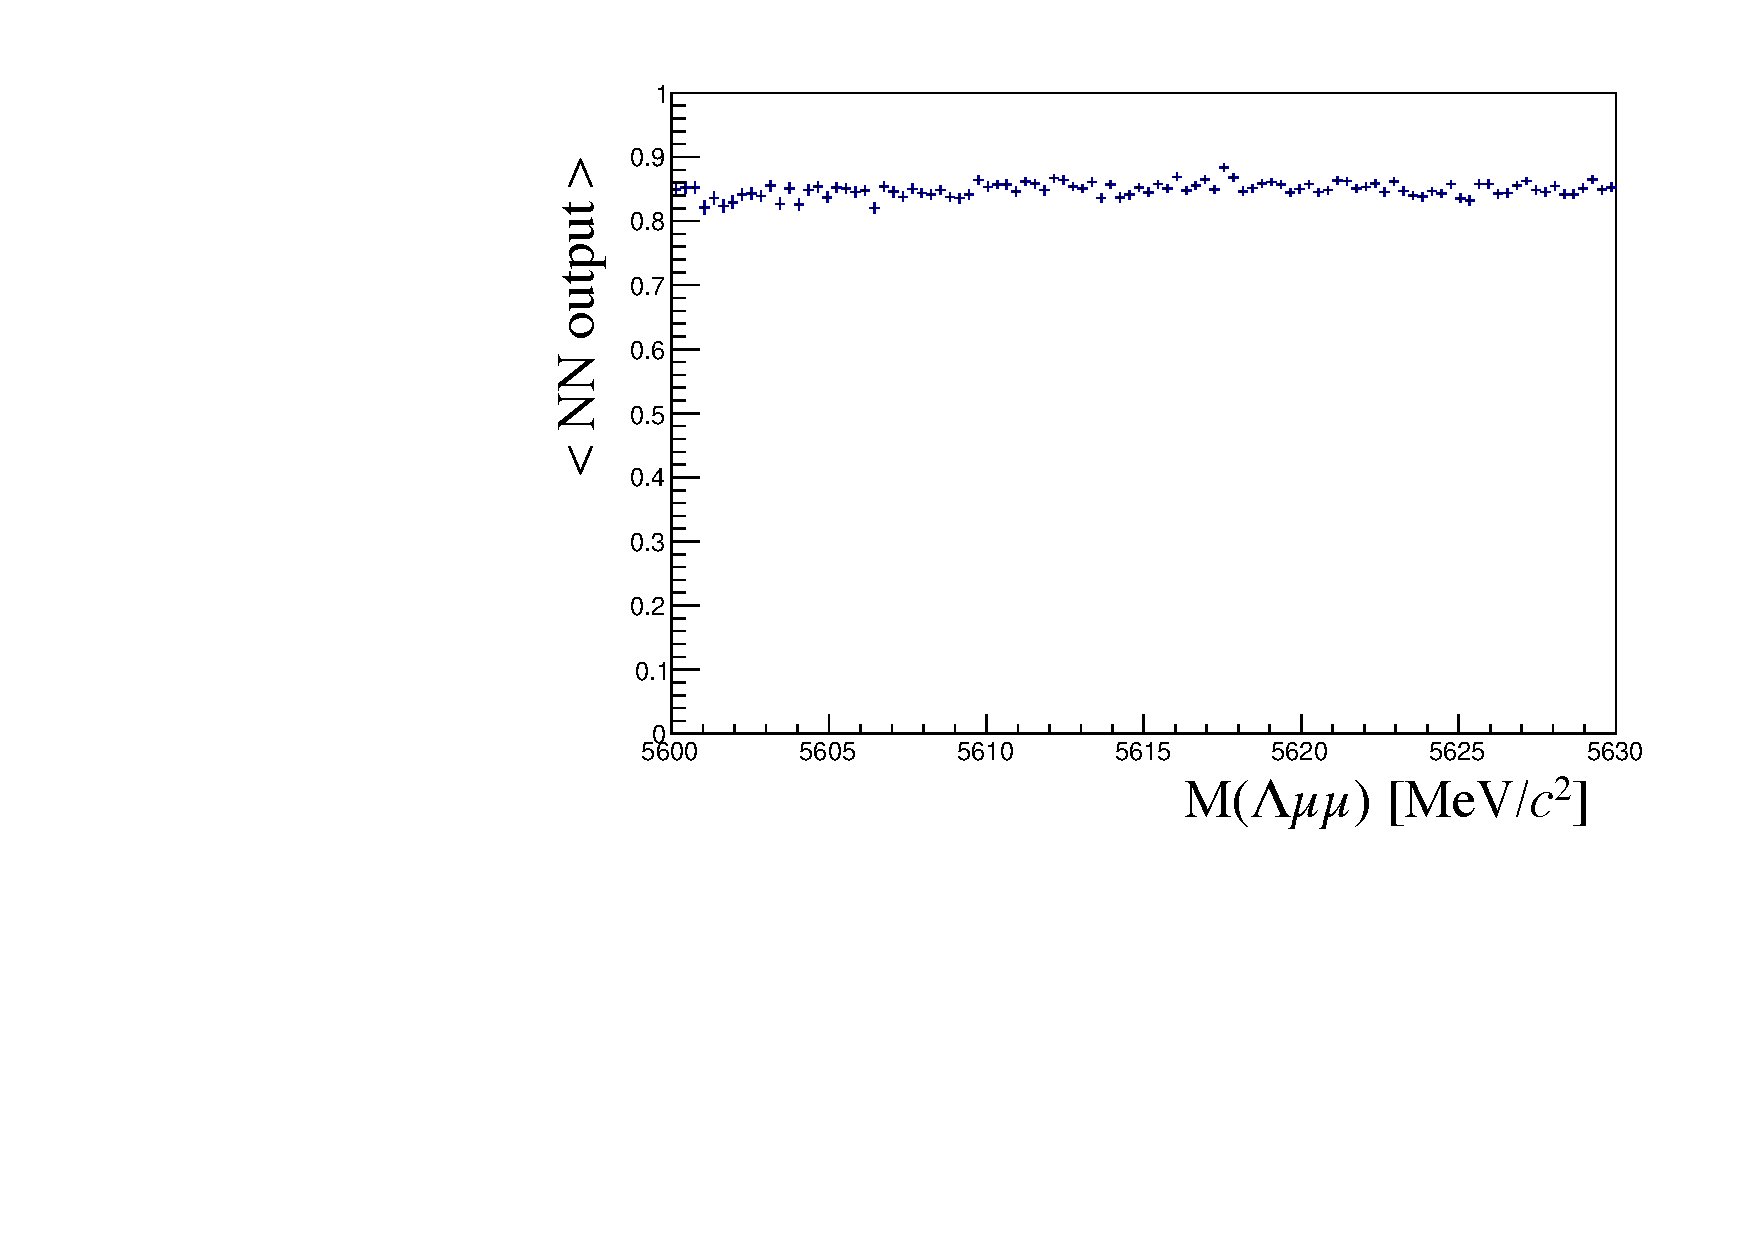
\includegraphics[width=0.49\textwidth]{Lmumu/figs/NNout_profile_vs_LbMM_MCsignal.pdf}
\caption{Average value of neural network output as a function of the 4-body invariant mass 
for data sideband (left) and simulated signal (right) candidates.}
\label{fig:Lb_NNprofiles}
\end{figure}




%As side note, we do not imply any particle identification on the \Lz daughters, nor we explicitly
%veto contributions where \KS is misreconstructed as \Lz. As will be seen later, \Bz decays
%containing \KS do not pose significant issues and any sensible attempt to significantly suppress
%them would result in significant loss of the statistics.




\subsection{MVA optimisation}
\label{sec:Lb_mva_opt}

In the high-\qsq region, where the signal is already observed, the requirement on the neural network output
is chosen to maximise the significance, $N_{\mathrm{S}}/\sqrt{N_{\mathrm{S}}+N_{\mathrm{B}}}$, where
$N_\mathrm{S}$ and $N_\mathrm{B}$ are the numbers of expected signal and background candidates respectively.
$N_\mathrm{S}$ is derived from simulation but, as an arbitrary number of events can be generated, it
needs to be normalised. To do this, the invariant mass distribution of real $\Lb\to\jpsi\Lz$ candidates
is fit after pre-selection (including all requirements except the MVA selection). This is possible as the peak of the resonant
channel is already clearly visible before the MVA requirement. The resonant yield is then scaled by the ratio
of the $\Lb\to\Lz\mumu$ and $\Lb\to\jpsi\Lz$ branching fractions as measured 
by LHCb using 2011 data~\cite{LHCb-PAPER-2013-025}, 
\begin{equation}
\BR(\Lb\to\Lz\mumu) / \BR(\Lb\to\jpsi\Lz) =  1.54 \times 10^{-3},
\end{equation}
\noindent
and by the $\jpsi\to\mumu$ branching fraction, \emph{i.e.}
\begin{equation}
N_\mathrm{S} = N_\jpsi \cdot \frac{\BR(\Lb\to\Lz\mumu)}{\BR(\Lb\to\jpsi\Lz) \cdot \BR(\jpsi\to\mumu) }.
\end{equation}
%
The number of expected background candidates is derived by fitting the data
sideband with an exponential function and extrapolating into the signal region.

In the low-\qsq region, where the signal is unobserved, the so called ``Punzi figure-of-merit",
$N_{\mathrm{S}}/(n_\sigma/2+\sqrt{N_{\mathrm{B}}})$, is maximised~\cite{Punzi:2003bu}.
This figure-of-merit is considered to be optimal for discovery and the parameter $n_\sigma$ corresponds to
the number of expected standard deviations of significance, in this analysis $n_\sigma = 3$ is used.
Moreover, the Punzi shape does not depend on the relative normalisation between signal and background, which
is important since the signal is still unobserved at low-\qsq and the existing predictions vary significantly
for this region. The dependence of the figure-of-merit for both \qsq regions is shown in Fig.~\ref{fig:Lb_FOM}, and curves
of signal efficiency versus background rejection are shown in Fig.~\ref{fig:Lb_ROC}.

For the final selection the neural network output is required to be larger than 0.76 for candidates in the high-\qsq region
and 0.97 for the low-\qsq ones. Using these requirements the neural network retains approximately 97\% (82\%) of long 
candidates and 96\% (66\%) of downstream candidates for the high- (low-) \qsq selection, with respect to
the pre-selected samples. After the full selection has been applied $\sim 0.5$\% of the events contain multiple candidates.
In these cases candidates are rejected randomly such that only one is retained per event. 
%which are randomly rejected keeping only one candidate per event. 
%
%As reminder, in low-\qsq region we start with much larger background than in high-\qsq region.
%Moreover, while background rejection looks similar at selected requirement, in terms of amount of background kept, there is huge difference. 
%
To normalise the branching ratio measurement, $\Lb\to\jpsi\Lz$ candidates are selected using both, low- and high-\qsq, 
MVA requirements to normalise respectively low and high-\qsq intervals. 
%
\begin{figure}
\centering
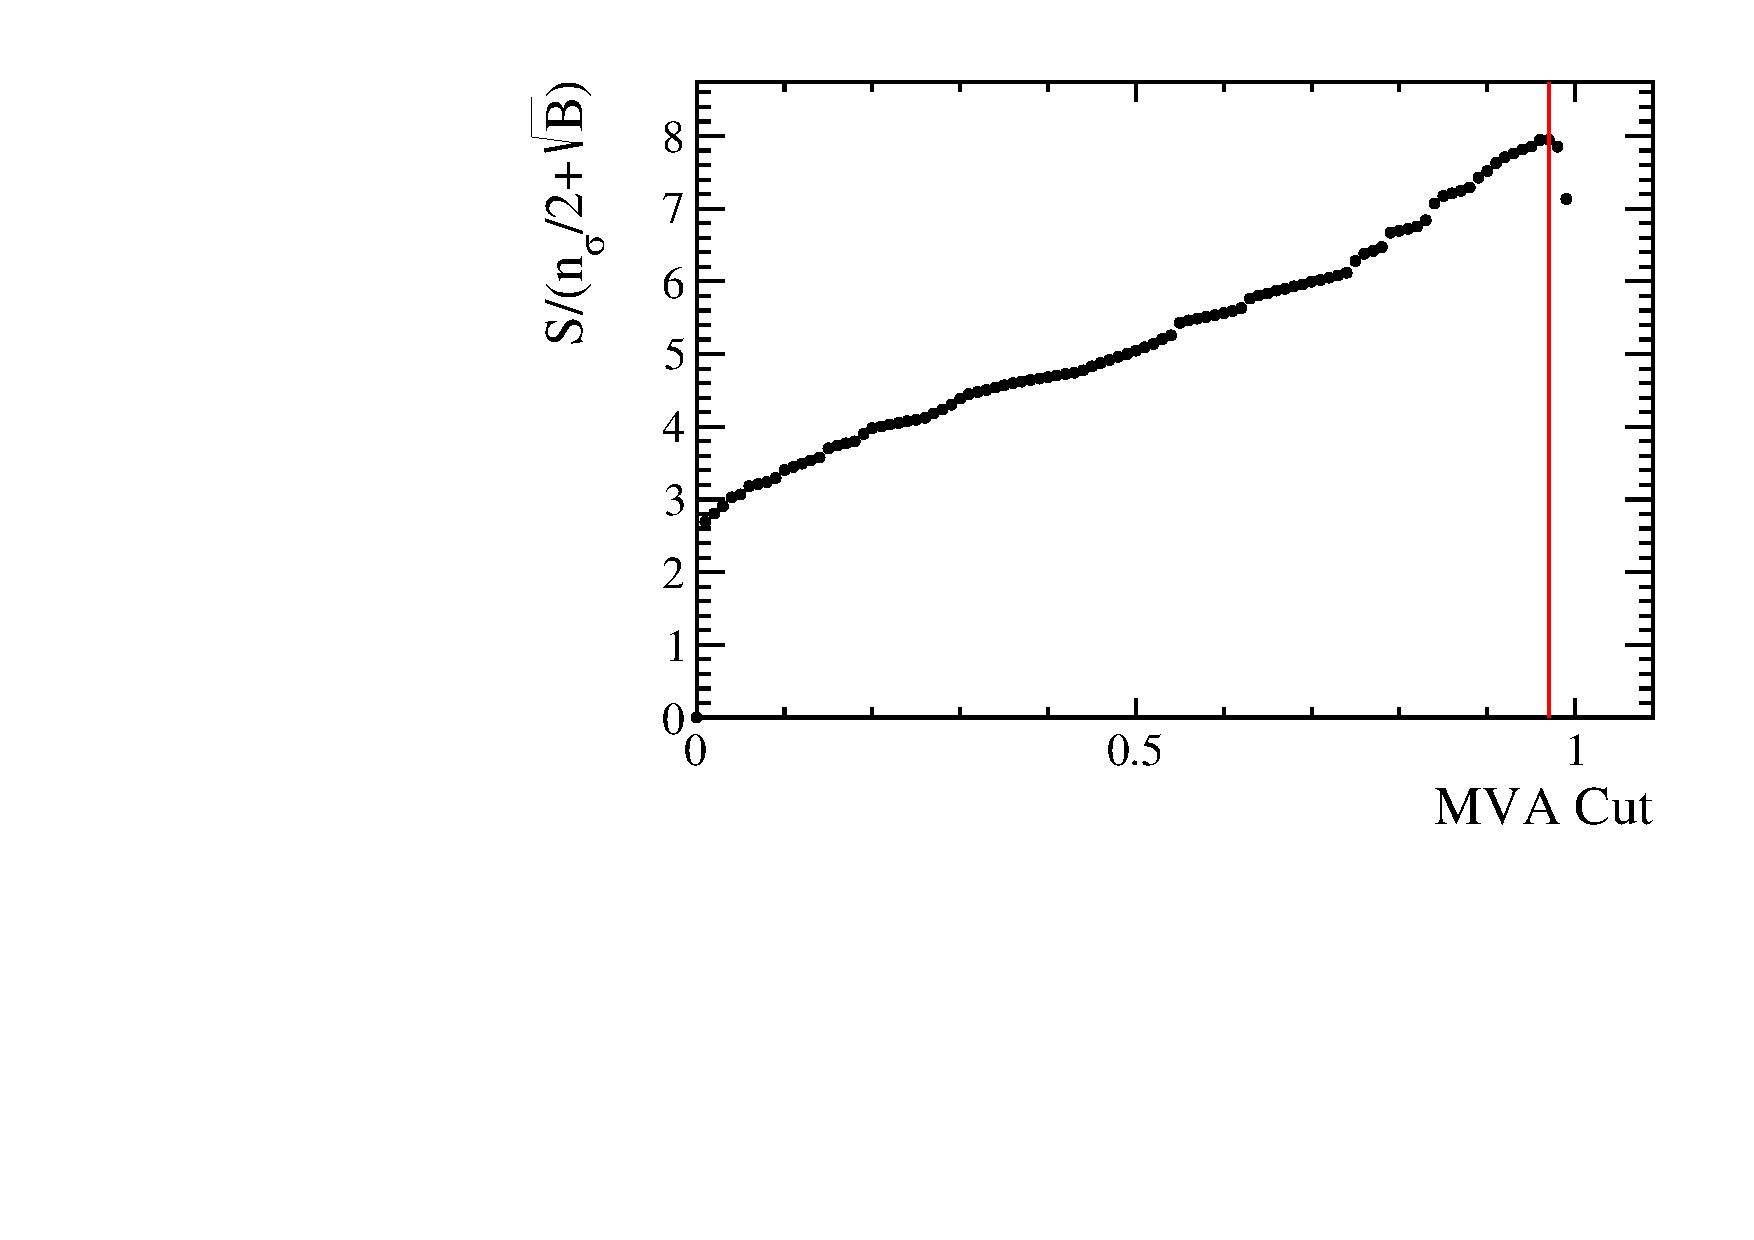
\includegraphics[width=0.49\textwidth]{Lmumu/figs/Lmumu_lowQ2_FoM.pdf}
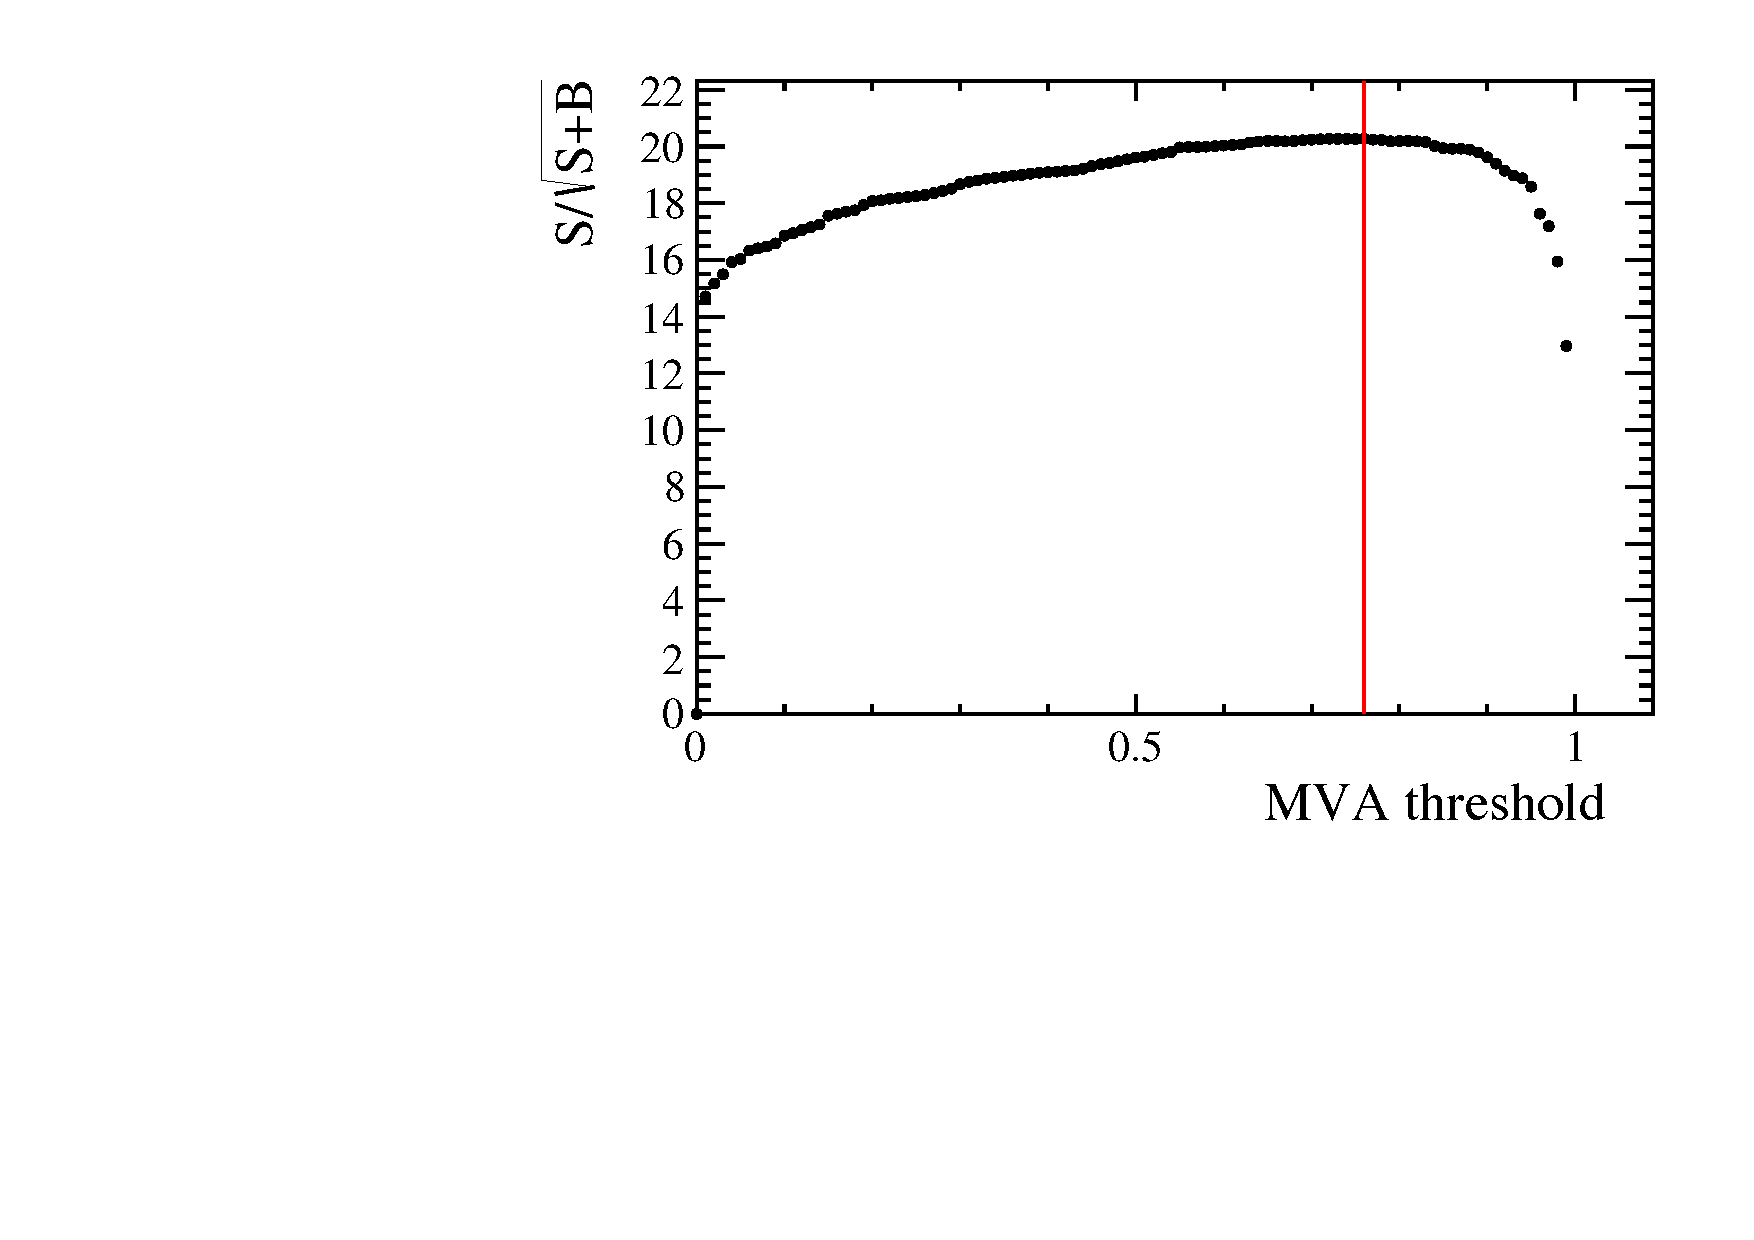
\includegraphics[width=0.49\textwidth]{Lmumu/figs/Lmumu_highQ2_FoM.pdf}
\caption{Dependence of the figure-of-merits on the neural network output requirement for the low-\qsq
(left) and high-\qsq (right) regions. The vertical lines correspond to the chosen cuts.}
\label{fig:Lb_FOM}
\end{figure}
%
\begin{figure}
\centering
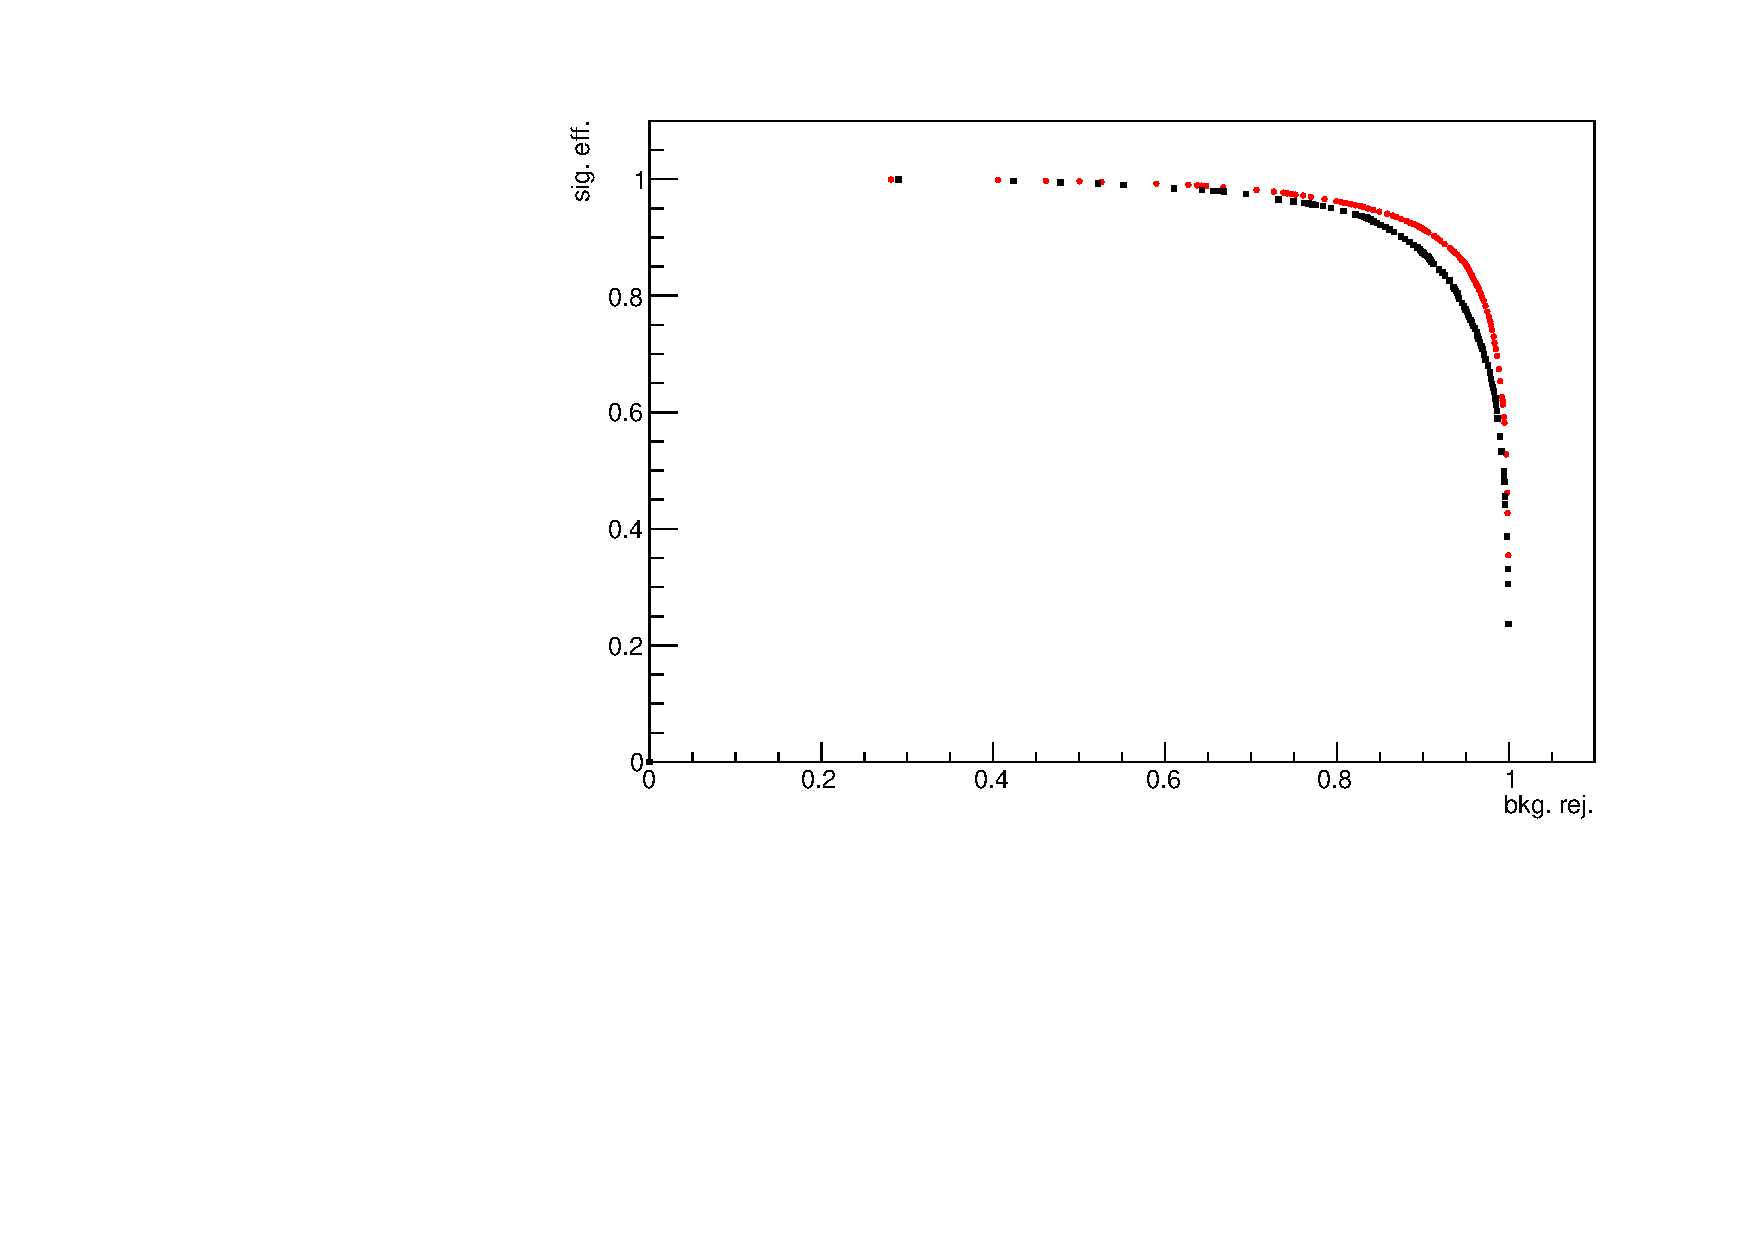
\includegraphics[width=0.7\textwidth]{Lmumu/figs/ROC.pdf}
%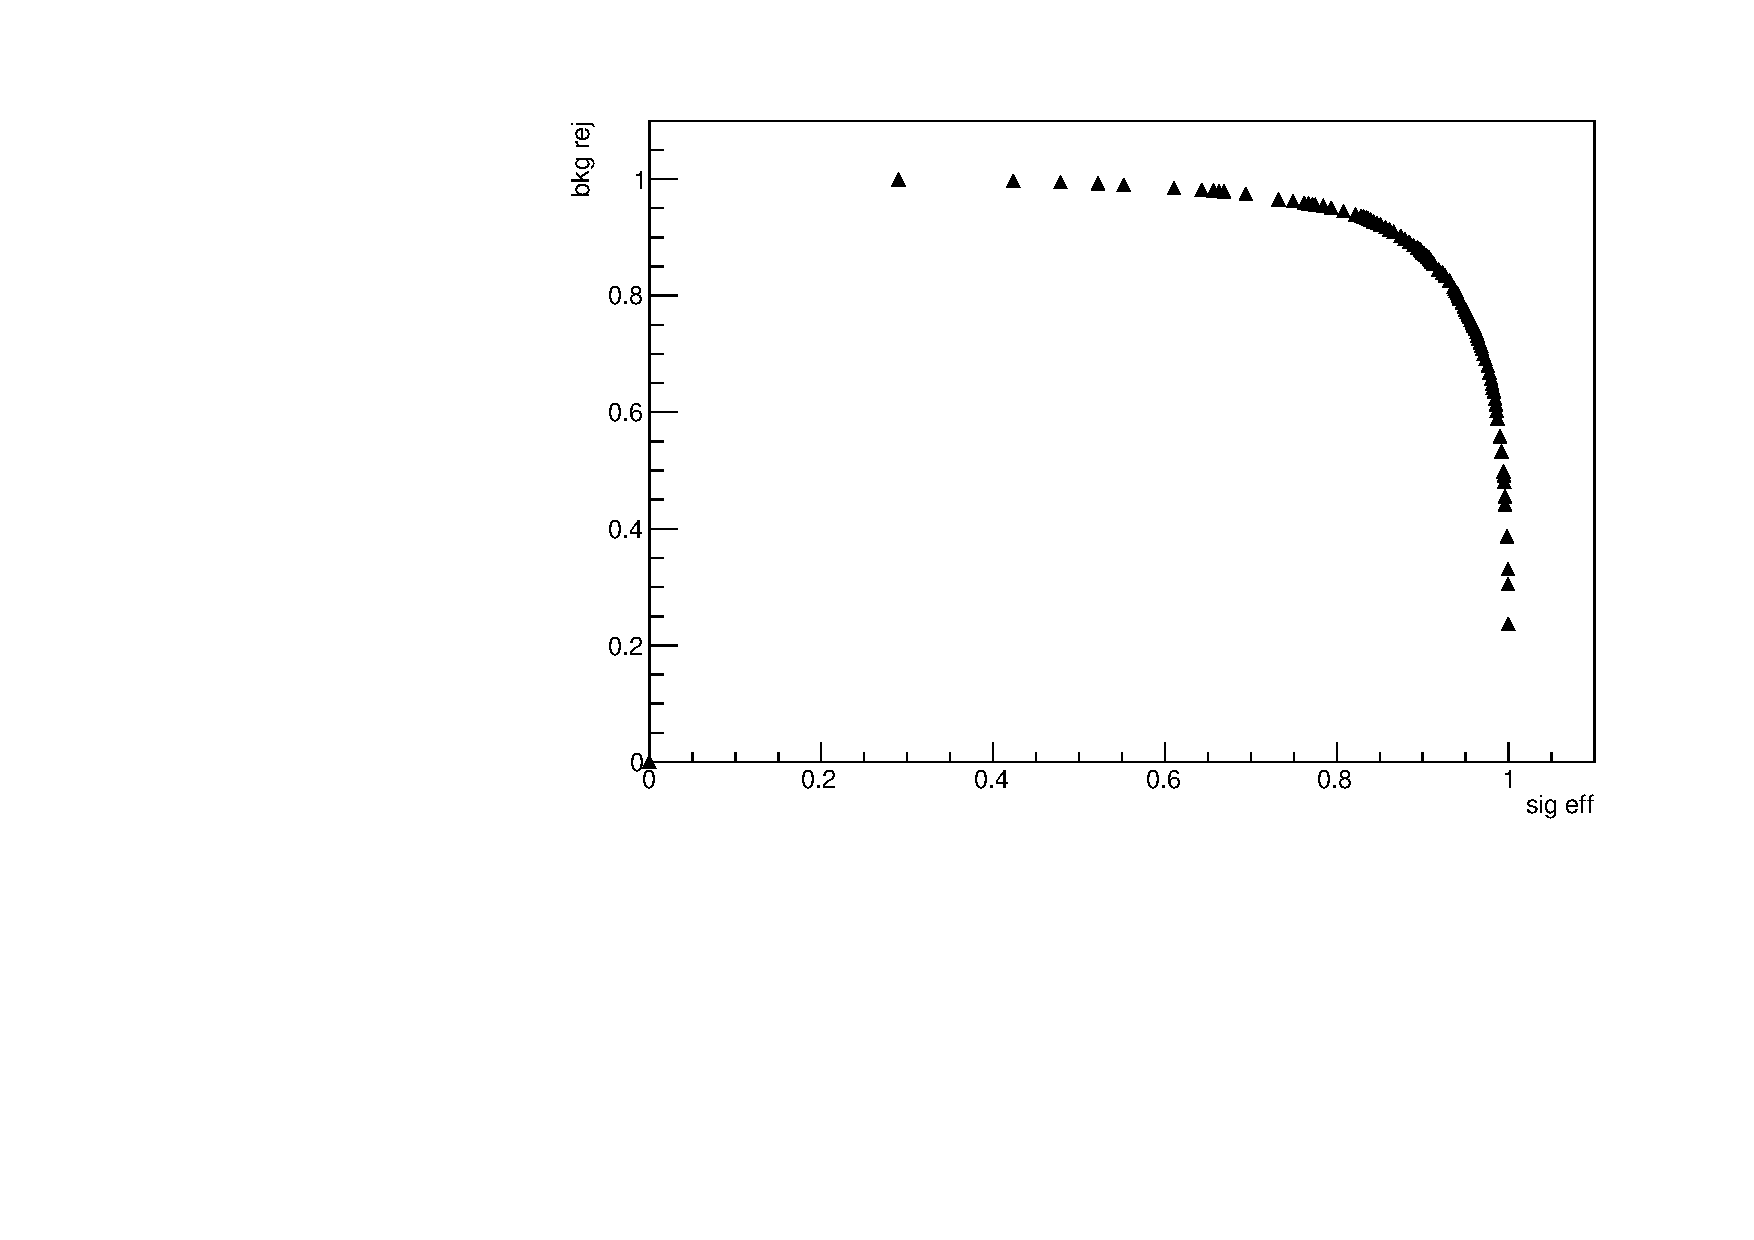
\includegraphics[width=0.48\textwidth]{Lmumu/figs/ROC_Lmumu_highQ2.pdf}
\caption{Receiver operating characteristic (ROC) curves for low-\qsq (black) and high-\qsq (red).
They show the signal efficiency versus the background rejection.
The optimal points on these curves are the closest ones to (1,1). }
\label{fig:Lb_ROC}
\end{figure}

%\begin{figure}
%\centering
%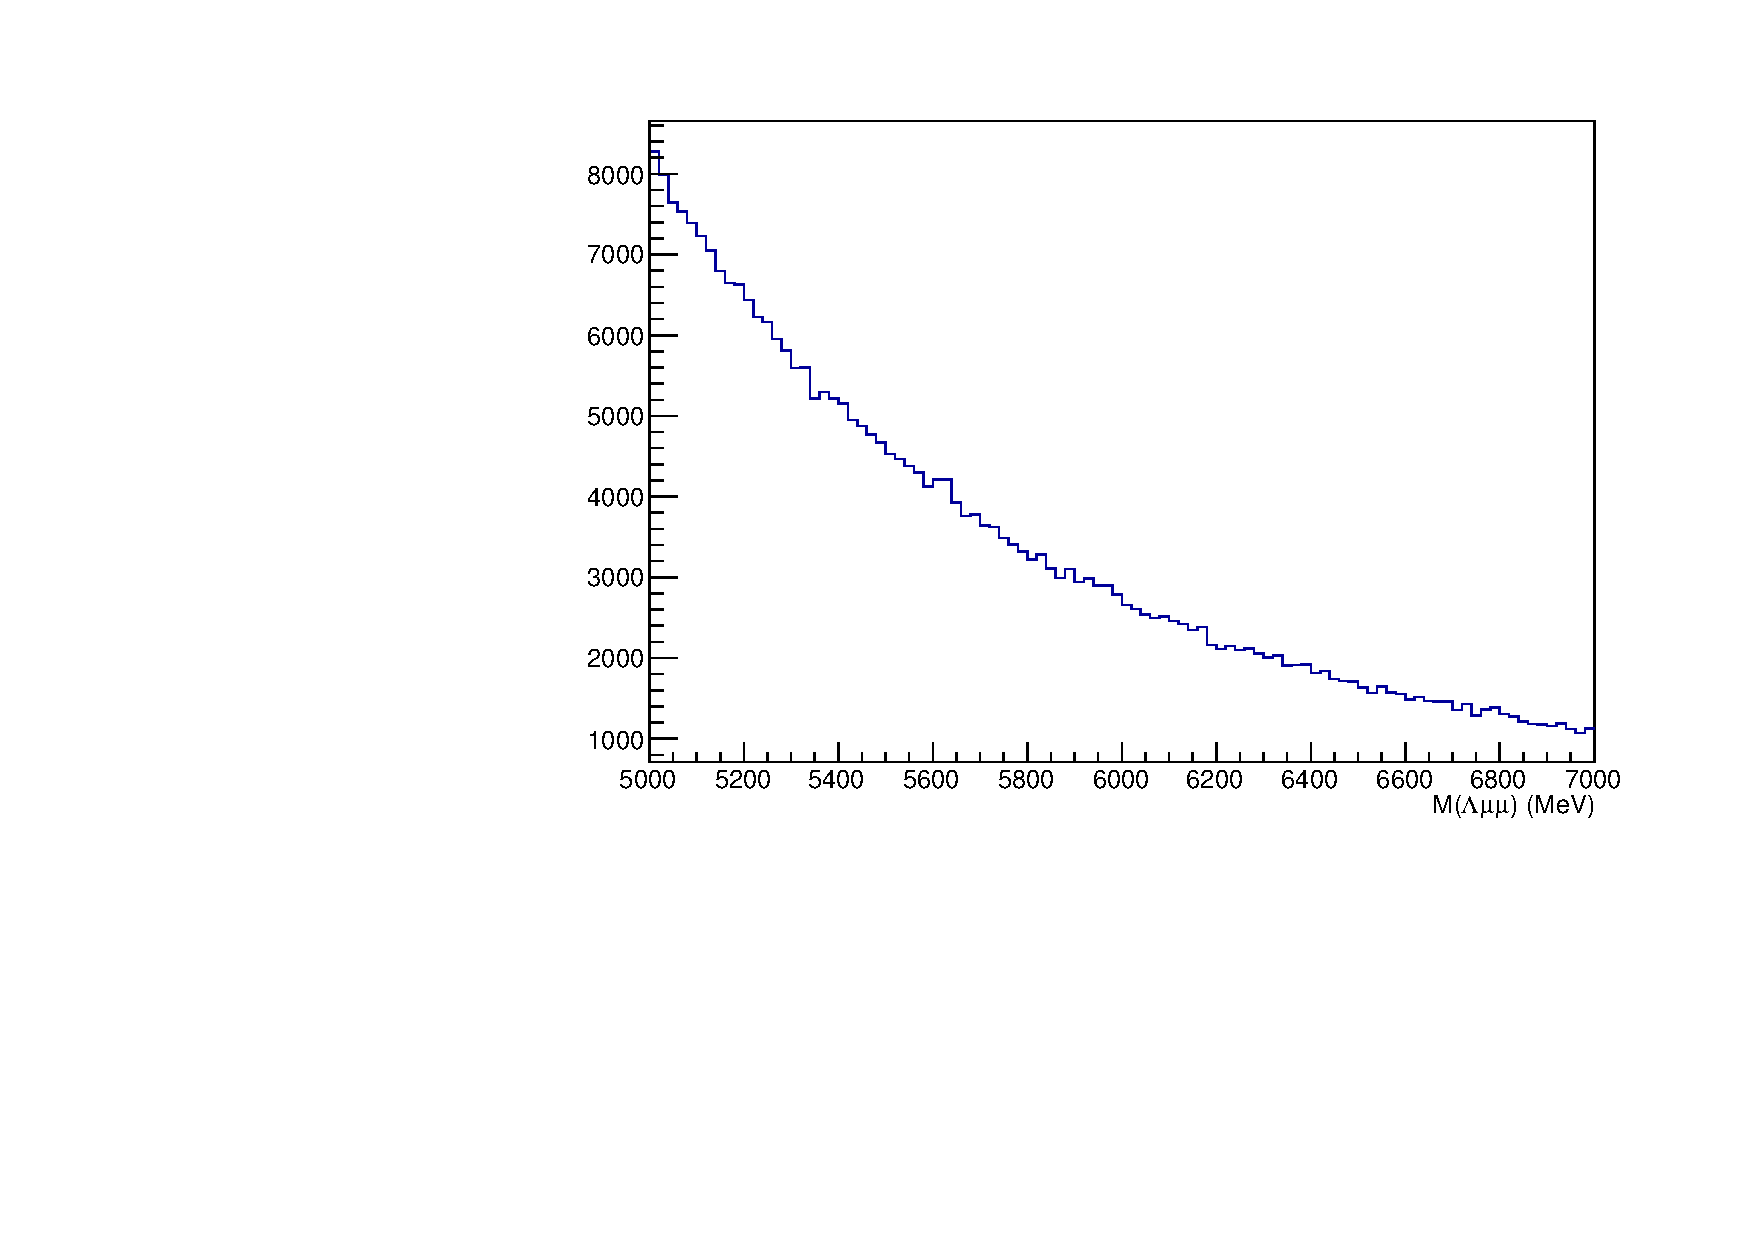
\includegraphics[width=0.48\textwidth]{Lmumu/figs/Lb_MM_beforeMVAcut.pdf}
%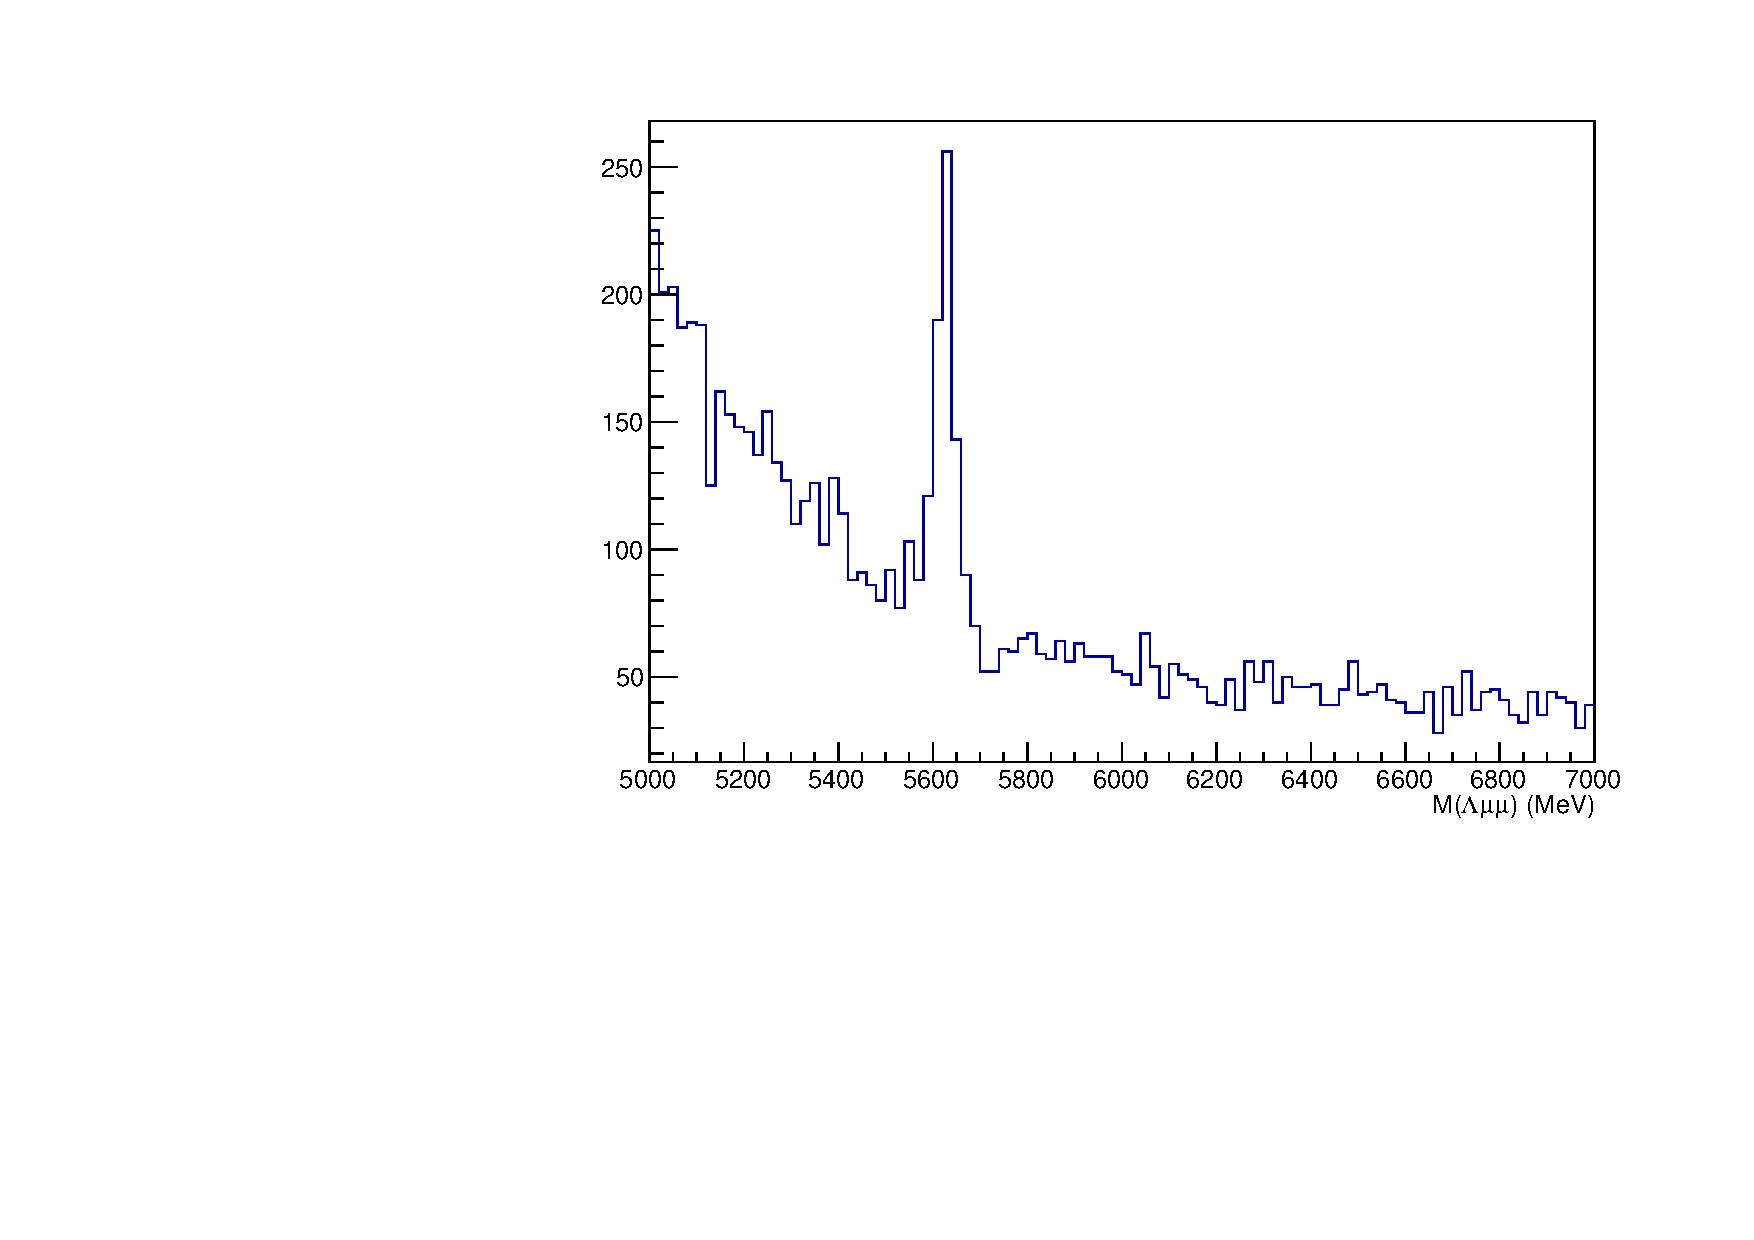
\includegraphics[width=0.48\textwidth]{Lmumu/figs/Lb_MM_afterMVAcut.pdf}
%\caption{Invariant mass distribution $\Lb\to\Lz\mumu$ candidates before the MVA cut (left) and after the cut (right). This plot includes all data
%outside charmonium vetoes.}
%\label{fig:massDists}
%\end{figure}
%
%In Fig.~\ref{fig:massDists} we show invariant mass distributions of rare decay candidates before and after the MVA selection; the plot after MVA corresponds to final selection.
%In Fig.~\ref{fig:L0mass} we show the $m(p\pi)$ invariant mass of selected candidates, peaking at the PDG value for \Lz mass (1115 \mevcc).
%This indicates that our sample is dominated by real \Lz decays.  
%
%\begin{figure}
%\centering
%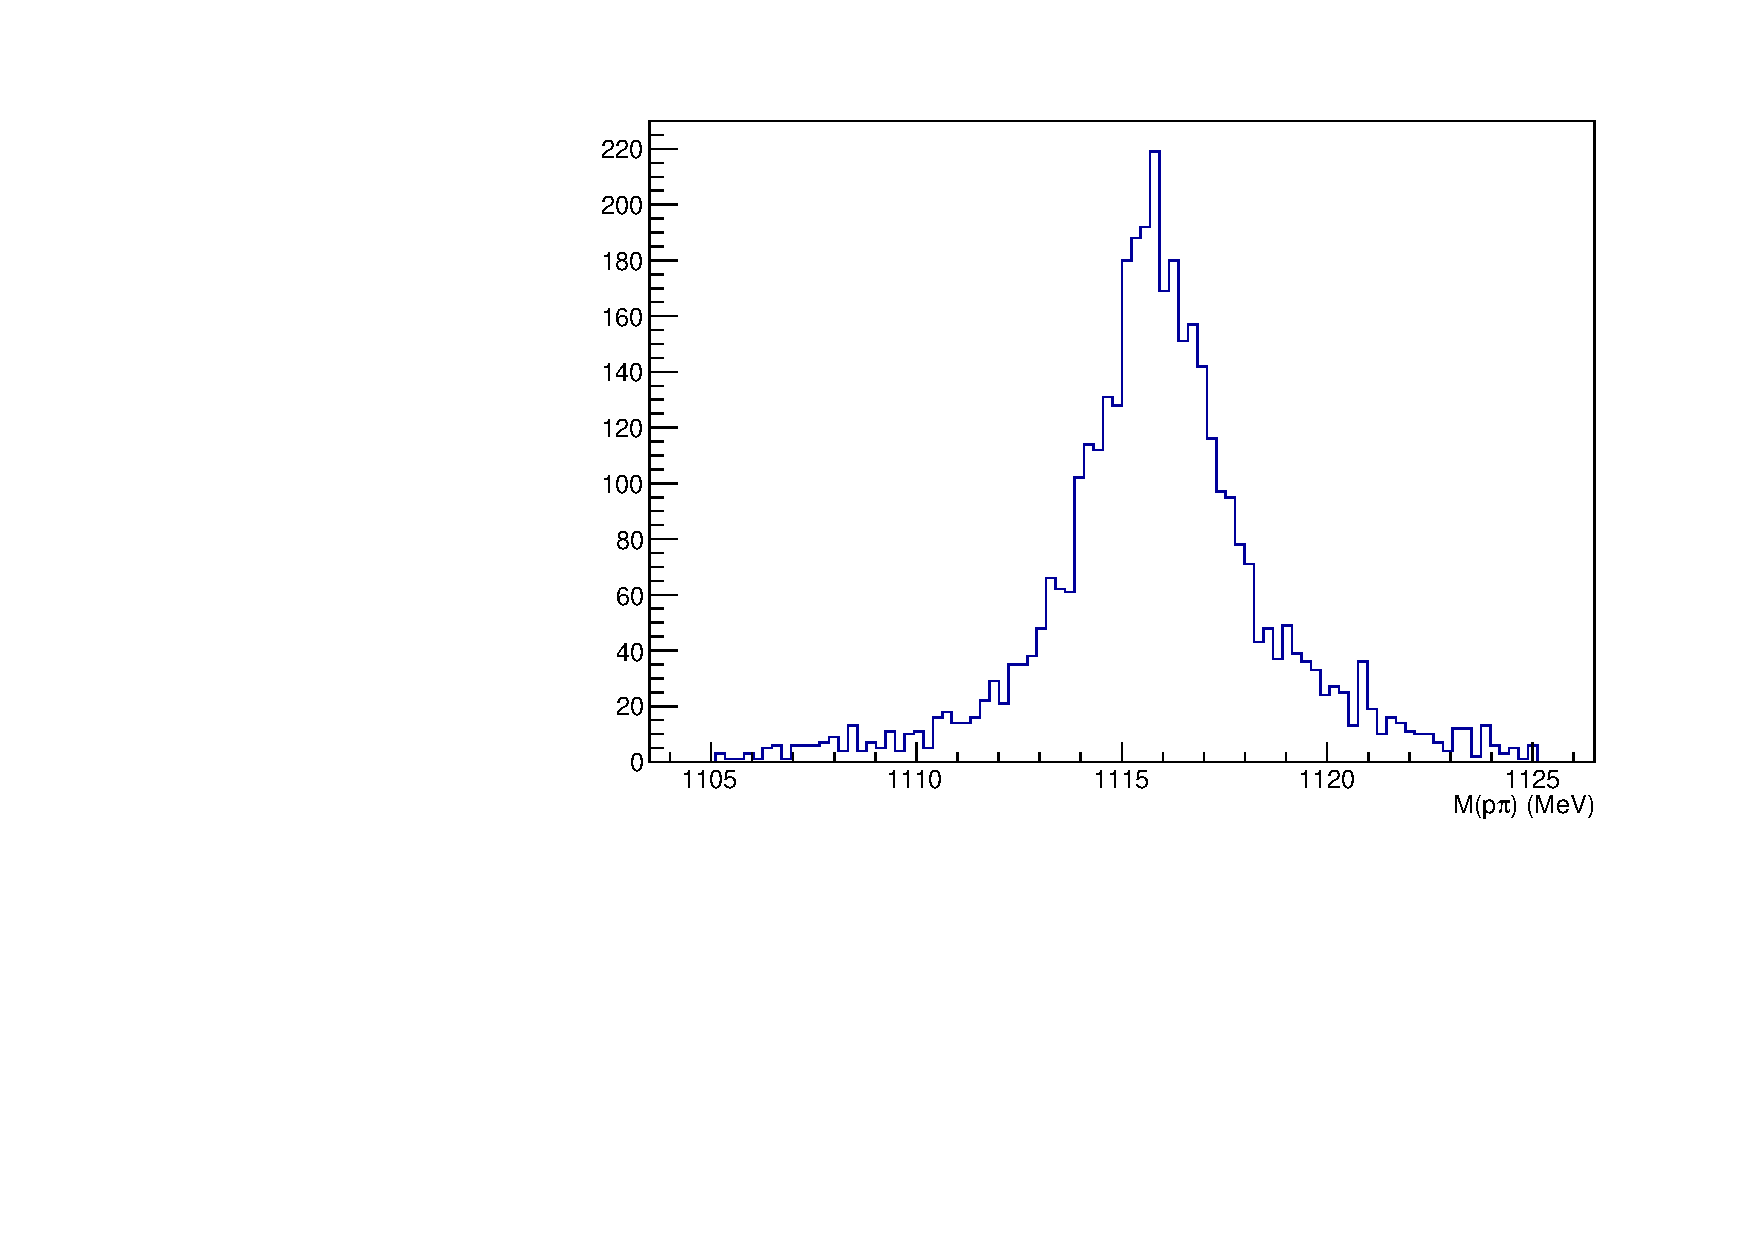
\includegraphics[width=0.7\textwidth]{Lmumu/figs/Lambda0_mass.pdf}
%\caption{Invariant mass $m(p\pi)$ of fully selected candidates.}
%\label{fig:L0mass}
%\end{figure}




\subsection{Trigger}

Specific trigger lines are selected, corresponding to events triggered by the muons
from which the reconstructed candidate is formed. This is denoted as Trigger On Signal (TOS).
The trigger lines used in the analysis are listed in Tab.~\ref{tab:Lb_triggerLines}.
The logical {\em or } of the lines on the same trigger level is required and the logical {\em and}
of those on different levels.
The \verb!L0Muon! trigger requires hits in the muon detector and triggers if a muon with $\pt > 1.5 \gevc$ is identified.
The \verb!L0Dimuon! trigger imposes the same requirement on the sum of the transverse momenta of two tracks.
The \verb!Hlt1TrackAllL0! trigger performs a partial reconstruction of the events and applies basic requirements on the
values of the IP, $\chi^2$ and \pt of tracks; it triggers if the L0 decision is confirmed. The \verb!Hlt1TrackMuon! trigger applies looser requirements 
but in addition requires the \verb!isMuon! variable (see Sec.~\ref{sec:PID_perf}) to be true to limit the yield.
Finally, at the Hlt2 level, a complete reconstruction is done and a multivariate analysis is used to identify decay 
structures. One of the main variables used at this stage is the distance of closest approach, which is 
required to be less than 0.2 mm to form a 2-body object.
%
\begin{table}[h]
\centering
\caption{Summary of the trigger lines used to select events at various levels.
Trigger is always required to be due to the tracks of the candidate itself.}
\begin{tabular}{$l^c} 
	\rowstyle{\bfseries}
Trigger Level &  Lines   \\ \hline
\multirow{2}{*}{L0}            	& \verb!L0Muon!  \\
                				& \verb!L0DiMuon! \\ \hline
\multirow{2}{*}{HLT1}        	& \verb!Hlt1TrackAllL0! \\ 
               				& \verb!Hlt1TrackMuon!      \\ \hline
\multirow{4}{*}{HLT2} 	& \verb!Hlt2Topo[2-4]BodyBBDT!  \\
              				& \verb!Hlt2TopoMu[2-4]BodyBBDT!\\
              				& \verb!Hlt2SingleMuon!     \\
              				& \verb!Hlt2DiMuonDetached! \\ \hline
\end{tabular}
\label{tab:Lb_triggerLines}
\end{table}
%
%Figure~\ref{fig:trigContrib} shows the single trigger efficiency, defined as if each line was alone.
%\begin{figure}
%\centering
%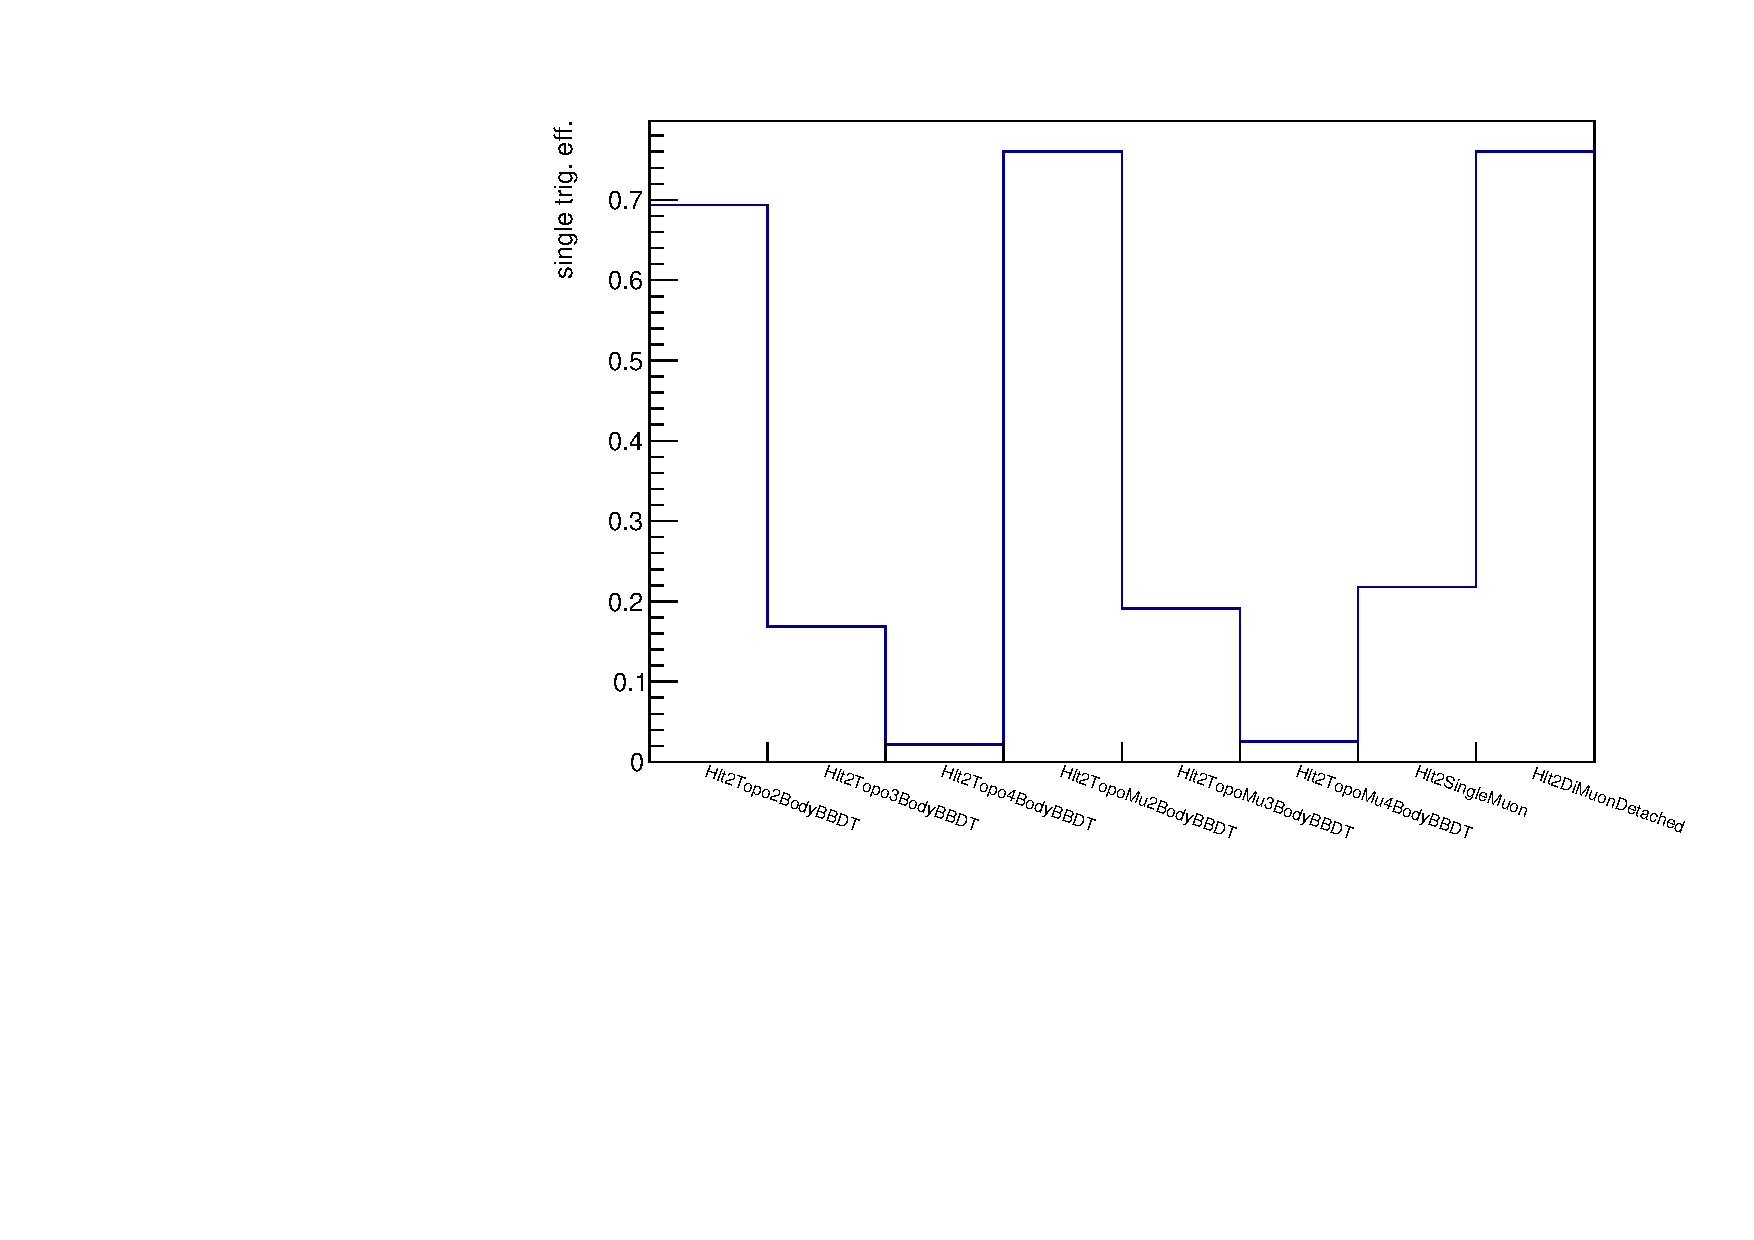
\includegraphics[width=0.48\textwidth]{Lmumu/figs/trig_highq2.pdf}
%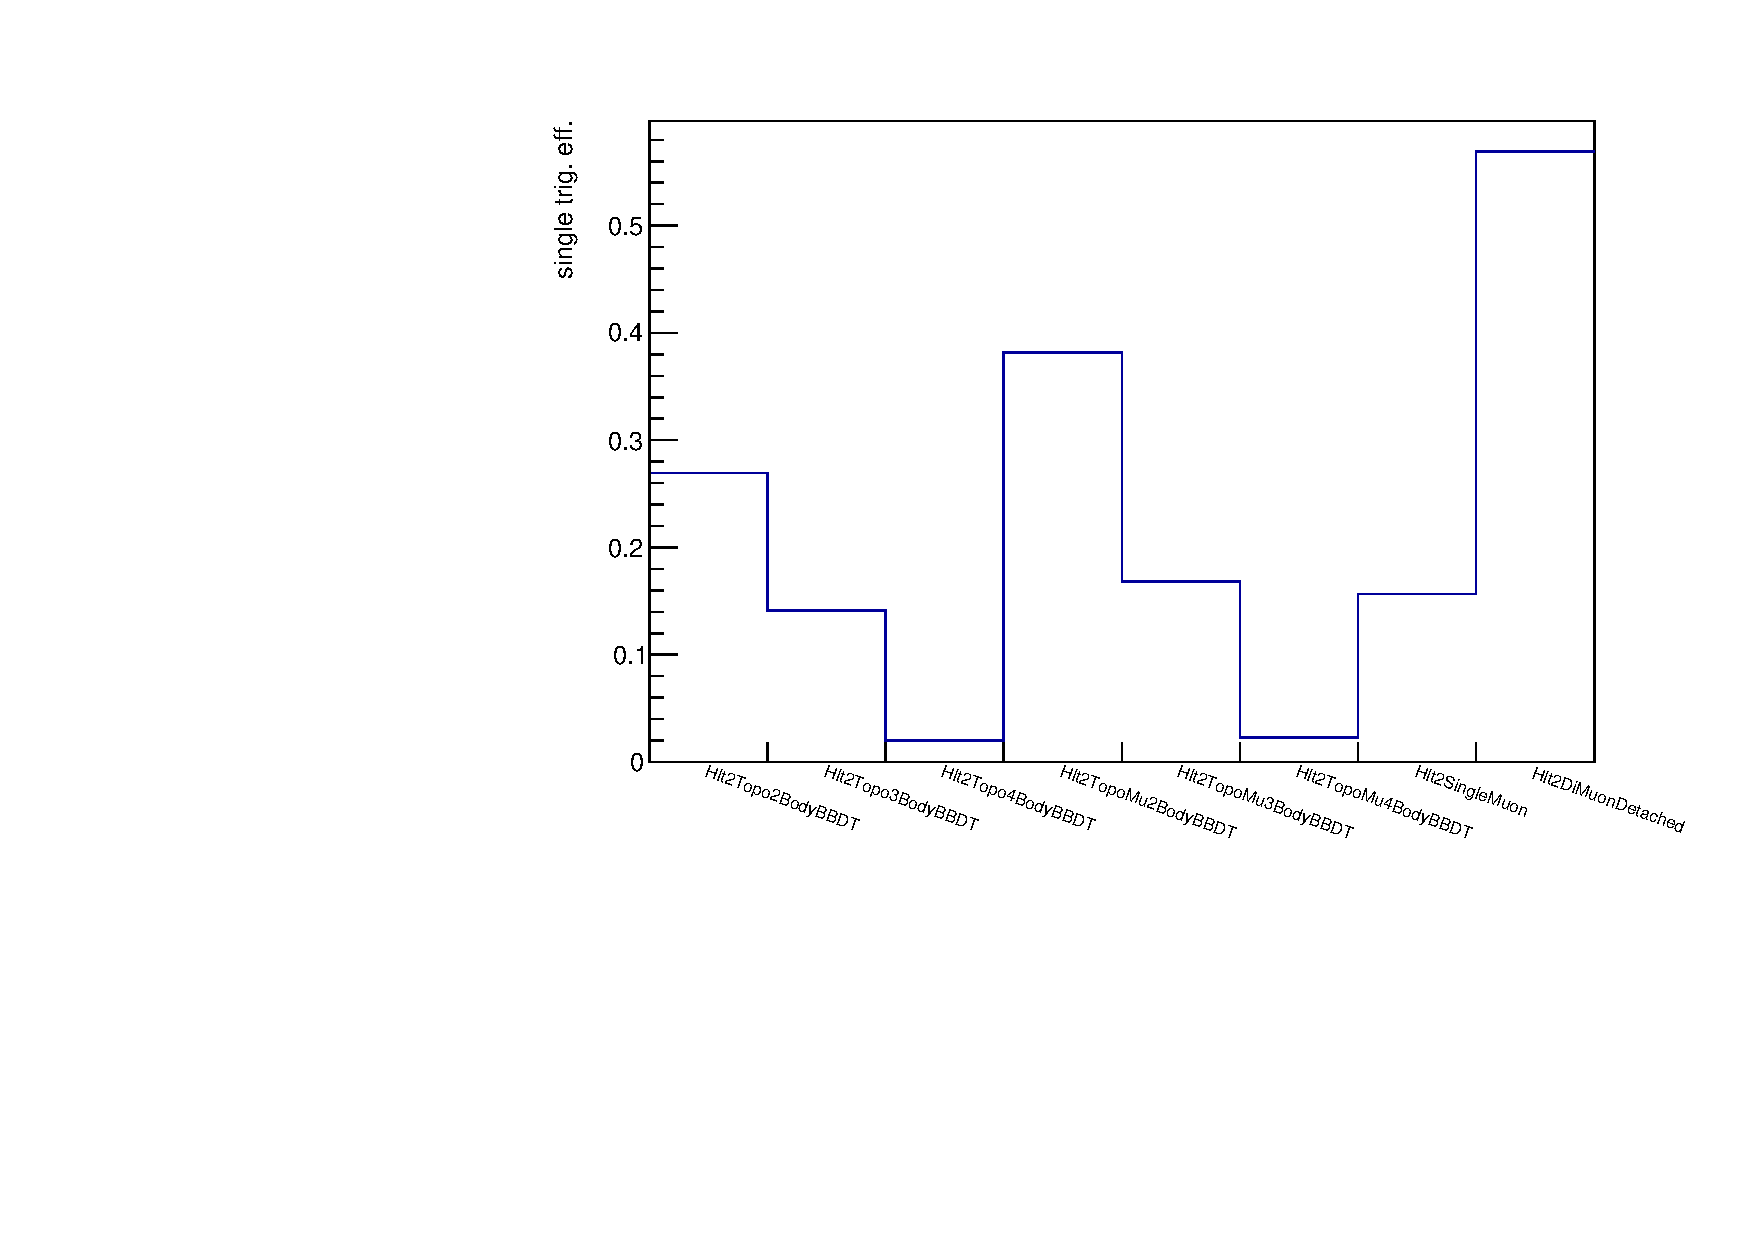
\includegraphics[width=0.48\textwidth]{Lmumu/figs/trig_lowq2.pdf}
%\caption{ Single trigger efficiency for high-\qsq events (left) and low-\qsq (right). }
%\label{fig:trigContrib}
%\end{figure}


\subsection{Background from specific decays}

Candidates from other decays can be incorrectly reconstructed as the decays of interest if
some of their particles escape detection or are mis-identified.
A survey of possible backgrounds concluded that the only physics background
that needs to be taken into account explicitly comes from misreconstructed decays of \Bz to \KS with
two muons in the final state, where the \KS is incorrectly reconstructed 
as a \Lz due to a $p\rightarrow \pi$ identity swap.
% and $m(p\pi)$ in the \Lz mass window. 
The lack of background from other decays is
mainly due to the distinctive topology of the \Lz decay, which is long-lived and decays at a displaced vertex.

Simulated samples are used to study the effect of misreconstructed $\Bz\ra\jpsi\KS$ and $\Bz\ra\KS\mumu$ decays. 
In data, the $\Bz\ra\jpsi\KS$ contribution is clearly visible in the mass distribution of the resonant channel.
This background is not suppressed by the application of specific cuts in this analysis because its mass shape is sufficiently 
distinct the from \Lb signal and its contribution can be reliably modelled in the mass fits (see Sec.~\ref{sec:Lb_fit}).
An approximate estimate of the \KS background level for the rare mode is obtained using the yield in the resonant channel
rescaled by the ratio of the known rare and resonant branching fractions.
Details are given in Sec.~\ref{sec:Lb_fit} and predicted numbers of candidates are reported in Tab.~\ref{tab:KSprediction}.
This contribution, although essentially negligible, is considered in the fit.
The possible contamination due to $B^{+} \ra\mumu K^{*+}$ decays, where the $K^{*+}\to\KS\pi$, is also 
investigated using a dedicated simulated sample and found to be negligible.

Finally, $\Lb\ra\jpsi\Lz$ events 
%radiating photons from the final state, can escape the \jpsi veto and be 
in which a photon is radiated from one of the muons in the \jpsi decay, may be reconstructed 
with the wrong \qsq value, avoid the \jpsi veto and hence be 
reconstructed in the rare channel sample. By analysing simulated events it was found that 
such radiative candidates only contribute in the \qsq interval $6 < \qsq < 8$~\gevgevcccc.
Of the $\Lb\to\jpsi\Lz$ candidates 1.3\%  are reconstructed in this \qsq interval but only 0.06\%
fall into the 4-body invariant mass window used for the fits. This corresponds to $\sim 6$
candidates, 4 of which are in the downstream category. Given the low yield and that these candidates do
not peak under the signal but show a decaying distribution at the edge of the fit mass window, this
background is considered as part of the combinatorial background.
%Given that this contribution does not contribute in the region where we expect \Lb peak, we do
%not attempt to exclude this but it is again modelled in the fit.
Figure~\ref{fig:peakingBkgs} shows the 4-body invariant mass distribution of simulated $\Lb\ra\jpsi\Lz$
events falling into the rare \qsq region and the distribution of simulated $B^{+} \ra\mumu K^{*+}$
events misreconstructed as $\Lb\ra\jpsi\Lz$ decays.
%
\begin{figure}
\centering
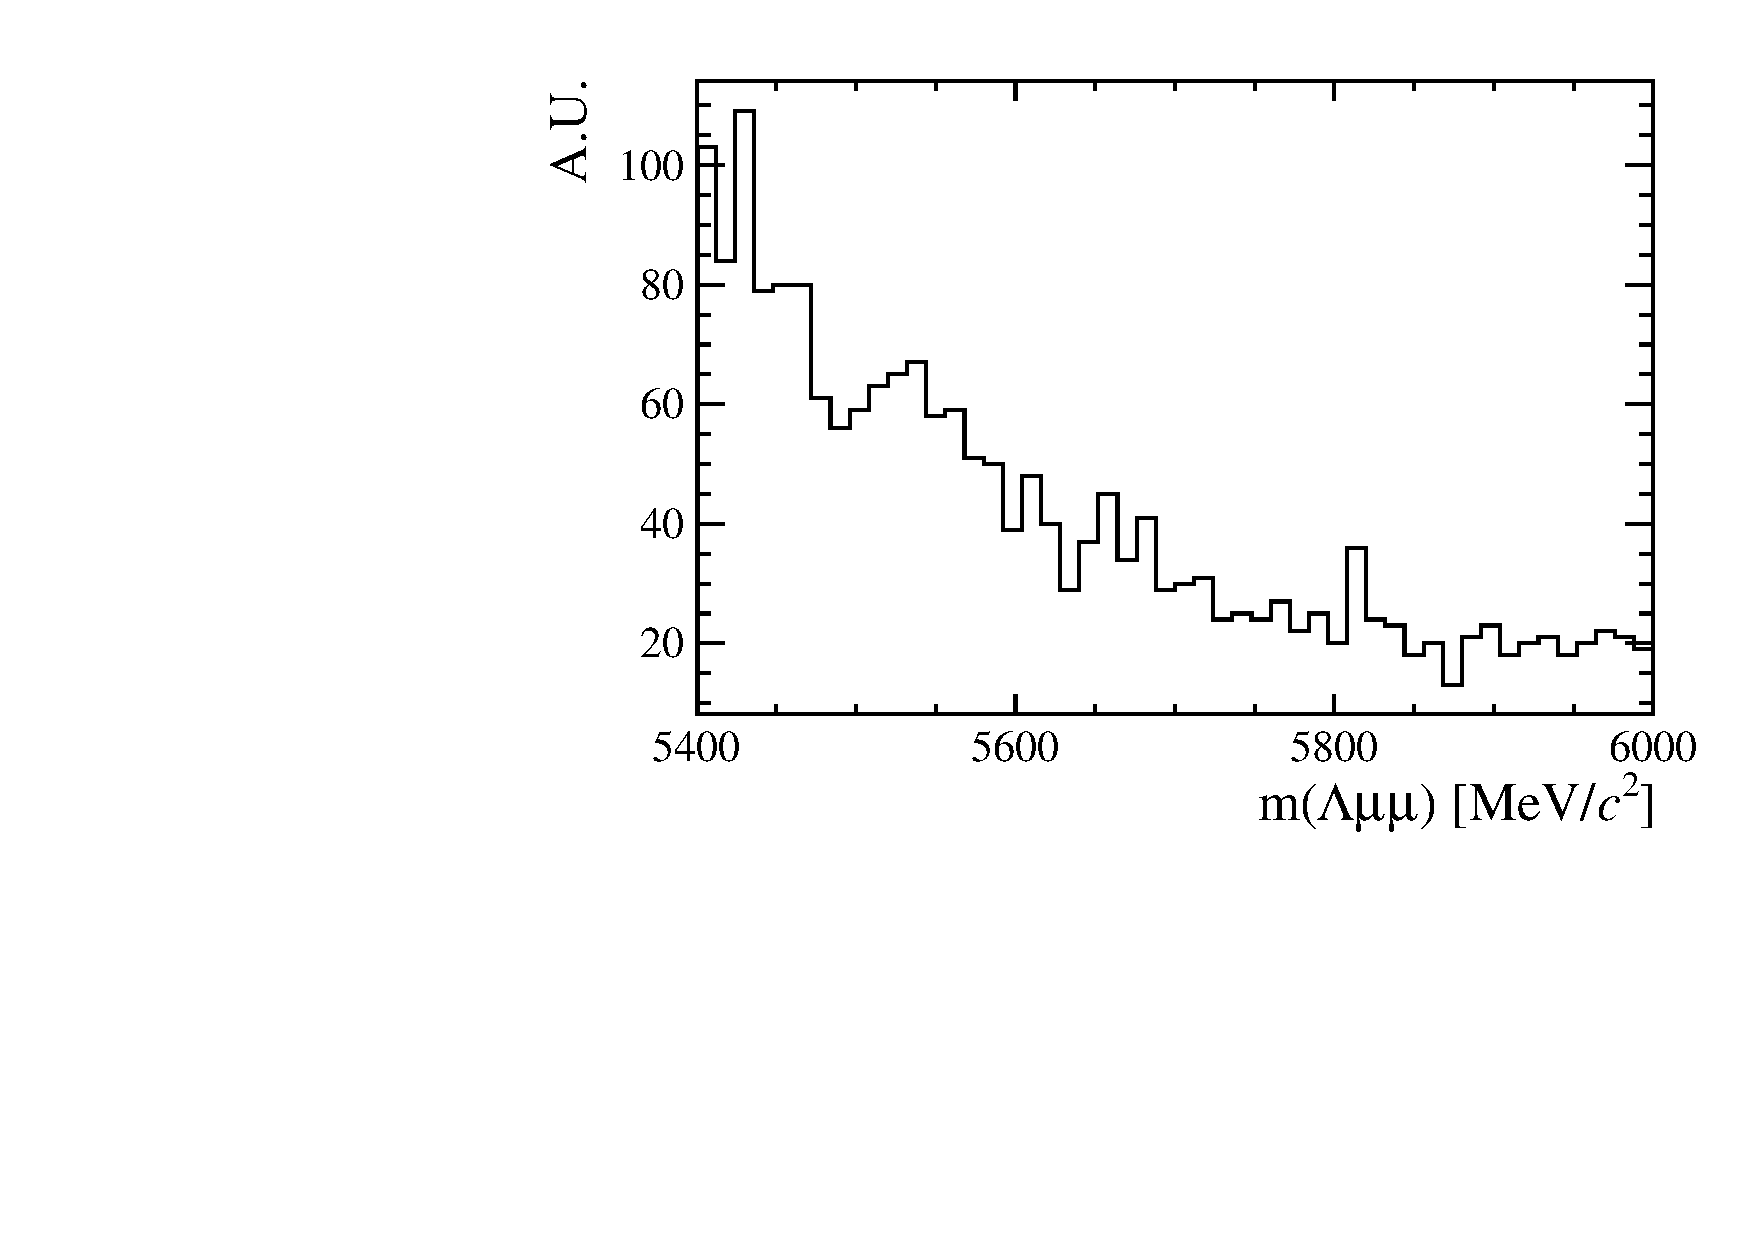
\includegraphics[width=0.49\textwidth]{Lmumu/figs/Bu2Kstplus_mass.pdf}
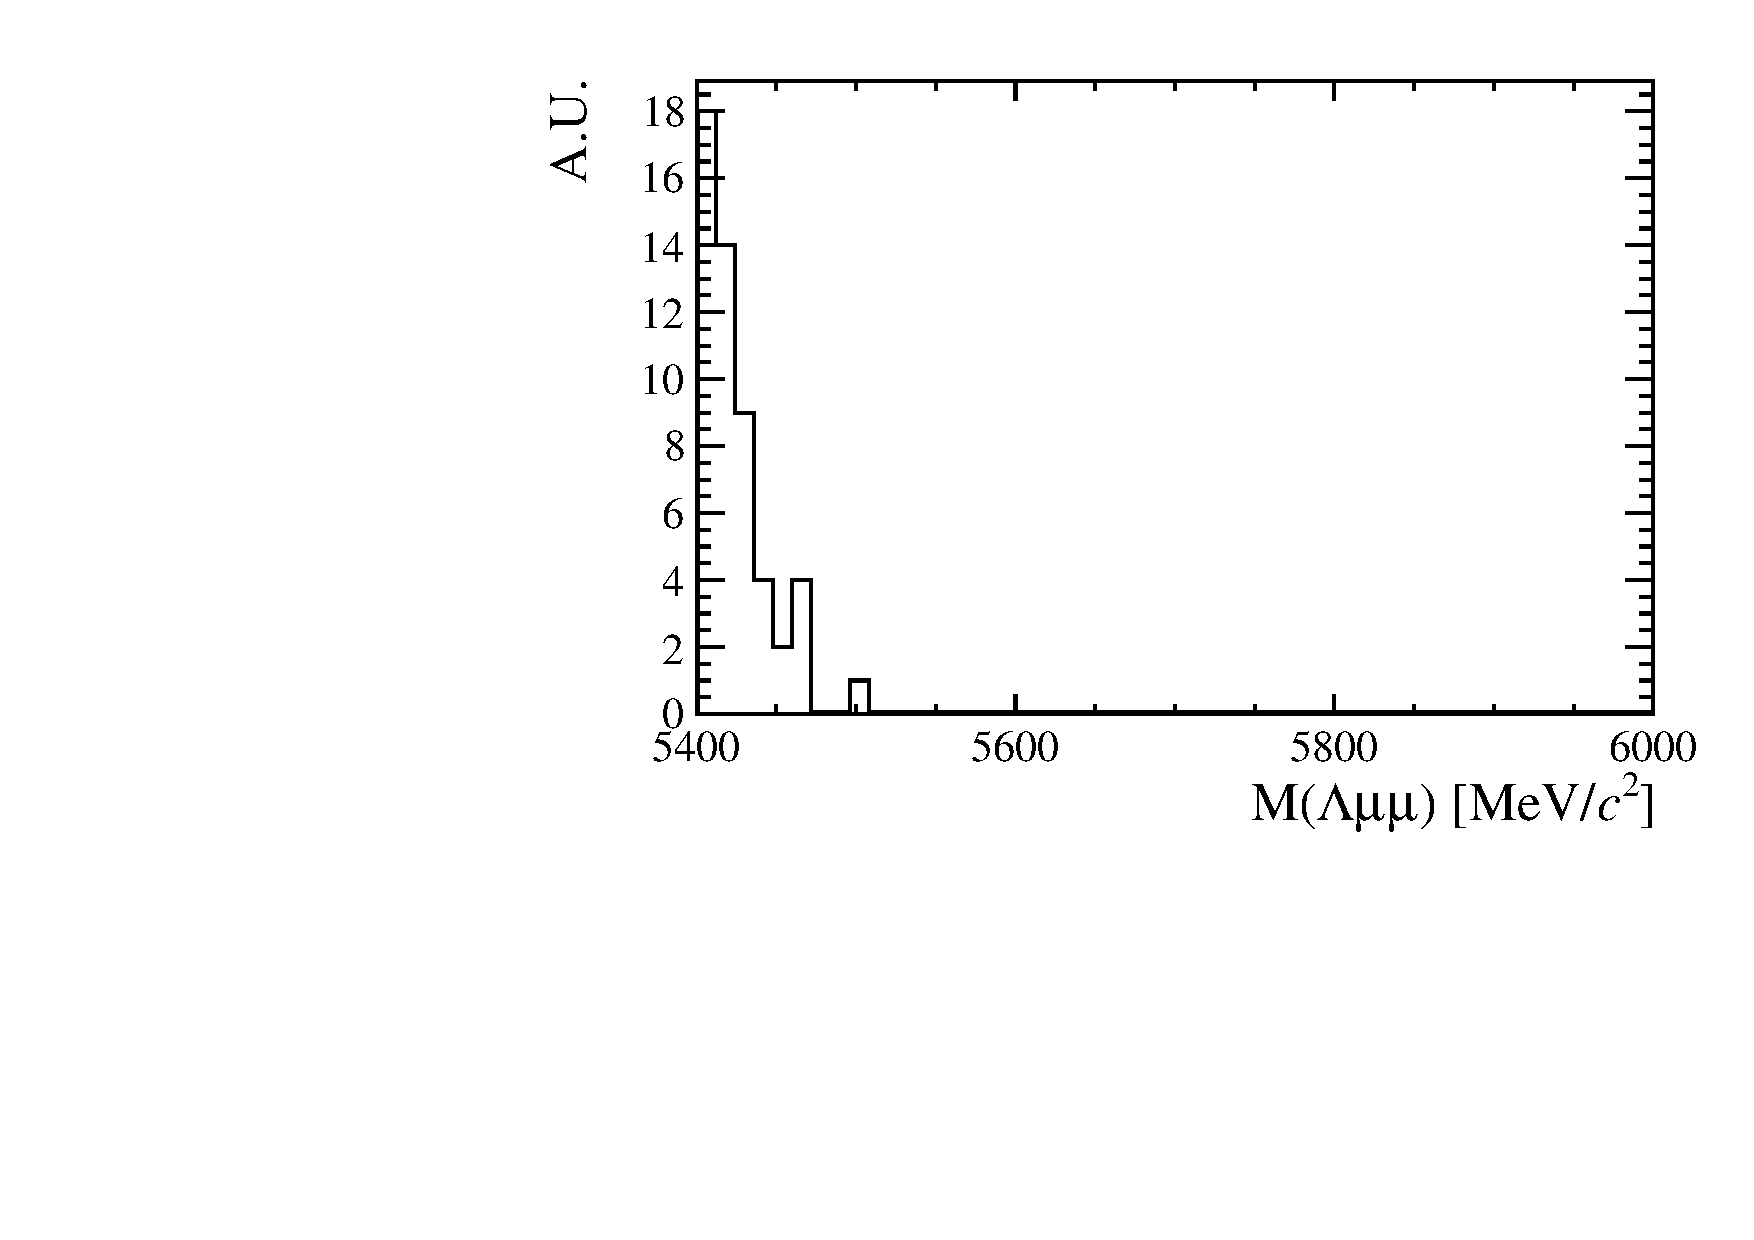
\includegraphics[width=0.49\textwidth]{Lmumu/figs/JpsiL_leakage_mass.pdf}
\caption{ Invariant mass distributions of simulated $B^{+} \ra\mumu K^{*+}$ (left)
and \Lb\to\jpsi\Lz (right) candidates passing the full $\Lz\mu\mu$ selection. Only \Lb\to\jpsi\Lz
candidates reconstructed in $\qsq < 8$ \gevgevcccc are selected.
Distributions are shown in the invariant mass range relevant for the analysis 
(see Sec.~\ref{sec:Lb_fit}). }
\label{fig:peakingBkgs}
\end{figure}


\section{Yield extraction}

Extended unbinned maximum likelihood fits are used to extract the yields of the rare and resonant channels.
The likelihood has the form:
%
\begin{equation}
\mathcal{L}=e^{-(N_\mathrm{S}+N_\mathrm{C}+N_{\mathrm{B}})}\times\prod_{i=1}^{N}\left[
N_\mathrm{S}P_{\mathrm{S}}(m_i)+N_\mathrm{C}P_\mathrm{C}(m_i)+N_{\mathrm{B}}P_{\mathrm{B}}(m_i)\right]
\end{equation}
\noindent
where $N_\mathrm{S}$, $N_\mathrm{C}$ and $N_\mathrm{B}$ are respectively the numbers of signal, 
combinatorial and \KS background candidates and the $P_i(m_i)$ are the corresponding probability density functions (PDF).
The fit variable is the 4-body $m(p\pi\mu\mu)$ invariant mass obtained from
a kinematical fit of the full decay chain in which each particle is constrained to point to its
assigned origin vertex and the invariant mass of the $p\pi$ system is constrained to be equal to
the world average for the \Lz baryon mass. In the resonant case a further constrain is used on the dimuon
mass to be equal to the known \jpsi mass. This method allows to improve the mass resolution giving
better defined peaks and therefore a more stable fit. For brevity, in the following these variables are
simply referred to as ``invariant mass".

\subsection{Fit description}
\label{sec:Lb_fit}

The fit is performed though the following steps:
%
\begin{itemize}
\item simulated distributions are fit to extract initial parameters;
\item the resonant data sample is fitted;
\item the rare sample is fitted fixing some parameters to those obtained in the previous cases.
\end{itemize}
%

In the first step simulated $\Lb\to\jpsi\Lz$ distributions are fitted using the signal PDF alone.
This is done separately for downstream and long candidates. Figure~\ref{fig:Lb_jpsiMCfit} shows 
distributions of candidates selected in the resonant sample with the fit function overlaid.
%
The signal is described as the sum of two Crystal Ball functions (CB) with
common mean ($m_0$) and tail slope ($n$). This is also known as Double Crystal Ball (DCB) function.
A single Crystal Ball~\cite{Skwarnicki:1986xj} is a probability
density function commonly used to model processes involving energy loss. In particular it is used
to describe resonances' peaks with radiative tails. This function 
consists of a Gaussian core and a power-law tail below a certain threshold and has form
%
\begin{equation}
C(x;\alpha,n,\bar{x},\sigma) = N \cdot
\begin{cases}
exp \left( -\frac{(x - \bar{x})^2}{2\sigma} \right)  & \mbox{   if   } \frac{(x - \bar{x})}{\sigma} > \alpha, \\
A\left( B - \frac{(x - \bar{x})}{\sigma} \right)^{-n} & \mbox{   if   } \frac{(x - \bar{x})}{\sigma} < \alpha,
\end{cases}
\end{equation}
%
where for normalisation and continuity
%
\begin{equation}
\label{CB}
\begin{array}{ll}
A = \left( \frac{c}{|\alpha|} \right))^n \cdot exp(- \frac{\alpha^2}{2}), \\
B = \frac{n}{|\alpha|} - |\alpha|.
\end{array}
\end{equation}
%
The full PDF for the resonant channel is therefore:
%
\begin{equation}
P_\mathrm{S}(m;m_0,\alpha_1,\alpha_2,f,n) = f \cdot \text{CB}(m;m_0,\sigma_1,\alpha_1,n)+(1-f)\text{CB}(m;m_0,\sigma_2,\alpha_2,n),
\end{equation}
%
where $f$ is the relative fraction of candidates falling into the first CB function.

\begin{figure}
\centering
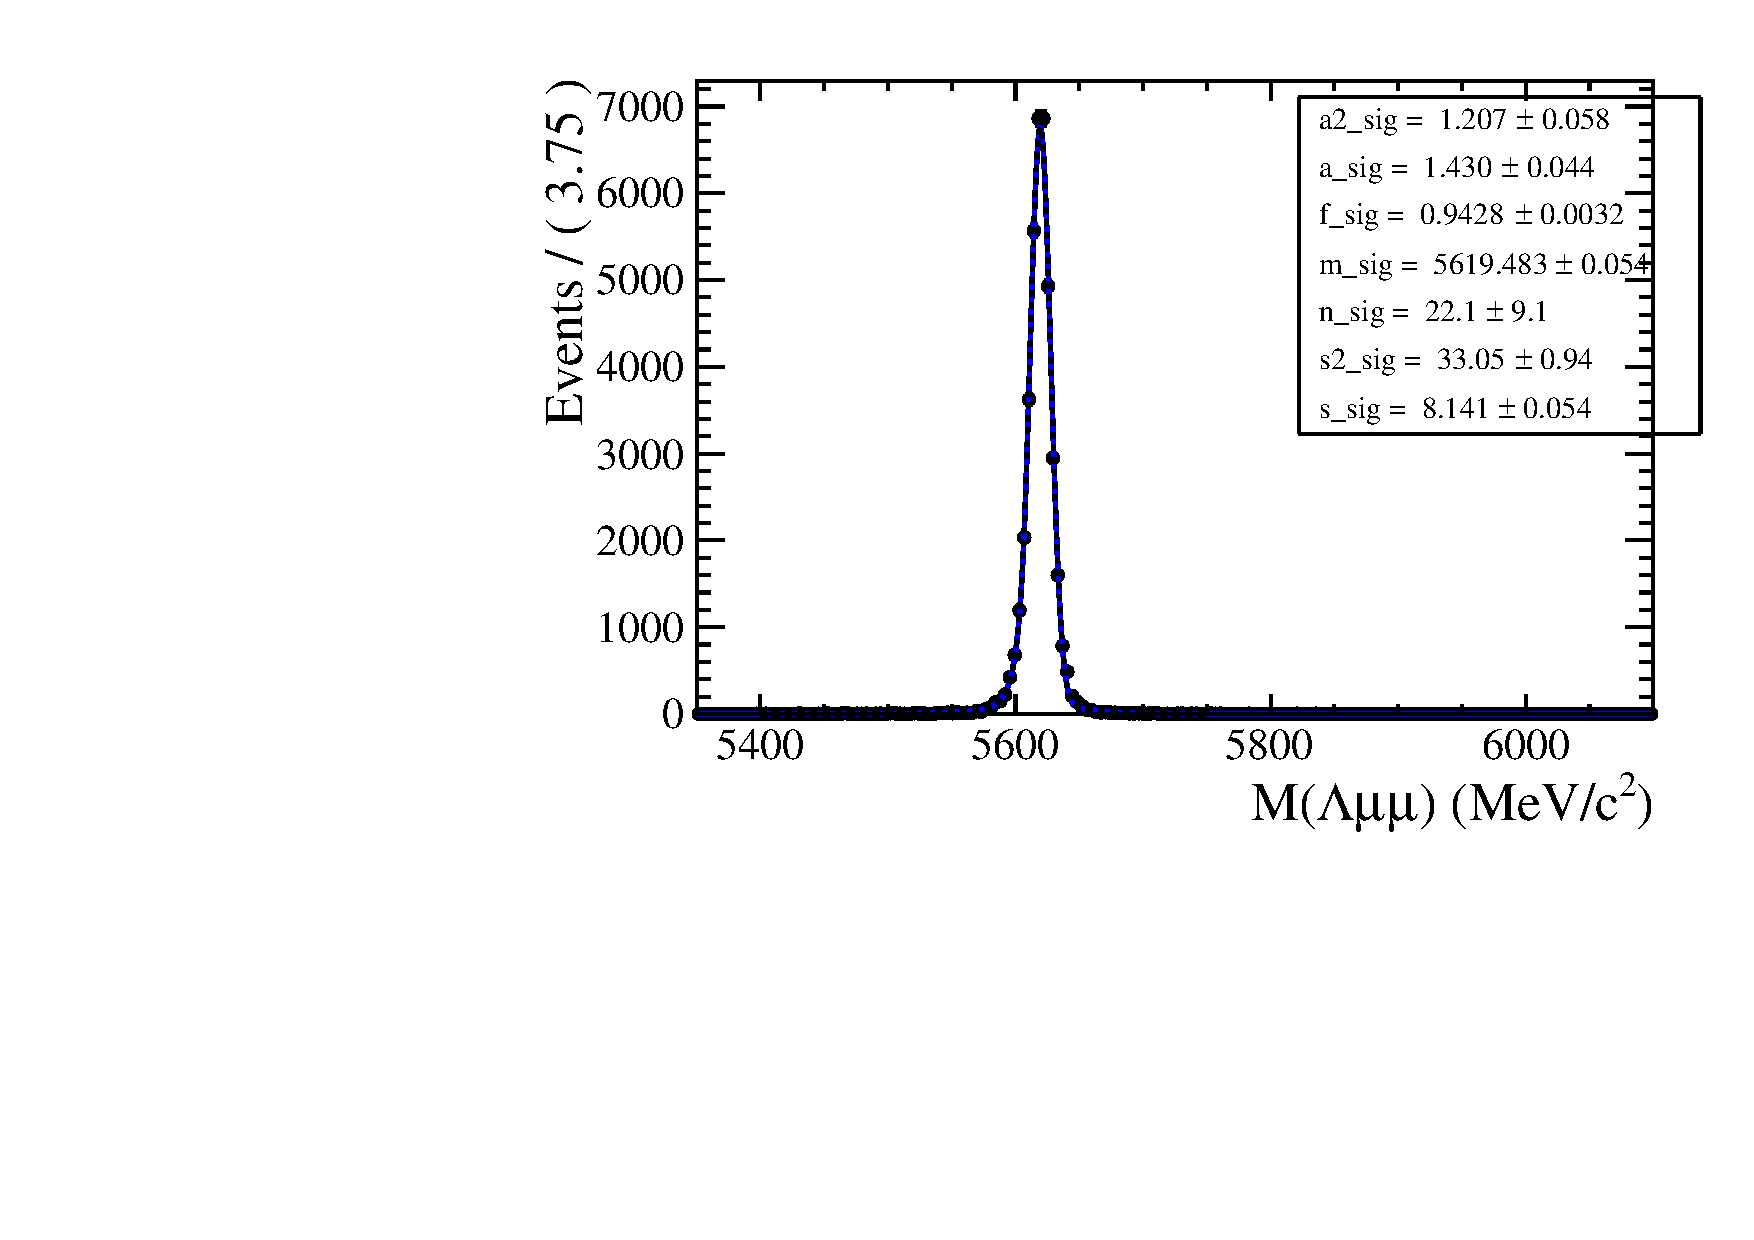
\includegraphics[width=0.49\textwidth]{Lmumu/figs/MassFits/fitLb2JpsiL_DD_MC.pdf}
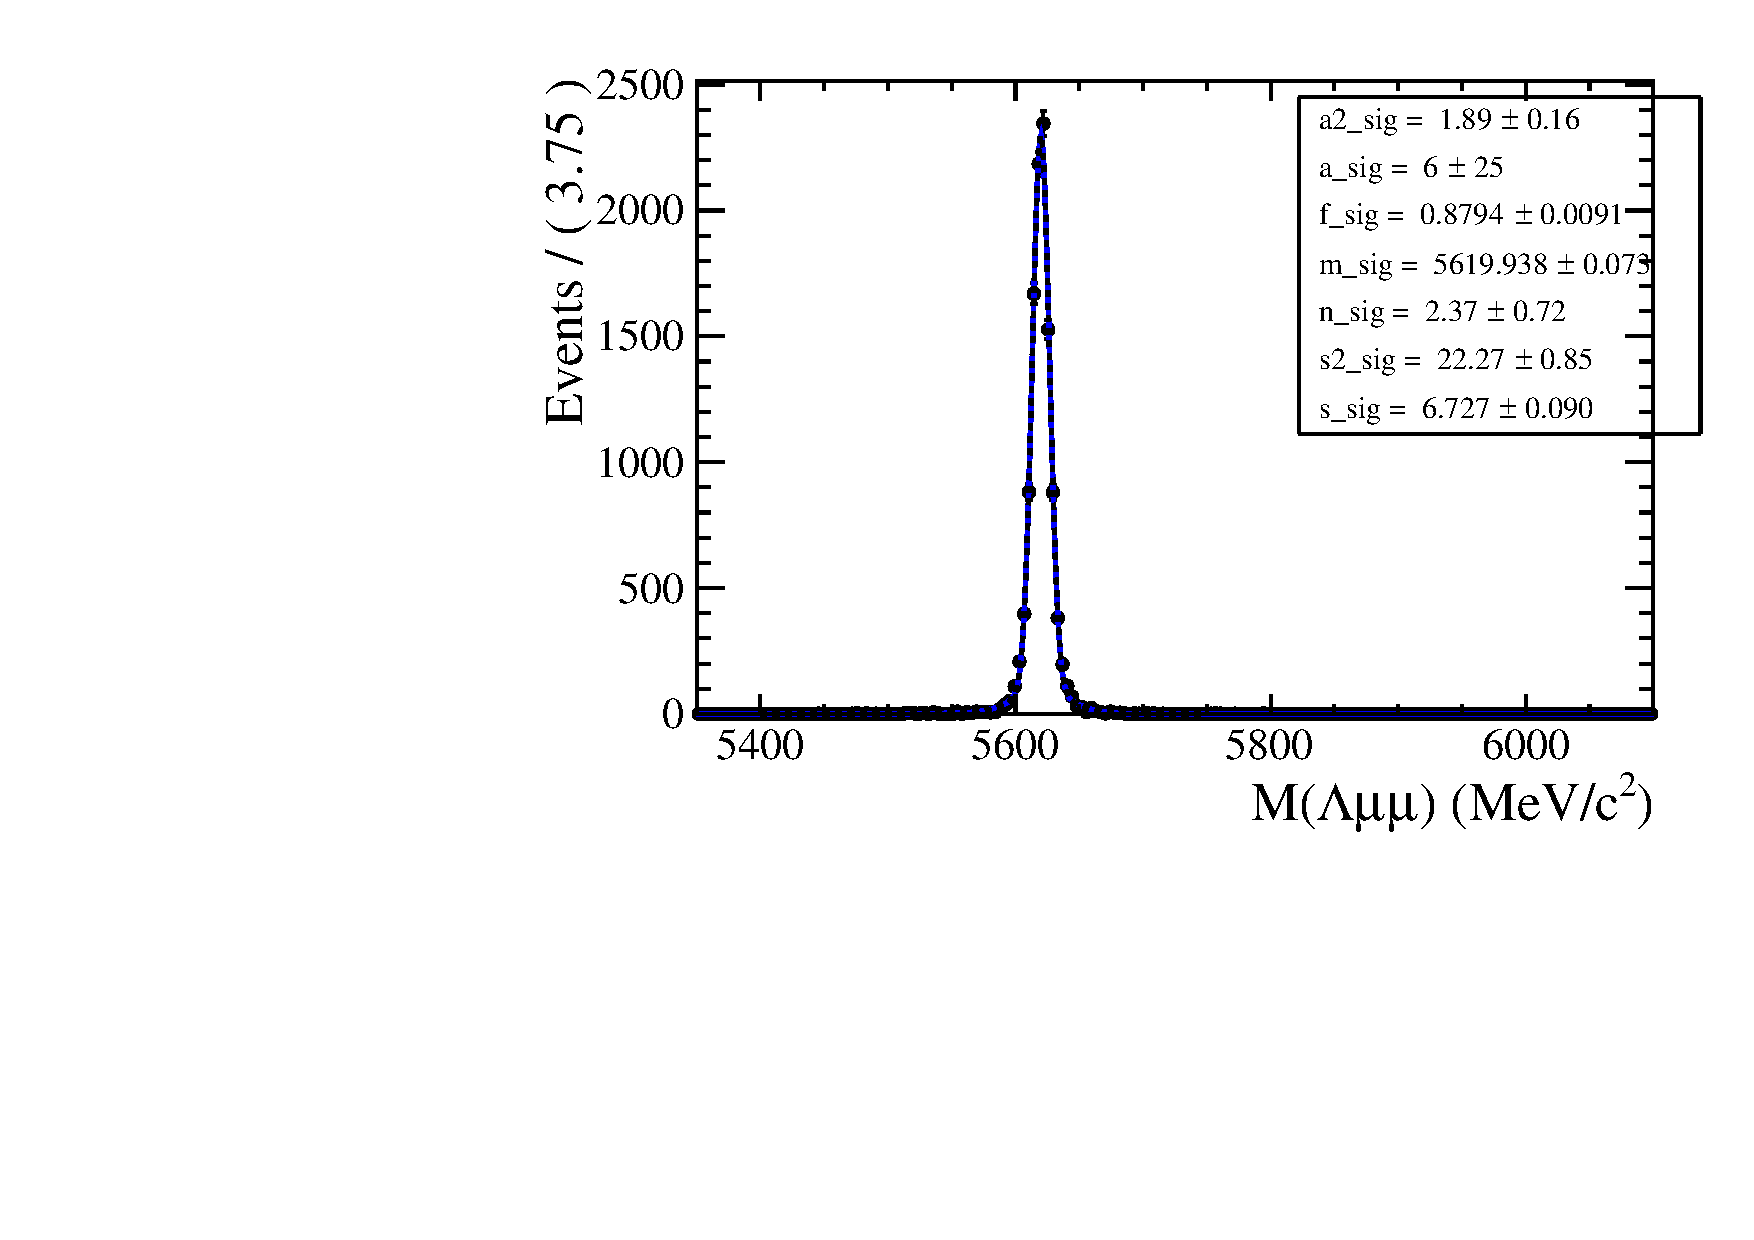
\includegraphics[width=0.49\textwidth]{Lmumu/figs/MassFits/fitLb2JpsiL_LL_MC.pdf}
\caption{Invariant mass distribution of $\Lb\ra\jpsi\Lz$ downstream (left) and long (right) candidates.
The points show simulated data and the blue line is the signal fit function.}
\label{fig:Lb_jpsiMCfit}
\end{figure}

In a second step the fit to the resonant channel data sample is performed.
For this fit the tail slope parameter, ``$n$", which is highly correlated
with $\alpha_1$ and $\alpha_2$, is fixed to the value found in the fit to simulated data.
In this fit two background components are modelled: the combinatorial background,
parameterized with an exponential and the background from $\Bz\ra\jpsi\KS$ decays.
The shape used to describe the \KS background is obtained from a $\Bz\ra\jpsi\KS$ simulated
sample to which the full selection is applied. The invariant distribution of these candidates
is fit with a DCB function, which is then used to model the \KS background
in the $\Lb\to\jpsi\Lz$ fit. The fit to the simulated $\Bz\ra\jpsi\KS$ events
is reported in Fig.~\ref{fig:KSbkgFit}. When the \KS shape is introduced in the fit to the data all
its parameters are fixed. This is particularly important when fitting long candidates, where the \KS
peak is less evident, which does not allow to constrain many parameters. On the other hand, in order
to take into account possible data-simulation differences, an horizontal shift is added and left
floating (by adding a constant to the central value of the DCB, $m_0 \ra m_0 + m'$).
In summary, the free parameters in the fit to the resonant $\Lb\to\jpsi\Lz$ sample
are the yields of the signal and the combinatorial and \KS backgrounds, the slope
of the exponential and the horizontal shift of the \KS shape. Note that all the parameters
of the PDFs used to fit the long and downstream samples are independent.

\begin{figure}
\centering
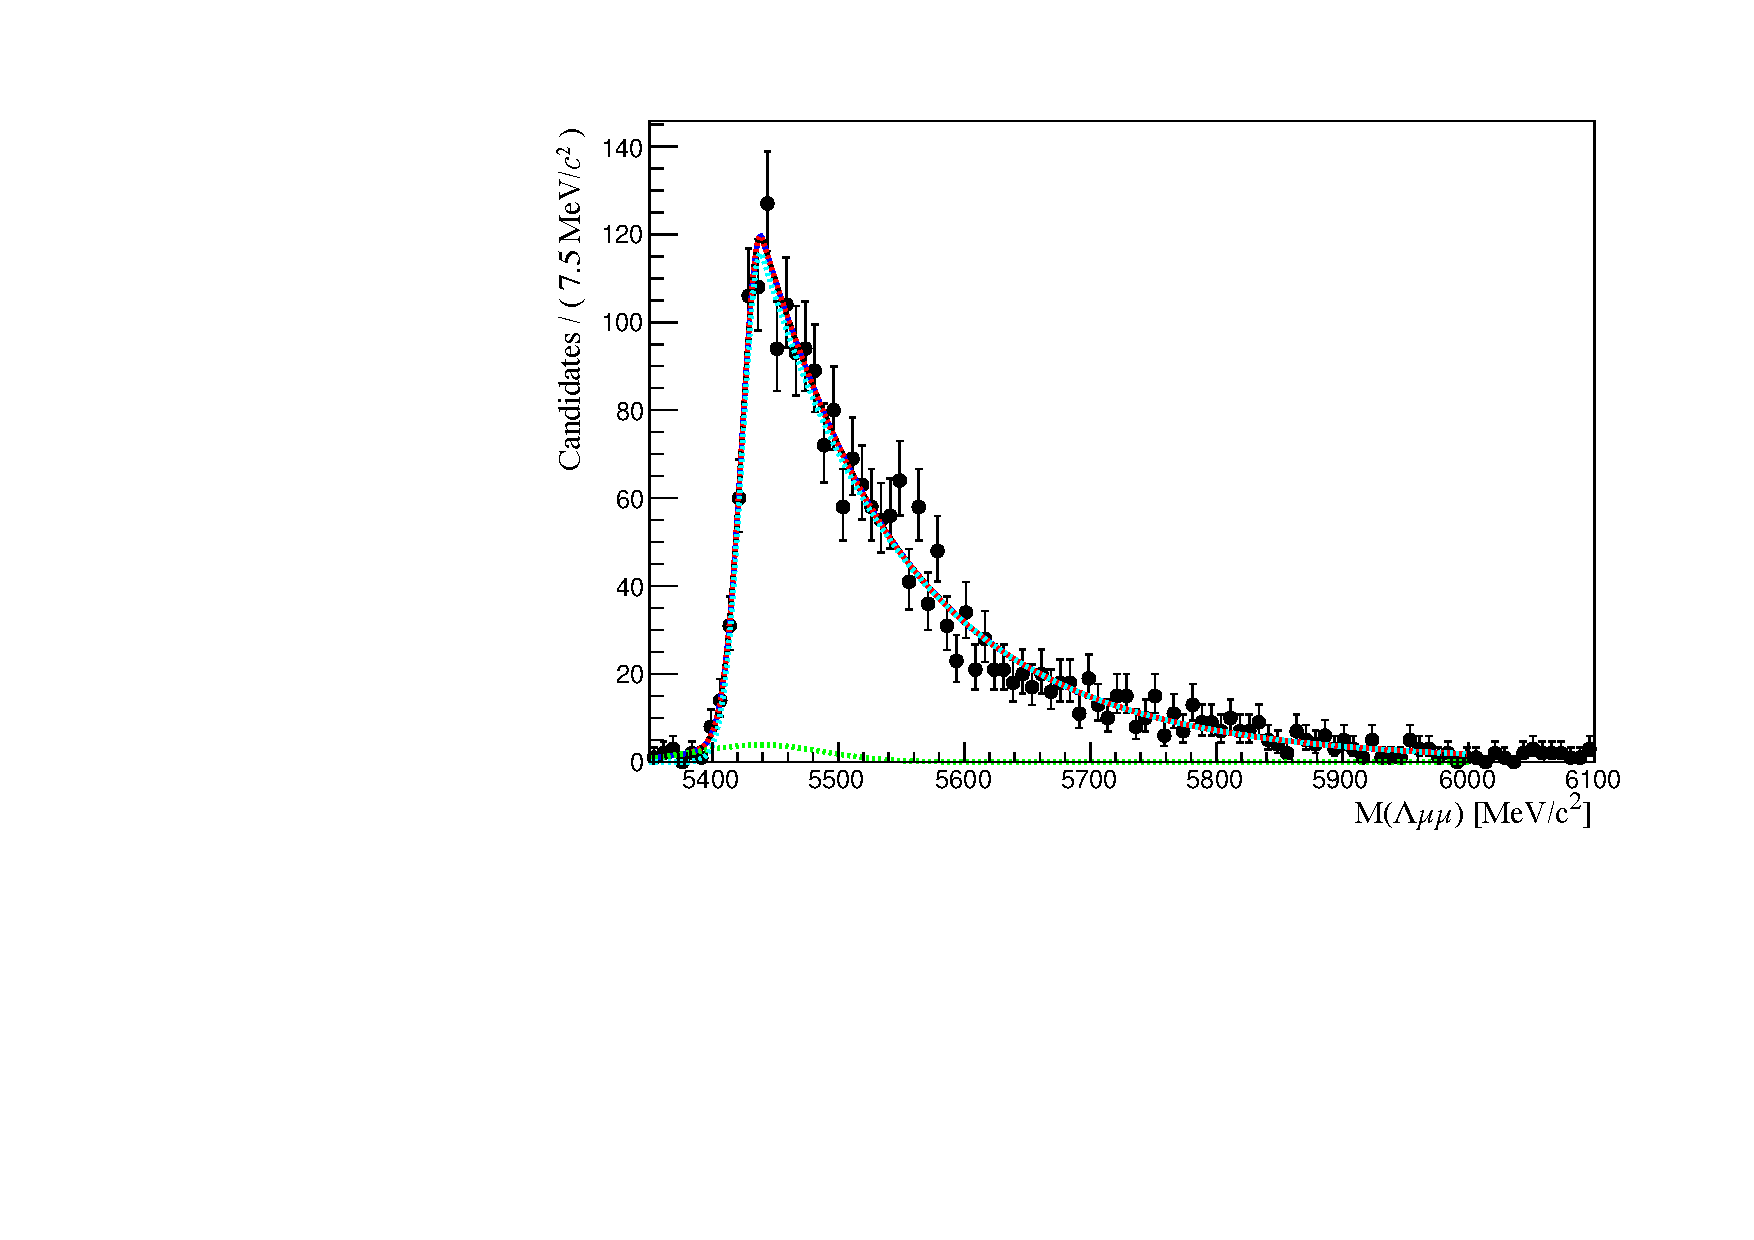
\includegraphics[width=0.6\textwidth]{Lmumu/figs/MassFits/fitKS_bkg.pdf}
\caption{Invariant mass distribution of simulated $\Bz\ra\jpsi\KS$ events after 
full selection fitted with a Double Crystal Ball function. }
\label{fig:KSbkgFit}
\end{figure}

Finally, the rare $\Lb\to\Lz\mumu$ data sample is fit. In this case the fit to the long
and downstream samples is performed simultaneously to obtain a more stable convergence. 
For this fit the signal is modelled with the same shape used in the resonant case as there is no physical
reason why they should be different. This method is also useful to limit systematic uncertainties
as the result will be given as a ratio between rare and resonant quantities.
However, the low statistics available in the rare sample does not allow to constrain many parameters.
%,especially when dividing data in \qsq bins.
Therefore, all parameters of the signal shape are fixed to
the ones derived from the fit to the $\jpsi\Lz$ channel. However, to account for possible differences, 
arising from a different resolution in different \qsq regions, a scale factor is multiplied
to the widths of the two gaussian cores of the signal DCB: $\sigma_1 \rightarrow c(\qsq)\cdot \sigma_1$
and $\sigma_2 \rightarrow c(\qsq)\cdot \sigma_2$, where the two scale factors are the same. These factors
are fixed to values obtained by fitting rare $\Lb\to\Lz\mumu$ simulated events in each \qsq bin and comparing
the widths with the ones found on the fit to the resonant simulated sample, namely
\begin{equation}
c = \sigma_{\mumu}^{MC} / \sigma_{\jpsi}^{MC}.
\end{equation}
These values are found to be $\sim 1.9$ for downstream candidates and $\sim 2.3$ for long candidates,
corresponding to the fact that in the resonant case a further constrain on the dimuon mass
is used, which improves the resolution by a factor of $\sim2$. The dependence of the scaling factor on \qsq 
is found to be small. For the fits on the long and downstream samples the parameters are always separately fixed to the
corresponding $\jpsi\Lz$ fits; in this analysis shape parameters are never shared between the two candidate categories.

The modelled background components are, also in the rare case,
the combinatorial background, described with an exponential function and the \KS background. 
The slope of the background is visibly different depending on the \qsq interval. This is partly due to the 
fact that at high \qsq the combinatorial changes slope because of a kinematical limit at low 4-body
masses imposed by the \qsq requirements. The exponential slopes are therefore left as independent
parameters in each \qsq interval. % and for the downstream and long samples.
The background component from $\Bz\to\KS\mumu$ decays is modelled using the same shapes used
for the resonant channel. However, in this case the horizontal shift is fixed to what found
for the resonant channel. The expected amount of misreconstructed $\Bz\ra\KS\mumu$
candidates is small and does not allow to determine reliably its yield. Therefore, 
this is fixed to the yield of $\Bz\ra\jpsi\KS$ decays rescaled by the expected ratio
of branching fractions between the resonant and rare channels. The \qsq distribution of $\Bz\ra\KS\mumu$ 
simulated events is used to predict the yield as a function of \qsq. Table~\ref{tab:KSprediction} reports the 
number of predicted $\Bz\ra\KS\mumu$ candidates in each \qsq interval obtained with the following formula:
\begin{equation}
N_{\KS\mumu}(\qsq) = N_{\jpsi\KS}\frac{B(\Bz\ra\KS\mumu)}{B(\Bz\ra\KS\jpsi)}\cdot \frac{1}{\varepsilon_{rel}} \cdot B(\jpsi\ra\mumu) \frac{N(\qsq)_{MC}}{N^{tot}_{MC}} 
\end{equation}
where $N(\qsq)_{MC}$ is the number of simulated rare candidates falling in a \qsq interval after full selection and $N^{tot}_{MC}$ 
is the total number of simulated events and \mbox{$\varepsilon_{rel} = \varepsilon_{\mu\mu} / \varepsilon_{\jpsi}$} is the relative selection efficiency between the two channels. 
%The \KS\mumu contribution is then completely taken out to study systematic
%uncertainties as described in Sec.~\ref{sec:Lb_sys}.
%Only for the 6-8 \gevgevcccc bin, a background component coming from the residual of the \jpsi radiative tail is
%added, modelled using a the shape obtained studying simulated events and smoothed using the \verb!RooKeysPdf! method of \verb!RooFit!.
%This is then removed from the final fit becuase it returns zero yield.

\begin{table}
\centering
\caption{Predicted numbers of $\Bz\ra\KS\mumu$ events in each considered \qsq interval.}
\begin{tabular}{$l^c^c}
	\rowstyle{\bfseries}
 \qsq interval [\gevgevcccc]  & Downstream & Long \\ \hline
0.1--2.0 & 0.9 & 0.1 \\
2.0--4.0 & 0.9 & 0.1 \\
4.0--6.0 & 0.8 & 0.1 \\
6.0--8.0 & 1.1 & 0.1 \\
11.0--12.5 & 1.9 & 0.2 \\
15.0--16.0 & 1.1 & 0.1 \\
16.0--18.0 & 2.0 & 0.2 \\
18.0--20.0 & 1.1 & 0.1 \\ \hline
1.1--6.0 & 2.1 & 0.1 \\
15.0--20.0 & 4.2 & 0.5 \\ 
\end{tabular}
\label{tab:KSprediction}
\end{table}

As the fit to the rare sample is performed simultaneously on long and downstream candidates,
their two yields are not free to vary separately but are parameterised
as a function of the common branching fraction using the following formula:
%
\begin{equation}
N(\Lz\mumu)_{k}  = \left[ \frac{\mathrm{d}\mathcal{B}(\Lz\mumu)/\mathrm{d}\qsq}{\mathcal{B}(\jpsi\Lz)} \right]  \cdot
N(\jpsi\Lz)_{k} \cdot \varepsilon^{\mathrm{rel}}_{k} \cdot \frac {\Delta\qsq} { \mathcal{B}(\jpsi\to\mumu) },
\label{eq:relYield}
\end{equation}
%
where $k = $(LL,DD), $\Delta\qsq$ is the width of the \qsq interval and the only free parameter is the relative branching 
fraction ratio of the rare over \jpsi channels. For the branching fraction of the \jpsi\to\mumu decay the value 
reported in the PDG book, \mbox{$(5.93 \pm 0.06)\cdot 10^{-2}$~\cite{PDG2014}} is used and $\varepsilon^{rel}$ corresponds to
the relative efficiency between the rare and resonant channels obtained in Sec.~\ref{sec:Lb_eff}. 
In this formula the efficiencies and the normalisation yield appear as constants, namely 
$N(\Lz\mumu)_{k} = C_k \cdot \mathcal{B}^{rel}$. 
%These constants are then varied in order to obtain 
%systematic uncertainties on the final result as described in Sec.~\ref{sec:Lb_sys}.


\subsection{Fit results}



\begin{figure}
\centering
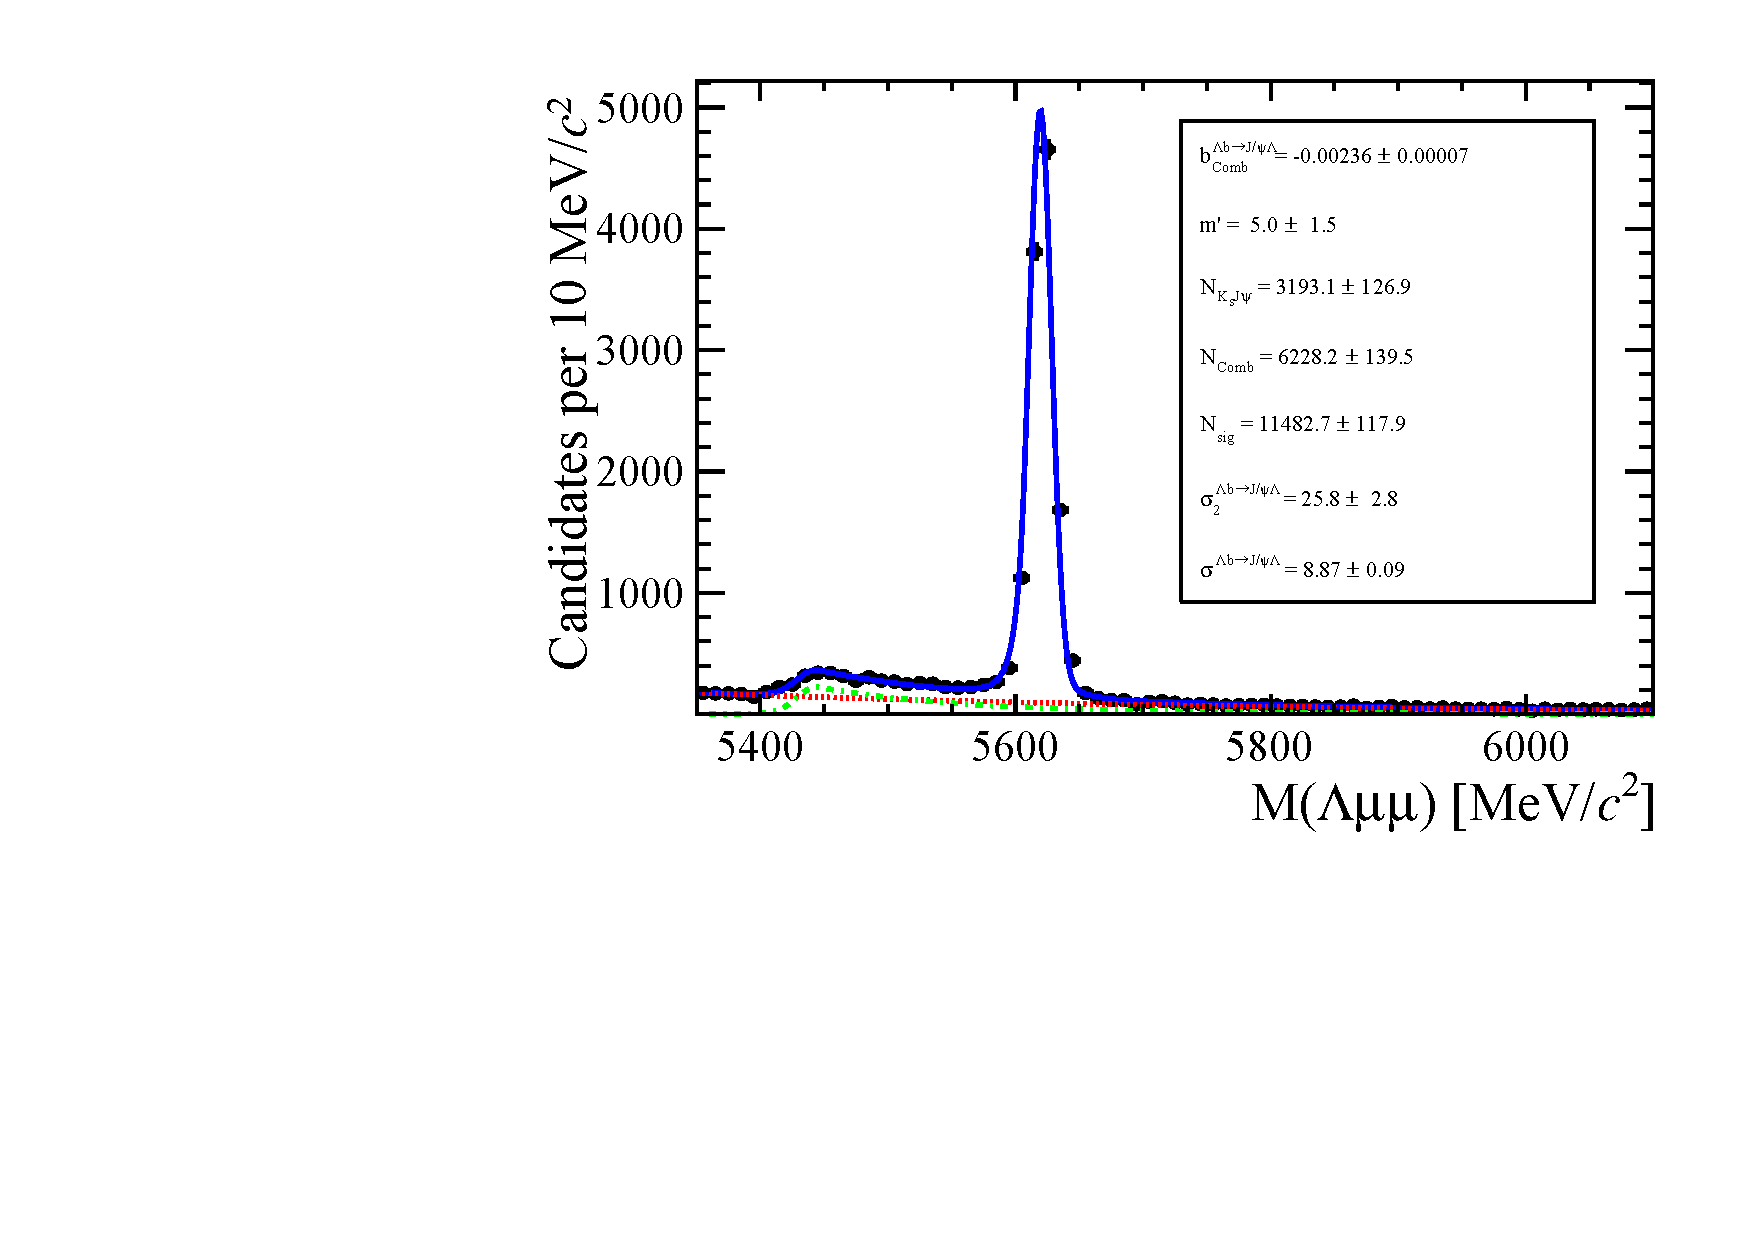
\includegraphics[width=0.75\textwidth]{Lmumu/figs/MassFits/Lb2JpsiL__DD_data.pdf}
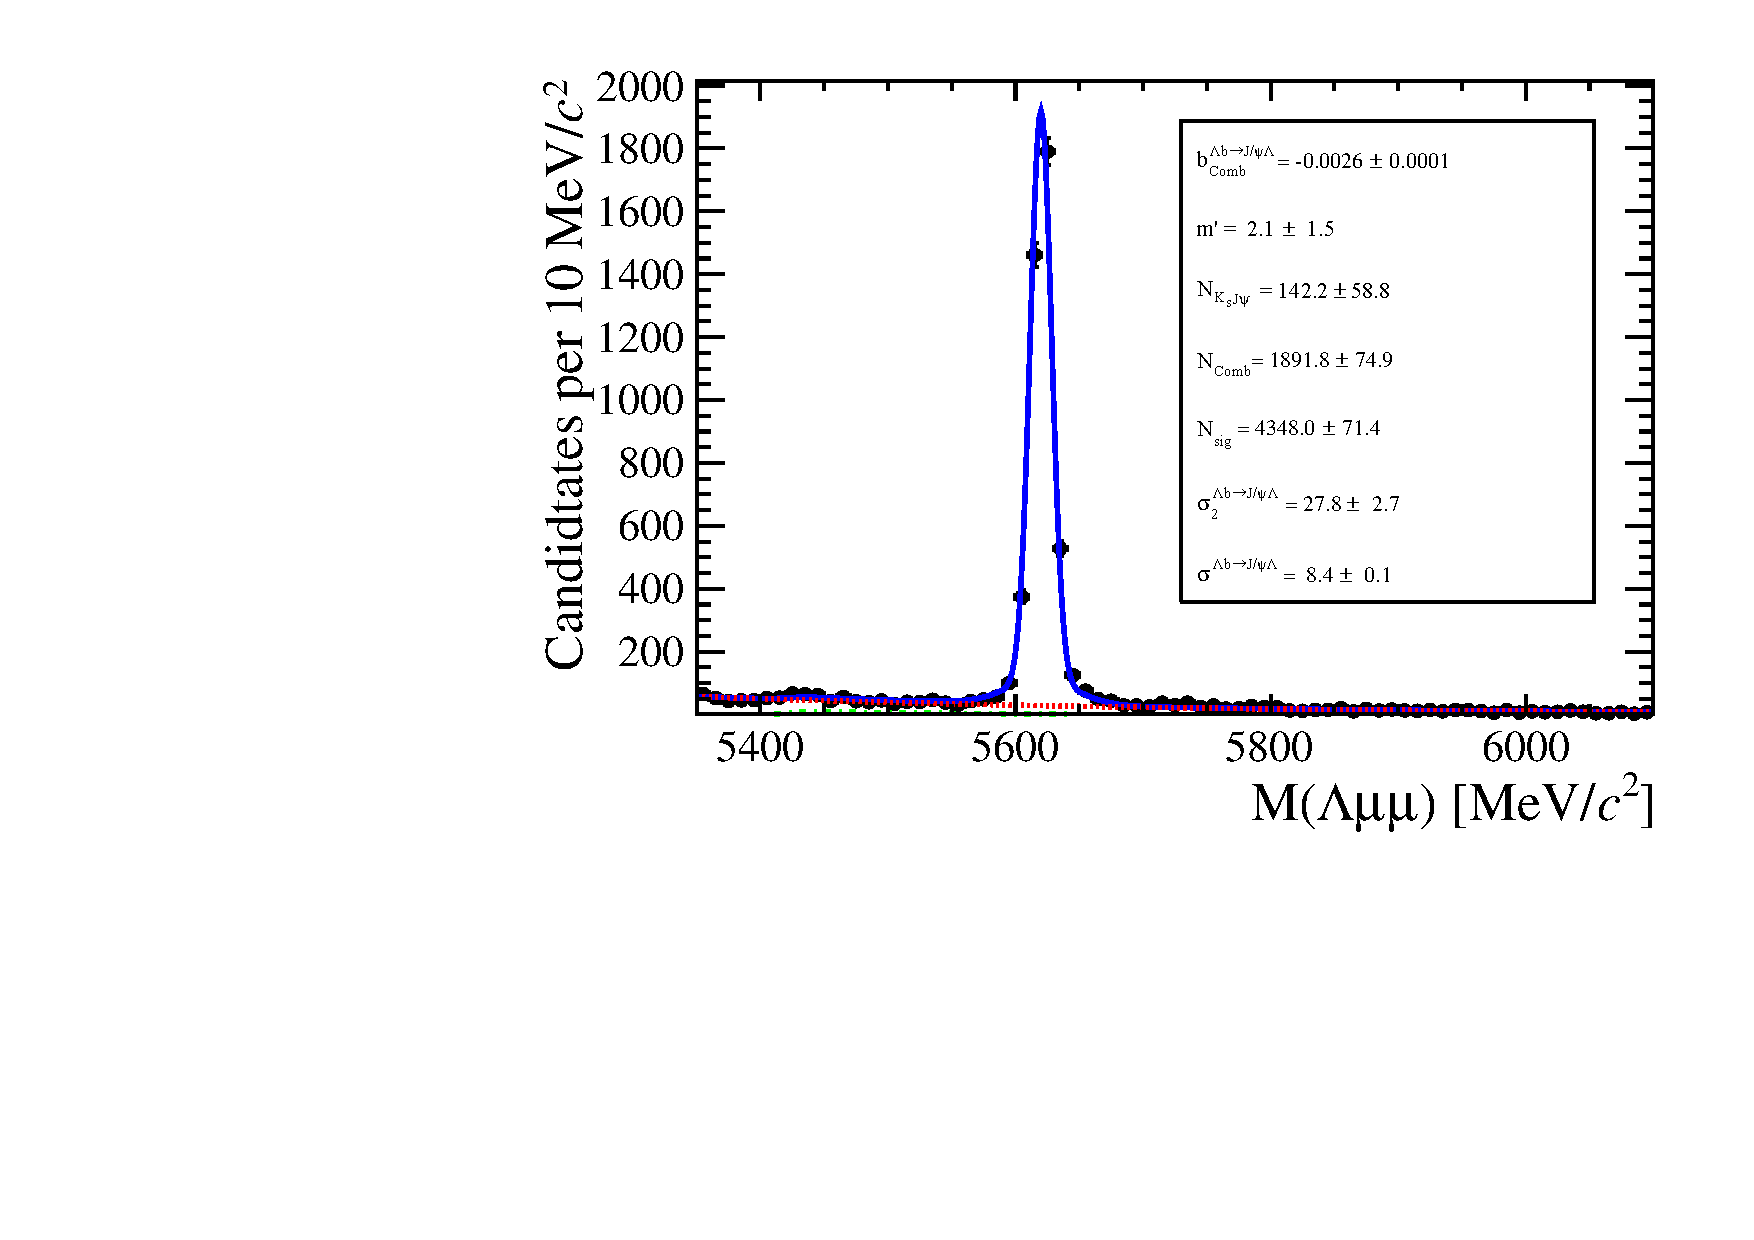
\includegraphics[width=0.75\textwidth]{Lmumu/figs/MassFits/Lb2JpsiL__LL_data.pdf}
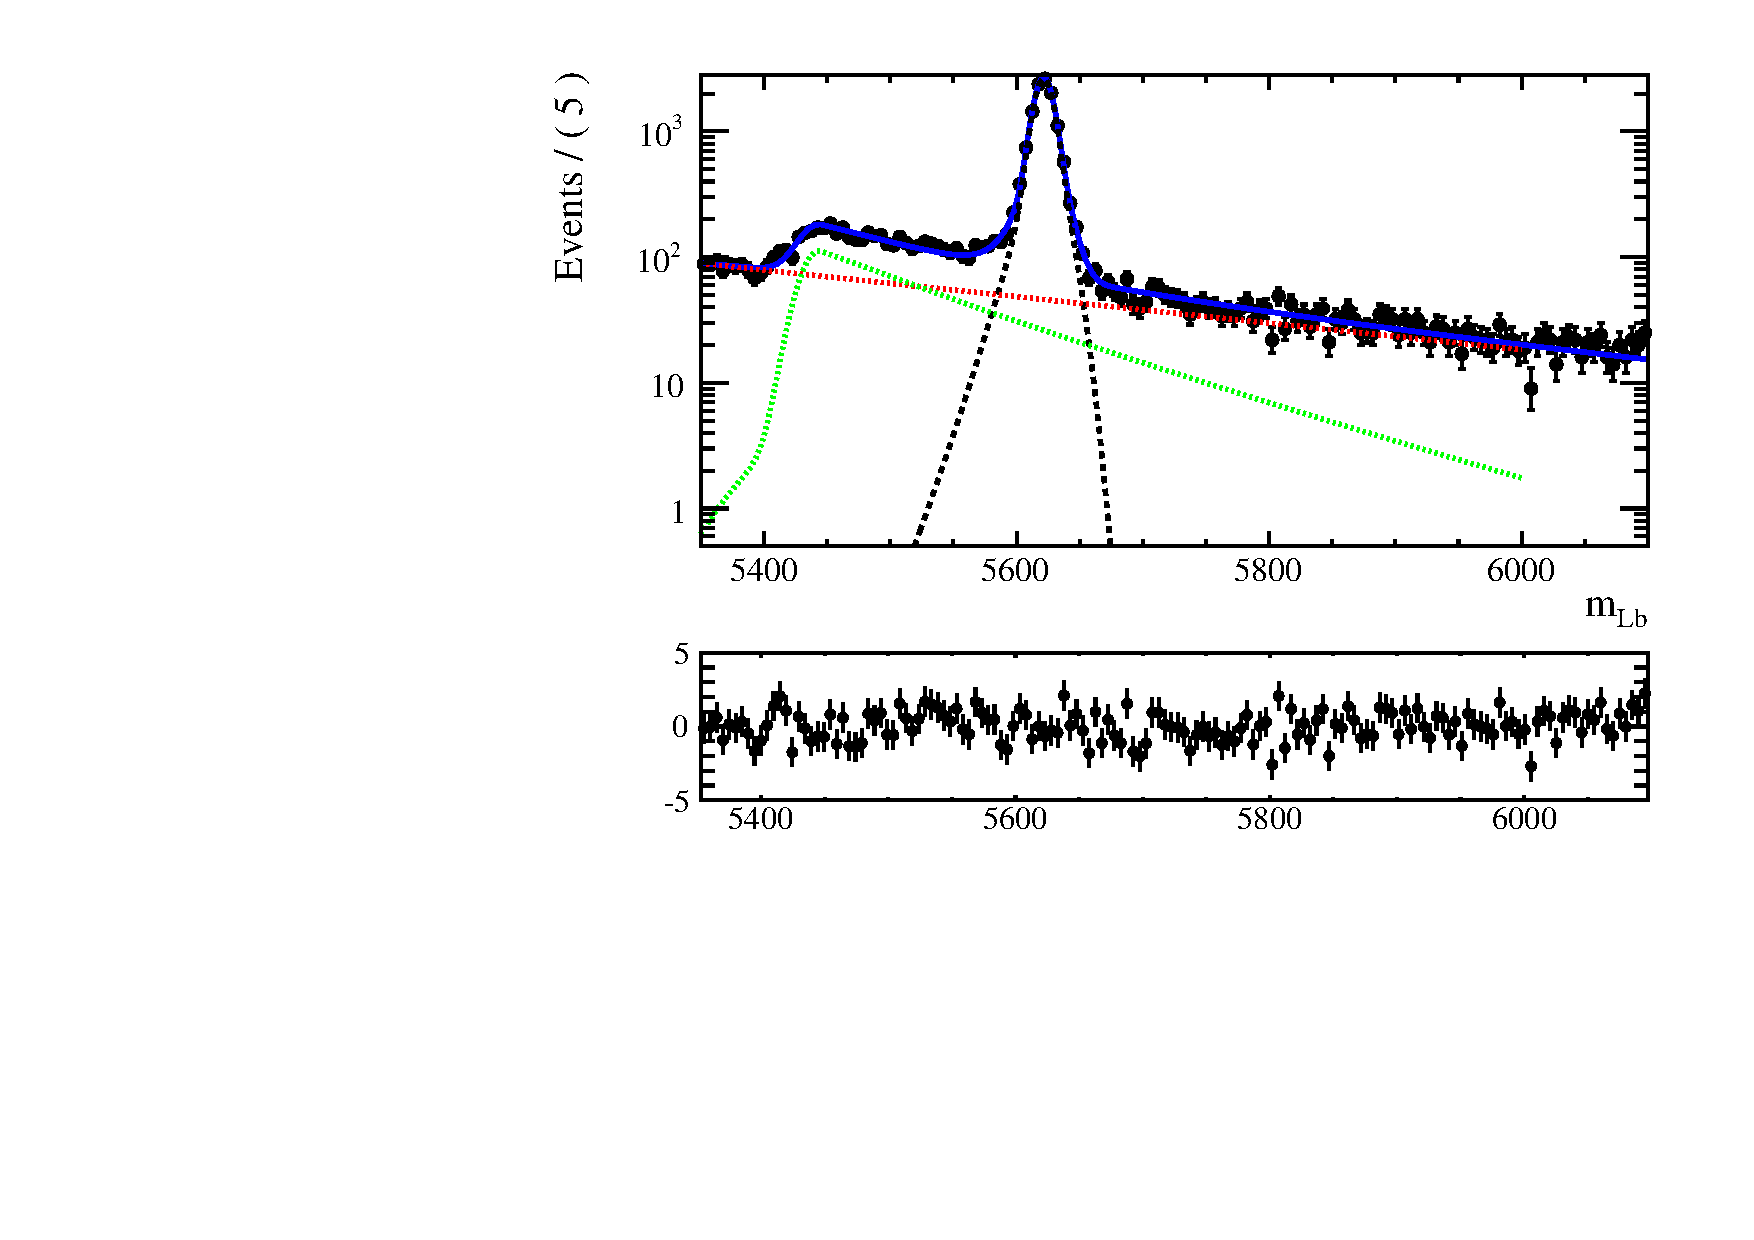
\includegraphics[width=0.49\textwidth]{Lmumu/figs/MassFits/Lb2JpsiL_DD_data_log_fitAndRes.pdf}
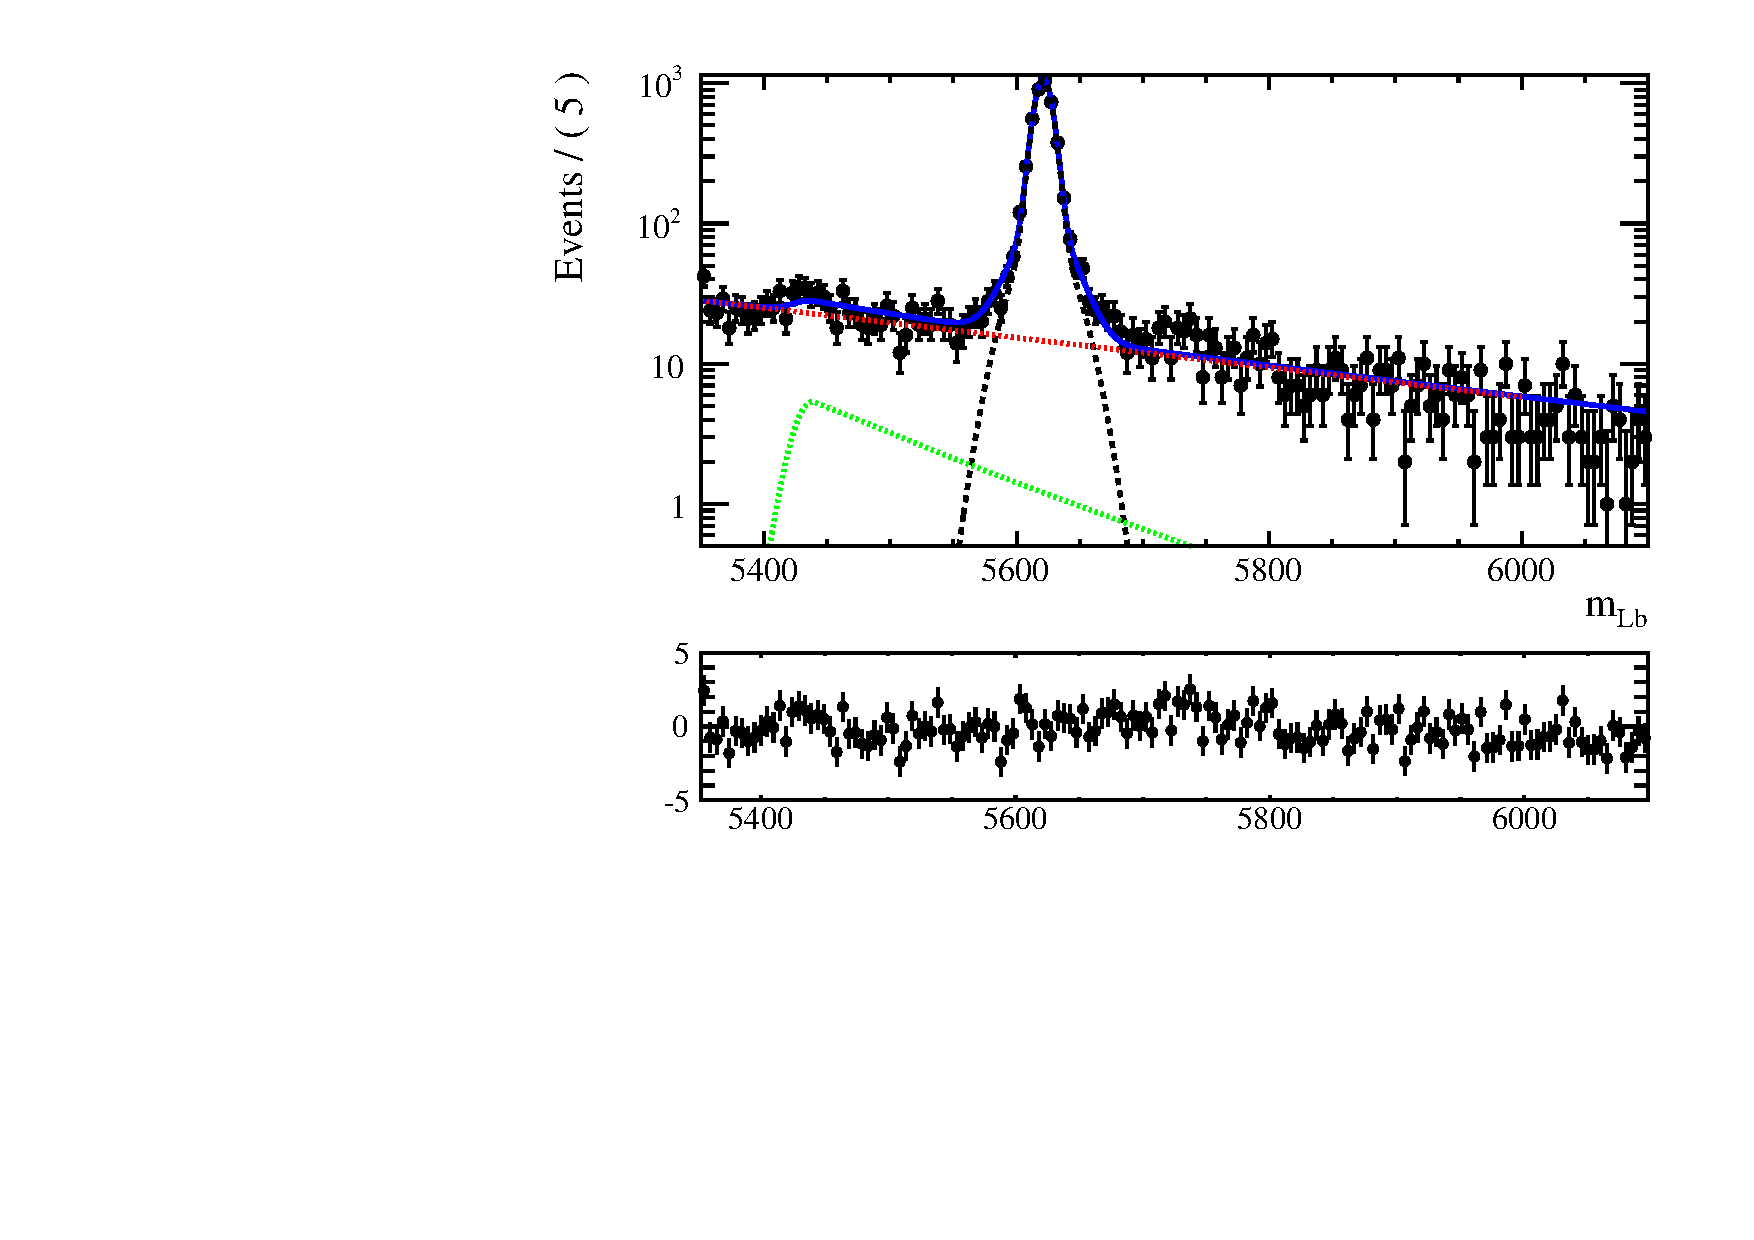
\includegraphics[width=0.49\textwidth]{Lmumu/figs/MassFits/Lb2JpsiL_LL_data_log_fitAndRes.pdf}
\caption{Invariant mass distributions of $\Lb\ra\jpsi\Lz$ downstream (top) and long (middle) candidates
selected with high \qsq requirements.
Bottom plots are the same as the upper ones but shown in logarithmic scale. Black points show data.
The blue solid line represents the total fit function, the black dashed line the signal, the red dashed line
the combinatorial background and the green dashed line the $\Bz\ra\KS\mumu$ background.}
\label{fig:Lb_totalFit}
\end{figure}
%
Figures~\ref{fig:Lb_totalFit} and~\ref{fig:Lb_totalFit_low} show fitted invariant mass distributions for
the normalisation channel, selected with the high-\qsq and low-\qsq requirements respectively.
%The $\chi^2$ value of the fit is $126$ for LL and $112$ for DD both with 140 degrees of freedom, which corresponds to probability of 80\% and 95\%.
Table~\ref{tab:Lb_rawYieldJpsi} reports the measured yields of $\Lb\ra\jpsi\Lz$ candidates found using the low- 
and \mbox{high-\qsq} selections. Values for the signal shape parameters are shown on Fig.~\ref{fig:Lb_totalFit}.
Fits to the rare $\Lb\ra\Lz\mumu$ samples are shown in Fig.~\ref{fig:Lb_Lmumu} for the integrated
$15 < \qsq < 20$ and $1.1 < \qsq < 6.0$~\gevgevcccc ~\qsq intervals, while
%The exponential slopes, the scale factors multiplied to the widths and the number of combinatorial events
%found from these fits are reported in Tab.~\ref{tab:Lb_rareParam}.
fitted invariant mass distribution in all other considered \qsq intervals are in Figs.~\ref{fig:Lb_differentialFitDD}
and~\ref{fig:Lb_differentialFitLL} for downstream and long candidates respectively.
The yields of rare candidates obtained from the fit are listed in Tab.~\ref{tab:Lb_rawYield} together with their significances.
Most candidates are found in the downstream sample, which comprises $\sim 80\,\%$ of the total yield.
Note that, since the fit is simultaneous to the two candidate categories, their yields
are not parameters free to vary independently but are correlated via the branching ratio.
The statistical significance of the observed signal yields is evaluated as the change in the logarithm 
of the likelihood function, $\sqrt{2\Delta\ln{\mathcal{L}}}$, when the signal component
is excluded from the fit, relative to the nominal fit in which it is present.

\begin{table}
\centering
\caption{Number of \decay{\Lb}{\jpsi\Lz} candidates in the downstream and
  long categories found using the for low- and
  high-\qsq requirements; uncertainties are statistical only.}
\begin{tabular}{$l^c^c}
\rowstyle{\bfseries}
Selection & Long & Downstream					\\ \hline
high-\qsq	& $4313 \pm 70$	 	&  $11\,497 \pm 123$ \\
low-\qsq	& $3363 \pm 59$ 	&  $\phantom{0}\,7225 \pm 89\phantom{0}$  \\
 \hline
\end{tabular}
\label{tab:Lb_rawYieldJpsi}
\end{table}

\begin{table}
\centering
\caption{Signal yields, $N_\mathrm{S}$, obtained from the
  invariant mass fit to \decay{\Lb}{\Lz\mumu} candidates in each \qsq interval
  together with their statistical significance. 
  The \mbox{$8-11$} and \mbox{$12.5-15$}~\gevgevcccc ~\qsq intervals are excluded
  from the study as they are dominated by resonant decays via charmonium resonances.}
\begin{tabular}{$l^c^c^c^c}
\rowstyle{\bfseries} 
 \qsq interval [\gevgevcccc] & DD & LL & Tot. yield & Significance \\ \hline
\phantom{x}0.1 -- 2.0\phantom{x}   &  $\phantom{x}6.9 \pm 2.2$  &  $\phantom{xx}9.1 \pm 3.0\phantom{x}$	 &  $16.0\pm5.3$            		&  4.4 \\
\phantom{x}2.0 -- 4.0\phantom{x}   &  $\phantom{x}1.8 \pm 1.7$  &  $\phantom{xx}3.0 \pm 2.8\phantom{x}$ 	 &  $\phantom{x}4.8\pm4.7$  	 &  1.2 \\
\phantom{x}4.0 -- 6.0\phantom{x}   &  $\phantom{x}0.4 \pm 0.9$  &  $\phantom{xx}0.6 \pm 1.4\phantom{x}$	 &  $\phantom{x}0.9\pm2.3$  	 &  0.5 \\
\phantom{x}6.0 -- 8.0\phantom{x}   &  $\phantom{x}4.3 \pm 2.0$   &  $\phantom{xx}7.2 \pm 3.3\phantom{x}$	 &  $11.4\pm5.3$            		&  2.7 \\
11.0 -- 12.5  				     &  $14.6 \pm 2.9$  		    &  $\phantom{x}42.8 \pm 8.5\phantom{x}$  &  $\phantom{x.}60\pm12\phantom{.}$ &  6.5 \\
15.0 -- 16.0  			             &  $13.5 \pm 2.2$  		    &  $\phantom{x}43.5 \pm 7.2\phantom{x}$   &  $\phantom{x.}57\pm9\phantom{x.}$             			 &  8.7 \\
16.0 -- 18.0  				    &  $28.6 \pm 3.3$  		    &  $\phantom{x}88.8 \pm 10.1$	 	       &  $\phantom{.}118\pm13\phantom{.}$              			 &  13  \\
18.0 -- 20.0  				    &  $22.4 \pm 2.6$  		    &  $\phantom{x}78.0 \pm 8.9\phantom{x}$ &  $\phantom{.}100\pm11\phantom{.}$    &  14  \\
\hline
\phantom{x}1.1 -- 6.0\phantom{x}    	&  $\phantom{x}3.6 \pm 2.4$  &  $\phantom{xx}5.7 \pm 3.8\phantom{x}$	 &  $\phantom{x}9.4\pm6.3$  			&  1.7 \\
15.0 -- 20.0  					&  $64.6 \pm 4.7$  			&  $209.6 \pm 15.3$ 					&  $\phantom{.}276\pm20\phantom{.}$              		&  21  \\
\end{tabular}
\label{tab:Lb_rawYield}
\end{table}

\begin{figure}
\centering
\includegraphics[width=0.49\textwidth]{Lmumu/figs/MassFits/Lb2JpsiL__lowSel_DD_data.pdf}
\includegraphics[width=0.49\textwidth]{Lmumu/figs/MassFits/Lb2JpsiL__lowSel_LL_data.pdf}
\caption{Invariant mass distribution of $\Lb\ra\jpsi\Lz$ for downstream (left) and long (right) candidates
 selected with low \qsq requirements.}
\label{fig:Lb_totalFit_low}
\end{figure}
%
%
\begin{figure}
\centering
\includegraphics[width=0.7\textwidth]{Lmumu/figs/paper/figure13.pdf}
\includegraphics[width=0.7\textwidth]{Lmumu/figs/paper/figure2.pdf}
\caption{Invariant mass distributions of $\Lb\ra\Lz\mumu$ candidates in the integrated $0.1 - 6.0$ (top)
and $15 - 20$~\gevgevcccc (bottom) ~\qsq intervals. Points show data combining long and downstream candidates together.
The blue solid line represents the total fit function and the dashed red line the combinatorial background.}
%\includegraphics[width=0.54\textwidth]{Lmumu/figs/MassFits/Lb2Lmumu_DD_lowQ2_fitAndRes.pdf}
%\includegraphics[width=0.54\textwidth]{Lmumu/figs/MassFits/Lb2Lmumu_LL_lowQ2_fitAndRes.pdf}
%\includegraphics[width=0.54\textwidth]{Lmumu/figs/MassFits/Lb2Lmumu_DD_highQ2_fitAndRes.pdf}
%\includegraphics[width=0.54\textwidth]{Lmumu/figs/MassFits/Lb2Lmumu_LL_highQ2_fitAndRes.pdf}
%\caption{Invariant mass distribution of $\Lb\ra\Lz\mumu$ candidates in the integrated 0.1--6.0 (top)
%\gevgevcccc ~\qsq interval for downstream (left) and long (right) candidates. The points show data, the blue line
%and 15.0--20.0 (bottom) \gevgevcccc \qsq intervals.
%The blue solid line represents the total fit function and the dashed red line the combinatorial background.}
\label{fig:Lb_Lmumu}
\end{figure}
%
\begin{figure}
\centering
\includegraphics[width=1.\textwidth]{Lmumu/figs/MassFits/q2_fits_DD_plot2.pdf}
\includegraphics[width=1.\textwidth]{Lmumu/figs/MassFits/q2_fits_DD_plot1.pdf}
\caption{Invariant mass distributions of rare $\Lb\ra\Lz\mumu$ downstream candidates in the considered \qsq intervals.
 %[0.1,2], [2,4], [4,6], [6,8], [11,12.5], [15,16], [16,18], [18,20] 
 }
\label{fig:Lb_differentialFitDD}
\end{figure}

\begin{figure}
\centering
\includegraphics[width=1.\textwidth]{Lmumu/figs/MassFits/q2_fits_LL_plot2.pdf}
\includegraphics[width=1.\textwidth]{Lmumu/figs/MassFits/q2_fits_LL_plot1.pdf}
\caption{Invariant mass distributions of rare $\Lb\ra\Lz\mumu$ long candidates in the considered \qsq intervals.
 %[0.1,2], [2,4], [4,6], [6,8], [11,12.5], [15,16], [16,18], [18,20] 
 }
\label{fig:Lb_differentialFitLL}
\end{figure}



%\begin{table}
%\centering
%\caption{Values of exponential slope, $b$, and scale factors, $c$ found from the fit
%to the resonant data sample and fixed from the fit to the rare data sample.}
%\begin{tabular}{|c|c|c|}
%\hline
%Parameter  			 & Downstream & Long	\\ 
%\hline
%\multicolumn{3}{|c|}{ 15.0--20.0 \gevgevcccc}  \\
%\hline

%$b$ 				& $0.0006 \pm 0.0003$		 		& 	$0.0012 \pm 0.0008$        \\
%$c$ 				& $1.9027 \pm 0.0001$ 				&	$2.2910 \pm 0.0001$        \\
%%$N_{exp}$ 			& $393^{+23}_{-22}$	&	 $64^{+9}_{-8}$       \\

%\hline
%\multicolumn{3}{|c|}{ 1.1--6.0 \gevgevcccc}  \\

%\hline
%$b$ 				& $-0.0026 \pm 0.0004$				&	$-0.0036 \pm 0.0011$	 \\
%$c$ 				& $1.9208 \pm 0.0001$				&	$2.3504 \pm 0.0001$        \\
%%$N_{exp}$ 			& $203^{+15}_{-14}$	&	$34^{+7}_{-6}$       \\
%\hline

%\end{tabular}
%\label{tab:Lb_rareParam}
%\end{table}




\clearpage


\chapter{Efficiency}
\label{sec:Lb_eff}

The efficiency for each of the decays is calculated according to the formula
\begin{equation}
\varepsilon^{tot}=\varepsilon(Geom)\varepsilon(Det|Geom)\varepsilon(Reco|Det)\epsilon(MVA|Reco)\varepsilon(Trig|MVA).
\end{equation}
In this expression the first term gives the efficiency to have final state particles in the LHCb acceptance.
The second term handles the possibility of \Lz escaping the detector or interacting with it and therefore
never decaying into $p\pi$. This term is referred to as ``detection" efficiency.
The third term carries information about the reconstruction and pre-selection efficiencies,
which are kept together given that boundaries between them are completely artificial.
The fourth part deals with the efficiency of the Neural Network for those events which passed the pre--selection. 
Finally, the last term handles the trigger efficiency.
%Trigger efficiency is calculated before the MVA one because the training is performed on untriggered data to save statistics.
Most of the efficiency components are evaluated using the simulated samples described in Sec.~\ref{sec:Lb_simulation}.
Only the efficiency of PID requirement for the proton (see Tab.~\ref{tab:Lb_stripping}) is separately derived
with a data--driven method because the simulation does not provide a good description of PID variables.
For complete information, all absolute efficiencies for the two decays $\Lb\to\Lz\mumu$ and $\Lb\to\jpsi\Lz$ are
separately listed in the next sections. However, for the analysis itself only relative efficiency,
$\varepsilon($\Lb\to\Lz\mumu$)/\varepsilon(\Lb\to\jpsi\Lz)$, is used. 


\section{Geometric acceptance}
\label{sec:Lb_geomAcc}
In order to save disk space and time, only events are simulated, in which the final muons
are in the detector acceptance and therefore can be reconstructed. This corresponds to a requirement for each
of the muons to be in an interval \mbox{$10 < \theta < 400$~mrad}, where $\theta$ is the angle between
the muon momentum and the beam line. The efficiency of this requirement is obtained by using 
a separate simulated sample, where events are generated in the full space.
In Tab.~\ref{tab:Lb_geom_eff} the efficiencies due to the geometrical acceptance are listed
in bins of \qsq for $\Lb\to\Lz\mumu$ decays.
%
\begin{table}[h]
\centering
\caption{Absolute geometrical acceptance in bins of \qsq derived from generator level 
simulated samples. Uncertainties are statistical only.}
\begin{tabular}{lc}\hline
\qsq [\gevgevcccc]     & Geom. acc.   \\ \hline
0.1--2.0 		&  $0.2359 \pm 0.0008$  \\
2.0--4.0 		&  $0.2098 \pm 0.0007$  \\
4.0--6.0 		&  $0.2008 \pm 0.0007$  \\
6.0--8.0 		&  $0.1960 \pm 0.0008$  \\
%9.1--10.1 	&  $0.1927 \pm 0.0012$  \\
11.0--12.5 	&  $0.1897 \pm 0.0010$  \\
15.0--16.0 	&  $0.1896 \pm 0.0015$  \\
16.0--18.0 	&  $0.1872 \pm 0.0012$  \\
18.0--20.0 	&  $0.1870 \pm 0.0016$  \\
\hline
1.1--6.0 	&  $0.2072 \pm 0.0005$  \\
15.0--20.0 	&  $0.1876 \pm 0.0008$  \\
\hline
\end{tabular}
\label{tab:Lb_geom_eff}
\end{table}


\section{Reconstruction and neural network efficiencies}

The efficiency to reconstruct the decays together with the pre-selection requirements is
evaluated from simulated data. 
%For the evaluation we use the most recent LHCb measurement of \Lb
%lifetime of $1.482\pm0.03$ ps\cite{LHCb--PAPER--2013--032} and \Lb polarisation $0.06\pm0.09$ \cite{Aaij:2013oxa}.
Table~\ref{tab:Lb_recoEff} reports values of reconstruction efficiency in bins of \qsq for long and downstream candidates.
In the table the efficiency is subdivided in ``Detection" and ``Reconstruction and pre-selection" efficiencies.
In fact, since \Lz is a long lived particle, there is a non-negligible probability that it interacts in the detector
or escapes from it and therefore never decays in proton and pion. The efficiency for this to happen is what
is called ``Detection" efficiency. The ``Reconstruction and Stripping" efficiency includes the efficiency of
for the tracks to produce observable signatures and the efficiency for candidates to pass the pre-selection 
requirements. This component does not include the efficiency
of the PID cut that appears in Tab.~\ref{tab:Lb_stripping}, which is kept separate
because PID variables are not well described by the simulation and therefore a
data-driven method is used instead (see Sec.~\ref{sec:PIDeff}).

%
\begin{table}[h]
\centering
\caption{Absolute detection and reconstruction plus stripping efficiencies.
Reconstruction efficiency is given separately for DD and LL candidates. Uncertainties are statistical only. }
\begin{tabular}{lccc}\hline
\qsq [\gevgevcccc] & Detection & Reco and pre-sel (DD) & Reco and pre-sel (LL) \\ \hline
0.1--2.0 		&  $0.8793 \pm 0.0005$	&  $0.0519 \pm 0.0006$	&  $0.0194 \pm 0.0004$  \\
2.0--4.0 		&  $0.8850 \pm 0.0004$	&  $0.0664 \pm 0.0006$	&  $0.0195 \pm 0.0004$  \\
4.0--6.0 		&  $0.8902 \pm 0.0004$	&  $0.0717 \pm 0.0007$	&  $0.0209 \pm 0.0004$  \\
6.0--8.0 		&  $0.8962 \pm 0.0005$	&  $0.0756 \pm 0.0007$	&  $0.0212 \pm 0.0004$  \\
%9.1--10.1 	&  $0.9022 \pm 0.0007$	&  $0.0787 \pm 0.0011$	&  $0.0220 \pm 0.0006$  \\
11.0--12.5 	&  $0.9084 \pm 0.0006$	&  $0.0799 \pm 0.0009$	&  $0.0221 \pm 0.0005$  \\
15.0--16.0 	&  $0.9187 \pm 0.0009$	&  $0.0736 \pm 0.0012$	&  $0.0179 \pm 0.0007$  \\
16.0--18.0 	&  $0.9247 \pm 0.0007$	&  $0.0696 \pm 0.0010$	&  $0.0169 \pm 0.0005$  \\
18.0--20.0 	&  $0.9318 \pm 0.0009$	&  $0.0600 \pm 0.0011$	&  $0.0136 \pm 0.0006$  \\
\hline
1.1--6.0 	&  $0.8868 \pm 0.0003$	&  $0.0684 \pm 0.00041$	&  $0.0202 \pm 0.0002$  \\
15.0--20.0 	&  $0.9260 \pm 0.0005$	&  $0.0669 \pm 0.00063$	&  $0.0159 \pm 0.0003$  \\
\hline
\end{tabular}
\label{tab:Lb_recoEff}
\end{table}

%\subsection{Neural Networks efficiency}

The NN selection efficiency is again evaluated from simulated samples. Results are shown in 
Tab.~\ref{tab:Lb_mvaEff} in bins of \qsq.
The sudden jump in efficiency at $\sim 9$~\gevcc~is due to the fact that
a different figure-of-merit is used to optimise the NN cut in the low and high \qsq regions,
which results in different efficiencies.
%
\begin{table}[h]
\centering
\caption{Neural network selection efficiency. Uncertainties are statistical only.}
\begin{tabular}{lcc} \hline
\qsq [\gevgevcccc] & NN eff. (DD) & NN eff. (LL)\\ \hline
0.1--2.0 		&  $0.623 \pm 0.008$	&  $0.813 \pm 0.011$  \\
2.0--4.0 		&  $0.583 \pm 0.007$	&  $0.757 \pm 0.011$  \\
4.0--6.0 		&  $0.584 \pm 0.007$	&  $0.776 \pm 0.011$  \\
6.0--8.0 		&  $0.588 \pm 0.007$	&  $0.778 \pm 0.011$  \\
%9.1--10.1 	&  $0.904 \pm 0.006$	&  $0.948 \pm 0.008$  \\
11.0--12.5 	&  $0.888 \pm 0.005$	&  $0.944 \pm 0.007$  \\
15.0--16.0 	&  $0.882 \pm 0.007$	&  $0.929 \pm 0.012$  \\
16.0--18.0 	&  $0.847 \pm 0.007$	&  $0.928 \pm 0.009$  \\
18.0--20.0 	&  $0.831 \pm 0.009$	&  $0.889 \pm 0.016$  \\
\hline
1.1--6.0 	&  $0.584 \pm 0.005$	&  $0.772 \pm 0.007$  \\
15.0--20.0 	&  $0.849 \pm 0.005$	&  $0.917 \pm 0.007$  \\
\hline
\end{tabular}
\label{tab:Lb_mvaEff}
\end{table}

%This efficiency component was crosschecked using \jpsi real data. In these events the peak is well visible even before
%the MVA cut. Therefore it is possible to fit the peak to subtract the background and then do the same procedure after the MVA cut.
%Counting events in an interval of 20 $MeV/c^2$ around the \jpsi invariant mass and (5605,5635) in \Lb invariant mass
%we obtain the following efficiencies: 86.1\% for DD events and 93.1\% for LL.
%Given the uncertainty on the background subtraction prodecure we quintify the uncertainty on this procedure
%in $\sim 4\%$ by varing mass windows and look at the change in the efficiency obtained. The pure statistical error
%on these values is 0.7\%. Therefore comparing numbers in table \ref{tab:jpsiEff}, obtained using \jpsi\Lz MC, we find them compatible within 1 sigma.   



\section{Trigger efficiency}
\label{sec:Lb_trigger_eff}

The trigger efficiency is again calculated on a simulated sample for events which are accepted by the full selection.
Using the resonant channel it is possible to crosscheck on data the efficiency obtained using the simulation.
In LHCb triggered events can fall in two categories: events triggered by a track which is part of a signal candidate, 
Trigger On Signal (TOS), or by other tracks in the event, Trigger Independent of Signal (TIS). 
As the TIS and TOS categories are not exclusive the TIS sample provides a control
sample which can be used to obtain the efficiency for TOS trigger. This is calculated with the formula:
\begin{equation}
\varepsilon_{TOS} = \frac{TOS \mbox{ and } TIS}{TIS}.
\end{equation}
As data contains background the numbers of signal candidates in the ``TIS" and ``Tis\&\&Tos"
categories are determined from a fit to the 4-body invariant mass, $m(p\pi\mu\mu)$.
This procedure takes the name of TISTOS method. 
Using the data--driven method an efficiency of ($70 \pm 5$)\% is obtained, while this is calculated to be
($73.33 \pm 0.02$)\% using the simulation. Results are therefore compatible within $1\sigma$. 
%
\begin{table}[h]
\centering
\caption{Absolute trigger efficiencies for selected events as determined
from the simulation separately for LL and DD events.}
\begin{tabular}{lcc} \hline
\qsq [\gevgevcccc] & Trigger eff. (DD) & Trigger eff. (LL)\\ \hline
0.1--2.0 	&  $0.560 \pm 0.008$	&  $0.577 \pm 0.012$  \\
2.0--4.0 	&  $0.606 \pm 0.006$	&  $0.651 \pm 0.010$  \\
4.0--6.0 	&  $0.623 \pm 0.006$	&  $0.674 \pm 0.010$  \\
6.0--8.0 	&  $0.669 \pm 0.006$	&  $0.706 \pm 0.010$  \\
%9.1--10.1 	&  $0.700 \pm 0.007$	&  $0.722 \pm 0.013$  \\
11.0--12.5 	&  $0.744 \pm 0.006$	&  $0.738 \pm 0.011$  \\
15.0--16.0 	&  $0.818 \pm 0.008$	&  $0.826 \pm 0.015$  \\
16.0--18.0 	&  $0.836 \pm 0.006$	&  $0.860 \pm 0.011$  \\
18.0--20.0 	&  $0.857 \pm 0.008$	&  $0.863 \pm 0.015$  \\
\hline
1.1--6.0 	&  $0.610 \pm 0.004$	&  $0.653 \pm 0.007$  \\
15.0--20.0 	&  $0.839 \pm 0.004$	&  $0.853 \pm 0.008$  \\
\hline
\end{tabular}
\label{tab:Lb_triggerEfficiency}
\end{table}


\section{PID efficiency}
\label{sec:PIDeff}
For long tracks a PID cut on protons (\verb!PID!p$ > -5$) is used. The simulation is known not to
describe particle ID variables well and therefore a data-driven method is used to obtain this efficiency component.
This is done using the \verb!PIDCalib! package (see Sec.~\ref{sec:PID_calib}), which uses as calibrations samples
decays where particles can be identified due to their kinematic properties. In the case of protons a sample of
\Lz particles is used, where the proton can be identified because it always has the highest momentum.
The package allows to divide the phase space in bins of variables relevant for PID
performances, in this analysis momentum and pseudorapidity are used.
Using the calibration sample the efficiency is derived in each two-dimensional bin.
To take in account that the decay channel under study could have different kinematical distributions
than the calibration sample these efficiency tables are used to re-weight the simulation.
Absolute PID efficiencies are listed in Tab.~\ref{tab:Lb_PIDabs} in bins of \qsq.
%
\begin{table}[h]
\centering
\caption{Absolute PID efficiencies in \qsq bins}
\begin{tabular}{lc} \hline
\qsq [\gevgevcccc]	&       PID efficiency      \\  \hline
0.1--2.0     &  $97.32 \pm 0.012$   \\
2.0--4.0     &  $97.42 \pm 0.012$   \\
4.0--6.0     &  $97.59 \pm 0.011$   \\
6.0--8.0     &  $97.70 \pm 0.010$   \\
11.0--12.5   &  $98.04 \pm 0.009$   \\
15.0--16.0   &  $98.31 \pm 0.006$   \\
16.0--18.0   &  $98.10 \pm 0.005$   \\
18.0--20.0   &  $98.11 \pm 0.001$  \\
\hline
1.1--6.0     &  $97.49 \pm 0.007$   \\
15.0--20.0   &  $98.17 \pm 0.003$  \\
\jpsi       &  $97.89 \pm 0.005$   \\
\hline
\end{tabular}
\label{tab:Lb_PIDabs}
\end{table}



\section{Relative efficiencies}

In the previous sections absolute efficiencies values were given for the rare channel in different \qsq intervals.
Figure~\ref{fig:Lb_absEff} contains a summary of those values in these tables in graphical form.
This section reports the corresponding relative efficiencies with respect to the $\Lb\to\jpsi\Lz$ channel, which will be
used to correct the yields and obtain the differential branching fraction. Table~\ref{tab:jpsiEff} reports the absolute 
efficiency values for the \jpsi channel used to derive the relative efficiencies.
Relative geometric, detection and PID efficiencies are listed in Tab.~\ref{tab:relativeGeometric}.
In Tabs.~\ref{tab:allRelativeEffDD} and \ref{tab:allRelativeEffLL} relative reconstruction, trigger and NN efficiencies 
are listed separately for downstream and long candidates. Since these three components are obtained from the 
same simulated sample their statistical errors are correlated. Therefore the total of the three is also reported 
as a single efficiency and labeled ``Full Selection" in the table.
Finally, Tab.~\ref{tab:Lb_effSummary} reports the total of all relative efficiencies, which will be then used
to correct the raw yields and calculate the differential branching fraction.
Uncertainties reflect the statistics of both rare and resonant samples, while systematic uncertainties are discussed in next chapter.

\begin{table}
\centering
\caption{Absolute efficiency values for $\Lb\to\jpsi\Lz$. Uncertainties are statistical only.}
\begin{tabular}{lcc} \hline
Efficiency		& 	Downstream				& 	Long				\\  \hline		
Geometric 		&   	\multicolumn{2}{c}{	$0.1818 \pm 0.0003$ } 	\\	
Detection 		&   	\multicolumn{2}{c}{	$0.9017 \pm 0.0003$ } 	\\
Reconstruction 	& 	$0.0724 \pm 0.0004$   & $0.0203 \pm 0.0002$     \\
MVA 			&	$0.882 \pm 0.002$   & $0.942 \pm 0.002$     \\
Triger 			&	$0.697 \pm 0.003$   & $0.734 \pm 0.005$     \\ \hline
Full Selection	&	$0.0445 \pm 0.0003$   & $0.0140 \pm 0.0002$     \\ \hline
Total  			&	$0.00729 \pm 0.00005$   & $0.00230 \pm 0.00003$    	\\
\end{tabular}
\label{tab:jpsiEff}
\end{table}


\begin{table}
\centering
\caption{Relative geometric, detection and PID relative efficiencies between
$\Lb\to\Lz\mumu$ and $\Lb\to\jpsi\Lz$ decays.
Uncertainties reflect the statistics of both samples.}
\begin{tabular}{lccc} \hline
\qsq [\gevgevcccc] & Geometric & Detection & PID \\ \hline
%0.1--2.0 		&  $1.2976 \pm 0.0050$ 	&  $0.9751 \pm 0.0006$  \\
%2.0--4.0 		&  $1.1541 \pm 0.0043$ 	&  $0.9814 \pm 0.0005$  \\
%4.0--6.0 		&  $1.1043 \pm 0.0044$ 	&  $0.9872 \pm 0.0006$  \\
%6.0--8.0 		&  $1.0778 \pm 0.0045$ 	&  $0.9939 \pm 0.0006$  \\
%9.1--10.1 	&  $1.0596 \pm 0.0065$ 	&  $1.0005 \pm 0.0008$  \\
%11.0--12.5 	&  $1.0431 \pm 0.0058$ 	&  $1.0074 \pm 0.0007$  \\
%15.0--16.0 	&  $1.0426 \pm 0.0084$ 	&  $1.0188 \pm 0.0010$  \\
%16.0--18.0 	&  $1.0296 \pm 0.0068$ 	&  $1.0255 \pm 0.0008$  \\
%18.0--20.0 	&  $1.0288 \pm 0.0087$ 	&  $1.0333 \pm 0.0010$  \\
%\hline
%1.1--6.0 	&  $1.1396 \pm 0.0031$ 	&  $0.9835 \pm 0.0004$  \\
%15.0--20.0 	&  $1.0320 \pm 0.0048$ 	&  $1.0269 \pm 0.0006$  \\

0.1--2.0 		&  $1.2976 \pm 0.0050$ 	&  $0.9751 \pm 0.0006$  & $0.99418 \pm 0.00013$ \\
2.0--4.0 		&  $1.1541 \pm 0.0043$ 	&  $0.9814 \pm 0.0005$  & $0.99523 \pm 0.00013$ \\
4.0--6.0 		&  $1.1043 \pm 0.0044$ 	&  $0.9872 \pm 0.0006$  & $0.99699 \pm 0.00012$  \\
6.0--8.0 		&  $1.0778 \pm 0.0045$ 	&  $0.9939 \pm 0.0006$  & $0.99805 \pm 0.00011$ \\
11.0--12.5 	&  $1.0431 \pm 0.0058$ 	&  $1.0074 \pm 0.0007$  & $1.00151 \pm 0.00010$ \\
15.0--16.0 	&  $1.0426 \pm 0.0084$ 	&  $1.0188 \pm 0.0010$  & $1.00431 \pm 0.00008$ \\
16.0--18.0 	&  $1.0296 \pm 0.0068$ 	&  $1.0255 \pm 0.0008$  & $1.00215 \pm 0.00008$ \\
18.0--20.0 	&  $1.0288 \pm 0.0087$ 	&  $1.0333 \pm 0.0010$  & $1.00226 \pm 0.00005$ \\
\hline
1.1--6.0 		&  $1.1396 \pm 0.0031$ 	&  $0.9835 \pm 0.0004$  & $0.99589 \pm 0.00009$ \\
15.0--20.0 	&  $1.0320 \pm 0.0048$ 	&  $1.0269 \pm 0.0006$  & $1.00281 \pm 0.00006$ \\
\hline
\end{tabular}
\label{tab:relativeGeometric}
\end{table}


\begin{table}
\centering
\caption{Relative efficiencies between $\Lb\to\Lz\mumu$ and $\Lb\to\jpsi\Lz$ decays for long events.
Uncertainties reflect the statistics of both samples.}
\begin{tabular}{lccccc} \hline
\qsq [\gevgevcccc]      & Reco and strip          & MVA                 & Trigger         & Full Selection \\
\hline
0.1--2.0 		&  $0.96 \pm 0.02$ 	&  $0.863 \pm 0.012$ 	&  $0.79 \pm 0.02$ 	&  $0.65 \pm 0.02$  \\
2.0--4.0 		&  $0.97 \pm 0.02$ 	&  $0.803 \pm 0.012$ 	&  $0.89 \pm 0.02$ 	&  $0.69 \pm 0.02$  \\
4.0--6.0 		&  $1.04 \pm 0.02$ 	&  $0.824 \pm 0.012$ 	&  $0.92 \pm 0.02$ 	&  $0.79 \pm 0.02$  \\
6.0--8.0 		&  $1.05 \pm 0.02$ 	&  $0.825 \pm 0.012$ 	&  $0.96 \pm 0.02$ 	&  $0.84 \pm 0.02$  \\
%9.1--10.1 	&  $1.08 \pm 0.03$ 	&  $1.007 \pm 0.009$ 	&  $0.98 \pm 0.02$ 	&  $1.07 \pm 0.04$  \\
11.0--12.5 	&  $1.10 \pm 0.03$ 	&  $1.002 \pm 0.008$ 	&  $1.01 \pm 0.02$ 	&  $1.10 \pm 0.03$  \\
15.0--16.0 	&  $0.89 \pm 0.03$ 	&  $0.987 \pm 0.013$ 	&  $1.13 \pm 0.02$ 	&  $0.98 \pm 0.04$  \\
16.0--18.0 	&  $0.84 \pm 0.03$ 	&  $0.985 \pm 0.010$ 	&  $1.17 \pm 0.02$ 	&  $0.97 \pm 0.03$  \\
18.0--20.0 	&  $0.67 \pm 0.03$ 	&  $0.944 \pm 0.017$ 	&  $1.18 \pm 0.02$ 	&  $0.75 \pm 0.04$  \\
\hline
1.1--6.0 	&  $1.00 \pm 0.02$ 	&  $0.820 \pm 0.008$ 	&  $0.89 \pm 0.01$ 	&  $0.73 \pm 0.02$  \\
15.0--20.0 	&  $0.78 \pm 0.02$ 	&  $0.973 \pm 0.008$ 	&  $1.16 \pm 0.01$ 	&  $0.89 \pm 0.02$  \\

\hline
\end{tabular}
\label{tab:allRelativeEffLL}
\end{table}

\begin{table}
\centering
\caption{Relative efficiencies between $\Lb\to\Lz\mumu$ and $\Lb\to\jpsi\Lz$ decays for downstream events.
Uncertainties reflect the statistics of both samples.}
\begin{tabular}{lcccccc} \hline
\qsq [\gevgevcccc]      & Reco and strip          & MVA                 & Trigger       & Full Selection      \\
\hline
0.1--2.0 		&  $0.721 \pm 0.009$ 	&  $0.706 \pm 0.010$ 	&  $0.805 \pm 0.011$ 	&  $0.410 \pm 0.009$  \\
2.0--4.0 		&  $0.920 \pm 0.010$ 	&  $0.661 \pm 0.008$ 	&  $0.870 \pm 0.010$ 	&  $0.529 \pm 0.010$  \\
4.0--6.0 		&  $0.997 \pm 0.010$ 	&  $0.662 \pm 0.008$ 	&  $0.895 \pm 0.010$ 	&  $0.590 \pm 0.011$  \\
6.0--8.0 		&  $1.050 \pm 0.011$ 	&  $0.665 \pm 0.008$ 	&  $0.960 \pm 0.010$ 	&  $0.671 \pm 0.012$  \\
%9.1--10.1 	&  $1.092 \pm 0.015$ 	&  $1.025 \pm 0.007$ 	&  $1.005 \pm 0.011$ 	&  $1.125 \pm 0.021$  \\
11.0--12.5 	&  $1.112 \pm 0.014$ 	&  $1.007 \pm 0.006$ 	&  $1.069 \pm 0.009$ 	&  $1.197 \pm 0.019$  \\
15.0--16.0 	&  $1.019 \pm 0.018$ 	&  $1.000 \pm 0.009$ 	&  $1.175 \pm 0.012$ 	&  $1.197 \pm 0.026$  \\
16.0--18.0 	&  $0.968 \pm 0.014$ 	&  $0.961 \pm 0.008$ 	&  $1.200 \pm 0.010$ 	&  $1.115 \pm 0.020$  \\
18.0--20.0 	&  $0.832 \pm 0.016$ 	&  $0.943 \pm 0.010$ 	&  $1.231 \pm 0.012$ 	&  $0.966 \pm 0.023$  \\
\hline
1.1--6.0 	&  $0.950 \pm 0.007$ 	&  $0.663 \pm 0.005$ 	&  $0.876 \pm 0.007$ 	&  $0.551 \pm 0.007$  \\
15.0--20.0 	&  $0.929 \pm 0.010$ 	&  $0.963 \pm 0.005$ 	&  $1.204 \pm 0.007$ 	&  $1.077 \pm 0.014$  \\

\hline
\end{tabular}
\label{tab:allRelativeEffDD}
\end{table}


%\begin{table}
%\centering
%\caption{Relative PID efficiencies in \qsq bins}
%\begin{tabular}{lc} \hline
%\qsq [\gevgevcccc]	&     Rel.  PID eff.            \\  \hline
%0.1--2.0    & $0.99418 \pm 0.00013$  \\
%2.0--4.0    & $0.99523 \pm 0.00013$   \\
%4.0--6.0    & $0.99699 \pm 0.00012$   \\
%6.0--8.0    & $0.99805 \pm 0.00011$   \\
%11.0--12.5  & $1.00151 \pm 0.00010$   \\
%15.0--16.0  & $1.00431 \pm 0.00008$   \\
%16.0--18.0  & $1.00215 \pm 0.00008$   \\
%18.0--20.0  & $1.00226 \pm 0.00005$   \\
%\hline
%1.1--6.0    & $0.99589 \pm 0.00009$   \\
%15.0--20.0  & $1.00281 \pm 0.00006$  \\
%\hline
%\end{tabular}
%\label{tab:Lb_PIDrel}
%\end{table}



%\begin{table}
%\centering
%\begin{tabular}{lcc} \hline\hline
%\qsq bin & Tot. rel. eff. DD &  Tot. rel. eff. LL \\ \hline

%0.1--2.0 	&  $0.51821 \pm 0.01208$	&  $0.82385 \pm 0.02846$  \\
%2.0--4.0 	&  $0.59863 \pm 0.01200$	&  $0.78194 \pm 0.02444$  \\
%4.0--6.0 	&  $0.64365 \pm 0.01253$	&  $0.85667 \pm 0.02594$  \\
%6.0--8.0 	&  $0.71846 \pm 0.01360$	&  $0.89726 \pm 0.02670$  \\
%9.1--10.1 	&  $1.19267 \pm 0.02374$	&  $1.13929 \pm 0.04046$  \\
%11.0--12.5 	&  $1.25735 \pm 0.02163$	&  $1.15949 \pm 0.03701$  \\
%15.0--16.0 	&  $1.27185 \pm 0.02971$	&  $1.04571 \pm 0.04716$  \\
%16.0--18.0 	&  $1.17743 \pm 0.02295$	&  $1.01962 \pm 0.03663$  \\
%18.0--20.0 	&  $1.02651 \pm 0.02607$	&  $0.79500 \pm 0.03937$  \\
%\hline
%1.1--6.0 	&  $0.61800 \pm 0.00855$	&  $0.81966 \pm 0.01804$  \\
%15.0--20.0 	&  $1.14181 \pm 0.01622$	&  $0.94460 \pm 0.02518$  \\

%\hline
%\end{tabular}
%\caption{Total relative efficiency between $\Lb\to\Lz\mumu$ and $\Lb\to\jpsi\Lz$ decays. For downstream events and long events.}
%\label{tab:totalRelativeEff}
%\end{table}
	

\begin{figure}
\centering
\includegraphics[width=0.48\textwidth]{Lmumu/figs/efficiencies/BR/effvsq2_DD_geom.pdf}
\includegraphics[width=0.48\textwidth]{Lmumu/figs/efficiencies/BR/effvsq2_DD_det.pdf}
\includegraphics[width=0.48\textwidth]{Lmumu/figs/efficiencies/BR/effvsq2_DD_reco.pdf}
\includegraphics[width=0.48\textwidth]{Lmumu/figs/efficiencies/BR/effvsq2_LL_reco.pdf}
\includegraphics[width=0.48\textwidth]{Lmumu/figs/efficiencies/BR/effvsq2_DD_mva.pdf}
\includegraphics[width=0.48\textwidth]{Lmumu/figs/efficiencies/BR/effvsq2_LL_mva.pdf}
\includegraphics[width=0.48\textwidth]{Lmumu/figs/efficiencies/BR/effvsq2_DD_trig.pdf}
\includegraphics[width=0.48\textwidth]{Lmumu/figs/efficiencies/BR/effvsq2_LL_trig.pdf}
\caption{Absolute efficiencies as a function of \qsq: geometric efficiency (a), 
detection efficiency (b), reconstruction efficiency for DD (c) and LL (d) candidates, 
NN efficiency for DD (e) and LL (f) and trigger efficiency for DD (g) and LL (h).}
\label{fig:Lb_absEff}
\end{figure}

\clearpage

\chapter{Systematic uncertainties}
\label{sec:Lb_sys}

\section{Yields}
\label{sec:Lb_yield_sys}

The choice of a specific PDF to model the invariant mass distribution coule result
in a bias. In order to asses the effect of the signal PDF choice a number of models
are tried on the \Lb\to\jpsi\Lz data sample in order to understand which ones are plausible.
In Tab.~\ref{PDFsys} are reported the $\chi^2$ relative probabilities obtained using different
models including: the default model, a Double Crystal Ball function, a simple Gaussian function,
a simple Crystal Ball function and the sum of two Gaussians. The only two models that
give a reasonable p-value are the default DCB and the sum of two Gaussian functions (DG).
As a second step simulated experiments are generated and fit the two chosen functions.
Events are generated according to a density function given by the default model fitted
on data separately for each \qsq interval. In this way, for each \qsq interval, a specific
shape is reproduced including the background level and slope. Furthermore, a number 
of events comparable to the one found in data is generated. For each experiment a per cent bias
is calculated as
%
\begin{equation}
b = \left(\frac{N^{DCB}_{\ell\ell}}{N^{DCB}_{\jpsi}} - \frac{N^{DG}_{\ell\ell}}{N^{DG}_{\jpsi}}\right) / \frac{N^{DCB}_{\ell\ell}}{N^{DCB}_{\jpsi}}
\end{equation}
%
where $N^{model}_{\ell\ell}$ and $N^{model}_{\jpsi}$ are the numbers of rare and resonant events
observed using a specific model. The distribution of biases have approximately gaussian shape.
Finally, the average bias over 1000 pseudo-experiments is taken
as systematic uncertainty. Notice that in each case the rare and normalisation channels are fit
with the same signal model and, while for the default case the rare parameters are fixed to what found
for the resonant channel, they are left free to float with the second model in order to asses
at the same time the systematic due to the parameters contraint.

\begin{center}
\begin{table}[h]
\centering
\caption{$\chi^2$, NDF, p-values and number of signal events obtained fitting \Lb\to\jpsi\Lz data using different models.}
\begin{tabular}{lcccc}
\hline
Model   		& $\chi^2/NDF$  & $NDF$  & p-value  & $N_{evts}$ \\ \hline
%\multicolumn{4}{c}{Rare channel} \\
%DCB  (default)  &    1.1   &   47   &    0.34       &  279.8  \\
%Gauss 		&    1.0   &   46   &    0.55       &  270.3  \\
%Double gauss  	&    1.0   &   44   &    0.47       &  270.3  \\
%CB  		&    1.0   &   44   &    0.47       &  270.4  \\
%\hline
%$K_S$ removed 	&    1.0   &   47   &    0.41       &  283.5  \\
%\hline
%\multicolumn{4}{c}{$J/\psi$ channel} \\
%\hline
DCB  (default)	&    1.0   &   187   &    0.51      & 9965.4  \\
Gauss			&    1.8   &   193   &    $\sim 0$  & 9615.7 \\
Double Gauss  	&    1.1   &   191   &    0.45      & 9882.4  \\
CB  			&    1.5   &   191   &    $\sim 0$  & 9802.4 \\
%\hline
%Fixed $K_S$ shape &  1.6   &   188   &    $\sim 0$  & 9976.3  \\
%With $K^{*0}$ bkg &    1.0   &   188   &    0.53      & 9976.4  \\
\hline
\end{tabular}
\label{PDFsys}
\end{table}
\end{center}

For the background PDF systematic the rare channel is refit leaving the yield of \KS component floating,
which is fixed to the predicted value in the default fit. The same procedure as for the signal PDF is applied.
Results are reported in Tab.~\ref{tab:pdfsys}. The most affected bin is the one in the middle of the charmonium
resonances, where a combination of lower statistics and higher background leaves more freedom to the signal shape.
Finally, a background component for $B^{+} \ra K^{*+}(\KS\pi^+)\mumu$ decays is added in the fit, modelled using
the distribution of simulated events after full selection. No significant bias is found for this component.

\begin{center}
\begin{table}[h]
\centering
\begin{tabular}{lccc}
\hline
\qsq [\gevgevcccc] & Sig. PDF bias (\%)  & Bkg. PDF bias (\%)  & Tot. sys. (\%) \\ \hline
0.1--2.0       &    3.2   &  1.1   &    3.4    \\
2.0--4.0       &    2.9   &  2.4   &    3.8    \\
4.0--6.0       &    4.6   &  4.8   &    6.6    \\
6.0--8.0       &    1.2   &  1.7   &    2.0    \\

11.0--12.5		&    2.6   &  1.8   &    3.2	\\
15.0--16.0 	&    1.3   &  2.5   &    2.8	\\
16.0--18.0 	&    0.6   &  1.3   &    1.4	\\
18.0--20.0 	&    1.7   &  1.8   &    2.5	\\

\hline
1.1--6.0       &    0.1   &  4.2   &    4.2    \\
15.0--20.0		&    1.0   &  0.2   &    1.1	\\
\hline
\end{tabular}
\caption{ Values of systematics due to the choice of signal and background shapes in bins of \qsq. }
\label{tab:pdfsys}
\end{table}
\end{center}




\section{Efficiencies}

%As we study \qsq dependence of the differential branching fraction, one of the challenges is to properly account for
%correlations. There are three types of correlations we need to handle, one is correlation between
%normalisation and signal decay, second is correlation between different \qsq bins and finally as we
%split efficiency into three parts (geometry, selection and trigger), we should take also correlation
%amongst them into account. The last class of correlations is in principle rather easy to treat, but
%fully correct treatment of the first two classes would require to split the systematic uncertainties
%to correlated amongst \qsq bins and uncorrelated part, which given our statistics would complicate
%the presentation of the result. For simplicity we treat correlations where systematic uncertainty is
%significant and neglect correlations amongst \qsq bins when uncertainty for given source is small
%compared to dominant sources.
%
Systematic uncertainties in the efficiency determination are due to limited knowledge
of the decay properties such as the \Lb lifetime and production polarisation.
The uncertainties are directly calculated on the relative efficiencies as these are the ones that
are actually used in the analysis. It should be noted that not all sources contribute to each part
of the efficiency. For brevity in this section are only reported estimates of the systematic
uncertainties obtained while the full information is contained in App.~\ref{app:Lb_systematics}.
%Numerical values of systematic uncertainties on relative efficiencies are in
%table \ref{tab:relativeGeomSys} and for \ref{tab:relativeDetSys} for geometrical and detection efficiency;
%\ref{tab:relativeRecoSys}, \ref{tab:relativeTrigSys} and \ref{tab:relativeMVAsys} for reconstruction, trigger and neural
%networks for long-long and down-down events.
%Finally, we remind the reader that we always use fully simulated phase space sample we weight those, modelling
%polarisation and decay structure. The MC sample used is always the same thus within the single decay there is always
%correlation in our simulated events.
%

\subsection{Effect of new physics on the decay model}
\label{sec:WCvariation}

New physics could affect the decay model modifying the Wilson Coefficients by adding
contributions to the $C_7$ and $C_9$ coefficients. This would result in a modification
of the \qsq spectrum and therefore of the efficiency.
To asses this systematic Wilson Coefficients are modified by adding a NP component
($C_i \rightarrow C_i + C_i^{ \rm NP}$). In Fig.~\ref{fig:wilson_q2} are reported \qsq spectra
obtained weighting the simulation for a model embedding the default and 3 modified sets
of wilson coefficients. Used values used are reported on top of each plot and are inspired
to maintain compatibility with the recent LHCb result for the $P'_5$ observable~\cite{Descotes-Genon:2013wba}.
The biggest effect is in the very low \qsq, belo 2 \gevgevcccc the efficiency can change
up to 7\%, 3-4 \% between 3 and 4 \gevgevcccc and 2-3 \% in the resto of the spectrum.
This values are given in order to provide the full information but are not added as systematic
uncertainties. In fact the hypothesis of this analysis is that the decays are described
by a the SM.

\begin{figure}
\centering
\includegraphics[width=0.8\textwidth]{Lmumu/figs/wilson_q2.pdf}
\caption{The \qsq spectrum of $\Lb\to\Lz\mumu$ events weighted with models embedding different sets of Wilson Coefficients.
The black distribution corresponds to the weighting used to calculate efficiencies.}
\label{fig:wilson_q2}
\end{figure}

%\begin{figure}
%\centering
%\includegraphics[width=0.48\textwidth]{Lmumu/figs/rel_wilson1_sysAll.pdf}
%\includegraphics[width=0.48\textwidth]{Lmumu/figs/rel_wilson2_sysAll.pdf} \\
%\includegraphics[width=0.48\textwidth]{Lmumu/figs/rel_wilson3_sysAll.pdf}
%\caption{Relative effect of different Wilson Coefficients sets on the total efficiency in bins of \qsq.}
%\label{fig:wilson_diff}
%\end{figure}

\subsection{Simulation statistics}

The limited statistics of the simulated samples used to determine efficiencies is considered a source of systematic uncertainty.
While it is not the dominant source of systematics, its size does not allow to completely neglect this uncertainty.
When reporting relative efficiency values the statistical uncertainty due to the  rare and resonant channels
is always considered. 
%While it would be useful to treat part from normalisation channel separately due to the correlation 
%across \qsq bins, given its size we decide to suppress it as in final presentation its effect is hard to see.

\subsection{Production polarisation and decay structure}
\label{sec:BRpolsys}

One of the main unknown which affects the determination of the efficiencies is the angular structure of
the decays. And connected to it also the production polarisation, which is a parameter of the model.
%The normalisation decay $\Lb\to\jpsi\Lz$ is also re-weighted and $\Lb\to\Lz\mumu$ is
%distributed according to the model described in appendix \ref{ap:LbLmumuAngular}.
%
To assess the systematic uncertainty due to the knowledge of the production polarisation for $\Lb\to\Lz\mumu$ decays
the polarisation parameter in the model is varied within one standard deviation of the
most recent LHCb measurement $P = 0.06 \pm 0.09$\cite{Aaij:2013oxa}. The full difference observed is
taken as systematic uncertainty. To assess systematic uncertainty due to decay structure
an alternative set of form factors is used based on lattice QCD calculation~\cite{Detmold:2012vy}.
Details of this are explained in \ref{ap:LbLmumuAngular}. The two models are compared and the full difference
is taken as systematic uncertainty.
%
In total this results in an uncertainty of $\sim 1.3\%$ for long candidates and $\sim 0.6\%$ for downstream
candidates, mostly coming from the knowledge of the production polarisation.

\subsection{\Lb lifetime}

The \Lb lifetime is known only with limited precision. For evaluation of the efficiencies the
world average value, 1.482 ps$^{-1}$~\cite{Aaij:2013oha} is used. To evaluate the systematic uncertainty,
this values is varied within one standard deviation from the measured value.
Only cases where both signal and normalisation channel are varied in same direction are considered.
The larger difference with the default lifetime case is taken as systematic uncertainty,
which is found to range from $\sim 0.4\%$ at low \qsq to $\sim 0.1\%$ at high \qsq.
%We do not attempt to separate out part correlated amongst \qsq bins. This source does not affect
%geometric acceptance, which is defined purely by requirements on angles of each muon with respect to
%beam axis.

\subsection{Downstream candidates reconstruction efficiency}

%In the LHCb detector, \Lz can be reconstructed using long or downstream tracks. The distinction is mainly
%driven by the geometry of the detector. A potential issue is that fraction of \Lz reconstructed
%from long tracks and downstream tracks does not fully agree with simulation. For $\Lb\to\jpsi\Lz$
%decay we determine on data that $(26.44 \pm 0.70)$\% of \Lz candidates are reconstructed from long tracks.
%On contrary in simulation of the same decay, only $21.15\pm0.24$\% of candidates are reconstructed
%from long tracks. The same ratio on phase space simulation of $\Lb\to\Lz\mumu$ is $21.54\pm0.14$\%
%(integrated over \qsq). From this we conclude that this ratio is expected to be similar in the two samples and
%that simulation does not fully match data.

Other analysis in LHCb, using particles reconstructed with downstream tracks, showed that
the efficiency for these events is not well simulated in the Monte Carlo.
For example in Fig.~\ref{KS_vtxeff} the ratio between the reconstruction efficiency for downstream candidates
in data and simulation found analysing \KS events~\cite{Blake:1631348} is shown. This effect is not
yet fully understood and is currently under study. The main effect seems to be due to a poor simulation
of the vertexing efficiency for downstream tracks.

\begin{figure}
\centering
\includegraphics[width=0.6\textwidth]{Lmumu/figs/DDvtx_eff_POwen.pdf}
\caption{Ratio of reconstruction efficiency in Data and MC found using $K_S$ events~\cite{Blake:1631348}.}
\label{KS_vtxeff}
\end{figure}

This effect is dealt with in two steps. Firstly, the analysis separately for downstream and long candidates.
Since efficiencies are also calculated separately, the effect should mostly cancel in the ratio between the
rare and resonant channels. In a second step a systematic uncertainty is assigned for down-down events only.
To do this the simulation is re-weighed by the efficiency ratio between data and simulation
found for $K_S$ as a function of momentum and shown in Fig.~\ref{KS_vtxeff}. Then corrected and uncorrected
efficiencies are compared and the full difference is taken as systematic uncertainty. Dependencies due to
the different momentum distributions of \Lz and \KS are assumed to be negligible since 
the discrepancy shows little dependence on momentum. This results in an extra 0.4\% systematic at low \qsq
and 1.2 \% at high \qsq, only for downstream candidates.

\subsection{Data-simulation discrepancies}

The simulation used to extract efficiency is re-weighted as described in sec.\ref{sec:kinWeight}.
The influence on this procedure on the efficiencies was checked by comparing values obtained with
and without re-weighting. The effect is negligible with respect to other systematics considered.
%After the kinematical re-weighting there could still be some data-simulation discrepancies.
%In particular the PID variables, used in the Neural Networks, are not perfectly described in the MC.
%We checked if this could be a source of systematics by comparing sideband subtracted data Monte Carlo re-weighted for the
%\Lb kinematics and extracting a further weight to match the PID variable.
%Figure \ref{fig:PIDmysys} shows the difference between the efficiency calculated with and without the further PID weight.
%In all \qsq bins the difference is always compativle with zero within one sigma and therefore we do not add any further systematic
%due to the PIDmu variable modelling.

%\begin{figure}
%\centering
%\includegraphics[width=0.6\textwidth]{Lmumu/figs/PIDmu_sys.pdf}
%\caption{Difference between the efficiency calculated with and without the weight to match the PIDmu distributions
%in data and MC as a function of \qsq.}
%\label{fig:PIDmysys}
%\end{figure}










\chapter{Summary and results}
\label{sec:Lb_BRsummary}

In this chapter differential branching ratio values for the \Lb\to\Lz\mumu decay are calculated 
relative to the \Lb\ra\jpsi\Lz branching ratio as a function of \qsq.
These values are directly obtained from the fit to the rare sample by parameterising
the downstream and long yields with the following formula:
%
\begin{equation}
N(\Lz\mumu)_{k}  = \left[ \frac{\mathrm{d}\mathcal{B}(\Lz\mumu)/\mathrm{d}\qsq}{\mathcal{B}(\jpsi\Lz)} \right]  \cdot
N(\jpsi\Lz)_{k} \cdot \epsilon^{\mathrm{rel}}_{k} \cdot \frac {\Delta\qsq} { \mathcal{B}(\jpsi\to\mumu) },
\label{eq:ield_from_BR}
\end{equation}
\noindent
where $k = $(LL,DD), $\Delta\qsq$ is width of the \qsq bin and the only free paramater is the relative
branching fraction ratio.% over the \jpsi channel.
%To move from relative differential rate to absolute one, we again multiply by the $\Lb\to\jpsi\Lz$ branching fraction.
For the \jpsi\to\mumu branching ratio the value reported in the PDG book,
$\mathcal{B}(\jpsi\to\mumu) = (5.93 \pm 0.06)\cdot 10^{-2}$~\cite{PDG2014}, is used.
%
Tab.~\ref{tab:Lb_effSummary} summarises the total relative efficiencies for downstream and long candidates
together with their correlated and uncorrelated errors, where the correlation is intended between the downstream and long 
samples. %In the table is reported the absolute value of the total relative efficiency and the absolute value of the
%uncorrelated error.
On the table the uncorrelated error corresponds to the total systematic error on the efficiency.
The correlated error is given in per cent form since it can be applied to either downstream, long candidates or their combination.
This includes the PDF systematic described in Sec.~\ref{sec:Lb_yield_sys} and the systematic due to the uncertainty on \jpsi\to\mumu branching ratio.

\begin{table}
\centering
\caption{Absolute values of the total relative efficiency and the absolute value of the 
uncorrelated error, together with relative values of correlated error. }
\begin{tabular}{lccccc} \hline\hline
\qsq interval [\gevgevcccc] 	 & Eff. (DD) 	 &  $\sigma_{uncorr}^{DD}$	 & Eff. (LL) 	 & $\sigma_{uncorr}^{LL}$ 	 & Correlated err. \\
\hline

0.1--2.0    &  0.694  &  0.058  &  1.136  &  0.066  &  1.012\%    \\
2.0--4.0    &  0.693  &  0.027  &  0.907  &  0.047  &  2.697\%    \\
4.0--6.0    &  0.699  &  0.018  &  0.964  &  0.044  &  2.697\%    \\
6.0--8.0    &  0.733  &  0.020  &  0.953  &  0.048  &  2.697\%    \\

11.0--12.5  &  1.254  &  0.032  &  1.140  &  0.057  &  3.356\%    \\
15.0--16.0  &  1.260  &  0.035  &  1.035  &  0.060  &  2.977\%    \\
16.0--18.0  &  1.163  &  0.029  &  0.997  &  0.048  &  1.727\%    \\
18.0--20.0  &  1.023  &  0.027  &  0.782  &  0.040  &  2.697\%    \\
\hline
1.1--6.0    &  0.696  &  0.032  &  0.950  &  0.058  &  1.012\%    \\
15.0--20.0  &  1.132  &  0.014  &  0.927  &  0.031  &  1.423\%    \\
\hline
\end{tabular}
\label{tab:Lb_effSummary}
\end{table}

In Fig. \ref{fig:corrDDLLplots}, the branching ratio obtained by fitting the downstream and long samples independently.

\begin{figure}
\centering
\includegraphics[width=0.8\textwidth]{Lmumu/figs/q2result_both.pdf}
\caption{Measured values of \Lb\ra\Lz\mumu relative to the \Lb\to\jpsi\Lz decay as a function of \qsq bins
obtained fitting the downstream and long samples independently.
Errors shown represent statistical and systematic uncertainties.}
\label{fig:corrDDLLplots}
\end{figure}

%We performed $\chi^2$ consistency test to verify consistency between DD and LL results. We evaluate $\chi^2$ as

%\begin{equation}
%\chi^2 = \sum \frac{(Y(DD)_i - Y(LL)_i)^2}{(\sigma_{uncorr}^{LL})^2_i + (\sigma_{uncorr}^{DD})^2_i}
%\end{equation}

%where $Y(DD)_i$ and $Y(LL)_i$ are corrected yields for DD and LL events in each bin and $\sigma_{uncorr}^{LL}$($\sigma_{uncorr}^{DD}$) their uncorrelated error,
%including statistical on rare and normalisation channels and uncorrelated systematic error. 
%The result is a $\chi^2$ of 7.0 with 4 degrees of freedom corresponding to a p-value of 0.14.


%\begin{table}
%\centering
%\renewcommand{\arraystretch}{1.3}
%\begin{tabular}{lc} \hline\hline
%\qsq bin 	 &  $\mathrm{d}\mathcal{B}(\Lz\mumu)/\mathrm{d}\qsq / \mathcal{B}(\jpsi\Lz)$ ($10^{-3}$)\\
%\hline
%\multicolumn{2}{c}{Down-down events} \\ \hline 
%\hline

%0.1-2.0  & $    0.0676^{+0.0323}_{-0.0279} \text{(stat)} ^{+0.0055}_{-0.0064} \text{(sys)} ^{+0.0008}_{-0.0008} \text{(norm)} $ \\
%2.0-4.0  & $    0.0447^{+0.0324}_{-0.0275} \text{(stat)} ^{+0.0021}_{-0.0022} \text{(sys)} ^{+0.0005}_{-0.0006} \text{(norm)} $ \\
%4.0-6.0  & $    0.0000^{+0.0155}_{0.0000} \text{(stat)} ^{+0.0000}_{-0.0000} \text{(sys)} ^{+0.0000}_{-0.0000} \text{(norm)} $ \\
%6.0-8.0  & $    0.0530^{+0.0287}_{-0.0248} \text{(stat)} ^{+0.0020}_{-0.0021} \text{(sys)} ^{+0.0007}_{-0.0007} \text{(norm)} $ \\
%11.0-12.5  & $    0.1211^{+0.0300}_{-0.0273} \text{(stat)} ^{+0.0049}_{-0.0053} \text{(sys)} ^{+0.0010}_{-0.0014} \text{(norm)} $ \\
%15.0-16.0  & $    0.2042^{+0.0369}_{-0.0338} \text{(stat)} ^{+0.0082}_{-0.0084} \text{(sys)} ^{+0.0022}_{-0.0022} \text{(norm)} $ \\
%16.0-18.0  & $    0.2196^{+0.0276}_{-0.0260} \text{(stat)} ^{+0.0066}_{-0.0068} \text{(sys)} ^{+0.0023}_{-0.0024} \text{(norm)} $ \\
%18.0-20.0  & $    0.1882^{+0.0259}_{-0.0241} \text{(stat)} ^{+0.0070}_{-0.0071} \text{(sys)} ^{+0.0020}_{-0.0020} \text{(norm)} $ \\

%\hline
%1.1-6.0  & $    0.0192^{+0.0157}_{-0.0138} \text{(stat)} ^{+0.0010}_{-0.0011} \text{(sys)} ^{+0.0002}_{-0.0002} \text{(norm)} $ \\
%15.0-20.0  & $    0.2054^{+0.0168}_{-0.0161} \text{(stat)} ^{+0.0039}_{-0.0040} \text{(sys)} ^{+0.0022}_{-0.0022} \text{(norm)} $ \\

%\hline
%\multicolumn{2}{c}{Long-long events} \\ \hline
%\hline
%0.1-2.0  & $    0.0493^{+0.0258}_{-0.0200} \text{(stat)} ^{+0.0030}_{-0.0033} \text{(sys)} ^{+0.0009}_{-0.0010} \text{(norm)} $ \\
%2.0-4.0  & $    0.0027^{+0.0186}_{0.0000} \text{(stat)} ^{+0.0002}_{-0.0002} \text{(sys)} ^{+0.0001}_{-0.0001} \text{(norm)} $ \\
%4.0-6.0  & $    0.0107^{+0.0234}_{0.0000} \text{(stat)} ^{+0.0005}_{-0.0006} \text{(sys)} ^{+0.0002}_{-0.0002} \text{(norm)} $ \\
%6.0-8.0  & $    0.0253^{+0.0271}_{-0.0198} \text{(stat)} ^{+0.0014}_{-0.0015} \text{(sys)} ^{+0.0005}_{-0.0005} \text{(norm)} $ \\

%11.0-12.5  & $    0.1228^{+0.0451}_{-0.0391} \text{(stat)} ^{+0.0071}_{-0.0076} \text{(sys)} ^{+0.0020}_{-0.0020} \text{(norm)} $ \\
%15.0-16.0  & $    0.1009^{+0.0513}_{-0.0413} \text{(stat)} ^{+0.0063}_{-0.0069} \text{(sys)} ^{+0.0016}_{-0.0017} \text{(norm)} $ \\
%16.0-18.0  & $    0.1356^{+0.0397}_{-0.0348} \text{(stat)} ^{+0.0066}_{-0.0072} \text{(sys)} ^{+0.0022}_{-0.0022} \text{(norm)} $ \\
%18.0-20.0  & $    0.2157^{+0.0497}_{-0.0438} \text{(stat)} ^{+0.0120}_{-0.0129} \text{(sys)} ^{+0.0035}_{-0.0035} \text{(norm)} $ \\
%\hline
%1.1-6.0  & $    0.0101^{+0.0127}_{-0.0099} \text{(stat)} ^{+0.0006}_{-0.0007} \text{(sys)} ^{+0.0002}_{-0.0002} \text{(norm)} $ \\
%15.0-20.0  & $    0.1551^{+0.0260}_{-0.0239} \text{(stat)} ^{+0.0055}_{-0.0058} \text{(sys)} ^{+0.0025}_{-0.0026} \text{(norm)} $ \\
%\hline
%\end{tabular}
%\caption{Values of corrected relative branching fraction for DD and LL events with statistical, correlated and uncorrelated error shown separately. }
%\label{tab:corrDDLL}
%\end{table}

%Finally, we combine DD and LL results by a weighted average of the two using the uncorrelated errors as weight, $w_i = 1/(\sigma_i^{uncorr})^2$.
%Using weighted average for each bin the combined result is

%\begin{equation}
%y_{combined} = \sum {w_i \cdot Y_i} / \sum {w_i}
%\end{equation}

%and its error

%\begin{equation}
%\sigma_{combined} = \sqrt{1 / \sum { \sigma_i^{-2} }}.
%\end{equation}

%The correlated error is then calculated on the combined yield using the relative values in table \ref{tab:effSummary}.

The combined result, obtained fitting both samples simoultaneouly is shown in Fig.~\ref{fig:Lb_combBR}.
Values are also reported are reported in Tab.~\ref{tab:Lb_combBR}, where the statistical
error on the rare channel (stat) and the total systematic error (stat) are shown separately.
The statistical error is calculated using the MINOS tool, which returns an asymmetric interval.
The normalisation and systematic errors are evaluated by pushing the efficiencies and normalisation yields
up and down by the value of their errors are re-performing the fit. %DD and LL errors are different so each one is taken in accout properly.
The different efficiencies used have an effect on the branching ratio and the full difference with respect to the default 
fit is taken as systematic uncertainty in each direction.


 \begin{figure}[tbph]
 \centering
\includegraphics[width=0.8\textwidth]{Lmumu/figs/combined_result_2err.pdf}
\caption{Branching fraction of the \decay{\Lb}{\Lz\mumu} decay
  normalised to the \decay{\Lb}{\jpsi\Lz} mode. The inner error
  represents the systematic error and the outer error the total
  error.} 
   \protect\label{fig:Lb_combBR}
 \end{figure}

\begin{table}
\centering
\renewcommand{\arraystretch}{1.2}
\caption{Differential branching fraction of the \decay{\Lb}{\Lz\mumu}
  decay relative to \decay{\Lb}{\jpsi\Lz} decays,
 where the uncertainties are statistical and systematic, respectively.}
\begin{tabular}{cccccc}
  \qsq interval  [\gevgevcccc] & &\multicolumn{4}{c}{ $\frac{\deriv\BF(\decay{\Lb}{\Lz\mumu})/\deriv\qsq}{\BF(\decay{\Lb}{\jpsi\Lz})} \cdot 10^{-3} [(\gevgevcccc)^{-1}]$} \\
\hline
0.1 -- 2.0   & &0.56 & $^{+0.20}_{-0.17}$ & $^{+0.03}_{-0.03}$ & \\
2.0 -- 4.0   & &0.18 & $^{+0.18}_{-0.15}$ & $^{+0.01}_{-0.01}$ & \\
4.0 -- 6.0   & &0.04 & $^{+0.14}_{-0.04}$ & $^{+0.01}_{-0.01}$ & \\
6.0 -- 8.0   & &0.40 & $^{+0.20}_{-0.17}$ & $^{+0.01}_{-0.02}$ &\\
                                                 
11.0 -- 12.5 & &1.19 & $^{+0.24}_{-0.23}$ & $^{+0.04}_{-0.07}$& \\
15.0 -- 16.0 & &1.78 & $^{+0.31}_{-0.28}$ & $^{+0.08}_{-0.08}$&\\
16.0 -- 18.0 & &1.94 & $^{+0.23}_{-0.22}$ & $^{+0.04}_{-0.09}$&\\
18.0 -- 20.0 & &1.97 & $^{+0.23}_{-0.22}$ & $^{+0.10}_{-0.07}$&\\
              
\hline        
1.1--6.0   & &0.14 & $ ^{+0.10}_{-0.09}$& $^{+0.01}_{-0.01}$&\\
15.0--20.0 & &1.90 & $ ^{+0.14}_{-0.14}$& $^{+0.04}_{-0.06}$&\\
\end{tabular}
\label{tab:Lb_combBR}
\end{table}

Finally, values for the absolute branching fraction of the \decay{\Lb}{\Lz\mumu} decay are obtained by multiplying 
the relative branching fraction by the absolute branching fraction of the normalisation channel,
$\BF(\decay{\Lb}{\jpsi\Lz})=(6.3\pm1.3)\times10^{-4}$~\cite{Agashe:2014kda}.
Values are shown in Fig.~\ref{fig:Lb_absBR} and summarised in Tab.~\ref{tab:Lb_absBR}, the uncertainty
due to the knowledge of the normalisation channel (norm), which is correlated between \qsq bins, is also shown.
The SM predictions on the plot are obtained from Ref.~\cite{Detmold:2012vy}.  

Evidence for signal is found in the \qsq region between the charmonium resonances and in the interval $0.1 < \qsq < 2.0$
\gevgevcccc, where an increased yield is expected due to the proximity of the photon pole. The uncertainty on the branching
fraction is dominated by the precision of the branching fraction for the normalisation channel, while the uncertainty
on the relative branching fraction is dominated by the size of the data sample available. The data are consistent with
the theoretical predictions in the high-\qsq region but lie below the predictions in the low-\qsq region.

\begin{figure}
\centering
\includegraphics[width=0.8\textwidth]{Lmumu/figs/paper/figure5.pdf}
\caption{Measured \protect\decay{\Lb}{\Lz\mumu} branching
   fraction as a function of \qsq with the predictions of the SM
   \cite{Detmold:2012vy} superimposed.  The inner error bars on data
   points represent the total uncertainty on the relative branching
   fraction (statistical and systematic); the outer error bar also
   includes the uncertainties from the branching fraction of the
   normalisation mode.}  
\label{fig:Lb_absBR}
\end{figure}

\begin{table}[tbph]
\centering
\renewcommand{\arraystretch}{1.2}
\caption{Measured differential branching fraction of
  \decay{\Lb}{\Lz\mumu}, where the uncertainties are statistical, systematic and
 due to the uncertainty on the normalisation mode, \decay{\Lb}{\jpsi\Lz}, respectively.}
\begin{tabular}{ccccccc}
  \qsq interval  [\gevgevcccc] & &\multicolumn{5}{c}{$\deriv \BF(\decay{\Lb}{\Lz\mumu})/\deriv\qsq \cdot 10^{-7} [(\gevgevcccc)^{-1}]$} \\
\hline
0.1 -- 2.0    &    &0.36  &  $^{+\,0.12}_{-\,0.11}$   & $^{+\,0.02}_{-\,0.02}$ & $\pm\,0.07$ \\
2.0 -- 4.0    &    &0.11  &  $^{+\,0.12}_{-\,0.09}$   & $^{+\,0.01}_{-\,0.01}$ & $\pm\,0.02$ \\
4.0 -- 6.0    &    &0.02  &  $^{+\,0.09}_{-\,0.00}$   & $^{+\,0.01}_{-\,0.01}$ & $\pm\,0.01$ \\
6.0 -- 8.0    &    &0.25  &  $^{+\,0.12}_{-\,0.11}$   & $^{+\,0.01}_{-\,0.01}$ & $\pm\,0.05$ \\

11.0 -- 12.5  &    &0.75  &  $^{+\,0.15}_{-\,0.14}$   & $^{+\,0.03}_{-\,0.05}$ & $\pm\,0.15$ \\
15.0 -- 16.0  &    &1.12  &  $^{+\,0.19}_{-\,0.18}$   & $^{+\,0.05}_{-\,0.05}$ & $\pm\,0.23$ \\
16.0 -- 18.0  &    &1.22  &  $^{+\,0.14}_{-\,0.14}$   & $^{+\,0.03}_{-\,0.06}$ & $\pm\,0.25$ \\
18.0 -- 20.0  &    &1.24  &  $^{+\,0.14}_{-\,0.14}$   & $^{+\,0.06}_{-\,0.05}$ & $\pm\,0.26$ \\

\hline
1.1 -- 6.0    &    &0.09  &  $^{+\,0.06}_{-\,0.05}$   & $^{+\,0.01}_{-\,0.01}$ & $\pm\,0.02$ \\
15.0 -- 20.0  &    &1.20  &  $^{+\,0.09}_{-\,0.09}$   & $^{+\,0.02}_{-\,0.04}$ & $\pm\,0.25$ \\
 \end{tabular}
\label{tab:Lb_absBR}
\end{table}





\clearpage

\chapter{Angular analysis}

The \Lb\to\Lz\mumu decay angular distributions can be described as a function of three angles
as defined in Fig.~\ref{fig:Lb_angles}, where $\theta_\ell$ is the angle between the positive
(negative) muon direction and the dimuon system direction in the \Lb(\Lbbar) rest frame,
and $\theta_h$ is defined the angle between the proton and the \Lz baryon directions, also in the
\Lb rest frame. Finally, $\chi$ is the angle between dimuon and \Lz decay planes, which is integrated
over in this analysis. % (for unpolarized production we are sensitive only to difference in azimuthal angles)
This part of the analysis performs a measurement of two forward-backward asymmetries in the leptonic,
$A_{\rm FB}^\ell$, and in the hadronic, $A_{\rm FB}^h$, systems. These forward-backward asymmetries
are defined as
\begin{align}
A_{\rm FB}^i(\qsq)&=\frac{\int_0^1 \frac{\deriv^2\Gamma}{\deriv\qsq\,\deriv\!\cos\theta_i} \deriv\!\cos\theta_i-
               \int^0_{-1} \frac{\deriv^2\Gamma}{\deriv\qsq\,\deriv\!\cos\theta_i} \deriv\!\cos\theta_i}{\deriv\Gamma / \deriv \qsq},
\label{eq:afbTh}
\end{align}
where $\deriv^2\Gamma/\deriv q^2\,\deriv\!\cos\theta_i$ is the two-dimensional differential rate and
$d\Gamma / d\qsq$ is rate integrated over the angles. 

\begin{figure}[h!]
\centering
\includegraphics[width=0.5\textwidth]{Lmumu/figs/angles.jpeg}
\caption{Graphical representation of the angles for the \decay{\Lb}{\Lz\mumu} decay.}
\label{fig:Lb_angles}
\end{figure}

The $A_{\rm FB}^\ell$ observable is also measured in $\Bz\ra\Kstarz\mumu$ decays,
going through the same quark traditions as \Lb\to\Lz\mumu decays. Instead the hadronic
asymmetry, $A_{\rm FB}^h$, is interesting only in the \Lb case as it is zero by definition
in \Bz decays where \Kstarz decays strongly.

\section{One-dimensional angular distributions}

In this section the derivation of the functional form of the angular distributions 
as a function of the $\cos\theta_\ell$ and $\cos\theta_h$ which are used to measure
the observables. The content of this section is based on the calculations in Ref.~\cite{Gutsche:2013pp}. 
For unpolarised \Lb production,
%
% the most general angular distribution can be written as 
%\begin{eqnarray}
%\label{bjoint3}
%W(\theta_\ell,\theta_h,\chi)  &\propto& 
%\sum_{\lambda_1,\lambda_{2},\lambda_j,\lambda'_j,J,J',m,m',\lambda_{\Lambda},
%\lambda'_{\Lambda},\lambda_{p}} 
%h^{m}_{\lambda_1\lambda_2}(J)h^{m'}_{\lambda_1\lambda_2}(J')
%e^{i(\lambda_{j}-\lambda'_{j})\chi}
%\nonumber\\ 
%&\times&
%\delta_{\lambda_{j}-\lambda_{\Lambda},\lambda'_{j}-\lambda'_{\Lambda}}
%\delta_{JJ'}
%d^J_{\lambda_j,\lambda_1-\lambda_{2}}(\theta_\ell)
%d^{J'}_{\lambda'_j,\lambda_1-\lambda_{2}}(\theta_\ell)
%H^{m}_{\lambda_{\Lambda}\lambda_{j}}(J)
%H^{m'\dagger}_{\lambda'_{\Lambda}\lambda'_{j}}(J')
%\nonumber \\
%&\times& 
%d^{1/2}_{\lambda_{\Lambda}\lambda_{p}}(\theta_h)
%d^{1/2}_{\lambda'_{\Lambda}\lambda_{p}}(\theta_h)
%h^{B}_{\lambda_{p}0}h^{B\,\dagger}_{\lambda_{p}0}\,.
%\end{eqnarray}
%where $\theta_\ell$, $\theta_h$ correspond to lepton and proton helicity angle, $\chi$ is angle between
%dimuon and \Lz decay planes (for unpolarized production we are sensitive only to difference in
%azimuthal angles), $d^J_{i,j}$ are Wigner d-functions and $h$, $h^B$ and $H$ are helicity amplitudes
%for virtual dimuon, \Lz and \Lb decays.
%The sum runs over all possible helicities with the dimuon being allowed in spin 0 and 1 states 
%($J$ and $J'$). The indeces $m$ and $m'$ run over the vector and axial-vector current contributions.
%
%Substituting for the dimuon amplitudes and integrating over three angles, one can obtain the differential
%branching fraction (eq. $11$ in Ref.~\cite{Gutsche:2013pp})
integrating over three angles the differential branching fraction is given in Eq. 11 of Ref.~\cite{Gutsche:2013pp} as
\begin{eqnarray}
\label{bjoint00}
\frac{d\Gamma(\Lambda_b \to \Lambda \,\ell^{+}\ell^{-})}{d q^2}=
\frac{v^{2}}{2}\cdot\bigg( U^{11+22} + L^{11+22} \bigg)
+\frac{2m_\ell^{2}}{q^{2}}\cdot\frac{3}{2}\cdot
\bigg( U^{11} + L^{11} + S^{22} \bigg)\,, 
\end{eqnarray}
%where we have adopted the notations
%$d\Gamma_X^{mm'}/d q^2=X^{mm'}$ and $X^{11+22}=X^{11}+X^{22}$.
%The bilinear expressions $H^{mm'}_{X}$ ($X=U,L,S$) are defined by
%\begin{equation}
%\label{helcom2}
%\qquad
%\begin{array}{lr}
%\mbox{$ H^{mm'}_U = 
%{\rm Re}(H^{m}_{\frac{1}{2}1} H^{\dagger m'}_{\frac{1}{2}1}) + 
%{\rm Re}(H^{m}_{-\frac{1}{2}-1} H^{\dagger m'}_{-\frac{1}{2}-1}) $}  & 
%\hfill\mbox{ \rm unpolarized-transverse}\,, 
%\\
%\mbox{$ H^{mm'}_L = 
%{\rm Re}(H^{m}_{\frac{1}{2}0} H^{\dagger m'}_{\frac{1}{2}0}) + 
%{\rm Re}(H^{m}_{-\frac{1}{2}0} H^{\dagger m'}_{-\frac{1}{2}0}) $}     & 
%\hfill\mbox{ \rm longitudinal}\,, 
%\\
%\mbox{$ H^{mm'}_S =  
%{\rm Re}(H^{m}_{\frac{1}{2}t}H^{\dagger m'}_{\frac{1}{2}t}) +  
%{\rm Re}(H^{m}_{-\frac{1}{2}t}H^{\dagger m'}_{-\frac{1}{2}t})$} &  
%\hfill\mbox{ \rm scalar}\,. 
%\end{array}\\
%\end{equation}
and the lepton helicity angle $\theta_\ell$ distribution is given in Eq. 15 as
\begin{eqnarray}
\label{costheta2}
\frac{d\Gamma(\Lambda_{b}\to \Lambda \,\ell^{+}\ell^{-})}{dq^2d\cos\theta_\ell} 
&=&\,
v^{2}\cdot\bigg[\frac{3}{8}\,(1+\cos^2\theta_\ell)\cdot
\frac{1}{2} U^{11+22}  
\ + \ \frac{3}{4}\,\sin^2\theta_\ell\cdot
\frac{1}{2} L^{11+22} \bigg]\label{distr2}\nonumber\\[2mm]
&-&\,v \cdot\frac{3}{4}\cos\theta_\ell\cdot P^{12} 
\ + \ \frac{2m_{\ell}^{2}}{q^{2}}\cdot \frac{3}{4}\cdot
\bigg[ U^{11}+ L^{11} + S^{22} \bigg]\,.
\end{eqnarray}
%Here in addition to amplitudes combinations entering differential branching fraction one more
%parity--odd term contributes
%\begin{equation}
%\label{helcom2a}
%\qquad\begin{array}{lr}
%\mbox{$H^{mm'}_P =  
%{\rm Re}(H^{m}_{\frac{1}{2}1}H^{\dagger m'}_{\frac{1}{2}1})- 
%{\rm Re}(H^{m}_{-\frac{1}{2}-1}H^{\dagger m'}_{-\frac{1}{2}-1})$} & 
%\hfill\mbox{ \rm parity--odd}
%\\
%\end{array}\\
%\end{equation}
%
In these formulas $m_\ell$ is the mass of the lepton and $v = \sqrt{1-4m_\ell^2/\qsq}$, $U$ denotes
the unpolarised-transverse contributions, $L$ the longitudinal
contributions and $S$ the scalar contribution. The apices $^{11}$ and $^{22}$ represent respectively
vector and axial-vector currents, with $X^{11+22} = X^{11} + X^{22}$.
The authors of Ref.~\cite{Gutsche:2013pp} define then the lepton-side forward-backward asymmetry as
\begin{equation}
A_{\rm FB}^{\ell}(q^{2}) 
= - \frac{3}{2}\,\frac{v\cdot P^{12}}
{v^{2}\cdot\big(\,U^{11+22}
+L^{11+22}\big)+\frac{2m_{\ell}^{2}}{q^{2}}\cdot 3 \cdot
\big(U^{11}+L^{11}
+S^{22}\,\big) }\,.
\label{eq:afbDef}
\end{equation}
%
%
%
Using these results as a starting point one can rewrite Eq.~\ref{costheta2} as
\begin{align}
\frac{d\Gamma(\Lambda_{b}\to \Lambda \,\ell^{+}\ell^{-})}{dq^2d\cos\theta_\ell}=&
\frac{3}{8}\frac{d\Gamma}{dq^2}\left(1+\cos^2\theta_\ell\right)U^{11+22}+
\frac{d\Gamma}{dq^2}A_{\rm FB}^\ell\cos\theta_\ell+
\frac{3}{8}\sin^2\theta_\ell v^2\left(L^{11+22}\right) \nonumber \\
&\left(U^{11}+L^{11}+S^{22}\right)\frac{3m_\ell^2}{q^2}\left(\frac{1}{8}-\frac{3}{8}\cos^2\theta_\ell\right)
\end{align}
 %
For this analysis the massless leptons limits is used, $m_\ell \rightarrow 0$. This is a good
approximation except at very low \qsq. In the massless limit the differential rates simplify to
\begin{eqnarray}
%\frac{d\Gamma(\Lambda_b \to \Lambda \,\ell^{+}\ell^{-})}{d q^2}=
\frac{d\Gamma}{d q^2}=
\frac{v^{2}}{2}\cdot\bigg( U^{11+22} + L^{11+22} \bigg)
\label{eq:totalBR}
\end{eqnarray}
and
\begin{align}
%\frac{d\Gamma(\Lambda_{b}\to \Lambda \,\ell^{+}\ell^{-})}{dq^2d\cos\theta_\ell}=&
\frac{d\Gamma}{dq^2d\cos\theta_\ell}=&
\frac{3}{8}\frac{d\Gamma}{dq^2}\left(1+\cos^2\theta_\ell\right)U^{11+22}+
\frac{d\Gamma}{dq^2}A_{FB}^\ell\cos\theta_\ell+
\frac{3}{8}\sin^2\theta_\ell v^2\left(L^{11+22}\right).
\label{eq:differentialBR}
\end{align}
%
%
Equations~\ref{eq:totalBR} and \ref{eq:differentialBR} can be then combined to achieve the form
\begin{align}
%\frac{d\Gamma(\Lambda_{b}\to \Lambda \,\ell^{+}\ell^{-})}{dq^2d\cos\theta_\ell}=
\frac{d\Gamma}{dq^2d\cos\theta_\ell}=
\frac{d\Gamma}{dq^2}&\left[
\frac{3}{8}\left(1+\cos^2\theta_\ell\right)\frac{U^{11+22}}{U^{11+22}+L^{11+22}}+A_{\rm FB}^\ell\cos\theta_\ell\right . +
 \nonumber \\
& \left. \frac{3}{4}\sin^2\theta_\ell\frac{L^{11+22}}{U^{11+22}+L^{11+22}}\right].
\end{align}
The amplitude combination in the last term can be viewed as ratio between longitudinal and sum of
longitudinal and unpolarized transverse contributions and therefore one can define the longitudinal fraction
\begin{equation}
f_{\rm L}=\frac{L^{11+22}}{U^{11+22}+L^{11+22}},
\end{equation}
which leads to the distribution used in the analysis
\begin{align}
%\frac{d\Gamma(\Lambda_{b}\to \Lambda \,\ell^{+}\ell^{-})}{dq^2d\cos\theta_\ell}=
\frac{d\Gamma}{dq^2d\cos\theta_\ell}=
\frac{d\Gamma}{dq^2}&\left[  \frac{3}{8}\left(1+\cos^2\theta_\ell\right)(1-f_L)+A_{\rm FB}^\ell\cos\theta_\ell +
   \frac{3}{4}\sin^2\theta_\ell f_{\rm L}\right]. 
   \label{eq:afbTh}
\end{align}

Using the same steps the proton helicity distribution is given in Ref.~\cite{Gutsche:2013pp} as
\begin{equation}
\frac{d\Gamma(\Lambda_{b}\to \Lambda(\to p \pi^{-})\ell^{+}\ell^{-})}
     {dq^2\,d\cos\theta_h} 
={\rm Br}(\Lambda \to p\pi^{-})
 \frac{d\Gamma(\Lambda_b \to \Lambda\, \ell^{+}\ell^{-})}{d q^2}
\Big(\frac{1}{2}+A_{\rm FB}^h\cos\theta_h\Big) \,,
\label{eq:afbBTh}
\end{equation}
where 
\begin{equation}
A_{\rm FB}^h=\frac{1}{2}\alpha_{\Lz}P_z^\Lz(q^2).
\end{equation} 
where $P_z^\Lz(q^2)$ is the polarisation of the daughter baryon, \Lz,
and $\alpha_{\Lz} = 0.642 \pm 0.013$~\cite{PDG2014} is the \Lz decay asymmetry parameter.

%is defined as (eq.~$21$ in Ref.~\cite{Gutsche:2013pp})
%\begin{equation}
%\label{pz1}
%P_{z}^{\Lambda}=\frac{
%v^{2}\cdot\big(\,P^{11+22}
%+L_{P}^{11+22}\big)+\frac{2m_{\ell}^{2}}{q^{2}}\cdot 3 \cdot 
%\big(P^{11}+L_{P}^{11}
%+S_{P}^{22}\,\big)
%}
%{v^{2}\cdot\big(\,U^{11+22}
%+L^{11+22}\big)+\frac{2m_{\ell}^{2}}{q^{2}}\cdot 3 \cdot
%\big(U^{11}+L^{11}
%+S^{22}\,\big) 
%} \,.
%\end{equation}

%where two parity-violating combinations of amplitudes
%\begin{equation}
%\label{helcom3}
%\qquad\begin{array}{lr}
%\mbox{$H^{mm'}_{L_{P}}=
%{\rm Re}
%(H^{m}_{\frac{1}{2}\,0}H^{\dagger m'}_{\frac{1}{2}\,0}-H^{m}_{-\frac{1}{2}\,0}
%H^{\dagger m'}_{-\frac{1}{2}\,0})$} & 
%\hfill\mbox{ \rm longitudinal--polarized}\,, 
%\\
%\mbox{$H^{mm'}_{S_{P}}=
%{\rm Re}
%(H^{m}_{\frac{1}{2}\,t}H^{\dagger m'}_{\frac{1}{2}\,t}-H^{m}_{-\frac{1}{2}\,t}
%H^{\dagger m'}_{-\frac{1}{2}\,t})$}
% & 
%\hfill\mbox{ \rm scalar--polarized}\,, 
%\end{array}\\
%\end{equation}
%enter in addition to the ones we already discussed.

%While lepton side observables are well known from meson decays, hadron side is unexplored. To get
%feeling how sensitive $A_{FB}^h$ is to new physics, we plot together three different cases: first,
%SM using predictions and numerical values from Ref.~\cite{Gutsche:2013pp}, scenario in which Wilson
%coefficients are same as in the SM, just sign of the $C_7$ is flipped and finally modifying $C_7$,
%$C_9$ and $C_{10}$ by amount compatible with fit to meson data including $P_5'$ in
%Ref.~\cite{Descotes-Genon:2013wba}.
%Resulting dependence of $P_z^\Lz$ is shown in Fig.~\ref{fig:PzLpred}.
%
%\begin{figure}
%\centering
%\includegraphics[width=0.7\textwidth]{Lmumu/figs/AFBhPrediction}
%\caption{Expectation for $P_z^\Lz$ which is proportional to $A_{FB}^h$ in the SM (black line), SM
%like scenario with flipped sign on $C_7$ (red line) and scenario with all three Wilson coefficients
%modified according to Ref.~\cite{Descotes-Genon:2013wba} (blue line). There is little difference
%between those tree scenarious.}
%\label{fig:PzLpred}
%\end{figure}
%
%As can be seen, there is little difference between three scenarious. We also tried to investigate
%analytically. In that case we put lepton mass to zero and neglect $C_7$ terms, which are small at
%high $q^2$ where we have most of the signal. In such case, both numerator and denumerator in
%eq.~\ref{pz1} are proportional to $(|C_9|^2+|C_{10}|^2)$ and thus dependence on Wilson coefficients
%drops out in first order. So only difference can come from $C_7$ and its interference with other two Wilson
%coefficients and thus effects are expected to be small. From this we conclude that main help of this
%variable is in constraining form factors in the studied decay. 


These expressions assume that \Lb is produced unpolarised, which is in agreement with the recent LHCb
measurement of the production polarisation~\cite{LHCb-PAPER-2012-057}.
Possible effects due to a non zero production polarisation are investigated in systematic uncertainties.


\section{Multi-dimensional angular distributions}

To incorporate effects of production polarisation this was introduced in the equations.
%
%, we modify Eq.~\ref{bjoint3} to  
%\begin{eqnarray}
%\label{bjoint4}
%W(\theta,\theta_\ell,\phi_\ell,\theta_h,\phi_\Lambda)  &\propto& 
%\sum_{\lambda_1,\lambda_{2},\lambda_j,\lambda'_j,J,J',m,m',\lambda_{\Lambda},
%\lambda'_{\Lambda},\lambda_{p}} 
%h^{m}_{\lambda_1\lambda_2}(J)h^{m'}_{\lambda_1\lambda_2}(J')
%\rho_{\lambda_{j}-\lambda_{\Lambda},\lambda'_{j}-\lambda'_{\Lambda}}(\theta)
%(-1)^{J+J'}
%\nonumber\\ 
%&\times&D^J_{\lambda_j,\lambda_1-\lambda_{2}}(\theta_\ell,\phi_\ell)
%D^{J'}_{\lambda'_j,\lambda_1-\lambda_{2}}(\theta_\ell,\phi_\ell)
%H^{m}_{\lambda_{\Lambda}\lambda_{j}}(J)
%H^{m'\dagger}_{\lambda'_{\Lambda}\lambda'_{j}}(J')
%\nonumber \\
%&\times& 
%D^{1/2}_{\lambda_{\Lambda}\lambda_{p}}(\theta_h,\phi_\Lambda)
%D^{1/2}_{\lambda'_{\Lambda}\lambda_{p}}(\theta_h,\phi_\Lambda)
%h^{B}_{\lambda_{p}0}h^{B\,\dagger}_{\lambda_{p}0}\,,
%\end{eqnarray}
%where
%\begin{equation}
%D^{J}_{m,n}(\theta_i,\phi_i)=e^{-i(m-n)\phi_i}d^J_{m,n}(\theta_i).
%\end{equation}
In the modified version, the angle $\theta$ is sensitive to the production polarisation
through the spin-density matrix in Eq.~\ref{eq:spinDensity}. 
%, while the angle between the decay planes $\chi$ is changed to the polar angles of proton and positive muon.
Integrating over $\theta_h$, $\phi_\Lambda$, $\phi_\ell$ and $\theta$ results in 
the same distribution as in the unpolarised case (Eq.~\ref{costheta2}). Therefore, in the case of uniform
efficiency, the lepton side forward-backward asymmetry, $A_{FB}^\ell$, is unaffected by production
polarization. To estimate effect of the production polarization, the two-dimensional
distribution in $\theta$ and $\theta_\ell$ is also derived, which in the massless leptons
limit becomes (up to a  constant multiplicative factor)
%
\begin{align}
\frac{d\Gamma(\Lambda_{b}\to \Lambda \,\ell^{+}\ell^{-})}{dq^2d(\cos\theta) d(\cos\theta_\ell)}=&
\frac{d\Gamma}{dq^2}\left\{  \frac{3}{8}\left(1+\cos^2\theta_\ell\right)(1-f_L)+A_{FB}^\ell\cos\theta_\ell +
   \frac{3}{4}\sin^2\theta_\ell f_L+\right. \nonumber \\
&P_b\cos(\theta)\left[ -\frac{3}{4}\sin(\theta_\ell)^2O_{Lp}+
  \frac{3}{8}\left(1+\cos(\theta_\ell)^2\right)O_P\right. \nonumber \\
&\left.\left.-\frac{3}{8}\cos(\theta_\ell)O_{U12} \right]\right\}\,,
\label{eq:lepton2D}
\end{align}
where three more observables are defined
\begin{align}
O_{Lp}=&\frac{L_P^{11}+L_P^{22}}{U^{11+22}+L^{11+22}}, \nonumber \\
O_P=&\frac{P^{11}+P^{22}}{U^{11+22}+L^{11+22}}, \nonumber \\
O_{U12}=&\frac{U^{12}}{U^{11+22}+L^{11+22}}. \nonumber
\end{align}
%
In the massless leptons approximation two of these quantities are related to hadron side
forward-backward asymmetry as
\begin{equation}
\frac{1}{2}\alpha_\Lambda \left(O_P+O_{Lp}\right)=A_{FB}^h\,.
\end{equation}
%
Following the same steps as lepton side case, after integrating over four angles one finds that
the hadron side, $A_{FB}^h$, is also unaffected by the production polarization in case of uniform
efficiency. The two dimensional distribution in $\theta$ and $\theta_h$ has form
\begin{align}
\frac{d\Gamma(\Lambda_{b}\to \Lambda \,\ell^{+}\ell^{-})}{dq^2d(\cos\theta) d(\cos\theta_B)}=
\frac{d\Gamma}{dq^2}&\left[1+2A_{FB}^h\cos\theta_B+P_b\left(O_P-O_{Lp}\right)\cos\theta\right.\nonumber \\
&\left.+\alpha_\Lz P_b\left(1-2f_L\right)\cos\theta\cos\theta_B\right].
\label{eq:hadron2D}
\end{align}

%It should be noted that fact that in case of uniform efficiency both angular observables are
%unaffected by production polarization comes from the fact that terms proportional to $\sin\theta$
%cancel out when integrating over $\phi_\ell$ and $\phi_\Lambda$ and remaining terms containing production
%polarization go as $\cos\theta$, which after integrating over it yields zero.
%
In order to use two-dimensional distributions, expectations for the three additional observables,
which do not enter one-dimensional distributions are needed.
Expectations are calculated using form factors and numerical inputs from Ref.~\cite{Gutsche:2013pp}
and are shown in Tab.~\ref{tab:obsGutsche1}.
%
%In this calculation the massless lepton limit
%is used and compared to the
%Ref.~\cite{Gutsche:2013pp} we turn off long-distance contributions by setting dileptonic decay
%widths of \jpsi and $\psi(2S)$ to zero. In order to obtain binned values, we need to integrate
%corresponding amplitudes over \qsq interval and this is done separately for those in the numerator
%and denominator rather than integrating ratio of amplitudes. Results are in tables
%\ref{tab:obsGutsche1}. Alternatively we calculate also expectation using lattice QCD form factors
%from Ref.~\cite{Detmold:2012vy} by substituting those instead of form factors from Ref.~\cite{Gutsche:2013pp}.
%These results are in table \ref{tab:lQCD1}.
%
\begin{table}
\begin{center}
\begin{tabular}{lcccccc}\hline
\qsq [$GeV^2/c^2$]  & $A_{FB}^\ell$ & $P_z^\Lz$  & $f_L$   & $O_P$  & $O_{Lp}$ & $O_{U12}$ \\ \hline
0.1 -- 2.0          &  0.082     & -0.9998    & 0.537   & -0.463 & -0.537   &  0.055  \\ 
2.0 -- 4.0          & -0.032     & -0.9996    & 0.858   & -0.142 & -0.857   & -0.021  \\ 
4.0 -- 6.0          & -0.153     & -0.9991    & 0.752   & -0.247 & -0.752   & -0.102  \\ 
11.0 -- 12.5        & -0.348     & -0.9834    & 0.508   & -0.478 & -0.505   & -0.239  \\ 
15.0 -- 16.0        & -0.384     & -0.9374    & 0.428   & -0.524 & -0.413   & -0.280  \\ 
16.0 -- 18.0        & -0.377     & -0.8807    & 0.399   & -0.513 & -0.368   & -0.294  \\ 
18.0 -- 20.0        & -0.297     & -0.6640    & 0.361   & -0.404 & -0.260   & -0.314  \\ \hline 
1.0 -- 6.0          & -0.040     & -0.9994    & 0.830   & -0.170 & -0.830   & -0.027  \\ 
15.0 -- 20.0        & -0.339     & -0.7830    & 0.385   & -0.461 & -0.322   & -0.302  \\ \hline
\end{tabular}
\end{center}
\caption{Prediction for angular observables entering two-dimensional angular distributions.
Prediction is based on covariant quark model form factors from Ref.~\cite{Gutsche:2013pp}.}
\label{tab:obsGutsche1}
\end{table}
%
%
%\begin{table}
%\begin{center}
%\begin{tabular}{lcccccc}\hline
%\qsq [$GeV^2/c^2$]  & $A_{FB}^\ell$ & $P_z^\Lz$  & $f_L$   & $O_P$  & $O_{Lp}$ & $O_{U12}$ \\ \hline
%0.1 -- 2.0          &  0.023     & -0.963    & 0.904   & -0.096 & -0.867   &  0.015  \\ 
%2.0 -- 4.0          & -0.085     & -0.962    & 0.870   & -0.128 & -0.834   & -0.058  \\ 
%4.0 -- 6.0          & -0.163     & -0.962    & 0.771   & -0.224 & -0.739   & -0.111  \\ 
%11.0 -- 12.5        & -0.316     & -0.934    & 0.541   & -0.427 & -0.507   & -0.227  \\ 
%15.0 -- 16.0        & -0.346     & -0.866    & 0.450   & -0.468 & -0.398   & -0.271  \\ 
%16.0 -- 18.0        & -0.336     & -0.799    & 0.416   & -0.455 & -0.344   & -0.288  \\ 
%18.0 -- 20.0        & -0.260     & -0.585    & 0.368   & -0.354 & -0.231   & -0.311  \\ \hline 
%1.0 -- 6.0          & -0.086     & -0.962    & 0.865   & -0.132 & -0.829   & -0.059  \\ 
%15.0 -- 20.0        & -0.306     & -0.721    & 0.402   & -0.415 & -0.306   & -0.295  \\ \hline
%\end{tabular}
%\end{center}
%\caption{Prediction for angular observables entering two-dimensional angular distributions.
%Prediction is based on lattice QCD form factors from Ref.~\cite{Detmold:2012vy}.}
%\label{tab:lQCD1}
%\end{table}

For completeness, the two-dimensional distribution in $\cos\theta_L$-$\cos\theta_B$ has the form
\begin{align}
\frac{d\Gamma(\Lambda_{b}\to \Lambda \,\ell^{+}\ell^{-})}{dq^2d(\cos\theta_B) d(\cos\theta_L)}=&
\frac{3}{8}+\frac{6}{16}\cos^2\theta_L(1-f_L)-\frac{3}{16}\cos^2\theta_L f_L
+A_{FB}^l\cos\theta_L+ \nonumber \\
& \left(\frac{3}{2}A_{FB}^h-\frac{3}{8}\alpha_\Lz O_P\right)\cos\theta_B
-\frac{3}{2}A_{FB}^h\cos^2\theta_L\cos\theta_B-\frac{3}{16}f_L+ \nonumber \\
& \frac{9}{16}f_L\sin^2\theta_L+\frac{9}{8}\alpha_\Lz \cos^2\theta_L\cos\theta_B O_P- \nonumber \\
& \frac{3}{2}\alpha_\Lz \cos\theta_L\cos\theta_B O_{U12}.
\label{eq:2DcosThetaLandB}
\end{align}
%It does not need any additional inputs compared to previous two-dimensional distributions.


\section{Angular resolution}
\label{sec:and_resolution}

In this section is reported a study of the angular resolution done in order to achieve a better understanding
of detector and reconstruction effects. This will be then used to study systematic uncertainties.
The study is done by analysing simulated events and comparing true and reconstructed quantities.
In Fig.~\ref{fig:resolutionvsq2ang} plots of the difference between true and measured angular observables 
($\cos \theta_\ell$ and $\cos \theta_h$)  are reported as a function of the observable itself.
These are centred at 0 indicating no bias in the measurement.
%Plots shown are done on long-long events only but we performed the same study separately on down-down events too.
In Fig.~\ref{fig:resolutionvsq2ang} the same difference is shown also as a function of \qsq showing again no bias.
The spread the distributions on these plots around the central value is an estimate of the angular resolution.
Taking vertical slices of the distributions in Fig.~\ref{fig:resolutionvsq2ang} approximately gaussian
distributions centred at 0 are obtained. These distributions are fit with a single gaussian and its $\sigma$
is interpreted as angular resolution. In Tab.~\ref{tab:resolutions} he average resolutions are reported
for the two angular variables separately for the long and downstream candidates. As expected candidates built
from long tracks are characterised by a better resolution due to a better momentum and vertex resolution.
%Furthermore also the resolution of the lepton observable is better than the hadronic one.
In Fig.~\ref{fig:avgResol} responde matrices, showing the correlation between reconstructed and
generated angular observables, are shown.

\begin{table}[b]
\centering
\caption{Average angular resolutions integrated over the full interval and the full available \qsq.}
\begin{tabular}{l|cc} \hline
Observable      & DD & LL     \\ \hline
$\cos \theta_\ell$ & 0.015 & 0.01 \\
$\cos \theta_h$ & 0.066 & 0.014 \\
\end{tabular}
\label{tab:resolutions}
\end{table}


\begin{figure}
\centering
\includegraphics[width=0.48\textwidth]{Lmumu/figs/resolution/RmT_vs_cosThetaL_LL.pdf}
\includegraphics[width=0.48\textwidth]{Lmumu/figs/resolution/RmT_vs_cosThetaB_LL.pdf}
\includegraphics[width=0.48\textwidth]{Lmumu/figs/resolution/RmTcosThetaL_vs_q2_LL.pdf}
\includegraphics[width=0.48\textwidth]{Lmumu/figs/resolution/RmTcosThetaL_vs_q2_DD.pdf}
 \caption{Difference of ``true minus reconstructed" angular observables as a function of themselves
 long candidates (top) and as a function of \qsq for long (bottom left) and downstream (bottom right)
 candidates.}

\label{fig:resolutionvsq2ang}
\end{figure}

\begin{figure}
\centering
\includegraphics[width=0.48\textwidth]{Lmumu/figs/resolution/resolution2D_cosThetaL_DD.pdf}
\includegraphics[width=0.48\textwidth]{Lmumu/figs/resolution/resolution2D_cosThetaB_DD.pdf} \\
\includegraphics[width=0.48\textwidth]{Lmumu/figs/resolution/resolution2D_cosThetaL_LL.pdf}
\includegraphics[width=0.48\textwidth]{Lmumu/figs/resolution/resolution2D_cosThetaB_LL.pdf}
\caption{Angular resolution for $\cos \theta_\ell$ (left plots) and  $\cos \theta_h$ (right plots)
as a function of the angular variables and \qsq for down-down (upper plots) and long-long (lower plots) events. }
\label{fig:avgResol}
\end{figure}



\section{Fit strategy}

%This chapter describes the fitting technique applied to extract the angular observables.
There are physical boundaries to the values of the parameters of interests:
\afbh is limited in the $[-0.5,0.5]$ interval and for the \fl and 
\afbl parameters the physical region, given by $| \afbl | < 3/4 \cdot (\fl-1)$,
is the triangle shown in Fig.~\ref{fig:pdfscan}.
If the measured value is close to the border of the physical region the fit does not always converge. Therefore
a ``brute force" fitting technique is applied. For this purpose fit parameters are
divided into two categories: parameters of interest (PoIs), \afbl,
\afbh and \fl and all other parameters, which are referred to as ``nuisances".
The value of the Log-Likelihood ($\log\mathcal{L}$) of the fit model with respect to data 
is evaluated in a grid of points in the PoIs' allowed area to find the function's minimum.
A first coarse scan finds a candidate minimum and then the procedure is reiterated two
more times in finer intervals around it. For each point all the nuisances are fitted
using a maximum likelihood fit. Using this method the best fit point is therefore constrained inside
the physical region. If the minimum of the log-likelihood is found to be outside it, the closest point on
the boundary is chosen as the best fit. %More details are given in Sec.~\ref{sec:FeldmanCousin}.

\begin{figure}[h!]
\centering
\includegraphics[width=0.8\textwidth]{Lmumu/figs/scan.pdf}
\caption{The physical (\afbl,\fl) parameter space. The dark region corresponds 
to points where the PDF is positive in the whole $[-1,1]$ $\cos\theta_\ell$ interval. }
\label{fig:pdfscan}
\end{figure}


\subsection{Feldman-cousins plug-in method}
\label{sec:FeldmanCousins}

Physical boundaries of the parameter space could result in a wrong estimation of the uncertainties,
especially if the measured value is close to the boundary. To deal with this effect the 
likelihood-ordering method~\cite{Feldman:1997qc} is used to estimate uncertainties and
nuisance parameters are accounted for using the plug-in method~\cite{Karbach:2011uz}. This is a unified 
method to calculate confidence intervals and upper/lower limits, based on simulated experiments and has 
the advantage of having a well defined frequentist coverage.

%One defines two classes of parameters: Parameters of Interest (PoI), which are those for which
%one wants to construct confidence intervals, and nuisance parameters, which are all the secondary
%parameters in a model. In our analysis the baryon side has one parameter only, $A_{\rm FB}^h$, 
%which we consider PoI and the lepton side has two which we alternatively consider PoI and nuisance. 

The method is constituted by the following steps:
\begin{enumerate}
\item fit real data distributions with all parameters free;
\item fit real data fixing the PoIs to a value of choice while keeping nuisance parameters free;
\item generate simulated samples following the distribution given by the fit model,
where all nuisance parameters are taken from the fit in point 2 and PoIs are fixed to the same value used in point 2;
\item repeat the two fits made on data (points 1 and 2) on each simulated sample: fit with all parameters free and with fixed PoIs;
\item canculate the minimum values of the Log-Likelihoods for all cases;
\item calculate the percentage of simulated experiments in which the free-to-fixed likelihood ratio
is bigger than in data: $\log\mathcal{L}_{fixed}/\log\mathcal{L}_{free} > (\log\mathcal{L}_{fixed}/\log\mathcal{L}_{free})_{data}$;
\item repeat the procedure for many values of the PoIs scanning around the best fit point.
\end{enumerate}

The confidence interval at $k\%$ is given by the points where the free-to-fixed likelihood ratio is bigger in data than
simulation for $(1-k)\%$ of times. As an example, Fig.~\ref{fig:FCexample} shows the p-values obtained
with the plug-in method for $A_{\rm FB}^h$ and $f_{\rm L}$. A two-dimensional region 
can also be scanned giving a grid of p-values, which translates into two-dimensional confidence regions.
%
\begin{figure}[h!]
\centering
\includegraphics[width=0.49\textwidth]{Lmumu/figs/pvalue_fL_1500_2000.pdf}
\includegraphics[width=0.49\textwidth]{Lmumu/figs/pvalue_afbB_1500_2000.pdf}
\caption{ Dependence of the p-value on the values of the angular observables \fl (left) 
and \afbh (right) in simulated experiments. The red lines mark the points
at p-value 32\% corresponding to a 68\% CL.}
\label{fig:FCexample}
\end{figure}

\subsection{Modelling the angular distributions}
\label{sec:angfit}

The observables are extracted from fits to one-dimensional angular distributions.
%
%The function describing the $\cos\theta_\ell$ distribution, used to extract $A_{\rm FB}^\ell$ is 
%given by (for details, see appendix \ref{ap:angObservables})
%\begin{align}
%\frac{d\Gamma(\Lambda_{b}\to \Lambda \,\ell^{+}\ell^{-})}{dq^2d\cos\theta_\ell}=
%\frac{d\Gamma}{dq^2}&\left[  \frac{3}{8}\left(1+\cos^2\theta_\ell\right)(1-f_{\rm L})+A_{\rm FB}^\ell\cos\theta_\ell +
%   \frac{3}{4}f_{\rm L} \sin^2\theta_\ell \right], 
%\label{eq:afbLTh}
%\end{align}
%where $f_{\rm L}$ is fraction of longitudinally polarised dimuons.
%The distribution for the hadronic side has form
%\begin{equation}
%\frac{d\Gamma(\Lambda_{b}\to \Lambda(\to p \pi^{-})\ell^{+}\ell^{-})}
%     {dq^2\,d\cos\theta_\Lambda} 
%={\rm Br}(\Lambda \to p\pi^{-})
% \frac{d\Gamma(\Lambda_b \to \Lambda\, \ell^{+}\ell^{-})}{d q^2}\frac{1}{2}
%\Big(1+2A_{\rm FB}^h\cos\theta_\Lambda\Big) \,. 
%\label{eq:afbBTh}
%\end{equation}
%
The PDFs used to model the data are defined as
%
\begin{equation}
P^k(\cos\theta_{\ell/h}) = (1-f_b) P_S(\cos\theta_{\ell/h}) \times \varepsilon^k(\cos \theta_{\ell/h}) + 
		f_b P_B^k(\cos\theta_{\ell/h}),
\end{equation}
%
where $k=$(LL,DD). The signal function is composed by a theoretical shape ($P_S$) given by Eq.~\ref{eq:afbBTh}
and~\ref{eq:afbLTh}, which is multiplied by an acceptance function $\varepsilon$ described in Sec.~\ref{sec:AngEff}.
The background function, $P_B$, is parameterised with a linear function times the efficiency shape: 
$P_B^k(\cos\theta_{\ell/h}) = (cx+q) \times \varepsilon^k(\cos \theta_{\ell/h})$.
The free parameter of this model is fixed by fitting candidates in the sideband which contains only background. 
Finally, $f_b$ is the background fraction: $f_b = B/(S+B)$.
To limit systematic effects due to the background parameterisation
the fit is performed in a restricted mass region around the \Lb mass peak dominated by the signal:
$5580 < m(\Lz\mumu) < 5660 $ \mevcc ~(``signal region").
%In this way in most of the \qsq bins we have $\sim 20\%$ of background events.
%
The background fraction, $f_b$, is obtained by looking at the 4-body $m(p\pi\mu\mu)$ invariant mass
distribution in a wider interval and fitting it to extract the fraction of background in the signal region.
In the fit to the angular distributions this is then gaussian constrained to the obtained value.
%
Figure~\ref{fig:cosThetaLbkg} shows the background distributions in the sideband, $m(p\pi\mumu) > 5700$ \mevcc,
for the high \qsq integrated interval with overlaid the background function.
Note that a different acceptance shape is used for downstream and long events and for each \qsq interval.
%
In summary the only free fit parameter in each of the final fits to data is the forward-backward asymmetry
(and $f_{\rm L}$ in the leptonic case). 
%
\begin{figure}[h]
\centering
\includegraphics[width=0.48\textwidth]{Lmumu/figs/AngularBkgFits/BkgFit_highq2_DD.pdf}
\includegraphics[width=0.48\textwidth]{Lmumu/figs/AngularBkgFits/BkgFit_highq2_LL.pdf}
\includegraphics[width=0.48\textwidth]{Lmumu/figs/AngularBkgFits/BkgFitB_highq2_DD.pdf}
\includegraphics[width=0.48\textwidth]{Lmumu/figs/AngularBkgFits/BkgFitB_highq2_LL.pdf}
\caption{Background distribution as a function of $\cos\theta_\ell$ (top) and $\cos\theta_h$ (bottom)
for downstream (left) and long (right) candidates in the 15-20 \gevgevcccc ~\qsq interval.  }
\label{fig:cosThetaLbkg}
\end{figure}

%\begin{figure}[h]
%\centering
%\includegraphics[width=0.45\textwidth]{Lmumu/figs/AngularBkgFits/BkgFit_lowq2_DD.pdf}
%\includegraphics[width=0.45\textwidth]{Lmumu/figs/AngularBkgFits/BkgFit_lowq2_LL.pdf}
%\includegraphics[width=0.45\textwidth]{Lmumu/figs/AngularBkgFits/BkgFitB_lowq2_DD.pdf}
%\includegraphics[width=0.45\textwidth]{Lmumu/figs/AngularBkgFits/BkgFitB_lowq2_LL.pdf}
%\caption{Background distribution as a function of $\cos\theta_\Lambda$ for downstream (left) and long (right)
%events in the 15-20 \gevgevcccc (top) and 1.1-6 \gevgevcccc (bottom) \qsq bins. }
%\label{fig:cosThetaBbkg}
%\end{figure}


\subsection{Angular acceptance}
\label{sec:AngEff}

Selection requirements on the minimum momentum of the muons can distort the $\cos\theta_\ell$ 
distribution by removing candidates with extreme values of the angle. Similarly, 
the impact parameter requirements affect $\cos\theta_h$ because very forward hadrons tend
to have smaller impact parameter values. While in principle one could take this into account
by an additional weight, to minimise the distortion of the uncertainties estimate,
the efficiency function is incorporated in the fit model. The angular efficiency is
parametrised using a second-order polynomial, whose parameters are determined separately for long 
and downstream candidates by fitting simulated events. An independent set of parameters is obtained
also for each \qsq interval. These parameters are then fixed for the fits to data.
Using polynomial functions allows to calculate the PDF normalisation analytically.
Figure~\ref{fig:angular_eff} shows the acceptance as a function of $\cos\theta_h$ and 
$\cos\theta_\ell$ for the 15.0--20.0 integrated \qsq interval obtained using a $\Lb\to\Lz\mumu$ simulated sample.
%$\ref{fig:cosThetaLeffJpsi} and \ref{fig:cosThetaBeffJpsi} $J/\psi\Lz$ MC and $\Lz\mumu$ 
%
For the lepton side, even though the efficiency is symmetric by construction,
all parameters are left free to float, namely it is not constrained to be symmetric.

\begin{figure}[h]
\centering
\includegraphics[width=0.48\textwidth]{Lmumu/figs/efficiencies/angular/DDeffFit_q2_1500_2000.pdf}
\includegraphics[width=0.48\textwidth]{Lmumu/figs/efficiencies/angular/LLeffFit_q2_1500_2000.pdf}
\includegraphics[width=0.48\textwidth]{Lmumu/figs/efficiencies/angular/DDeffFitB_q2_1500_2000.pdf}
\includegraphics[width=0.48\textwidth]{Lmumu/figs/efficiencies/angular/LLeffFitB_q2_1500_2000.pdf}
\caption{Efficiency as a function of $\cos\theta_\ell$ (top) and $\cos\theta_h$ (bottom) for
downstream (left) and long (right) candidates in the 15--20 \gevgevcccc ~\qsq interval.  }
\label{fig:angular_eff}
\end{figure}
%
%\begin{figure}[h]
%\centering
%\includegraphics[width=0.48\textwidth]{Lmumu/figs/efficiencies/angular/DDeffFit_q2_110_600.pdf}
%\includegraphics[width=0.48\textwidth]{Lmumu/figs/efficiencies/angular/LLeffFit_q2_110_600.pdf}
%\includegraphics[width=0.48\textwidth]{Lmumu/figs/efficiencies/angular/DDeffFitB_q2_110_600.pdf}
%\includegraphics[width=0.48\textwidth]{Lmumu/figs/efficiencies/angular/LLeffFitB_q2_110_600.pdf}
%\caption{Efficiency as a function of $\cos\theta_\ell$ (top) and $\cos\theta_h$ (bottom) for
%downstream (left) and long (right) candidates in the 1.1--6.0 \gevgevcccc ~\qsq interval.  }
%\label{fig:cosThetaBeffLow}
%\end{figure}
%
%\begin{figure}[h]
%\centering
%\includegraphics[width=0.45\textwidth]{Lmumu/figs/efficiencies/angular/DDeffFit_jpsi.pdf}
%\includegraphics[width=0.45\textwidth]{Lmumu/figs/efficiencies/angular/LLeffFit_jpsi.pdf}
%\caption{Efficiency as a function of $\cos\theta_\ell$ for down-down (left) and long-long (right) events for $J/\psi$ events.  }
%\label{fig:cosThetaLeffJpsi}
%\end{figure}
%
%\begin{figure}[h]
%\centering
%\includegraphics[width=0.45\textwidth]{Lmumu/figs/efficiencies/angular/DDeffFitB_jpsi.pdf}
%\includegraphics[width=0.45\textwidth]{Lmumu/figs/efficiencies/angular/LLeffFitB_jpsi.pdf}
%\caption{Efficiency as a function of $\cos\theta_\Lambda$ for down-down (left) and long-long (right) events for $J/\psi$ events.  }
%\label{fig:cosThetaBeffJpsi}
%\end{figure}


%Finally, since fits are performed on one-dimensional projections, this implies an integral over
%the other angular variables. If the efficiency is not flat in these variables we could have extra
%terms left in eq. \ref{eq:afbTh} and \ref{eq:afbLTh}. We take in account for this effect in the 
%systematics as described in the following subsections. 

\subsection{Studies on a three-dimensional fit}

One other way of extracting the angular observables would be to fit at the same time both angles 
and also the invariant mass distribution in order to have a better handle on the level of background.
In this case one can use more of the information available. On the other hand it is necessary to use 
a larger mass window including more background and this method involves more parameters to fit.
In the 1D case the free parameters are the two parameters of interest ($A_{\rm FB}^\ell$ and $f_{\rm L}$)
for the lepton case and one ($A_{\rm FB}^h$) for the hadron one. 
For the 3D case in addition to the three PoIs there are 
two background fractions and the two exponential slopes for the invariant mass background.
%
Furthermore, to take correctly into account correlations three more observables enter the fit (see Eq.~\ref{eq:lepton2D}). 
As an high number of free parameters is difficult to constrain with the very limited statistics available, 
%Therefore we have a total of 4 free parameters for the lepton case and 3 for hadron case fitting in 1D and 7 free parameters in the 3D fit.
%In both cases we obtain the background fractions fitting mass alone and then we gaussian contrain the fractions in the final fit.
%
pseudo-experiments are used to check which method gives the best sensitivity.
Events are generated in a 3D ($\cos\theta_\ell$,$\cos\theta_h$,$m_{p\pi\mu\mu}$) space.
The generated values of the PoIs are $A_{\rm FB}^\ell = 0$, $f_{\rm L} = 0.7$ 
and $A_{\rm FB}^h = -0.37$, which are data-like values inspired to a preliminary measurement
in the highest statistics interval. The overall statistics and the fraction of background events
in the mass window are generated to be data-like using information from the preliminary fit to data.
%
%This is done using the statistics of our highest statistics bin, $15-20$ $GeV^2/c^2$ in \qsq, 
%and our lowest statistics unblinded bin, $11-12.5$ $GeV^2/c^2$ in \qsq.
Each pseudo-experiment is fitted with both methods and Fig.~\ref{fig:3DtoyResults} reports 
distributions of parameters of interest obtained from the fit in the 1D and 3D cases.
The RMS of these distributions can be taken as a measure of the sensitivity of each method.
Table~\ref{tab:3DtoyResults} lists the RMSs obtained from both methods; for all parameters 
of interest the 1D fit method gives a smaller RMS, hence a better sensitivity.
%
\begin{table}[hb]
\centering
\caption{RMS values for toy experiments on the extraction of the three parameters
of interests with the 1D or 3D fitting methods.}
\begin{tabular}{$l^c^c^c^c}
\rowstyle{\bfseries}
\boldmath{\qsq [\gevgevcccc]}         &   Fit type 	 & \boldmath{$A_{\rm FB}^h$}  & \boldmath{ $A_{\rm FB}^\ell$} &   \boldmath{$f_{\rm L}$} 	 \\
\hline

\multirow{2}{*}{15.0--20.0} & 1D           &  0.070    &  0.055       &   0.099  \\
			    	       & 3D           &  0.092    &  0.095       &   0.153  \\
\hline
\multirow{2}{*}{11.0--12.5} & 1D           &  0.142    &  0.128       &   0.198  \\
					       & 3D           &  0.249    &  0.254       &   0.303  \\

\hline
\end{tabular}
\label{tab:3DtoyResults}
\end{table}

%\begin{figure}[h!]
%\centering
%\includegraphics[width=0.32\textwidth]{Lmumu/figs/toys3D/B1/1D/toys3D_afbB.pdf}
%\includegraphics[width=0.32\textwidth]{Lmumu/figs/toys3D/B1/1D/toys3D_afb.pdf}
%\includegraphics[width=0.32\textwidth]{Lmumu/figs/toys3D/B1/1D/toys3D_fL.pdf} \\
%\includegraphics[width=0.32\textwidth]{Lmumu/figs/toys3D/B1/3D/toys3D_afbB.pdf}
%\includegraphics[width=0.32\textwidth]{Lmumu/figs/toys3D/B1/3D/toys3D_afb.pdf}
%\includegraphics[width=0.32\textwidth]{Lmumu/figs/toys3D/B1/3D/toys3D_fL.pdf} \\
%\caption{Distribution of observed parameters of interest over 500 pseudo-experiments obtained
%using the 1D fit method (top) and the 3D one (bottom). These toys correspond to events
%generated with parameters and statistics corresponding to what is observed in the 15--20 \qsq nterval. }
%\label{fig:3DtoyResults}
%\end{figure}
%
%\begin{figure}[h!]
%\centering
%\includegraphics[width=0.32\textwidth]{Lmumu/figs/toys3D/B2/1D/toys3D_afbB.pdf}
%\includegraphics[width=0.32\textwidth]{Lmumu/figs/toys3D/B2/1D/toys3D_afb.pdf}
%\includegraphics[width=0.32\textwidth]{Lmumu/figs/toys3D/B2/1D/toys3D_fL.pdf} \\
%\includegraphics[width=0.32\textwidth]{Lmumu/figs/toys3D/B2/3D/toys3D_afbB.pdf}
%\includegraphics[width=0.32\textwidth]{Lmumu/figs/toys3D/B2/3D/toys3D_afb.pdf}
%\includegraphics[width=0.32\textwidth]{Lmumu/figs/toys3D/B2/3D/toys3D_fL.pdf} \\
%\caption{Distribution of oberved parameters of interest over 500 pseudo-experiments using the 1D fit
%method (top) and the 3D one (bottom). These toys correspond to events generated with parameters
%and statistics corresponding to what we observe in the 11--12.5 \qsq interval. }
%\label{fig:3DtoyResults_lowest_stats}
%\end{figure}

\begin{figure}[h!]
\centering

\includegraphics[width=0.48\textwidth]{Lmumu/figs/toys3D/B1/1D/toys3D_afb.pdf}
\includegraphics[width=0.48\textwidth]{Lmumu/figs/toys3D/B1/3D/toys3D_afb.pdf}
\includegraphics[width=0.48\textwidth]{Lmumu/figs/toys3D/B2/1D/toys3D_afb.pdf}
\includegraphics[width=0.48\textwidth]{Lmumu/figs/toys3D/B2/3D/toys3D_afb.pdf}
\caption{Values of the $A_{\rm FB}^{\ell}$ parameter observed over pseudo-experiments 
with input $A_{\rm FB}^{\ell} = 0$ using the 1D fit method (left) and the 3D one (right). Events 
are generated with parameters and statistics corresponding to what is observed in the highest 
statistics interval (top), 15--20 \gevgevcccc, and in the lowest statistics one, 11--12.5 \gevgevcccc. }
\label{fig:3DtoyResults}
\end{figure}


%In all cases we notice a slight bias in the fitting result. There fore we 
%assign as a systematic the full difference we observe on toys.
%Values of the systematic are reported in table \ref{tab:biassys} in bins of \qsq.

%\begin{table}
%\centering
%\begin{tabular}{lcccc} \hline\hline
%\qsq bin    &   $A_{\rm FB}^\ell$			&  		 $f_{\rm L}$ 	 			 &		 $A_{\rm FB}^h$  		 \\
%\hline
%0.1-2.0		&	$-0.01126 \pm 0.01272$  &  $-0.14299 \pm 0.01551$    &  $0.04002 \pm 0.00950$    \\
%11.0-12.5	&	$0.00123 \pm 0.00574$	&  $-0.03601 \pm 0.00885$	 &  $0.02030 \pm 0.00634$  	\\
%15.0-16.0	&	$0.00592 \pm 0.00555$	&  $-0.03112 \pm 0.00880$	 &  $0.00772 \pm 0.00577$  	\\
%16.0-18.0	&	$0.00973 \pm 0.00389$	&  $0.00115 \pm 0.00634$	 &  $-0.00161 \pm 0.00428$  	\\
%18.0-20.0	&	$-0.00400 \pm 0.00391$	&  $-0.00306 \pm 0.00728$	 &  $0.00258 \pm 0.00458$  	\\
%\hline
%15.0-20.0	&	$-0.00052 \pm 0.00247$  &  $-0.00424 \pm 0.00441$     &  $-0.00100 \pm 0.00316$   \\
%\hline
%\end{tabular}
%\caption{Absolute values of systematic undertainties due to fit bias in bins of \qsq.}
%\label{tab:biassys}
%\end{table}




\section{Systematics uncertainties on angular observables}
\label{sec:ang_results}

The following section describes the five main sources of systematic uncertainties
that are considered for the angular observables measurement and, finally, results are
reported in Sec.~\ref{sec:afb_results}. Results are derived only for \qsq intervals
where the signal significance, shown in Tab.~\ref{tab:Lb_rawYield}, is above 3 standard
deviations. This includes all \qsq intervals above the \jpsi resonance and the lowest 
\qsq interval, where an increased yield is due to the presence of the photon pole.



\subsection{Angular correlations}

The angular acceptance is non-flat as a function of $\cos\theta_\ell$ and $\cos \theta_h$.
Therefore, while integrating the full angular distribution, terms that cancel with perfect efficiency
may remain and generate a bias in the final result. In order to deal with this effect simulated events are
generated in a two-dimensional ($\cos\theta_\ell$,$\cos \theta_h$) space according to the
theoretical distribution described by Eq.~\ref{eq:2DcosThetaLandB} multiplied by the two-dimensional
efficiency function obtained from simulation. % and reported in Fig.~\ref{fig:2DcosThetaLandBeff}.
Then, one-dimensional projections are taken and fit using the default one-dimensional efficiency functions.
Figure~\ref{fig:effBias} shows the distribution of observed deviations from the generated 
value, $\Delta x = x_{true} - x_{measured}$.
Since the mean of these distributions is non-zero by more then 3$\sigma$, they are taken as a systematic uncertainties.
%
%\begin{figure}[h!]
%\includegraphics[width=0.9\textwidth]{Lmumu/figs/efficiencies/2D/2Deff_upper_cosThetaB_vs_cosThetaL_DD.pdf}
%\includegraphics[width=0.9\textwidth]{Lmumu/figs/efficiencies/2D/2Deff_upper_cosThetaB_vs_cosThetaL_LL.pdf}
%\caption{Angular acceptance as a function of $\cos\theta_\ell$ and $\cos\theta_h$ for long (top) and
%downstream (bottom) candidates, integrated over the full available \qsq range.}
%\label{fig:2DcosThetaLandBeff}
%\end{figure}
%
\begin{figure}[h!]
\centering
\includegraphics[width=0.49\textwidth]{Lmumu/figs/fLsys_efficiency.pdf}
\includegraphics[width=0.49\textwidth]{Lmumu/figs/afbsys_efficiency.pdf}
\includegraphics[width=0.49\textwidth]{Lmumu/figs/afbBsys_efficiency.pdf}
\caption{Deviations of the observables' values obtained fitting simulated events
 generated with a 2D distribution multiplied by a 2D efficiency and fitting 1D projections
 with respect to generated values. For $\fl$ (top left), 
 $\afbl$ (top right) and $\afbh$ (bottom). }
\label{fig:effBias}
\end{figure}




\subsection{Resolution}

The angular resolution could bias the observables measurement 
%If the angular distribution is asymmetric, a non-zero resolution may yield to
generating an asymmetric migration of events.
This is especially important in the $\cos \theta_h$ case, because it has worse resolution
and a considerably asymmetric distribution. Simulated experiments are used to asses this systematic.
Events are generated according to the measured distributions including efficiencies.
The generated events are then smeared by the angular resolution (gaussian smearing).
To be conservative the case with biggest angular resolution, downstream candidates, is always used.
%downstream events, as reported in table \ref{tab:resolutions}.
Finally, the smeared and not-smeared distributions are fit with the same PDF.  
The average deviation from the default values are reported in Tab.~\ref{tab:resolSys}
as a function of \qsq and assigned as systematic uncertainties.
%
\begin{table}[h]
\centering
\caption{Values of simulated $\cos\theta_\ell$ and $\cos\theta_\Lambda$ 
resolutions and systematic uncertainties on angular observables due to
the finite resolution in bins of \qsq.}
\begin{tabular}{c|ccccc}
 \boldmath{ \qsq [\gevgevcccc] } &  \boldmath{ $\sigma_\ell$ }    &  \boldmath{ $\sigma_\Lambda$}   & \boldmath{ $\Delta \afbl$} &  \boldmath{ $\Delta \fl$} & \boldmath{ $\Delta \afbh$ } \\ \hline
\phantom{x}0.1 -- 2.0\phantom{x}  & 0.0051 & 0.061 & 0.0011 & -0.0022 & -0.007 \\ 
11.0 -- 12.5 & 0.0055 & 0.067 & 0.0016 & -0.0051 & -0.013 \\
15.0 -- 16.0 & 0.0059 & 0.070 & 0.0006 & -0.0054 & -0.010 \\
16.0 -- 18.0 & 0.0064 & 0.070 & 0.0014 & -0.0077 & -0.010 \\
18.0 -- 20.0 & 0.0081 & 0.074 & 0.0014 & -0.0062 & -0.010 \\
\hline
15.0 -- 20.0 & 0.0066 & 0.072 & 0.0013 & -0.0076 & -0.011 \\
\end{tabular}
\label{tab:resolSys}
\end{table}


\subsection{Efficiency description}

An imprecise determination of the reconstruction and selection efficiency can introduce an extra oddity
and therefore bias the measurement. To asses this effect the kinematic re-weighting described in Sec.~\ref{sec:kinWeight}
is removed from the simulation and the efficiency is determined again.
Simulated events are then fit using the same theoretical PDF but multiplied by the efficiency
function obtained with and without kinematical weights. As in the previous cases the average bias 
is taken as systematic uncertainty; results are shown in Tab.~\ref{tab:AfbeffSys}.
Furthermore, the effect of the limited simulated statistics is taken into account and 
added to the systematic uncertainty.
%This is not already taken in account
%by the Feldman-Cousins plug-in method ( see \ref{sec:FeldmanCousins}) since the efficiency parameters are always fixed
%in the fit. We generate toy MC events using the measured values of angular observables and the default efficiency. 
%Then we vary the efficiency with its errors and we refit with the new efficiency model. In each toy we generate a number
%of events comparable to the one we have in data in bins of \qsq. The average deviation over 1000 toys is taken as systematic,
%values are reported in table \ref{tab:stateffsys}. N.B.: Efficiency parameters are always fixed when fitting the angular distributions. 
%
%Finally, the effect induced by a non-zero production polarisation in the efficiency description
%was investigated by varying the polarisation parameter in the model used to re-weight the simulation
%from $- \sigma$ to $+ \sigma$ for the central measured value, as done for the branching ratio analysis \ref{sec:BRpolsys}. 
%Then again simulated experiments are generated and fit using efficiency models obtained with different values
%of the polarisation. No significant effect is found. 
%
\begin{table}[h]
\centering
\caption{Values systematic uncertainties due to limited knowledge of the efficiency
function on the three angular observables in bins of \qsq}
\begin{tabular}{c|ccc}
 \boldmath{ \qsq [\gevgevcccc] }  &  \boldmath{ \afbl }   &  \boldmath{ \fl} &  \boldmath{ \afbh} \\ \hline
\phantom{x}0.1 -- 2.0\phantom{x}    	 & 0.0020  & 0.0440 &  0.0093\\ 
11.0 -- 12.5  					 & 0.0069  & 0.0027 &  0.0069\\
15.0 -- 16.0  					 & 0.0018  & 0.0046 &  0.0109\\
16.0 -- 18.0  					 & 0.0012  & 0.0043 &  0.0159\\
18.0 -- 20.0  					 & 0.0030  & 0.0017 &  0.0148\\
\hline
15.0 -- 20.0  					 & 0.0002  & 0.0046 &  0.0138\\
\end{tabular}
\label{tab:AfbeffSys}
\end{table}
\begin{table}[h]
\centering
\caption{Values of systematic uncertainties due to the statistics of the simulated
samples on the three angular observables in bins of \qsq.}
\begin{tabular}{c|ccc}
\boldmath{ \qsq [\gevgevcccc] } &  \boldmath{ $\afbl$}   &  \boldmath{ \fl } &  \boldmath{ $\afbh$ } \\ \hline
\phantom{x}0.1 -- 2.0\phantom{x}     &  0.00151 & 0.00170  & 0.00213 \\
11.0 -- 12.5  &  0.00121 & 0.00154  & 0.00196 \\
15.0 -- 16.0  &  0.00004 & 0.00017  & 0.00103 \\
16.0 -- 18.0  &  0.00065 & 0.00246  & 0.00417 \\
18.0 -- 20.0  &  0.00023 & 0.00372  & 0.00162 \\
\hline
15.0 -- 20.0  &  0.00039 & 0.00091  & 0.00137 \\
\end{tabular}
\label{tab:stateffsys}
\end{table}


\subsection{Background parameterisation}
\label{sec:bkgShapeSys}

There is a certain degree of arbitrariety in the choice of a parameterisation for the background,
especially for \qsq intervals with low statistics. To asses possible biases due to the PDF choice, simulated experiments
are generated using the shapes from data fits and the same statistics as observed in data for each \qsq interval.
Each pseudo-experiment is fit with two models: the default one, a ``line times efficiency" function and
the efficiency function alone, corresponding to the assumption that background distributions
are originally flat and only modified by the interaction with the detector. 
The average bias with respect to the default model is taken as systematic uncertainty;
results are reported in Tab.~\ref{tab:bkgParamSys}.
%
%Finally, we consider also the bias which may be cause by fixing the background fraction in the fit by fitting the same toys with
%a model where the background fraction is fixed to a random value normally distributed around the measured one. This systematic is negligible
%compared to the previous one but we add it anyway to the final systematic.
%The total result calculated as the square root sum of the 2 compoents is reported in table \ref{tab:bkgParamSys}.
%
\begin{center}
\begin{table}[h]
\centering
\caption{ Values of systematic uncertainties due to the choice of background parameterisation in bins of \qsq. }
\begin{tabular}{c|ccc}
 \boldmath{ \qsq [\gevgevcccc] } &  \boldmath{ $\afbl$ }     &  \boldmath{  $\fl$ }      &  \boldmath{ $\afbh$   } \\ \hline
\phantom{x}0.1 -- 2.0\phantom{x}         &  0.003	 &   0.049	  &  0.053		\\
11.0 -- 12.5		&  0.045     &   0.034	  &  0.035     \\
15.0 -- 16.0 	&  0.010     &   0.038    &  0.026     \\
16.0 -- 18.0 	&  0.026     &   0.036    &  0.022     \\
18.0 -- 20.0 	&  0.011     &   0.031    &  0.025     \\
\hline
15.0 -- 20.0		&  0.007     &   0.014    &  0.017     \\
\end{tabular}
\label{tab:bkgParamSys}
\end{table}
\end{center}




\subsection{Polarisation}
\label{sec:ang_pol_sys}

To study the effect of a non-zero \Lb production polarisation simulated events are generated 
using the distributions given by Eqs.~\ref{eq:lepton2D} and~\ref{eq:hadron2D} as a function of the
angle under study ($\cos\theta_\ell$ or $\cos\theta_h$) and $\cos\theta$, defined in Sec.~\ref{sec:multidim_ang_distrib}, 
which is sensitive to polarisation.
Similarly to the procedure used for the branching ratio measurement, events are generated using
values of the polarisation corresponding to $\pm \sigma$ from the LHCb measurement~\cite{Aaij:2013oxa}.
In the theoretical functions $\cos \theta$ is always odd therefore with perfect efficiency it always
drops out by integrating over $\cos\theta$. Therefore the generated distributions are also multiplied by
the two-dimensional efficiency function. No significant bias is found.
%In Fig.~\ref{fig:2Deffs} are reported 2D efficiencies
%as a function of $\cos \theta_\ell$ and $\cos \theta_\Lambda$ versus $\cos \theta$. and in Fig.~\ref{fig:Afbpolsys} are reported distributions of the absolute difference between the observable value obtained fitting generated events with the two polarisation values. 
%We then plot the the biggest difference between the plus or minus $\sigma$ case and the central value.
%For the integrated high \qsq region we obtain the following average deviations: $\Delta \fl = 0.0016 \pm 0.0012$, $\Delta \afbl = 0.00048 \pm 0.00074$ and $\Delta \afbh = 0.00014 \pm 0.00075$.
%Since all average differences are consistent with zero within less than 1.5$\sigma$ we do not assign extra systematics for polarisation.

%\begin{figure}
%\centering
%\includegraphics[width=0.45\textwidth]{Lmumu/figs/2Deff_tot_cosThetaL_vs_cosTheta_All.pdf}
%\includegraphics[width=0.45\textwidth]{Lmumu/figs/2Deff_upper_cosThetaB_vs_cosTheta_All.pdf}
%\caption{2-dimensional efficiencies obtained from weighted MC for $\cos \theta_\ell$ and $\cos\theta_\Lambda$ versus $\cos\theta$.}
%\label{fig:2Deffs}
%\end{figure}
%\begin{figure}
%\centering
%\includegraphics[width=0.45\textwidth]{Lmumu/figs/fLsys_polarisation.pdf}
%\includegraphics[width=0.45\textwidth]{Lmumu/figs/afbsys_polarisation.pdf}
%\includegraphics[width=0.45\textwidth]{Lmumu/figs/afbBsys_polarisation.pdf}
%\caption{Plots show the absolute difference of the observables' values obtained fitting toy MC generated with polarisation set to $-0.03$ and $+0.15$. From left to right for $\fl$, $\afbl$ and $\afbh$. }
%\label{fig:Afbpolsys}
%\end{figure}




\section{$J/\psi$ cross-check}

To cross-check the fitting procedure this is applied on the high statistics $\Lb\to\jpsi\Lz$ sample.
For this purpose events are selected with an additional requirement on the proton PID, \verb!PID!p$ > 10$.
This is needed to reduce the $\Bz\to\KS\jpsi$ background, which is particularly important for the hadronic side fit, 
since the \KS events are not distributed in a flat way in the $\cos\theta_h$ variable and would therefore bias the fit.
Figure~\ref{fig:Jpsimass_angular} shows the invariant mass distributions after this requirement is applies, which 
can be compared with the ones in Fig.~\ref{fig:Lb_totalFit}. %One can see that the \KS background is reduced.
After the PID cut there are 0.2\% of \KS events left in the downstream sample and a fraction
compatible with zero in the long sample.
%
\begin{figure}
\centering
\includegraphics[width=0.48\textwidth]{Lmumu/figs/Jpsi_default_LL_log_fitAndRes.pdf}
\includegraphics[width=0.48\textwidth]{Lmumu/figs/Jpsi_default_DD_log_fitAndRes.pdf}
\caption{Invariant mass distribution of \Lb\ra\jpsi\Lz long (left) and downstream (right)
candidates with an extra proton PID cut to remove \KS background. }
\label{fig:Jpsimass_angular}
\end{figure}
%
\begin{figure}[h]
\centering
\includegraphics[width=0.48\textwidth]{Lmumu/figs/AngularDistribs/Fitted/Afb_DD_jpsi.pdf}
\includegraphics[width=0.48\textwidth]{Lmumu/figs/AngularDistribs/Fitted/Afb_LL_jpsi.pdf}
\caption{Fitted angular distribution as a function of $\cos\theta_\ell$ for $\Lb\to\jpsi\Lz$ candidates
reconstructed using downstream (left) and long (right) tracks. }
\label{fig:AngFitJpsi}
\end{figure}
%
\begin{figure}[h]
\centering
\includegraphics[width=0.48\textwidth]{Lmumu/figs/AngularDistribs/Fitted/AfbB_DD_jpsi.pdf}
\includegraphics[width=0.48\textwidth]{Lmumu/figs/AngularDistribs/Fitted/AfbB_LL_jpsi.pdf}
\caption{Fitted angular distribution as a function of $\cos\theta_h$ for $\Lb\to\jpsi\Lz$ candidates
reconstructed using downstream (left) and long (right) tracks.  }
\label{fig:AngFitBJpsi}
\end{figure}
%
The signal model used for this fit is the same used for the rare case and described in Sec.~\ref{sec:angfit}.
For the background instead the higher statistics allows to leave more freedom to the fit.
Therefore a second-order Chebyschev polynomial is used, where the two parameters are
free to vary. As for the rare case the background fractions are gaussian-constrained
to what found from the invariant mass fit. Figures~\ref{fig:AngFitJpsi} and~\ref{fig:AngFitBJpsi} show
fitted angular distributions for the \jpsi channel. The measured values of the observables
are $\afbl = -0.002^{+0.011}_{-0.011}$, $\afbh = -0.402^{+0.010}_{-0.009}$
and $\fl = 0.485^{+0.019}_{-0.020}$, where the uncertainties are 68\% Feldman Cousins 
confidence intervals. The lepton side asymmetry as expected is measured to be zero.






\section{Results}
\label{sec:afb_results}

Figures~\ref{fig:AngFit} and~\ref{fig:AngFitB} show fits to the angular distributions
for the 15-20 \gevgevcccc ~\qsq interval and 
%The LL and DD distributions are fitted simultaneously and therefore we only have two free parameters
%in the fit, $\fl$ and $\afbl$, for the lepton side and one, $\afbh$, for the hadron one.
%
Tab.~\ref{tab:angresults} reports measured values of $\afbl$, $\afbh$ and $\fl$.
The asymmetries are also shown in Fig.~\ref{fig:Afb_results} together with SM predictions obtained from 
Ref.~\cite{Detmold:2012vy}. The statistical uncertainties on these tables 
are obtained using the likelihood-ratio ordering method described in Sec.~\ref{sec:FeldmanCousins}, where only
one of the two observables is treated as the PoI at a time. The statistical uncertainties
on $\afbl$ and $\fl$ are also reported in Fig.~\ref{fig:contours} as two-dimensional 68\;\% confidence level (CL) regions,
where the likelihood-ratio ordering method is applied by varying both observables and therefore taking
correlations into account. Total systematic uncertainties correspond to the square root sum of the
single considered sources.

\begin{figure}[t]
\centering
\includegraphics[width=0.48\textwidth]{Lmumu/figs/AngularDistribs/Fitted/Afb_DD_q2_1500_2000.pdf}
\includegraphics[width=0.48\textwidth]{Lmumu/figs/AngularDistribs/Fitted/Afb_LL_q2_1500_2000.pdf}
\caption{Fitted angular distributions as a function of $\cos\theta_\ell$ for downstream
 (left) and long (right) candidates in the 15--20 \gevgevcccc ~\qsq interval.  }
\label{fig:AngFit}
\end{figure}
%
\begin{figure}[h]
\centering
\includegraphics[width=0.48\textwidth]{Lmumu/figs/AngularDistribs/Fitted/AfbB_DD_q2_1500_2000.pdf}
\includegraphics[width=0.48\textwidth]{Lmumu/figs/AngularDistribs/Fitted/AfbB_LL_q2_1500_2000.pdf}
\caption{Fitted angular distributions as a function of $\cos\theta_h$ for downstream
 (left) and long (right) candidates in the 15--20 \gevgevcccc ~\qsq interval.  }
 \label{fig:AngFitB}
\end{figure}
%
\begin{table}[h!]
\centering
\caption{Measured values of leptonic and hadronic angular observables,
  where the first uncertainties are statistical and the second
  systematic.}
\label{tab:angresults}
\renewcommand{\arraystretch}{1.2}
\begin{tabular}{$c|^c^c^c}
\rowstyle{\bfseries}
\boldmath{ \qsq interval  [\gevgevcccc]}   &            \boldmath{\afbl}      &   \boldmath{    \fl 	}			& \boldmath{ \afbh     }           \\ \hline

0.1 -- 2.0   & $\phantom{-\,}0.37 \; ^{+\;0.37}_{-\;0.48} \,\pm\, 0.03$  	&   $0.56 \; ^{+\;0.23}_{-\;0.56}\,\pm\, 0.08$ 		& $-\;0.12 \; ^{+\;0.31}_{-\;0.28}\,\pm\, 0.15$	\\
11.0 -- 12.5 & $\phantom{-\,}0.01 \; ^{+\;0.19}_{-\;0.18} \,\pm\, 0.06$  	&   $0.40 \; ^{+\;0.37}_{-\;0.36}\,\pm\, 0.06$		& $-\;0.50 \; ^{+\;0.10}_{-\;0.00}\,\pm\, 0.04$	 \\
15.0 -- 16.0 & $-\,0.10 \; ^{+\;0.18}_{-\;0.16} \,\pm\, 0.03$  			&   $0.49 \; ^{+\;0.30}_{-\;0.30} \,\pm\, 0.05$ 	& $-\;0.19 \; ^{+\;0.14}_{-\;0.16}\,\pm\, 0.03$	\\	
16.0 -- 18.0 & $-\,0.07 \; ^{+\;0.13}_{-\;0.12} \,\pm\, 0.04$  			&   $0.68 \; ^{+\;0.15}_{-\;0.21} \,\pm\, 0.05$ 	& $-\;0.44 \; ^{+\;0.10}_{-\;0.05}\,\pm\, 0.03$	\\
18.0 -- 20.0 & $\phantom{-\,}0.01 \; ^{+\;0.15}_{-\;0.14} \,\pm\; 0.04$  	&   $0.62 \; ^{+\;0.24}_{-\;0.27}\,\pm\, 0.04$ 		& $-\;0.13 \; ^{+\;0.09}_{-\;0.12}\,\pm\, 0.03$	\\ \hline
15.0 -- 20.0 & $-\,0.05 \; ^{+\;0.09}_{-\;0.09} \,\pm\, 0.03$  			&   $0.61 \; ^{+\;0.11}_{-\;0.14} \,\pm\, 0.03$ 	& $-\;0.29 \; ^{+\;0.07}_{-\;0.07}\,\pm\, 0.03$	\\
\end{tabular}
\end{table}

\begin{figure}[ptb]
\centering
\includegraphics[width=0.8\textwidth]{Lmumu/figs/paper/figure8a.pdf}
\includegraphics[width=0.8\textwidth]{Lmumu/figs/paper/figure8b.pdf}
\caption{Measured values of the leptonic (top) and the hadronic (bottom)
  forward-backward asymmetries in bins of \qsq.
  Data points are only shown for \qsq intervals where a statistically
  significant signal yield is found, see text for details.
  The (red) triangle represents the values for the $15 < \qsq < 20$ \gevgevcccc
  interval. Standard Model predictions are obtained from Ref.~\cite{Meinel:2014wua}.}
\label{fig:Afb_results}
\end{figure}

\begin{figure}[h]
\centering
\includegraphics[width=0.49\textwidth]{Lmumu/figs/paper/figure9.pdf}
\includegraphics[width=0.49\textwidth]{Lmumu/figs/paper/figure10a.pdf}
\includegraphics[width=0.49\textwidth]{Lmumu/figs/paper/figure10b.pdf}
\includegraphics[width=0.49\textwidth]{Lmumu/figs/paper/figure10c.pdf}
\includegraphics[width=0.49\textwidth]{Lmumu/figs/paper/figure10d.pdf}
\includegraphics[width=0.49\textwidth]{Lmumu/figs/paper/figure10e.pdf}
\caption{Two-dimensional 68\,\% CL regions (black) as a
  function of $\afbl$ and $\fl$.  The shaded areas
  represent the regions in which the PDF is positive over the complete $\cos
  \theta_{\ell}$ range. The best fit points are indicated by the (blue) stars. }
\label{fig:contours}
\end{figure}


%%%%%%%%%%%%%  RKst

\part{The $R_{\Kstarz}$ analysis}
\label{par:RKst}
\chapter{Testing lepton flavour universality with $R_{\Kstarz}$}
\label{sec:RKst_theory}

Lepton Favour Universality (LFU) is the equality of the weak coupling constants for all leptons.
%and can be broken in NP scenarios. 
FCNC processes, which are forbidden in the SM at tree level and happen only at loop level,
are an ideal laboratory to study LFU as new physics in the loops could break the flavour symmetry.
 
In this work $b \rightarrow s\mumu (\ee)$ decays are studied to test LFU between electrons and muons
using penguin decays. In particular, the \Bz meson semileptonic decays $\Bz\to\Kstarz\ll$ are considered.
Figure~\ref{fig:RKpenguins} shows the possible Feynman diagrams  producing such decays while 
Fig.~\ref{fig:NPpenguins} illustrates how these Feynman diagrams may include new particles. 
A series of recent LHCb measurements~\cite{TomRDreview} points to a tension with SM predictions, which make
these processes very interesting to better understand the nature of the discrepancy.
%
\begin{figure}[h]
\centering \includegraphics[width=0.8\textwidth]{RKst/figs/penguins3.png}
\caption{Loop diagrams of the $\Bz \to K^{(*0)}\ll$ process.}
\label{fig:RKpenguins}
\end{figure}

In order to exploit the sensitivity of loop diagrams, in 2004 Hiller and Kruger proposed the measurement 
of the $R_H$ ratio~\cite{Hiller:2003js}, defined in Eq.~\ref{eqRX}, where $H$ can be an inclusive state containing 
an $s$ quark ($X_s$) or an s-quark resonance like $K$ or $\Kstarz$.
\begin{equation}
\label{eqRX}
R_{H} = \frac{\int_{4m_{\mu}^2}^{m_b} \frac{ d\BR(\Bd \to H \mumu) }{d\qsq}}{ \int_{4m_{\mu}^2}^{m_b}\frac{ d\BR(\Bz \to H\epem) }{d\qsq}} d\qsq
\end{equation}
In this quantity the differential branching ratio is integrated over the squared dilepton invariant mass, \qsq, from 
$\qsq_{min} = 4m_{\mu}^2$, which is the threshold for the $\mu\mu$ process, up to \mbox{$\qsq_{max} = m_b^2$.} 

%The notation $\BR(X \rightarrow ~final ~state)$ denotes the fraction of $X$ particles which decays in the 
%given final state, this is called ``branching ratio". For example $\BR(\Bz\to\Kstar\mumu)$ is the
%fraction of \Bz particles which decays into $\Kstar\mumu$ with respect to all allowed \Bz decays.

The advantage of using ratios of branching fractions as observables is that, in the theoretical prediction, hadronic 
uncertainties cancel out. Furthermore, experimentally, some of the systematic uncertainties on the ratios are reduced
giving a better measurement. For example, what is measured is the number of $\mu\mu$ and $ee$ decays 
happening in a certain period of time. Then, the luminosity, $\mathcal{L}$, is used to obtain a
cross section, $\sigma$, using $R = \mathcal{L}\sigma$, where $R$ is the rate at which the decays occur. 
The luminosity measurement is usually a source of systematic uncertainty, but it appears on both
sides of the ratio and therefore cancels out.

\begin{figure}[h]
\centering \includegraphics[width=0.8\textwidth]{RKst/figs/penguins.png}
\caption{Example of penguin diagrams, on the left involving SM particles and on the right 
involving new possible particles.}
\label{fig:NPpenguins}
\end{figure}

Since the SM does not distinguish between lepton flavours, the predicted value of the ratio 
is $R_H = 1$, under the assumption of massless leptons. Taking into account effects of order 
$m_\mu^2 / m_b^2$ Hiller and Kruger calculate that in the SM and in the full \qsq range~\cite{Hiller:2003js}:
%
\begin{align}
R_{X_s} = 0.987 \pm 0.006, \\
R_K = 1.0000 \pm 0.0001, \\
R_{\Kstarz} = 0.991 \pm 0.002; \\
\end{align}
%
\noindent
under the assumptions that:
%
\begin{itemize}
\item right-handed currents are negligible;
\item (pseudo-)scalar couplings are proportional to the lepton mass;
\item there are no CP-violating phases beyond the SM.
\end{itemize}

The measurement of the $R_H$ ratios is of particular interest after the recent
measurement of the branching ratio of the $\Bs\to\mumu$ decay~\cite{CMS:2014xfa}, 
where no evidence of new physics was found. In fact the quantities $(R_H - 1)$ and
$\BR(\Bs \to \mumu)$ remain proportional with
%
\begin{equation}
\frac{R_H - 1}{\BR(\Bs \to \mumu)} \sim 2 \cdot 10^{-5}.
\end{equation}
%
A joint measurement of this two quantities can give much information and constrain MFV models.
If $R_H = 1$ and $\BR(\Bs \to \mumu)$ is close to the SM prediction as it is measured to be
this will allow to put strong constraints on extensions of the SM.
If instead $R_H > 1$ and the equation above is not verified, this would mean that one of the
assumptions listed above are not verified, which can happen is some extensions of the SM
as Super-Symmetric models with broken R-parity.
A series of recent LHCb measurements~\cite{TomRDreview} shows tensions with
SM predictions, which makes it interesting to further investigate these processes.

\section{Combining ratios}

The full power of the $R_H$ ratios in understanding new physics scenarios comes from
their combinations.  In Ref.~\cite{Hiller:2014ula} Hiller and Schmaltz propose the measurement 
of the double ratios, $X_H = R_H / R_K$, which not only can test LFU but also allow
to disentangle the kind of new physics that lies behind. These ratios are in fact sensitive
to FCNCs of right-handed currents. Furthermore, in Ref.~\cite{Hiller:2014ula} the study is extended
to \Bs decays such as $\Bs\to\phi\ll$ or $\Bs\to\eta\ll$.

Parity and Lorentz invariance require that the Wilson Coefficients with left-handed chirality ($C$)
and their right-handed counterparts ($C'$) appear in the decay amplitude of exclusive decays in
determined combinations, e.g.
\begin{equation}
\begin{array}{ll}
C+C': & K, \Kstar_{\perp}, ...  \\
C-C': & K_0(1430), \Kstar_{0,\parallel}, ...
\end{array}
\end{equation}
where the labels for the \Kstar meson represent its longitudinal (0), parallel $(\parallel)$ and
perpendicular $(\perp)$ transversity components. The $C$ contributions are universal to
all decays and therefore $X_H$ double ratios are sensitive to right-handed currents.
In fact the $R_H$ ratios can be expressed in terms of their deviation from unity as
\begin{equation}
\begin{array}{rl}
R_K \simeq 			& 1+ \Delta_+, 		\\
R_{K_0(1430)} \simeq 	& 1+ \Delta_-,		\\
R_\Kstar \simeq 		& 1+ p(\Delta_- - \Delta_+) + \Delta_+,
\end{array}
\end{equation}
where the $\Delta_\pm$ quantities are combinations of Wilson coefficients
described in Eq.~10 of Ref.~\cite{Hiller:2014ula} and the parameter $p$ is the polarisation of \Kstar
that in Ref.~\cite{Hiller:2014ula} is determined to be close to 1 simplifying the formula to $R_{\Kstar} \simeq 1+ \Delta_-$.
In particular one can observe the following correlations: 
\begin{itemize}
\item $R_K < 1$, as it is measured to be, and $X_{\Kstar} > 1$ points to dominant BSM contributions into $C_{LR}$ (see definition in Sec.~\ref{sec:operators});
\item a SM like $R_K \sim 1$ together with $X_{\Kstar} \neq 1$ requires BSM with $C_{LL} + C_{RL} \simeq 0$;
\item $R_K \neq 1$ and $X_{\Kstar} \simeq 1$ corresponds to new physics in $C_{LL}$.
\end{itemize}

\section{Experimental status}

The $R_K$ and $R_{\Kstarz}$ ratios have already been measured at the B-factories~\cite{Lees:2012tva,Wei:2009zv},
and the $R_K$ ratio has been recently measured also at LHCb~\cite{Aaij:2014ora} in the \mbox{$1 < \qsq < 6$~\gevgevcccc} \qsq interval, which represents the most precise measurement to date. This measurement manifests a 2.6$\sigma$
deviation from the SM prediction. 
The current experimental status is summarised in Tab.~\ref{tab:expstatus}. By profiting of the large dataset collected during Run-I, the LHCb experiment is expected
to reduce the uncertainty on $R_{\Kstarz}$ by at least a factor of 2 with respect to the B-factories.

\begin{center}
\begin{table}[h!]
\centering
\caption{Experimental status of the $R_{K^{(*)}}$ measurements. } %by the BaBar~\cite{Lees:2012tva} and Belle~\cite{Wei:2009zv} experiment.}
\begin{tabular}{c|c|c|c}
 	& Belle 			& BaBar 		& LHCb \\
 \hline
$R_K$			& $1.06 \pm 0.48 \pm 0.05$	& $1.38^{+0.39+0.06}_{-0.41-0.07}$ & $0.745^{+0.090}_{-0.074} \pm 0.036$\\
$R_{\Kstarz}$	& $0.93 \pm 0.46 \pm 0.12$	& $0.98^{+0.30+0.08}_{-0.31-0.08}$ & ----\\
\end{tabular}
\label{tab:expstatus}
\end{table}
\end{center}


\section{Analysis strategy}

The aim of the analysis in this chapter is to measure the $R_{\Kstarz}$ ratio using $pp$ collision data
collected by the LHCb detector in 2011 and 2012, corresponding to 3 \invfb of integrated luminosity.
The $\Bz \to \Kstarz\mumu$ and $\Bz \to \Kstarz\epem$, ``rare channels", are
reconstructed via the $\Kstarz$ decay into a kaon and a pion with opposite charges.

The analysis has to separate signal candidates from background candidates which have similar observed properties. 
The selection presented in Sec.~\ref{sec:RKst_selection} aims to maximise the yield while minimising
the background contamination. Two types of backgrounds are identified: ``peaking background" and ``combinatorial background". 
The first comes from the mis-reconstruction of other decays or from partially reconstructed events. This type 
of background,  because its specific kinematic properties, usually peaks in some variable, such as the invariant
mass of all final particles. Therefore these candidates can be removed using specific cuts. 
The combinatorial background  instead comes from the random combination of particles and can 
be lowered selecting events with good-quality tracks and vertices.

To further reduce the systematic uncertainties the measurement is performed as the double ratio 
%
\begin{equation}
\label{eq:RKst}
R_{\Kstarz} = 
\frac{N_{\Bz\to\Kstarz \mumu}}{N_{\Bz\to\Kstarz\jpsi\to \mumu}} 
\cdot \frac{N_{\Bz\to\Kstarz \jpsi \to \ee}}{N_{\Bz\to\Kstarz\ee}}
\cdot \frac{\varepsilon_{\Bz\to\Kstarz \jpsi \to \mumu}}{\varepsilon_{\Bz\to\Kstarz \mumu}} 
\cdot \frac{\varepsilon_{\Bz\to\Kstarz \ee}}{\varepsilon_{\Bz\to\Kstarz\jpsi\to \ee}},
\end{equation}
%
where decays reaching the same final states as the rare channels via a \jpsi resonance, $\Bz\to\Kstarz(\jpsi\to\ll)$,
also referred to as ``charmonium" or ``resonant" channels, are used as control samples.
These decays are distinguished from the rare channels using the invariant mass of the dilepton pair.

%In Sec.~\ref{sec:RKst_efficiency} the efficiency of selecting and reconstructing each channel is extracted
%and, finally, in Sec.~\ref{sec:RKst_result} the $R_{\Kstar}$ ratio defined is built as the double ratio
%of rare and resonant channels:

As new physics is expected not to affect charmonium resonances the ratio of the \jpsi channels
is 1 and therefore $R_{\Kstarz}^{'} = R_{\Kstarz} \times R_{\jpsi} = R_{\Kstarz}$.
On the other hand using the relative efficiencies between the rare and resonant channels
allows to cancel out many effects resulting in a better control of systematic uncertainties.  
For brevity, the rare channels will also be denoted as ``$\ell\ell$", or
specifically ``$ee$'' and ``$\mu\mu$'', and the resonant channels as ``$\jpsi(\ell\ell)$'',
or ``$\jpsi(ee)$'' and ``$\jpsi(\mu\mu)$''.

\section{Dilepton invariant mass intervals}
\label{sec:RKst_q2_choice}

Three \qsq intervals are considered in this work: 
\begin{itemize}
\item the ``low-\qsq" region between 0.0004 and 1.1~\gevgevcccc, where the $\bquark\to\squark\ll$ process is dominated by the photon pole;
\item the ``central-\qsq" region, [1.1,6.0]~\gevgevcccc;
\item the ``high-\qsq "region, above 15~\gevgevcccc.
\end{itemize}
%
The central-\qsq region is the most interesting place to look for new physics. In fact, at low \qsq, below 
1~\gevgevcccc~the photon pole dominates leaving little space for new physics to be found~\ref{sec:q2spectrum}.
The choice of the lower limit of the low-\qsq bin is driven by the need to reject the background due to the $\Bz\to\Kstarz\gamma$
decay where the photon converts into electrons in the material.
The lower bound of the central interval is set at 1.1~\gevgevcccc, in order to exclude the contribution
from $\phi\to\ll$ decays, that can dilute new physics effects.
The upper bound of the central interval is chosen to be sufficiently far away from the \jpsi radiative
tail, where predictions cannot be cleanly obtained. The 6--15~\gevgevcccc~region is characterised by the presence
of the narrow peaks of the \jpsi and \psitwos resonances. The lower bound of the high-\qsq region, where
the signal in the electron channel is still unobserved, is chosen to be sufficiently far from the \psitwos resonance.
Rare and normalisation channels are selected depending on the \qsq interval they fall into (for details see Sec.~\ref{sec:RKst_selection}).

\subsection{Control channels}
Beyond the normalisation channels, $\Bz\to\Kstarz(\jpsi\to\ee/\mumu)$, extra-control channels
are used to perform cross-checks and better constrain some of the background components
in the electron fit. In particular, \BdToKstGee, also denoted
as ``$\gamma (ee)$", and \BdToKstPsiee, also denoted as ``$\psitwos(ee)$".
All the normalisation and control channels are distinguished depending on the \qsq interval
they fall into (for details see Sec.~\ref{sec:RKst_selection}).

\section{Data samples and simulation}

%The analysis in this chapter is based on a dataset corresponding to 3~\invfb of integrated
%luminosity collected by the LHCb detector in 2011 and 2012.
Simulated samples are used to study the background properties, determine efficiencies and to train
the multivariate analysis. The hard interactions are generated with Pythia8 hadronic particles
are decayed using EvtGen and, finally, propagated into the detector using Geant4 and reconstructed
with the same software used for data. Samples are generated with both 2011 and 2012, magnet up and down
conditions and are combined in the right proportions, according to the luminosity registered on data.
The next section describes the corrections applied to the simulation to obtain a better description of data.

%distributions of key valiables were compared between data and simulation and correction 
%In Table \ref{TabMC} are reported the MC samples used
%together with the number of generated events and the branching fractions of the simulated processes

\subsection{Data-simulation corrections}
\label{sec:RKst_mc_weighting}

Since the multivariate classifier training (see Sec.~\ref{sec:RKst_mva}) and the calculation
of most of the efficiency components (see Sec.~\ref{sec:RKst_efficiency}) are obtained from
the study of simulated events it is important to verify that the simulation provides a reliable
reproduction the data. In particular it is important to match data and Monte Carlo
in the kinematics of the final particles and the occupancy of the detector.
The kinematics of the decays is characterised by the transverse momentum spectrum of
the \Bz. Discrepancies in this distribution cause also the spectra of the final particles
to differ from data and affect the efficiency determination as its value often
depends on the momentum of the final particles.
The occupancy of the detector is relevant as it is correlated to the invariant mass shape of the signal
because of the addition of energy clusters in the electromagnetic calorimeter,
which affects the electron's momenta especially when bremsstrahlung photons emitted before the magnet.
The hit multiplicity in the SPD detector is a proxy for the detector occupancy.

Since it is important that these quantities are well modelled, the simulation is
reweighted so that the distributions in data and simulation match for these variables.
The weight is calculated using resonant $\decay{\Bz}{\Kstarz(\jpsi\to\ll)}$ candidates, for which the signal peak
is already visible in data after pre-selection (see Sec.~\ref{sec:RKst_selection}). However, the data still includes
a high level of background and distributions cannot be directly compared.
The $_s\mathcal{P}$lot technique~\cite{sPlot} is used to statistically subtract the background from
data and obtain pure signal distributions using the invariant mass as control variable.
%This method is based on an estimation
%od the signal and background densities based on a fit to a control variable where
%the two are well distinct, usually the invariant mass.
Figure~\ref{fig:RKst_sW_mass} shows fits to the 4-body invariant mass of candidates after pre-selection.
Data and simulation are then compared and the ratio between the two distributions is used to re-weight
the simulation. The discrepancy in the SPD hits multiplicity is solved as a first step and then the \Bz transverse momentum 
distributions are compared between data and simulation reweighted for the SPD multiplicity only.
Distributions of \Bz transverse momentum and SPD multiplicity are reported in Fig.~\ref{fig:b0pt_nSPD_distrib}
and ratios of these distribution, which are used to re-weight the simulation, are reported in 
Fig.~\ref{fig:b0pt_nSPD_ratios}. The weights for the SPD multiplicity are calculated
separately for 2011 and 2012 events, because distributions are significantly different
in the two years. The binnings for these distributions are chosen to have approximately 
the same number of events in each bin to limit fluctuations.
Further corrections are made by re-weighting the simulation for PID efficiency using the
\verb!PIDCalib! package as described in Sec.~\ref{sec:RKst_pid_eff} and, finally, 
$ee$ samples are also reweighted for L0 trigger efficiency as described in Sec.~\ref{sec:RKst_trigger_eff}.
Weights are always applied throughout unless specified.
%Finally in Fig.~\ref{fig:mc_data_comparison} distributions of other variables are compared
%between data and reweighted Monte Carlo and show that a good agreement is achieved.

 \begin{figure}[h!]
\centering
%\includegraphics[width=0.48\textwidth]{RKst/figs/sW/KstJPsEE_log_fitAndRes.pdf}
\includegraphics[width=0.7\textwidth]{RKst/figs/sW/KstJPsMM_log_fitAndRes.pdf}
\caption{Fitted 4-body invariant mass distributions of muonic resonant candidates.}
\label{fig:RKst_sW_mass}
\end{figure}

 \begin{figure}[h!]
\centering
\includegraphics[width=0.48\textwidth]{RKst/figs/nspd_12.pdf}
\includegraphics[width=0.48\textwidth]{RKst/figs/bpt.pdf}
\caption{Distributions of number of SPD hits (left) and \Bz transverse momentum (right) in data and MC.}
\label{fig:b0pt_nSPD_distrib}
\end{figure}

\begin{figure}[h!]
\centering
\includegraphics[width=0.48\textwidth]{RKst/figs/nspd_w.pdf}
\includegraphics[width=0.48\textwidth]{RKst/figs/bpt_w.pdf}
\caption{ Ratios of simulated over real data distributions used to correct the Monte Carlo
as a function of the number of SPD hits (left) and the \Bz transverse momentum (right). }
\label{fig:b0pt_nSPD_ratios}
\end{figure}





\section{Selection}
\label{sec:RKst_selection}

The selection process, described in this section, is divided into several steps:
\begin{itemize}
\item candidates have to fall into the detector acceptance, produce hits and be selected
on the basis of quality variables, such as \chisq of tracks and vertices and basic kinematic cuts.
%This stage is called ``stripping". 
Furthermore, it is required that the events are triggered by specific
trigger lines and cuts are applied to remove backgrounds from specific decays.
All these first three steps are referred to as ``pre-selection";
\item secondly, PID requirements are applied to remove part of misreconstructed
background and clear the way for the last step;
\item in the final step a neural network is used to remove combinatorial background. Furthermore,
for the electron channels, which are more challenging, the kinematic structure of the decays
is also used to improve the purity of the samples.
\end{itemize}
%
%In order to minimise the systematic uncertainties the same selection requirements are used to select 
%the rare signal candidates and the relative charmonium channel, a part from the \qsq cuts which serve
%to distinguish them. 
To identify the $\jpsi(\mu\mu)$ candidates a dimuon invariant mass
interval of 100~\mevcc~around the nominal \jpsi peak~\cite{PDG2014} is selected.
On the other hand, it is not possible to use a narrow interval around $\jpsi(ee)$ mass peak as the invariant mass
distribution is characterised by a long radiative tail at low masses due to bremsstrahlung radiation.
Furthermore, a requirement on $m(ee)$ would distort the 4-body $m(K\pi ee)$ mass distribution. This is not advisable 
as it is important to be able to fit a wide mass range to constrain the backgrounds. For these reasons the interval used to 
select $\jpsi(ee)$ candidates extends as low as possible in \qsq without overlapping with
the rare channel interval. Candidates are therefore identified as $\jpsi(ee)$ if they fall in the \qsq interval
$6 < \qsq < 11$~\gevgevcccc. Similarly, candidates are identified as $\psitwos(ee)$ is they fall into $11 < \qsq < 15$~\gevgevcccc
and $\gamma(ee)$ if they fall into $\qsq < 0.0004$~\gevgevcccc.
Table~\ref{tab:candidates} summarises the requirements used to distinguish samples corresponding to different decay channels.
Figure~\ref{fig:2D_q2_B0mass} shows two-dimensional distributions of \qsq versus the 4-body invariant mass 
for candidates passing the full selection. Horizontal bands can be clearly seen at \qsq values corresponding to the \jpsi and \psitwos resonances.
On the plot for muons a vertical band which corresponds to the rare decay is also evident.

\begin{table}[t!]
\begin{center}
\caption{Summary of the channel categories.}
\label{tab:candidates}
\begin{footnotesize}
\renewcommand\arraystretch{1.4}
\begin{tabular}{$c|^c|^c}
\rowstyle{\bfseries}
 Type & Sample & \boldmath{\qsq} \\
\hline
\multirow{4}{*}{$\mu\mu$}
	& \BdToKstmm (low)			& $0.0004<\qsq<1.1\gevgevcccc$ \\
	& \BdToKstmm (central)		& $1.1<\qsq<6\gevgevcccc$ \\
	& \BdToKstmm (high)		& $\qsq>15\gevgevcccc$ \\
	& \BdToKstJPsmm (\mcKpimm)	& $|m_{\mu\mu} - m_{\jpsi}^{PDG}| < 100\mevcc$ \\ \hline
\multirow{7}{*}{$ee$} 
	&  \BdToKstee (low)			& $0.0004<\qsq<1.1\gevgevcccc$ \\
	& \BdToKstee (central)		& $1.1<\qsq<6\gevgevcccc$ \\
	& \BdToKstee (high)			& $\qsq>15\gevgevcccc$ \\
	& \BdToKstJPsee (\mcKpiee)	& $6<\qsq<11\gevgevcccc$ \\
\cline{2-3}
	& \multicolumn{2}{c}{Control samples} \\ \cline{2-3}
	& \BdToKstGee (\mKpiee)		& $\qsq<0.0004\gevgevcccc$ \\
	& \BdToKstJPsee (\mKpiee)	& $6<\qsq<11\gevgevcccc$ \\
	& \BdToKstPsiee (\mcKpiee)	& $11<\qsq<15\gevgevcccc$ \\
\end{tabular}
\end{footnotesize}
\end{center}
\end{table}

\begin{figure}[t!]
\centering 
\includegraphics[width=1.\textwidth]{RKst/figs/electron_B0jpsi2D_selected.pdf}
\includegraphics[width=1.\textwidth]{RKst/figs/muon_B0jpsi2D_selected.pdf}
\caption{Two-dimensional distributions of \qsq versus 4-body $m(K\pi\ell\ell)$
invariant mass for the electron (top) and muon (bottom) channels in 2012 data.}
\label{fig:2D_q2_B0mass}
\end{figure}


\subsection{Trigger and pre-selection }
\label{sec:RKst_trigstripping}

Events are triggered for the $\mu\mu$ and the $ee$ channels by the trigger lines
reported in Tab.~\ref{tab:RKst_triglines}, where the logical $and$ of L0, HLT1 and HLT2
lines is required and the logical $or$ of the lines on the same level. The candidates are
required to be triggered-on-signal (TOS) for most of the stages, namely it is required that the 
particle responsible for the trigger decision is one of the particles used to build the signal candidates.
Only for \verb!L0Global!, used in the electron case, a trigger-independent-of-signal (TIS) is required. 
%this is aimed to collect all the possible statistics for the electron channels, which are the most challenging.
The \verb!L0Muon! trigger requires hits in the muon detector, while \verb!L0Electron! and \verb!L0Hadron! use information
from the calorimeters; \verb!HLT1TrackAllL0! adds information from the trackers and
triggers if the L0 decision is confirmed; finally, \verb!HLT2Topo[2,3]BodyBBDT! uses a full reconstruction 
of the event and a neural network trained on candidates with a specific topology in order to detect specific decay structures.
%More information about the muon triggers can be found at Sec.~\ref{sec:Lb_trigger}.

\begin{table}[h!]
\begin{center}
\caption{Summary of the trigger lines used to select the $\mu\mu$ and the $ee$ channels.
Where not explicitly indicated, the lines are required to be TOS.}
\begin{tabular}{$c|^c|^c}
\rowstyle{\bfseries}
Trigger level & \boldmath{$\mu\mu$} candidates &  \boldmath{$ee$} candidates \\
\hline
\multirow{3}{*}{L0}     & 	\multirow{3}{*}{L0Muon}		&    	L0Electron	\\
				&							& 	L0Hadron\\
				&							& 	L0Global (TIS)\\
\hline
\multirow{2}{*}{HLT1}		&	Hlt1TrackAllL0				& \multirow{2}{*}{Hlt1TrackAllL0} \\
					&	Hlt1TrackMuon				&	 \\
\hline
\multirow{3}{*}{HLT2}		&	Hlt2Topo[2,4]BodyBBDT 		& Hlt2Topo[2,4]BodyBBDT \\
					& 	Hlt2TopoMu[2,4]BodyBBDT 	& Hlt2TopoE[2,4]BodyBBDT \\
					& 	Hlt2DiMuonDetachedDecision	&							\\
\end{tabular}
\label{tab:RKst_triglines}
\end{center}
\end{table}

For the electron channels the L0 lines have different properties, therefore the analysis 
is performed separately for three categories of events, depending on the L0 trigger that fired 
them. These categories are defined to be exclusive in the following way:
%
\begin{itemize}
\item {\bf L0E}: events triggered by at least one of the electrons in the signal candidate (\verb!L0Electron_TOS!);
\item {\bf L0H}: events triggered by at least one of the hadrons in the signal candidate and not in the L0E category \\
 (\verb|L0Hadron_TOS && !L0Electron_TOS|);
\item {\bf L0I}: events triggered by particles independent of any signal candidate and not included in the previous categories\\
(\verb|L0Global_TIS && !(L0Electron_TOS |\verb!|| L0Hadron_TOS)!).
\end{itemize}

The majority of the selected events falls into the L0E category, while
the L0H category is more efficient at low \qsq were the \Kstarz has higher momentum.
Because L0I is defined to be independent of the signal candidate, the corresponding
signal efficiency is the same in both the rare and resonant cases and therefore cancels in their ratio.

Candidates are then required to pass the kinematic and quality cuts summarised in Tab.~\ref{tab:RKstripping},
where the meaning of the variables was already explained in Sec.~\ref{sec:Lb_selection}.
Loose PID requirements are applied in pre-selection to limit the size of the samples, while tighter cuts 
are applied in a second stage. A wide mass window is kept around the \Bz peak so that
 the sideband can be used to train the multivariate classifier and to constrain the backgrounds.
%
%In the table $IP_{\chi_2}$ is defined as the projected distance from the vertex divided by its uncertainty, for example $IP^B_{\chi_2}(primary) > 4$ means
%that the B vertex is 2 standard deviations away from the primary vertex.
%Another quantity used is a pointing variable defined as the angle between the direction of the particle momentum and the flight direction from its mother vertex, called DIRA.
%This allows the selection of particles with well-defined primary vertices.
%%$GhostProb$ is the probability, estimated from the reconstruction algorithm, for the track to be a ghost. 
%Loose PID cuts are applied in preselection to limit the size of the samples, while tighter cuts are applied
%in a second stage. To quantify the PID of a particle the pion is used as a reference point and a Log-Likelihood
%variable is used. Therefore the {\verb PID } variable reported in the table is given in terms of the difference between
%the Log-Likelihood of the particle of a given type and a pion. This is called Delta Log-Likelihood (DLL).
%For example:
%\begin{equation}
%\verb!PID!_K = \text{DLL}_{K-\pi} = \log(\mathcal{L}_K) - \log(\mathcal{L}_\pi)
%\end{equation}
%
\begin{table}[]
\begin{center}
\caption{Summary of pre-selection requirements. Variables are defined in Sec.~\ref{sec:Lb_selection}. }
\begin{tabular}{$c^c}
\rowstyle{\bfseries}
Particle &  Requirements \\
\hline
%\multirow{2}{*}{ All final}
%       			&   track $\chi_2/\text{ndf} < 3$ \\
%       			&   {\verb GhostProb } $< 0.4$ \\
%\hline
$\pi$			& $\chisqip(primary) > 9$ \\      			
\hline
\multirow{3}{*}{K}
      			& {\verb PID }$_K > -5$ \\
       			& $\chisqip(primary) > 9$ \\
       			& {\verb hasRICH }  \\
 \hline
\multirow{4}{*}{ \Kstarz }
       			& $\pt > 500$ \mevc \\
       			& $|m_{K\pi} - m_{\Kstarz}^{PDG}| < 300$ \mevcc  \\ %300 in stripping but then we restrict it to 100
       			& $\chisqip(primary) > 9$ \\
       			& Origin vertex $\chisq/\text{ndf} < 25$ \\
\hline
\multirow{3}{*}{ $\mu$ }
       			& $\pt > 300$ \mevc \\
       			& $\chisqip(primary) > 9$ \\
       			& i{\verb sMuon }\\  %RequiresDet='MUON'
%       		& hasMuon \\
\hline
\multirow{4}{*}{ $e$ }
       			& $\pt > 300$ \mevc \\
       			& $\chisqip(primary) > 9$ \\
       			& {\verb hasCalo }\\ %RequiresDet='CALO'
       			& \verb!PID!$_e > 0$ \\
\hline
\multirow{4}{*}{ $\ell\ell$ }
				& $m_{\ell\ell} < 5500$ \mevcc \\
			  	& End vertex $\chisq/\text{ndf} < 9$ \\
			  	& Origin vertex $\chi^2$ separation $> 16$ \\
%			  	& $\chisqip(primary) > 0$ \\
\hline
\multirow{4}{*}{ $B^0$  }
 %      & $| m - m_{B^0}^{PDG}| < 600$ \mevcc  \\
       			& {\verb DIRA } $> 0.9995$ \\ 
       			& End vertex $\chisq/\text{ndf} < 9$ \\
     			& $\chisqip(primary) < 25$ \\
     			& Primary vertex $\chisq$ separation $> 100$ \\
\end{tabular}
\label{tab:RKstripping}
\end{center}
\end{table}
%
Track and vertex quality cuts are also applied using the $\chi^2_{track}/\text{ndf}$, 
{\verb GhostProb }, and $\chi^2_{vtx}/\text{ndf}$
variables. The {\verb GhostProb } quantity describes the probability of a track being fake.
By construction, cutting at 0.4 removes $(1 - 0.4)\cdot 100 = 60\%$ of fake tracks.
For details about the definition of the variables used see Ref.~\cite{Loki_twiki}.

\subsection{PID}
\label{sec:PID}

After pre-selection there still are high levels of background.
In particular, as the identification (ID) hypotheses for kaons and pions are not constrained, the samples
still contain multiple combinations for most candidates, therefore tighter PID requirements are applied.
In the LHCb analysis framework the particle identification probability can be quantified
using the ``{\verb ProbNN }$x$" variables~\cite{ProbNNs_pres}, where $x$ is a specific ID hypothesis: 
$p, K, \pi, e$ or $\mu$. These variables 
are the outputs of neural networks which use information from the calorimeters, the RICH detectors
the muon system and the tracking system. Unlike the DLL variables (see Sec.~\ref{sec:PID_perf})
the {\verb ProbNN } are bound from 0 to 1 and can be directly interpreted as probabilities; \emph{e.g.}
 {\verb ProbNNk } corresponds to the probability for a reconstructed particle to be a kaon.
%Two tunes of the {\verb ProbNN } variables, labelled V2 and V3, are available.
%Tune V3 was shown to be optimal for positive ID, while tune V2 was found to be optimal
%for background rejection and therefore it is used to quantify the mis-ID probability.
%
\begin{figure}[h!]
\centering 
\includegraphics[width=0.48\textwidth]{RKst/figs/muon_PID.pdf}
\includegraphics[width=0.48\textwidth]{RKst/figs/electron_PID.pdf}
\caption{Correct ID probability distributions for muons (left)
and electron (right) in 2012 data.}
\label{fig:e_mu_pid}
\end{figure}
%
\begin{figure}[h!]
\centering 
\includegraphics[width=0.48\textwidth]{RKst/figs/kaon_PID.pdf}
\includegraphics[width=0.48\textwidth]{RKst/figs/pion_PID.pdf}
\caption{On the horizontal axis of these plots is shown the correct ID
probabilities for kaons (left) and pions (right),
 while the vertical axes show the mis-ID probabilities.}
\label{fig:k_pi_pid}
\end{figure}

Figure~\ref{fig:e_mu_pid} shows probability distributions, {\verb ProbNNe } and {\verb ProbNNmu },
for the electrons and muons in the decay candidates, while Fig.~\ref{fig:k_pi_pid} shows the probabilities 
of correct identification and mis-identification of kaons and pions in a two-dimensional plane.
These plots are characterised by clear peaks at maximal ID probability and minimal mis-ID
probability, corresponding to particles to which a well defined identification can be assigned.
%
In order to maximise the power of the PID requirements, the probabilities for correct ID 
and mis-ID are combined and requirements imposed as:
%
\begin{center}
\begin{tabular}{lcl}
$\pi$     & \to  & $\verb!ProbNNpi! \times (1 - \verb!ProbNNk!) \times (1 - \verb!ProbNNp!) > 0.1$ \\
$K$      & \to  & $\verb!ProbNNk! \times (1 - \verb!ProbNNp! ) > 0.05$ \\ 
$\mu$  & \to  & $\text{min}(\verb! ProbNNmu!(\mu_1) , \verb! ProbNNmu!(\mu_2)\;) > 0.2$  \\
$e$      & \to  & $\text{min}(\verb! ProbNNe!(e_1), \verb! ProbNNe!(e_2)\;) > 0.2$ \\
%$\pi$ &\to  & $\verb!ProbNNpi-V3! \times (1 - \verb!ProbNNk-V2!) \times (1 - \verb!ProbNNp-V2!) > 0.1$ \\
%$K$   &\to  & $\verb!ProbNNk-V3! \times (1 - \verb!ProbNNp-V2! ) > 0.05$ \\ 
%$\mu$ &\to  & $\text{min}(\verb! ProbNNmu-V3! , \verb! ProbNNmu-V3 !) > 0.2$  \\
%$e$   &\to  & $\text{min}(\verb! ProbNNe-V3! , \verb! ProbNNe-V3 !) > 0.2$ \\
\end{tabular}
\end{center}
%
In the first formula, for example, {\verb ProbNNpi } is the probability of correctly identifying the
pion as a pion, while {\verb ProbNNk } is the probability of mistaking it for a kaon.
Therefore by maximising the quantity ``{\verb ProbNNpi } $\times$ (1 - {\verb ProbNNk })",
one can maximise the correct ID probability and minimise at the same time the mis-ID probability.
In this example, the probability for mistaking the pion as a proton is also used.
%In the kaon case we do not use requirements on the $K\to\pi$ mis-ID probability
%because this cut was found to be unacceptably inefficient.


\subsection{Peaking backgrounds }

Backgrounds due to specific decays usually peak in some variable because of their
distinctive kinematic properties and therefore they can be removed without significant
efficiency loss for the signal. The following sections describe the main sources of peaking background.
The same requirements are applied to the muon and electron channels, unless stated otherwise.

\subsubsection{Charmonium vetoes}

Charmonium resonances such as \jpsi and \psitwos peak in \qsq.
The choice of \qsq binning described in Sec.~\ref{sec:RKst_q2_choice}
constitutes a natural veto for these decays. Simulated events are used
to check if resonant candidates leak inside the \qsq intervals chosen for
the rare channel analysis. For the muon channels the leakage is negligible
as the peaks are sharper due to the better momentum resolution and because muons 
emit fewer bremsstrahlung photons, resulting in shorter radiative tails.
The electron channels are characterised by a poorer energy resolution and an increased 
radiation of bremsstrahlung photons, yielding long tails at low \qsq.
Analysing simulated events it was found that 1.3 -- 2\% (depending on
the trigger category) of \mbox{$\Bz\to\Kstarz(\jpsi\to\ee)$} candidates leak into the 
$1.1 < \qsq < 6$~\gevgevcccc interval and 1.8\% of \psitwos events leak above 
15~\gevgevcccc. The contribution from these candidates is modelled in the fit. 


\subsubsection{$\phi$ veto}

A kaon from the decay $\Bs \rightarrow \phi \ll$, where the $\phi$ decays in two kaons,
can be mis-identified as a pion and therefore causes the $\phi$ to be reconstructed as a $\Kstarz$. This results in
a candidate with a value of $m(K\pi)$ that is less than the nominal \Kstarz mass but still high enough to
pass the selection requirements. Figure~\ref{fig:phiplots} (left) shows a plot of $m(K\pi)$ versus
$m(K\pi \mu\mu)$, where the kaon mass hypothesis is assigned to the pion. A peak can clearly be seen
around the (\Bs,$\phi$) mass.
To remove this background only candidates with $m_{K(\pi\rightarrow K)} > 1040$~\mevcc~are selected.
This results in a $\sim98\%$ background rejection while keeping a $\sim99\%$ signal efficiency.
%This cut could be further optimised using PID information. On the other hand LHCb simulation 
%struggles modelling the PID variables correctly. Therefore using PID in these cuts would
%add systematic uncertainties without significantly improving the signal efficiency which is already 99\%.
\Bs decays such as $B_s \rightarrow \phi \Kstarz$ could also constitute a background when the $\phi$ decays 
into two leptons but the branching fraction of this decay is small compared to the previous case.
Furthermore, this contribution is already taken into account by the choice of the \qsq intervals (see Sec.~\ref{sec:RKst_q2_choice}).

\begin{center}
\begin{figure}[h!]
\centering 
\includegraphics[width=0.49\textwidth]{RKst/figs/Background/phi.pdf}
\includegraphics[width=0.49\textwidth]{RKst/figs/Background/Kmumu.pdf}
\caption{ (left) Distribution of data candidates as a function of the variables $(m_{K(\pi\rightarrow K)})$ 
and $(m_{K(\pi\rightarrow K)\mu\mu})$, where $\pi\rightarrow K$ means that the kaon mass hypothesis 
is assigned to the pion. (right) The invariant mass distribution of the three-body system $(K\mu\mu)$,
where the peak due to the $B^+ \to K^+ \mumu$ decay is visible. }
\label{fig:phiplots}
\end{figure}
\end{center}


\subsubsection{$\Bu \to K^+ \ll$ plus a random pion}

$\Bu \to K^+ \ll$ decays can contaminate the upper \Bz mass sideband if they are combined
with a soft pion from elsewhere in the event and therefore reconstructed as a \Bz decay.
Similarly a kaon can be mis-identified as a pion and combined with another kaon in the event.
Figure~\ref{fig:phiplots} (right) shows the invariant mass distribution of the three-body ($K\mumu$) system,
$m(K\mu\mu)$. This is characterised by a narrow peak at the $\Bu$ mass. Since these
candidates have $m(K\pi\ell\ell) > 5380$~\mevcc~there is no contribution under the \Bz peak,
but they can cause problems when using sidebands candidates to train the neural network.
An effective veto for this decay was found to be max$(m_{K\ell\ell},m_{(K\to\pi)\ell\ell}) < 5100$~\mevcc,
which results in a $\sim95\%$ background rejection while keeping $\sim99\%$ signal efficiency.

\subsubsection{$\Lambda_b$ decays}

$\Lb\to\jpsi\Lz$ decays are unlikely to be reconstructed as $\Bz \to \Kstarz \ll$ because
the \Lz is long-lived and decays further in the detector with a separate vertex.
%Nevertheless, simulated events were used to check how many 
The number of candidates falling into the \Bz samples was estimated using simulation and found to be negligible. 
In contrast, the $\Lb\to\jpsi pK$ decay channel can contribute more easily, when the proton is mis-identified as a kaon.
In fact, the $m(pK)$ is above the \Lz threshold and therefore they must come from $\Lz^*$ resonances, 
 which are not long-lived. This background is already reduced by the PID requirements but a non-negligible contribution 
 is still expected, and cannot be easily removed due to its broad shape. It is therefore modelled in the fit.

\subsubsection{\decay{\Bd}{(\Dm\to K \en \overline{\nu})\ep\nu} }

The \decay{\Bd}{\Dm\ep\nu} decay, where the \Dm in turn decays semileptonically to $\Kstarz\en\nu$ has the same final particles
as the \BdToKstee decay plus two neutrinos which are not reconstructed. This decay has a branching ratio four orders of magnitude
larger than \BdToKstee in the low-\qsq region and it may pass the selection requirements when the two neutrinos have low momentum. 
%This cut, developed for the angular analysis, 
To reduce the level of this background the angle $\theta_\ell$ is used, which is defined as the angle between the direction of the \ep (\en)
in the di-electron rest frame and the direction of the di-electron in the \Bd (\Bdb) rest frame. 
Low momentum neutrinos demand the \Dm and the \ep to be almost back-to-back in the \Bd rest frame giving the \ep a relatively
high energy compared to the \en. As a consequence, the direction of the \ep is close to the direction of the di-electron pair, thus the
$\theta_\ell$ angle is close to zero. In fact the distribution of background candidates, obtained imposing the invariant mass cut
$m(K\pi ee) < 4800$~\mevcc, is asymmetric towards extreme $\cos \theta_\ell$ values as it can be seen in Fig.~\ref{fig:Denu_background}. 
The requirement $|\cos \theta_\ell\,|< 0.8$ is used but is not applied in the high-\qsq case as the variable has reduced discriminating power.
%The percentage of \BdToeeKst signal events lost applying this cut is quite low, about $10\%$ according to MC. 
In the muon channels, the background from \decay{\Bd}{(\Dm\to K \mun \overline{\nu})\mup\nu} decays remains outside 
of the invariant mass window used for the fits.

\begin{figure}[t!]
\centering
\includegraphics[width=0.49\textwidth]{RKst/figs/misreco/CosThetaL_background.pdf}
\includegraphics[width=0.49\textwidth]{RKst/figs/misreco/KstareMass_background.pdf}
\caption{Distribution of (left) $\cos \theta_\ell$ and of (right) the $m(K\pi e^-)$ invariant mass, where the \decay{\Bd}{(\Dm\to K \en \overline{\nu})\ep\nu} background is selected by requiring $m(K\pi ee) < 4800~\mevcc$. The red distribution highlights candidates with $| \cos \theta_\ell\,| > 0.8$.}
\label{fig:Denu_background}
\end{figure}

\subsubsection{\BdToKstGee}

For the low-\qsq region, a potentially dangerous peaking background is due to the \BdToKstG decay followed by a conversion
of the photon in the detector. The branching fraction of \BdToKstG has been measured to be \mbox{\BF~= $(4.33 \pm 0.15)\times 10^{-5}$} and, 
when the photon converts to an electron and a positron, has similar characteristics to \BdKstee. 
In \lhcb around 40\% of photons convert before the calorimeter. Although only $\sim 10\%$ of these convert
in the VeLo and are reconstructed as long tracks, the resulting \Bd mass should peak under that of the signal. 
This signal-like background is reduced effectively by the choice of the lower bound for the low-\qsq interval which corresponds to 
$m(ee)=20$~\mevcc. Furthermore, the \ee~pair from \BdToKstGee has a vertex at the point where the photon converts, but it may 
still be reconstructed as originating from the \Bd decay if the \ee~vertex position is determined with a large uncertainty. 
Therefore a requirement is applied on the uncertainty of the reconstructed $z$-coordinate of the \ee~pair: $\sigma_z(\ee) < 30$~mm.
%The contamination from the background is estimated in the following way: a quasi pure sample of \BdToKstGee is selected requiring that the 
%reconstructed invariant mass window for the \epem pair is smaller than 5~\mevcc. The event yield obtained on data ($881 \pm 39$ events)
%s used to rescale the prediction of the LHCb MC to get rid of problems related to an absolute prediction. 
Simulated events are used to predict the contamination from \BdToKstGee decays in the signal region which is found to be $(3.2\pm1.6)\%$.
%1.6 \%. 
%Finally as pointed out in ~\cite{LHCb-ANA-2014-009}, a conservative correction to take into account the mis-modelling 
%of the Bethe-Heitler process in Geant4 is further applied. The contamination is estimated to amount to  $(3.2\pm1.6)\%$ of the signal yield. 



\subsubsection{Other peaking backgrounds}

%A possible background could come from $\Bz \to\Kstarz\gamma$ decays where the photon converts
%into two electrons while traversing the detector. In LHCb, around 40\% of photons convert before the calorimeter,
%but only a small fraction of these, $\sim 10\%$, are reconstructed. Furthermore these events fall
%into a \qsq region well below the intervals considered in this analysis and their contribution is therefore negligible.

A potential contamination from $\Bz \to\Kstarz\eta$ and $\Bz \to\Kstarz\pi^0$, where the $\eta$ and the pion decay into
two photons, was considered and found to be small.
Furthermore, a potentially dangerous background could come from candidates where the
identity of the kaon and the pion are swapped as these candidates peak under the signal.
Although their contribution is found to be small, 0.5\%, the effect of their modelling in the fit
is taken into account when evaluating the systematic uncertainties. Finally, charmonium decays where 
the identity of the kaon, or the pion, and one of the muons  are swapped is are rejected by requiring that the 
hadron-$\mu$ invariant mass $m((h \to \mu)\mu)$, where the muon mass hypothesis is assigned to the hadron, 
is not compatible with a \jpsi (\psitwos) resonance: $|m((h\to \mu)\mu)-m_{\jpsi, (\psitwos)} | > 60$~\mevcc.

\subsection{Partially-reconstructed background}
\label{sec:RKst_peaking_Dchains}

Partially-reconstructed candidates are defined as decays where one or more particles in the final state are not reconstructed,
resulting in $m(K\pi\ell\ell)$ values smaller than the mass of the \Bz, but with tails that can still contaminate the signal sample.
Sources of partially-reconstructed background are decays involving higher hadronic states such as 
\decay{\Bz}{(Y\to\kaon\pi X)(\jpsi\to\epem)}, where $X$ represents at least one particle that is not reconstructed. 
The $Y$ state can be a \Kstar resonance as well as \D mesons that decay semileptonically, as explained in the previous sections.
For the resonant channels, an additional source of partially-reconstructed 
background comes from decays of higher \ccbar resonances, \decay{\Bz}{(\Kstarz\to K\pi)(Y\to(\jpsi\to\epem)X)}.

To reject such backgrounds, the 4-body invariant mass $m(K\pi\ell\ell)$ is recalculated using 
\verb!DecayTreeFitter! to impose vertex constraints. For the resonant case this also includes constraining the invariant mass 
mass of the dilepton pair to that on the \jpsi; in this case the 4-body mass is denoted as $m(K\pi\ell\ell)_{\jpsi}$. This constraint 
pushes partially-reconstructed candidates towards low $m(K\pi\ell\ell)_{\jpsi}$ values, resulting in no contamination above 5150~\mevcc. 

This requirement is implicitly applied for the muon channels by the definition of the invariant mass fit-windows. For the electron channels,
the requirement $m(K\pi\ell\ell)_{\jpsi(\psitwos)} > 5150~\mevcc$ is explicitly applied to select the $\jpsi(ee)$ and $\psitwos(ee)$ samples.
However, the vertex constraint alone is not sufficient to remove all background in the electron rare decay channels.
Furthermore, to correctly model the long radiative tails of the mass shapes, a fit region that extends 
down to 4500~\mevcc~is necessary. As a consequence the partially-reconstructed background is still relevant
for the electron rare channels and extends below the signal peak. For this reason this background is modelled 
in the fit for the rare channels (for details see Sec.~\ref{sec:RKst_misreco_fit}).


%Mis-reconstructed background is defined as decays where one or more particles are not reconstructed.
%The candidates built from these decays tend to have a low 4-body invariant mass as some particles are not reconstructed.
%A source of mis-reconstructed background is due to cascade decays with a \Bz decaying semileptonically
%into a $D$ meson which also decays semileptonically, e.g. $\Bz\to D^{-} \ell^+ \bar{\nu_\ell}$
%followed by $D^{-} \to \Kstarz \ell^- \nu_\ell$. 
%This is in general true for any partially reconstructed background from $B$ decays.
%
%To remove this background in the muonic channels, the 4-body $m(K\pi\mumu)$ invariant mass is recalculated
%with a kinematical fit using the \verb!DecayTreeFitter! package. In the resonant case this includes a constraint of the dilepton
%mass to be the \jpsi nominal mass and in both rare and resonant cases each particles is constrained to point to 
%its origin vertex. This constraint has the effect of pushing the misreconstructed events far from the \Bz peak.
%Therefore, to avoid this background, it is sufficient to limit the analysis to 4-body invariant masses
%above 5150~\mevcc.

%In the electron case it is instead important to fit a wider mass window to correctly constrain the background
%therefore one cannot eliminate this mis-reconstructed background which is then modelled in the fit
%(for details see Sec.~\ref{sec:RKst_misreco_fit}).

\subsection{Bremsstrahlung corrected mass}
\label{sec:HOP}

For the electron channels it is particularly difficult to separate partially-reconstructed and combinatorial background from the 
long radiative tail of the signal. Additional information to reduce these backgrounds is provided by the kinematics of the decay: 
the transverse momentum of the \Kstarz and dielectron, defined relative to the flight direction\footnote{The flight direction is defined 
using the primary and the decay vertices.} of the parent \Bz meson, should be equal and opposite, as illustrated in Fig.~\ref{fig:schemaHOP}.
%\cite{LHCb-INT-2015-000}.
%In fact for the \Bz daughters, the \Kstarz and the dielectron, the momentum components orthogonal to the flight 
%direction\footnote{The flight direction is defined using the primary and the decay vertices.} of the \Bz meson, \pt, 
%should cancel out as described by the sketch shown in Fig.~\ref{fig:schemaHOP}.
\begin{figure}[b]
 \centering
    \includegraphics[width=0.9\linewidth]{RKst/figs/HOP/schemaHOP.pdf}
  \caption{ Schematic of the kinematic of a $B \to Y_h X_e$ decay, highlighting the quantities relevant for the 
  definition of the bremsstrahlung correction factor, $\alpha$.}
  \label{fig:schemaHOP}
\end{figure}

The ratio between the transverse momenta, \pt, of the \Kstarz and the dielectron pair, $\alpha = \pt(\Kstarz) / \pt(\ee)$, can be used 
to check this hypothesis. When $\alpha$ deviates from one, some energy is missing in the final state. 
For signal candidates, the missing energy is most likely carried away by bremsstrahlung photons emitted
by the electrons. Therefore we can use $\alpha$ to correct the electron momentum as $\ptot_{\textrm{corr}}(\ee) = \alpha \cdot \ptot(\ee)$.
Since bremsstrahlung photons are predominantly emitted in the direction of the electron, the same $\alpha$ correction can
be also applied to the longitudinal component of the dielectron momentum.
In contrast, the missing particles in partially-reconstructed background candidates are not necessarily emitted in the
direction of the electrons, and therefore this correction does not work properly.
A similar argument applies to the combinatorial background. 

The corrected momenta can be used to re-calculate the invariant mass of the \Bz candidate, which in the following will be
called Bremsstrahlung Corrected Mass, \mbcm. The resolution of \mbcm depends on the quality of the vertex reconstruction
and on the \Bz lifetime, and degrades as a function of \qsq. Figure~\ref{fig:hop} shows the dependence of the \Bz $\chisq_{\rm FD}$ 
(flight distance $\chisq$) as a function of \mbcm in the considered \qsq regions. 

As the correction factor is not meaningful for backgrounds this leads the candidates to spread out making \mbcm 
a discriminating variable between signal and background. A two-dimensional cut is adopted
%
$$\mbcm > a_{\rm BCM} + b_{\rm BCM} \cdot \log(\chisq_{\rm FD}),$$
%
where the $a_{\rm BCM}$ and $b_{\rm BCM}$ coefficients are optimised as described in Sec.~\ref{sec:optimisation}.
%
No cut is applied either at high-\qsq because the variable loses discriminating power or to the muon 
channels for which the bremsstrahlung radiation is negligible.

%Figure~\ref{fig:hop2} shows the dependence of \mKpiee as a function of \mbcm in the considered \qsq regions. 

%The efficiency of the cut in the different bins of \qsq and for the different signal and background components is shown
%in Fig.~\ref{}. The cut efficiency is almost flat for the signal while it's rejection power is higher for low $B$ mass. 

%It should be noted that \mbcm has also a dependence on \qsq, as for high-\qsq the transverse momentum of the \Kstar, and consequently \hop, is less precisely determined.
%As a consequence, the cut turns out to be inefficient for the high-\qsq bin, where therefore it is not applied.
%No \hop requirement is used for the muon channels for which the bremsstrahlung is negligible. 

\begin{figure}[t!]
\centering
\includegraphics[width=0.48\textwidth]{RKst/figs/HOP/HOP_sig_low.pdf}
\includegraphics[width=0.48\textwidth]{RKst/figs/HOP/HOP_bkg_low.pdf}
\includegraphics[width=0.48\textwidth]{RKst/figs/HOP/HOP_sig_central.pdf}
\includegraphics[width=0.48\textwidth]{RKst/figs/HOP/HOP_bkg_central.pdf}
\includegraphics[width=0.48\textwidth]{RKst/figs/HOP/HOP_sig_high.pdf}
\includegraphics[width=0.48\textwidth]{RKst/figs/HOP/HOP_bkg_high.pdf}
\caption{Two-dimensional distribution of $\chi^2_{\rm FD}$ \vs \mbcm for (left) \BdToKstee signal and (right) partially-reconstructed background.
From top to bottom the low-, central- and high-\qsq intervals.}
\label{fig:hop}

%\includegraphics[width=0.48\textwidth]{RKst/figs/HOP/HOPvsM_sig_low.pdf}
%\includegraphics[width=0.48\textwidth]{RKst/figs/HOP/HOPvsM_bkg_low.pdf}
%\includegraphics[width=0.48\textwidth]{RKst/figs/HOP/HOPvsM_sig_central.pdf}
%\includegraphics[width=0.48\textwidth]{RKst/figs/HOP/HOPvsM_bkg_central.pdf}
%\includegraphics[width=0.48\textwidth]{RKst/figs/HOP/HOPvsM_sig_high.pdf}
%\includegraphics[width=0.48\textwidth]{RKst/figs/HOP/HOPvsM_bkg_high.pdf}
%\caption{Two-dimensional distribution of $m(K\pi ee) \vs \mbcm for (left) \BdToKstee signal and (right) partially-reconstructed background.
%From top to bottom the low-, central- and high-\qsq intervals.}
%\label{fig:hop2}
\end{figure}


\subsection{Multivariate analysis}
\label{sec:RKst_mva}

The final selection is performed using a neural network classifier based on the \mbox{\textsc{NeuroBayes}}
package~\cite{Feindt:2006pm,feindt-2004}. The multivariate analysis is intended to remove
some combinatorial background and obtain a clearer signal peak. In order to avoid biases, a so-called $k$-fold
approach is adopted to train and optimise the classifier, using $k=10$. In this method, the samples are divided into 
$k$ equally sized subsamples; $k$ classifiers are then trained and optimised each one using $(k-1)$ of the subsamples 
and applied to the $k$th one. This approach ensures that a classifier is never applied to the candidates used for its training.
Each classifier is trained on half of the candidates included in the $(k-1)$ samples and optimised using the other half,
which ensures that candidates used for training are not used for optimisation.

{\bf Samples:}

Representative samples of the signal and background are needed to train the classifier.
For the signal, fully reconstructed \BdToKstmm and \BdKstee simulated events can be used.
%The simulation is corrected improve the data-simulation agreement as described in (see Sec. \ref{sec:RKst_mc_weighting}).
Instead a sample representative of the background can be obtained using real data candidates
in the upper \Bz sideband: $m(K\pi\mu\mu) > 5400$~\mevcc~ and $m(K\pi ee) > 5600$~\mevcc.
The lower sideband is not used in the training as it contains a significant fraction of misreconstructed background.
All pre-selection requirements are applied to the background samples used for the training.
As L0 and PID variables are not well described in simulation these cuts are not applied to the simulation
but their effect is taken into account by event weights.
%To train the classifier 50\% of the sideband events was used, keeping the other 50\% for testing.
An approximately equal number of signal and background candidates is used for the training
which corresponds to about $10^3$ electron and $10^4$ muon candidates.
%, which
%is driven by the amount of background available.

{\bf Training:}

The neural network input consists of 24 variables carrying information about the kinematics of the decays
and the quality of tracks and vertices. All the variables used are listed in Tab.~\ref{tab:RKst_mva_vars}.
% and their correlation is graphically represented in Fig.~\ref{fig:Rkst_nnCorrelation}.
%In these figures the variable with ID = 1 is the neural-network output and the other IDs are reported in Tab.~\ref{tab:RKst_mva_vars}.
The single most discriminating variable is $\chisq_{\rm DTF}$, the \chisq of a kinematic fit (see Sec.~\ref{sec:DTF})
that constrains the decay product of the \Bz, the \Kstarz and the dimuon, to originate from their respective vertices.
Other variables that contribute significantly are the \chisqip of \jpsi and \Kstarz, the transverse momentum
of the \Bz and the pointing direction (\verb!DIRA!) of the reconstructed \Bz to the primary vertex.
%
%
\begin{table}
\centering
\caption{List of variables used as inputs for the neural-network training.
%Next to each variable the ID number in brackets provides the index
%reported in the correlation matrices shown in Fig.~\ref{fig:Rkst_nnCorrelation}.
}
\begin{tabular}{$l|^l}
\rowstyle{\bfseries}
Particle 	& Variables \\ \hline
\Bz		& \pt, \quad \chisqip, \quad $\chisq_{\rm FD}$, \quad $\chisq_{vtx}/\text{ndf}$, \quad \texttt{DIRA}, \quad $\chisq_{\rm DTF}/\text{ndf}$ \\
\Kstarz	& \pt, \quad \chisqip, \quad $\chisq_{\rm FD}$, \quad $\chisq_{vtx}/\text{ndf}$, \quad \texttt{DIRA} \\
$h$		& $\mathrm{min},\mathrm{max}(p_{\textrm{T}, \kaon},p_{\textrm{T}, \pi})$, \quad $\mathrm{min},\mathrm{max}(\chi_{\textrm{IP}, \kaon}^{2},\chi_{\textrm{IP}, \pi}^{2})$ \\
$\ell\ell$	& \pt, \quad \chisqip, \quad $\chisq_{\rm FD}$, \quad $\chisq_{vtx}/\text{ndf}$, \quad \texttt{DIRA} \\
$\ell$	& $\mathrm{min},\mathrm{max}(p_{\textrm{T}, \ell^+},p_{\textrm{T}, \ell^-})$, \quad $\mathrm{min},\mathrm{max}(\chi_{\textrm{IP}, \ell^+}^{2},\chi_{\textrm{IP}, \ell^-}^{2})$ \\
%\Bz			& $\chi^2_{\rm DTF}/\text{ndf}$ [1], DIRA [19], $\chi^2_{\rm FD}$ [15], $\chi^2_{vtx}/\text{ndf}$ [12], \chisqip [14], \pt [7] \\
%\Kstar		& $\chi^2_{\rm FD}$ [21], $\chi^2_{vtx}/\text{ndf}$ [11], \chisqip [2], \pt [5] \\
%Dilepton	& $\chi^2_{\rm FD}$ [17], $\chi^2_{vtx}/\text{ndf}$ [13], \chisqip [20], \pt [6] \\
%$e$			& \chisqip [3][4], \pt [9][10]\\
%$\mu$		& \chisqip [14][15], \pt [9][10]\\
%K			& \chisqip [18], \pt [16]\\
%$\pi$		& \chisqip [22], \pt [8]\\
\end{tabular}
\label{tab:RKst_mva_vars}
\end{table}
%
\begin{figure}[b]
\centering
\includegraphics[width=0.49\textwidth]{RKst/figs/Training/EE_wNB_TrainAndTest.pdf}
\includegraphics[width=0.49\textwidth]{RKst/figs/Training/MM_wNB_TrainAndTest.pdf}
\caption{Neural network output distributions for training (solid) and test (stripes) samples, for simulated 
signal (blue) and data sideband (red) candidates. For the electron (left) and muon (right) training.}
\label{fig:RKst_nnDist}
\end{figure}
%
%The list the 5 most important variables is reported in Tab.~\ref{tab:RKst_nnInputs}, together
%with information on the relative importance of each input. The meaning of the column headings
%in this table was already explained in Sec.~\ref{sec:Lb_mva}.

%\begin{table}
%\centering
%\caption{Summary of inputs to the neural network in order of importance. The 5 most discriminating variables are shown.
%Column ``adds'' gives correlation significance added by given input when adding it to list of those
%ranked above, ``only this'' provides power of given input alone and ``loss'' shows how much information
%is lost when removing only given input. Decay Tree Fit is performed using DecayTreeFitter tool
%on whole decay chain with constraining tracks to appropriate vertex topology and the $m(p\pi)$
%invariant mass to the PDG value.}
%\begin{tabular}{c|ccc|c|ccc}
%\multicolumn{4}{c|}{Muons} 														& \multicolumn{4}{c}{Electrons}				%		  \\ \hline   
%Input                   			& Adds 			& Only this 	& Loss 			& Input        							& Adds      & Only this & Loss    \\ \hline
%$ \Bz$ $\chi^2_{\rm DTF}/\text{ndf} $		& 80.44 		& 80.44 		& 13.14  		&	$ \Bz$ $\chi^2_{\rm DTF}/\text{ndf} $		& 28.70 		& 28.70 		& 3.94  \\
%$ \Kstar$ $\chisqip $		& 22.26 		& 67.58 		& 3.48  		&	$ \Kstar$ $\chisqip $		& 12.71 		& 25.11 		& 1.57  \\
%$ \Bz\text{DIRA} $		& 10.58 		& 71.24 		& 3.95  		&	$ e_{2}$ $\chisqip $		& 6.56 		& 20.19 		& 3.30  \\
%$ \Kstar$ $\pt $		& 9.16 		& 49.13 		& 2.07  		&	$ e_{1}$ $\chisqip $		& 5.54 		& 19.66 		& 2.60  \\
%$ \jpsi$ $\chisqip $		& 6.58 		& 56.15 		& 1.35  		&	$ \Kstar$ $\pt $		& 3.74 		& 15.35 		& 3.14  \\
%$ \Bz$ $\pt $		& 6.00 		& 41.42 		& 4.39  		&	$ \jpsi$ $\pt $		& 4.81 		& 5.55 		& 3.18  \\
%$ \mu_{1}$ $\pt $		& 2.96 		& 15.85 		& 3.79  		&	$ \Bz$ $\pt $		& 2.78 		& 13.01 		& 2.20  \\
%$ \mu_{2}$ $\pt $		& 2.73 		& 15.04 		& 3.46  		&	$ \pi$ $\pt $		& 3.08 		& 7.93 		& 1.83  \\
%$ \jpsi$ $\pt $		& 3.06 		& 16.41 		& 2.84  		&	$ e_{2}$ $\pt $		& 2.35 		& 9.81 		& 2.74  \\
%$ \Kstar$ $\chi^2_{vtx}/\text{ndf} $		& 2.41 		& 28.14 		& 2.38  		&	$ e_{1}$ $\pt $		& 2.15 		& 8.04 		& 2.28  \\

%$ \Bz$ $\chi^2_{\rm FD} $		& 2.03 		& 63.73 		& 1.37  		&	$ \Kstar$ $\chi^2_{vtx}/\text{ndf} $		& 1.75 		& 7.45 		& 1.89  \\
%$ \mu_{1}$ $\chisqip $		& 1.45 		& 47.90 		& 1.75  		&	$ \Bz$ $\chi^2_{vtx}/\text{ndf} $		& 1.83 		& 27.54 		& 1.95  \\
%$ \mu_{2}$ $\chisqip $		& 1.04 		& 43.24 		& 1.20  		&	$ \jpsi$ $\chi^2_{vtx}/\text{ndf} $		& 1.10 		& 11.28 		& 1.16  \\
%$ K$ $\chisqip $		& 0.84 		& 62.99 		& 0.71  		&	$ \Bz$ $\chisqip $		& 1.11 		& 14.35 		& 1.24  \\
%$ \jpsi$ $\chi^2_{\rm FD} $		& 0.60 		& 55.41 		& 0.62  		&	$ \Bz$ $\chi^2_{\rm FD} $		& 0.93 		& 25.65 		& 1.21  \\
%$ \Bz$ $\chi^2_{vtx}/\text{ndf} $		& 0.56 		& 74.60 		& 0.61  		&	$ K$ $\pt $		& 0.82 		& 14.26 		& 0.61  \\
%$ \pi$ $\pt $		& 0.55 		& 34.94 		& 0.48  		&	$ \jpsi$ $\chi^2_{\rm FD} $		& 0.69 		& 23.85 		& 0.63  \\
%$ \Kstar$ $\chi^2_{\rm FD} $		& 0.34 		& 64.88 		& 0.41  		&	$ K$ $\chisqip $		& 0.56 		& 23.59 		& 0.52  \\
%$ \pi$ $\chisqip $		& 0.32 		& 56.92 		& 0.30  		&	$ \Bz\text{ $		& 0.53 		& 24.50 		& 0.52  \\
%$ \Bz$ $\chisqip $		& 0.30 		& 52.17 		& 0.30  		&	$ \jpsi$ $\chisqip $		& 0.37 		& 23.54 		& 0.38  \\
%$ \jpsi$ $\chi^2_{vtx}/\text{ndf} $		& 0.07 		& 18.35 		& 0.07  		&	$ \Kstar$ $\chi^2_{\rm FD} $		& 0.09 		& 23.66 		& 0.07  \\
%$ K$ $\pt $		& 0.03 		& 43.58 		& 0.03  		&	$ \pi$ $\chisqip $		& 0.01 		& 19.89 		& 0.01  \\
%\end{tabular}
%\label{tab:RKst_nnInputs}
%\end{table}

%\begin{figure}
%\centering
%\includegraphics[width=0.8\textwidth]{RKst/figs/Training/electrons/correlation.pdf}
%\includegraphics[width=0.8\textwidth]{RKst/figs/Training/muons/correlation.pdf}
%\caption{Graphical representation of correlation matrix between truth and neural network inputs.
%Column/row number 1 is correlation to the truth (whether candidate is signal or background). All
%others give correlation between inputs with numbering scheme corresponding to the id column of
%Tab.~\ref{tab:RKst_nnInputs}. Correlation is calculated using all events without distinguishing signal and
%background.}
%\label{fig:Rkst_nnCorrelation}
%\end{figure}
%

Figure~\ref{fig:RKst_nnDist} shows neural network output distributions for signal and background.
On this plot the distributions from the test samples are also overlaid in order to check for overtraining. 
The distributions follow the same shape but with different fluctuations indicating no
significant overtraining. In general it can be concluded that the neural network is able to separate signal
from background and that the training converged properly.

If too much information is given to the classifier, this can become able to 
calculate the invariant mass of the candidates from its input variables. This could generate fake peaks and it is therefore
important to check for correlations between the 4-body invariant mass and the neural-network output. Figure~\ref{fig:RKst_NNprofiles} 
shows the average neural-network output as a function of the 4-body mass for sideband data and simulated signal candidates.
The distributions are flat showing that no significant correlation is present.


\subsection{Optimisation}
\label{sec:optimisation}

\begin{figure}[t!]
\centering
\includegraphics[width=0.49\textwidth]{RKst/figs/Optimisation/optimizeCut_MM-q2central/fitB_MM_0.pdf}
\includegraphics[width=0.49\textwidth]{RKst/figs/Optimisation/optimizeCut_EE-q2central/fitB_EE_0.pdf}
\caption{Fit to the data sidebands performed to estimate the amount of residual background in the
signal mass window for (left) muons and (right) electrons. The region corresponding to the dashed line is excluded from the fit.}
\label{fig:sideband_fit}
\end{figure}

In order to optimise the requirements on the \mbcm and the neural network output the expected
signal significance, $N_{\mathrm{S}}/\sqrt{N_{\mathrm{S}}+N_{\mathrm{B}}}$, is maximised,
where $N_\mathrm{S}$ ($N_\mathrm{B}$) is the number of rare signal (background) candidates.
When the BCM requirement is applied, the optimisation is performed in a three-dimensional space
($t_{\rm MVA}$, $a_{\rm BCM}$, $b_{\rm BCM}$), where $t_{\rm MVA}$ is the neural-network output threshold below which
a candidate is considered background, and $a_{\rm BCM}$ and $b_{\rm BCM}$ are the parameters of the BCM
cut described in Sec.~\ref{sec:HOP}. Otherwise, only the MVA cut is optimised 
(this is the case for all muons samples and the high-\qsq electron sample).

%The number of signal events accepted for a given neural-network output cut is determined with a data-driven method
%with exploits the resonant channel. First, as an arbitrary number of events can be simulated, this has to be rescaled
%to the expected yield. This is done by fitting \decay{\Bz}{\Kstarz(\jpsi\to\ll)} candidates after pre-selection,
%including all requirements except MVA. The resonant yield is then scaled down by the expected ratio between
%the rare and the resonant channels. The number of background events is instead derived by fitting the combinatorial
%background in the sideband with an exponential function and extrapolating the fit function below the signal peak.

\begin{figure}[h!]
\centering
\includegraphics[width=0.49\textwidth]{RKst/figs/Training/EE_wNB_vs_MPV_bkg.pdf}
\includegraphics[width=0.49\textwidth]{RKst/figs/Training/MM_wNB_vs_MPV_bkg.pdf}
\includegraphics[width=0.49\textwidth]{RKst/figs/Training/EE_wNB_vs_MPV_sgn.pdf}
\includegraphics[width=0.49\textwidth]{RKst/figs/Training/MM_wNB_vs_MPV_sgn.pdf}
\caption{Average value of neural network output as a function of 4-body invariant mass for data
sideband (top) and simulated signal (bottom) candidates for the electron (left) and muon (right) trainings.}
\label{fig:RKst_NNprofiles}
\end{figure}
%
%
\begin{figure}[h!]
\centering
\includegraphics[width=0.49\textwidth]{RKst/figs/Optimisation/optimizeCut_EE-q2central/EE_Optimize_t_MVA.pdf}
\includegraphics[width=0.49\textwidth]{RKst/figs/Optimisation/optimizeCut_MM-q2central/MM_Optimize_t_MVA.pdf}
\includegraphics[width=0.49\textwidth]{RKst/figs/Optimisation/optimizeCut_EE-q2central/EE_ROC_t_MVA.pdf}
\includegraphics[width=0.49\textwidth]{RKst/figs/Optimisation/optimizeCut_MM-q2central/MM_ROC_t_MVA.pdf}
\caption{(top) Dependence of figure-of-merit on the requirement on neural network output.
(bottom) Signal efficiency versus background rejection.
Plots correspond to the electron (left) and muons (right) samples.}
\label{fig:RKst_FOM}
\end{figure}

The number of signal candidates accepted by a given requirement is determined using a data-driven method.
Firstly, \mbox{\BdToKstJPsll} candidates selected with all the requirements except for the MVA, and BCM cuts 
are fitted to determine the total yield. 
% (see Fig.~\ref{fig:RKst_sW_mass}).
This number is then scaled by the ratio between the signal and \mbox{\BdToKstJPsll} branching fractions and
the efficiency ratio: 
%as a function of the cut
%
$$N_{\mathrm{S}} = N_{\jpsi(\ell\ell)} \cdot
\frac{\BR(\mathrm{S})}{\BR(\BdToKstJPsll)} \cdot
\frac{\varepsilon_{\mathrm{S}}}{\varepsilon_{\jpsi(\ell\ell)}} \, .$$

The number of background candidates is also derived from data by fitting the background in the lower and upper 
mass sidebands with an exponential function, and extrapolating the residual yield in the signal region (Fig.~\ref{fig:sideband_fit}).
Because the background shape changes as a function of the requirement that is being optimised, the sidebands are refitted for each considered cut value.
%
%$$N_{\mathrm{B}} \propto N_{\mKpill < 5000 \,||\, \mKpill > 5500} \, .$$

The cut optimisation is performed in a signal mass window of $\pm100~\mevcc$ around the nominal \Bz mass for muons, and between 5000 and 5400~\mevcc~ for electrons.
The average result of the $k$ optimisations is taken as the nominal requirement.
%
%
%
The variation of the signal and background efficiency, signal purity and figure-of-merit as a function of the neural-network output
requirement for the central-\qsq is shown in Fig.~\ref{fig:RKst_FOM}
together with curves of the background rejection as a function of the signal efficiency.
%
%Using the described MVA cuts the signal efficiency is $\sim 95\%$ for the muon channels
%and $\sim 93\%$ for the electron channels (for more details see Sec.~\ref{sec:RKst_efficiency}),
%while the background rejections is $\sim 97\%$ on both samples.
%
After the full selection about $\sim 3\%$ of events still contain multiple candidates
which are removed at random to retain only a single candidate per event.

\clearpage

\subsection{Selection summary}

Table~\ref{tab:sel_summary} summarises the requirements applied for each sample 
on top of the pre-selection requirements described in Sec.~\ref{sec:RKst_trigstripping}.

\begin{table}[ht!]
\begin{center}
\caption{Summary of the selection requirements. The last column
indicates to  which \qsq intervals the requirement is applied.}
\label{tab:sel_summary}
\begin{footnotesize}
\renewcommand\arraystretch{1.4}
\begin{tabular}{c|c|c|c}
\multicolumn{2}{c|}{\textbf{Type}} & \textbf{Requirement} & {\boldmath\qsq} \\
\hline
\multirow{2}{*}{Quality} & \multirow{2}{*}{All tracks}
	& $\chisqndf < 3$ & all \\
	&& {\verb GhostProb } $< 0.4$ & all \\
\hline
ID & \Kstarz & $|m(\kaon\pi) - m_{\Kstarz}^{PDG}| < 100\mevcc$ & all \\
\hline
 \multirow{4}{*}{PID}
	& $K$	& $\texttt{ProbNNk} \cdot (1 - \texttt{ProbNNp}) > 0.05$ & all \\
	& $\pi$	& $\texttt{ProbNNpi} \cdot (1 - \texttt{ProbNNk}) \cdot (1 - \texttt{ProbNNp}) > 0.1$ & all \\
	& $\mu$	& $min(\texttt{ProbNNmu}) > 0.2$ & all $\mu\mu$ \\
	& $e$	& $min(\texttt{ProbNNe}) > 0.2$ & all $ee$ \\
	\hline
	\multirow{19}{*}{BKG}
	& Swap & $|m((\decay{h}{\mu})\mu) - m_{\jpsi, (\psitwos)}^{PDG}| > 60\mevcc$ & all \\
	& \BuToKll & $max(m(K\ell\ell),m((\decay{\pi}{\kaon})\ell\ell)) < 5.1\gevcc$ & all \\
	& \BsToPhill & $m(K(\decay{\pi}{K})) > 1040~\mevcc$ & all \\
	& \decay{\Bd}{\Dm\ep\nu} & $|\cos\theta_\ell\,| < 0.8$ & except high- \\
%	& \BdToKstGee & $\sigma_{Z}(\epem) < 30~\rm{mm}$ & only low- \\
	& \BdToKstG & $\sigma_{z}(\ee) < 30~\rm{mm}$ & except $\gamma(ee)$ \\
\cline{2-4}
	& \multirow{10}{*}{Comb}	& $\texttt{NNout} > 0.68$ & $\mu\mu$ low- \\
	&					& $\texttt{NNout} > 0.64$ & $ee$ low- \\
	& 					& $\texttt{NNout} > 0.85$ & $\mu\mu$ central- \\
	&					& $\texttt{NNout} > 0.97$ & $ee$ central- \\
	& 					& $\texttt{NNout} > 0.40$ & $\mu\mu$ high- \\
	&					& $\texttt{NNout} > 0.93$ & $ee$ high- \\
\cline{3-4}
	& 					& $\texttt{NNout} > 0.06$ & $\jpsi(\mu\mu)$ \\
	&					& $\texttt{NNout} > 0.20$ & $\jpsi(ee)$\\
\cline{3-4}
	&					& $\texttt{NNout} > 0.16$ & $\gamma(ee)$ \\
%	&					& $\texttt{NNout} > 0.36$ & \JPsee \mKpiee \\
	&					& $\texttt{NNout} > 0.68$ & $\psitwos(ee)$ \\
\cline{2-4}
	& Part-reco					& $m(K\pi\ell\ell)_\jpsi	> 5150$~\mevcc		& $\jpsi(ee)$	\\
\cline{2-4}
	& \multirow{3}{*}{Comb, part-reco}	& $\mbcm > 4680 + 31 \cdot \log(\chisq_{\rm FD})$ & $ee$ low- \\
	&							& $\mbcm > 4437 + 64 \cdot \log(\chisq_{\rm FD})$ & $ee$ central- \\
\cline{3-4}	
	&							& $\mbcm > 3380 + 140 \cdot \log(\chisq_{\rm FD})$ & $\gamma(ee)$ \\
%	&							& $\mbcm > 2714 + 164 \cdot \log(\chisq_{\rm FD})$ & $\jpsi(ee)$ \\	
\end{tabular}
\end{footnotesize}
\end{center}
\end{table}



\section{Mass fits}
\label{sec:rkst_fits}

The signal yields are extracted using a simultaneous unbinned maximum likelihood fit
to the 4-body invariant mass, $m(K\pi\ell\ell)$, of the rare and normalisation samples.
The simultaneous fit allows to share parameters e.g. those describing data-simulation differences.
The yields of the rare channels are parameterised as a function of the corresponding \jpsi yields as
%
\begin{equation}
N_{\ell\ell}(r_{\ell\ell}, N_{\jpsi}) = N_{\jpsi} \cdot \varepsilon^{\rm rel} \cdot r_{\ell\ell},
\end{equation}
%
where $\varepsilon^{\rm rel}$ is the relative efficiency between the rare and resonant channels
(given in Tab.~\ref{tab:RKst_RelEff}). Consequently, $r_{\ell\ell}$ corresponds to the efficiency corrected
ratio of the raw rare and resonant yields:
%
\begin{equation}
R_{\ell\ell} = \frac{N_{\ell\ell} / \varepsilon^{\ell\ell}}{N_{\jpsi} / \varepsilon^{\jpsi(\ell\ell)}}.
\end{equation}
%
The two ratios, $R_{ee}$ and $R_{\mu\mu}$, are then used to determine
the $R_{\Kstarz}$ quantity, as described in Sec.~\ref{sec:RKst_result}.
The following subsections contain a description of the line shapes used to model
the signal and background components in each sample.
%The definition of these shapes follows the steps:
%\begin{itemize}
%\item fit simulated signal candidates
%\item fix some parameters in order to obtain shapes which depend on a limited set of parameters
%\item	
%\end{itemize}

\subsection{Muon channels}

For the rare and resonant $\mu\mu$ channels the fitted variable is the $m(K\pi \mu\mu)$ invariant mass coming
from a kinematic fit where all vertices are required to point to their mother particle.
In the resonant case it is beneficial to also constrain the the dimuon mass to the known \jpsi mass.
The effect of the kinematical constraint is to improve the mass resolution by roughly a factor of 2, which results
in a more stable fit. Furthermore, mis-reconstructed background candidates are pushed away from
the \Bz peak, which allows to use a wider mass window to better constrain the combinatorial background slope.
The mass spectrum is fitted in the range 5150--5800~\mevcc~ with the lower limit
chosen to totally exclude partially reconstructed background.
As it is not needed to model partially reconstructed backgrounds in the fit this also
eliminates the systematic uncertainties associated with the knowledge of their shape. 

\subsubsection{\BdToKstJPsmm PDF}

The signal PDF adopted to describe the reconstructed \mcKpimm invariant mass of \BdToKstJPsmm candidates is the 
sum of a Double Crystal Ball~\cite{Skwarnicki:1986xj} (DCB) function with opposite-side tails and a Gaussian function with 
a common mean, $\mu$:
%
\begin{equation*}
\begin{array}{rl}
\mathcal{P}_{\rm sig}(m | \vec{\lambda}) = & 
f_{\rm CB1} \cdot \mathcal{P}_{\rm CB}(m | \mu, \sigma_1, \alpha_1, n_1) \, + \\
& f_{\rm CB2} \cdot \mathcal{P}_{\rm CB}(m | \mu, \sigma_2, \alpha_2, n_2) \, 
+ (1 - f_{\rm CB1} -f_{\rm CB2}) \cdot \mathcal{P}_{\rm Gauss}(m | \mu, \sigma_3) \, ,
\end{array}
\end{equation*}
where $f_{{\rm CB}i}$ is the relative fraction of candidates falling in the $i^{th}$ Crystal Ball function, $\sigma_i$ is the width, $\alpha_i$ and $n_i$ are the parameters controlling the power law tail of each CB, and $\sigma_3$ is the width of the Gaussian function.

As a first step, the parameters of the signal PDF are extracted by fitting the \mcKpimm distribution 
on \BdToKstJPsmm simulation and fixed for the fit to the data.
Figure~\ref{fig:mumu_MC_fits} shows the fitted simulated distribution for the normalisation channel, while
fits or the rare channel in the three \qsq bins are reported in Appendix~\ref{app:RKMCfits}.
In order to account for possible discrepancies in the invariant mass distribution between data and simulation, the mass is allowed to shift, $\mu \rightarrow \mu +m'$, and the widths are allowed to scale, $\sigma_i \rightarrow c \cdot \sigma_i$, where 
the scale factor $c$ is common between the three $\sigma$s.
%
\begin{figure}[h!]
\centering \includegraphics[width=0.7\textwidth]{RKst/figs/Fit/fit_MM/KstJPsMM_MC_log.pdf}
%\includegraphics[width=0.48\textwidth]{figs/Fit/KstMM_MC_log_fitAndRes.pdf}
%\includegraphics[width=0.48\textwidth]{figs/Fit/KstMM_MC_log_fitAndRes.pdf}
\caption{Fitted $m(K\pi \mu\mu)$ mass spectrum for $\Kstarz\jpsi$ simulated events. }
\label{fig:mumu_MC_fits}
\end{figure}
%
%The parameter $m'$ is common between the resonant and the rare samples.
%
%For the same reason the widths are allowed to scale, $\sigma_i \rightarrow c \cdot \sigma_i$, where 
%the scale factor $c$ is common between the three $\sigma$s.

In summary, the signal PDF for the $\jpsi(\mu\mu)$ channel fit on data is defined as
%
$$\mathcal{P}_{\rm \jpsi(\mu\mu)}(m | m', c) = 
f_{\rm CB1} \cdot \mathcal{P}_{\rm CB}(m | m', c) + 
f_{\rm CB2} \cdot \mathcal{P}_{\rm CB}(m | m', c) \, +
(1 - f_{\rm CB1} -f_{\rm CB2}) \cdot \mathcal{P}_{\rm Gauss}(m | m', c) \, .$$
%
where the only free parameters are the mass shift, $m'$ and the width scale factor, $c$.

\clearpage
The following backgrounds are considered:

\begin{itemize}

\item \textit{Combinatorial}: modelled with an exponential function;

\item \LbTopKJPsmm: described using simulated events to which the full selection selection and weights for the $p\kaon$ Dalitz plot are applied; this distribution has a broad shape under the signal peak and is smoothed using the \verb!RooKeysPdf! class of the \roofit~\cite{Verkerke:2003ir} package;

\item \BsToKstJPsmm: described using the same PDF adopted for the signal, but a different central 
value, $\mu$, which is set at the \Bs nominal mass. The same shift $m'$  is used as for the signal.
%This component is considered only for the fit of the resonant mode, as it is negligible in the rare mode. 

\end{itemize}


\subsubsection{\BdToKstmm PDF}

%The PDF chosen to describe the \Bz invariant mass of \BdToKstmm candidates is a DCB function.
The signal PDF adopted to describe the reconstructed 4-body invariant mass of the \BdToKstmm candidates 
is a DCB function with opposite-side tails with a common mean, $\mu$.
The parameters of the PDF are fixed to values obtained by fitting simulated candidates, separately in each \qsq interval.
As for the charmonium channel, the mass is allowed to shift and the widths are allowed to scale with a common factor:
%
$$\mathcal{P}_{\rm \mm, \qsq}(m | m'_{\qsq}, c_{\qsq}) = 
f_{\rm core, \qsq} \cdot \mathcal{P}_{\rm CB}(m | m'_{\qsq}, c_{\qsq}) + 
(1 - f_{\rm core, \qsq}) \cdot \mathcal{P}_{\rm CB}(m | m'_{\qsq}, c_{\qsq}).$$
%
where $f_{\rm core, \qsq}$ is the relative fraction of candidates falling in the first Crystal Ball function, $m'_{\qsq}$ is the mass shift and $c_{\qsq}$ is the width scale.
The subscript ``$q^2$" indicates that independent parameters are used for each \qsq interval.

The background is described by an exponential function in all the three \qsq bins.
%
\begin{figure}[h!]
\centering
\includegraphics[width=0.49\textwidth]{RKst/figs/Fit/fit_MM/KstJPsMM.pdf}
\includegraphics[width=0.49\textwidth]{RKst/figs/Fit/fit_MM/KstJPsMM_log.pdf}
\includegraphics[width=0.55\textwidth]{RKst/figs/Fit/fit_MM/KstMM_low.pdf}
%\includegraphics[width=0.49\textwidth]{RKst/figs/Fit/fit_MM/KstMM_low_log.pdf}
\includegraphics[width=0.55\textwidth]{RKst/figs/Fit/fit_MM/KstMM_central.pdf}
%\includegraphics[width=0.49\textwidth]{RKst/figs/Fit/fit_MM/KstMM_central_log.pdf}
\includegraphics[width=0.55\textwidth]{RKst/figs/Fit/fit_MM/KstMM_high.pdf}
%\includegraphics[width=0.49\textwidth]{RKst/figs/Fit/fit_MM/KstMM_high_log.pdf}
\caption{From top to bottom fitted $m(K\pi \mu\mu)$ invariant mass distributions
 for $\Kstarz\jpsi$ candidates and for rare candidates in the low-, central- and high-\qsq intervals.
Dashed black lines represent the signal PDFs and filled shapes the background components. }
\label{fig:mumu_data_fits}
\end{figure}
\clearpage

\subsubsection{Summary}

In summary, the free parameters of the simultaneous fit to the $\jpsi(\mu\mu)$ and \mm candidates are the signal and background yields, the combinatorial background slopes, the mass shifts and the width scales.
Figure~\ref{fig:mumu_data_fits} shows the results of the fit to the rare and resonant
$\mu\mu$ candidates. Values of the fitted parameters are reported on the plots.


\subsection{Electron channels}
\label{sec:RKst_fit_ee}

The reconstructed invariant mass of the \Bz depends on which L0 line triggered the event.
For this reason, a simultaneous fit to the 4-body invariant mass of the \BdToKstJPsee and \BdToKstee 
channels in the three trigger categories is performed.
%
In each trigger category, the $\jpsi(ee)$ and $ee$ yields are extracted from the following signal channel categories:
%
\begin{itemize}
\item \BdToKstJPsee (with a \jpsi mass constraint);
\item \BdToKstee.
\end{itemize}

Extra control channels are fit simutanously:
%
\begin{itemize}
\item \BdToKstGee to constrain the yield of partially-reconstructed background 
in the low-\qsq and the leakage of \BdToKstG into the low-\qsq;
\item \BdToKstJPsee (without the \jpsi mass constraint) to constrain the leakage to \BdToKstee in the central-\qsq and the 
parameters that model residual data-simulation discrepancies;
\item \BdToKstPsiee (with a \psitwos mass constraint) to constrain the leakage to lower and higher \qsq values.
\end{itemize}

When fitting the variable without a \jpsi mass constraint it is important to fit a wider mass range to better constrain the 
parameters modelling the radiative tail and the backgrounds; a mass window [4500,6200]~\mevcc~ is used. The lower limit 
is given by the point in which the \qsq cut (at 6~\gevgevcccc to separate the rare and resonant channels)
starts to affect the 4-body invariant mass distribution. 
%
%For the variable with a mass constraint a mass window of 5150--5850\mevcc is used to fit the \JPsee, which has the advantage of removing the contributions from the partially-reconstructed background.
%
%The control samples of \BdToKstPsiee and
%\BdToKstGee candidates are also added to the simultaneous fit and a few parameters are shared as explained later.
%Finally, for the \BdToKstJPsee candidates the invariant mass calculated without \jpsi mass constraint
%is also added to the fit as a control sample. This is necessary in order to obtain the data-simulation discrepancy parameters
%shared with the model for the rare samples, which requires to fit the same variable in both cases.

The invariant mass distributions are different depending on the
trigger category and also on the number of bremsstrahlung photons recovered.
%Furthermore the efficiencies can be more easily treated if divided in trigger categories.
Therefore, our samples are divided in three trigger categories, as described in
Sec.~\ref{sec:RKst_trigstripping}, and three bremsstrahlung categories defined as:
%
\begin{itemize}
\item $0\gamma$: candidates with no photon emitted
\item $1\gamma$: candidates with one photon by either of the electrons
\item $2\gamma$: candidates with ono photon emitted by each electron
\end{itemize}
%
All samples are fitted simultaneously, which allows a better use of the available statistics 
as the simultaneous fit gathers information from the three categories at the same time.
Furthermore, using this method the results for the three categories are
naturally combined in a single $r_{ee}$ ratio.
%
The PDFs used to fit the invariant mass distributions are described in the next subsections.



\subsubsection{Signal PDFs for the electron channels}
\label{sec:fit_ee_central}


\begin{table}[h]
\centering
\caption{Percentages of events with 0, 1 and 2 emitted photons in the three
trigger categories, obtained from simulated events.}
\begin{tabular}{$c|^c^c^c}
\rowstyle{\bfseries}
Trigger 	&	\boldmath{ $0 \gamma$ (\%) }	&	\boldmath{$1 \gamma$   (\%) }&	 \boldmath{$2 \gamma$ (\%)} \\ \hline
\multicolumn{4}{c}{\BdToKstee low-\qsq} \\ \hline
L0E			&	34.2	&	56.0		&	9.8	 \\
L0H			&	27.8	&	58.1		&	14.2	 \\
L0I			&	31.7 	&	56.9		&	11.4	 \\
\hline
\multicolumn{4}{c}{\BdToKstee central-\qsq} \\ \hline
L0E			&	29.2 	& 50.0 		& 20.8	 \\
L0H			&	23.6 	& 50.5 		& 26.0	 \\
L0I			&	28.5 	& 49.9 		& 21.6	 \\
\hline
\multicolumn{4}{c}{\BdToKstee high-\qsq} \\ \hline
L0E			&	20.6 	& 51.2 		& 28.2	 \\
L0I			&	10.0 	& 53.8 		& 36.2 \\
\hline
\multicolumn{4}{c}{\BdToKstGee} \\ \hline
L0E			&	40.4	&	59.6	&	--	 \\
L0H			&	32.2	&	67.8	&	--	 \\
L0I			&	39.3 	&	60.7	&	--	 \\
\hline
\multicolumn{4}{c}{\BdToKstJPsee} \\ \hline
%\multicolumn{4}{c}{\small (vertex constrained)} \\ \hline
%L0E			&	28.947 & 50.100 & 20.952	 \\
%L0H			&	18.873 & 51.128 & 29.999	 \\
%L0I			&	26.724 & 51.698 & 21.578	 \\
%\hline
%\multicolumn{4}{c}{\small (vertex and mass constrained)} \\ \hline
L0E			&	29.0 	& 50.1 		& 20.8	 \\
L0H			&	18.9 	& 51.3 		& 29.8	 \\
L0I			&	26.9 	& 51.7 		& 21.4	 \\
\hline
\multicolumn{4}{c}{\BdToKstPsiee} \\ \hline
L0E			&	27.2 & 51.3 & 21.5	 \\
L0H			&	17.4 & 51.5 & 31.2	 \\
L0I			&	22.0 & 55.0 & 23.0	 \\
\end{tabular}
\label{tab:brem_frac}
\end{table}

As for the muon channels, simulated candidates are fitted fist to constrain
the shape parameters for the subsequent fit to data. The signal PDFs are built using the following method:
%
\begin{itemize}
\item Simulated $\Bz\to\Kstarz\jpsi(ee)$ and $\Bz\to\Kstarz ee$ events are divided
in each trigger and bremsstrahlung category and an independent fit is performed to each sample.
A different fit is also performed for the central, \jpsi and high \qsq intervals. In the case of the high-\qsq 
interval it is particularly important to keep signal tail parameters independent from \jpsi channel ones
because, as can be seen in Fig.~\ref{fig:high_central_mass_comparison}, the invariant mass
distributions are significantly different for the two intervals.
\item For each trigger category a PDF is built as the sum of the three PDFs of the bremsstrahlung categories:
\begin{equation}
\mathcal{P}^{\rm L0}(m) = f^{\rm L0}_{0\gamma} \mathcal{P}^{\rm L0}_{0\gamma}(m) + f^{\rm L0}_{1\gamma} \mathcal{P}^{\rm L0}_{1\gamma}(m) + (1 - f^{\rm L0}_{0\gamma} - f^{\rm L0}_{1\gamma}) \mathcal{P}^{\rm L0}_{2\gamma}(m),
\end{equation}
where the $\mathcal{P}(m)^{L0}_{n\gamma}$ functions are the chosen PDFs for the trigger and bremsstrahlung categories
and the $f^{L0}_{n\gamma}$ parameters are the relative fractions of events falling in each category.
\item Most parameters are fixed (details later) and the combined PDF, $P(m)$,
is used to fit real data divided only in trigger categories.
\end{itemize}
%
\begin{figure}[h!]
\centering
\includegraphics[width=0.70\textwidth]{RKst/figs/high_central_mass_comparison.pdf}
\caption{Simulated invariant mass of the $K\pi ee$ system in the $1.1 < \qsq < 6$ and $\qsq > 15$~\gevgevcccc intervals.  }
\label{fig:high_central_mass_comparison}
\end{figure}

The distribution of the \mKpiee mass in the $0\gamma$ category is characterised by a sharp tail on the righthand side and is described 
with a Crystal Ball function (CB), while the $1\gamma$ and $2\gamma$ categories are modelled using the sum of a Crystal Ball 
and a Gaussian function (CBG) with independent parameters. In all the bremsstrahlung categories the distribution of the 4-body 
invariant mass with a mass with the \jpsi mass constraint is modelled using the sum of a DCB and a Gaussian functions as done in the muon fit.
%
%All parameters obtained using simulation are fixed in the fit to data.
To account for possible data-simulation discrepancies, the mass (widths) of each trigger PDF is allowed to shift (scale), similarly to the muon channels.
However, due to the larger background contamination these parameters are shared between the rare and the \BdToKstJPsee control sample
(no \jpsi mass constraint).
The tail parameters are similar between the $\jpsi(ee)$ and the central-\qsq but this is not the case at high-\qsq, as can be seen
in Fig.~\ref{fig:high_central_mass_comparison}, due to the migration of candidates in the tail to lower reconstructed \qsq.
For this reason the initial parameters for each candidate type are obtained fitting a simulated sample of the same candidate type. 

%Finally, combining the three bremsstrahlung PDFs one needs to specify in which fractions they contribute to the total.

The $f^{L0}_{n\gamma}$ fractions have been shown to be in good agreement between 
resonant data and simulation and therefore they are fixed to the simulated values, separately
for the normalisation channel and each \qsq interval. Table~\ref{tab:brem_frac} lists the percentages
of candidates with 0, 1 and 2 recovered photons for each trigger category.

In summary the signal PDF for the fit on data is defined as:
%
\begin{equation}
\begin{array} {ll}
\mathcal{P}_{sig}(m;c,m')^{\rm trg} & = f^{\rm L0}_{0\gamma} \mathcal{P}^{\rm L0}_{0\gamma}(m;c,m')  \\
& + f^{\rm L0}_{1\gamma} \mathcal{P}^{\rm L0}_{1\gamma}(m;c,m') + (1 - f^{\rm L0}_{0\gamma} - f^{\rm L0}_{1\gamma}) \mathcal{P}^{\rm L0}_{2\gamma}(m;c,m')
\end{array} 
\end{equation}
%
where the free parameters are: $c$, the scaling factor for the widths, and $m'$, the mass shift.


\subsubsection{Background PDFs for the electron channels}
\label{sec:RKst_misreco_fit}

This section reports the background components considered for each fitted sample.

\subsubsection*{\BdToKstee low-\qsq}

\begin{itemize}

\item \textit{Combinatorial}: described using an exponential function; the yield and slope parameters are free to vary in the fit;

\item \textit{Partially-reconstructed} (hadronic): the shape is obtained from a $K_1^+(1270)$ simulated samples as in the \BdToKstGee case;
the fraction of partially-reconstructed candidates with respect to signal ones is expected to be very similar to that
in \BdToKstGee and therefore the normalisation is fixed as:
%
$$N_{\ee, \, {\rm low}}^{\rm part-reco} = N_{\ee} \cdot \frac{N_{\gamma(ee)}^{\rm part-reco}}{N_{\gamma(ee)}},$$
%
where $N_{\gamma(ee)}^{\rm part-reco (hadronic)}/N_{\gamma(ee)}$ is the fraction of the hadronic partially-reconstructed background relative to the signal yield in the \BdToKstGee channel;

\item \textit{\BdToKstG leakage}: the leakage from the \BdToKstGee decay in the low-\qsq region is modelled using a simulated candidates that pass the low-\qsq requirements: the distribution is smoothed using a \verb!RooKeysPdf!; the normalisation is fixed to the \BdToKstGee yield, $N_{\gamma(ee)}$ as:
%
$$N_{\ee, \, {\rm low}}^{\rm leak} = N_{\gamma(ee)} \cdot f_{\gamma(ee)}^{\rm leak, \,MC},$$
%
where $f_{\gamma(ee)}^{\rm leak, \,MC}$ is the fraction of $\gamma(ee)$ simulated candidates which leaks in the low-\qsq region.

\end{itemize}


\subsubsection*{\BdToKstee central-\qsq}

\begin{itemize}

\item \textit{Combinatorial}: described using an exponential function;
the yield and slope parameters are free to vary in the fit.

\item \textit{Partially-reconstructed} (hadronic): modelled in the same way as described for the low-\qsq but in this case
the normalisation is left free to vary.

%fixed with respect to the signal yield, $N_{\ee}$, as:
%
%$$N_{\ee}^{\rm mis-reco} = N_{\ee} \cdot \frac{N_{\jpsi(ee)}^{\rm mis-reco (hadronic)}}{N_{\jpsi(ee)}},$$
%
%where $N_{\jpsi(ee)}^{\rm mis-reco (hadronic)}/N_{\jpsi(ee)}$ is the fraction of hadronic mis-reconstructed background relative
%to the signal yield in the $\Bd\to\Kstarz(\jpsi\to\ee)$ channel. Note that the leptonic mis-reconstructed background is not modelled
%because it does not contribute in the rare samples.

\item \textit{\BdToKstJPs leakage}: the leakage from the \jpsi radiative tail into the central-\qsq interval is modelled by selecting 
simulated \BdToKstJPsee candidates which pass the central-\qsq requirements and smoothing the distributions
with kernel estimation method. The normalisation is fixed to the $\Bs\to\Kstarz(\jpsi\to\ee)$ yield, 
$N_{\jpsi ee}$, as:
%
$$N_{\ee, \, {\rm central}}^{\rm leak} = N_{\jpsi(ee)} \cdot f_{\jpsi(ee)}^{\rm leak, \,MC},$$
%\frac{N_{\jpsi(ee)}^{\rm leak, \,MC}}{N_{\jpsi(ee)}^{\rm MC}},$$
%
%where $N_{\jpsi ee}^{\rm MC}$ is the number of \jpsi(ee) simulated events reconstructed in the \jpsi mass window (6--11\gevgevcccc), and $N_{\jpsi ee}^{\rm leak, \,MC}$ is the number of $\Bs\to\Kstarz(\jpsi\to\ee)$ simulated events leaking in the central-\qsq region.
where $f_{\jpsi(ee)}^{\rm leak, \,MC}$ is the fraction of $\Bd\to\Kstarz(\jpsi\to\ee)$ simulated events reconstructed
in the central-\qsq interval.

\end{itemize}

\subsubsection*{\BdToKstee high-\qsq}
%
\begin{itemize}

\item \textit{Combinatorial}: modelled using a shape obtained by reversing the NN output cut on data,
which has the effect of selecting background candidates instead of signal ones.
Figure~\ref{fig:highq2_comb} shows the invariant mass distributions for different anti-cuts on the electron 
and muon samples at high-\qsq. The shapes are very similar between the two samples and as a function 
of the cut value. In order to have a larger statistics, the shape is taken from the muon sample with a tight
NN output anti-cut at 0.1 and smoothed with a \texttt{RooKeysPdf};

\item \textit{Partially-reconstructed} (hadronic): the hadronic mis-reconstructed background is modelled in 
the same way as in the central-\qsq interval. The normalisation is left free to vary in the fit;

\item \textit{\BdToKstPsi leakage}: the leakage from the \psitwos radiative tail is modelled using simulated 
\BdToKstPsiee events in the high-\qsq region. The normalisation is fixed to 
the \BdToKstPsiee yield, $N_{\psitwos(ee)}$ as:
%
$$N_{\ee, \, {\rm high}}^{\rm leak} = N_{\psitwos(ee)} \cdot f_{\psitwos(ee)}^{\rm leak, \,MC},$$
%
where $f_{\psitwos(ee)}^{\rm leak, \,MC}$ is the fraction of $\Bd\to\Kstarz(\psitwos\to\ee)$ simulated candidates
leaking in the high-\qsq interval.

\end{itemize}

\subsubsection*{\BdToKstG}

\begin{itemize}

\item \textit{Combinatorial}: described using an exponential function; the yield and slope parameters are free to vary in the fit;

\item \textit{Partially-reconstructed} (hadronic): the shape is obtained from simulation similarly to the $\jpsi(ee)$ mode. 
However, as there are no inclusive samples for the rare channel, a sample including higher \Kstarz resonances, 
such as $K_1^+(1270)$, which is the dominant component, is used.; the yield is left free to vary;

\item \textit{\BdToKstee leakage}: as the $\Kstarz\gamma$ was added to the low-\qsq also the low-\qsq leakage is added
to $\Kstar\gamma$. The yield is constrained to the $N_{ee}^{low}$ yield.

\end{itemize}


\subsubsection*{\BdToKstJPs and \BdToKstPsi}

The following backgrounds are considered for the fits to the invariant mass of \BdToKstJPsee candidates
(with the \jpsi mass constraint):
%
\begin{itemize}

\item \textit{Combinatorial}: described using an exponential function. The yield and slope parameters are free to vary in the fit;

\item $\Lb\to pK(\jpsi\to\ee)$: described using simulated events to which the full selection is applied. This distribution has a broad shape under the signal peak and is smoothed using a \texttt{RooKeysPdf}. The normalisation is constrained to the $\Lb\to pK(\jpsi\to\mumu)$ yield returned by the $\mu\mu$ fit after correcting for efficiency differences between final states with muons and electrons.

\item $\Bs\to\Kstarz(\jpsi\to\ee)$: described using the same PDF adopted for the signal, but a different central value, $m_0$, which is set at the \Bs nominal mass. The normalisation is constrained to the $\Bd\to\Kstarz(\jpsi\to\mumu)$ yield returned by the $\mu\mu$ fit after correcting for efficiency differences between final states with muons and electrons;

\end{itemize}

The \jpsi mass constraint has the effect of pushing the partially-reconstructed background away from 
the peak outside the fit window. Therefore it does not need to be modelled.
Instead the fit model for the variable without \jpsi mass constraint, used as control sample, includes further components:

\begin{itemize}

\item \textit{Partially-reconstructed}: the partially-reconstructed background from both higher hadronic and \ccbar resonances
is modelled using inclusive \decay{\Bz}{\jpsi X} simulated events to which the full selection is applied. The invariant mass distributions 
of these candidates, shown in Fig.~\ref{fig:misreco}, is smoothed using a kernel estimation method and the yield is left free to vary;

%. Given the little statistics available, the same shape 
%is used for all the trigger categories

%events to which the full selection is applied
%this background is split in an hadronic component, involving higher hadronic resonances, 
%and a leptonic one, coming from higher \ccbar resonances. Both categories are modelled using inclusive \decay{\Bz}{\jpsi X} simulated 
%events to which the full selection is applied. The distribution for the hadronic (leptonic) category is defined by selecting candidates where 
%the \Kstarz (\jpsi) is not a direct daughter of the \Bz. The invariant mass distributions of these candidates, shown in Fig.~\ref{fig:misreco}, are 
%smoothed using a kernel estimation method and their yields are left free to vary in the fit. Given the little statistics available, the same shape 
%is used for all the trigger categories;

\item \textit{\BdToKstPsi leakage}: the leakage from the \psitwos radiative tail into the \jpsi interval is modelled by 
selecting simulated $\psitwos\to\ee$ which pass the requirements for \jpsi candidates. The normalisation is fixed 
to the $\Bd\to\Kstarz(\psitwos\to\ee)$ yield, $N_{\psitwos(ee)}$, as:
%
$$N_{\jpsi(ee)}^{\rm leak} = N_{\psitwos(ee)} \cdot f_{\psitwos(ee)}^{\rm leak, \,MC},$$
%\frac{N_{\psitwos(ee)}^{\rm leak, \,MC}}{N_{\psitwos(ee)}^{\rm MC}},$$
%
where $f_{\psitwos(ee)}^{\rm leak, \,MC}$ is the fraction of $\Bd\to\Kstarz(\psitwos\to\ee)$ simulated events reconstructed in the \jpsi interval.

\end{itemize}

For the fit to \BdToKstPsiee, which includes a \psitwos mass constraint, only the combinatorial background is considered
and described using an exponential function.
%
\begin{figure}[t!]
\centering
\includegraphics[width=0.49\textwidth]{RKst/figs/Fit/fit_EE/rooKeysModel_bkg_partRecoKst_KstJPsEE_PV_L0E__for_B0_PV_M.pdf}
\includegraphics[width=0.49\textwidth]{RKst/figs/Fit/fit_EE/rooKeysModel_bkg_partRecoJPs_KstJPsEE_PV_L0E__for_B0_PV_M.pdf}
%\includegraphics[width=0.49\textwidth]{RKst/figs/Fit/fit_EE/rooKeysModel_bkg_partReco_KstEE_low_L0E__for_B0_PV_M.pdf}
\includegraphics[width=0.49\textwidth]{RKst/figs/Fit/fit_EE/rooKeysModel_bkg_partReco_KstEE_central_L0E__for_B0_PV_M.pdf}
%\includegraphics[width=0.49\textwidth]{RKst/figs/Fit/fit_EE/rooKeysModel_bkg_partReco_KstEE_high_L0E__for_B0_PV_M.pdf}
\includegraphics[width=0.49\textwidth]{RKst/figs/Fit/fit_EE/rooKeysModel_bkg_partReco_KstGEE_L0E__for_B0_PV_M.pdf}
\caption{Distributions of the \mKpiee invariant mass for the (top left) hadronic and (top right) leptonic mis-reconstructed background
to \BdToKstJPsee. Distributions of the \mKpiee invariant mass for decays involving
higher \Kstarz resonances in the (bottom left) central-\qsq interval and (bottom right) the \BdToKstGee interval.}
\label{fig:misreco}
%\end{figure}

\vspace{1cm}

%\begin{figure}[t!]
\centering
\includegraphics[width=0.65\textwidth]{RKst/figs/Background/highq2_comb.pdf}
\caption{Distributions of the \mKpill invariant mass for \BdToKstll candidates selected with a reversed cuts on the NN output.}
\label{fig:highq2_comb}
\end{figure}

%\clearpage

\subsubsection{Summary of the fit to the electron samples}

In summary, the free parameters in the fit to data are:
%
\begin{itemize}
\item the \BdToKstJPsee, \BdToKstPsiee and \BdToKstGee yields in each trigger category;
\item the $r_{ee}$ ratio common to all trigger categories; one for the low, one for the central- and one for the high-\qsq region;
\item one mass shift, $m'$, and one width scale factor, $c$, for the signal PDF common between \BdToKstJPsee and \BdToKstee,
but different for the three trigger categories and for \BdToKstPsiee and \BdToKstGee;
\item the yield and slope, when applicable (e.g. no slope at high-\qsq), of the combinatorial background in each trigger category and for each channel;
\item the yield of the backgrounds when not fixed as described in the previous section.
\end{itemize}

Fits to simulated \BdToKstJPsee candidates are shown in Appendix~\ref{app:RKMCfits}, while
fits to real candidates are shown in Fig.~\ref{fig:fitJPsEE} for the normalisation channel, in Fig.~\ref{fig:fitsEE} 
for the rare channel and in Fig.~\ref{fig:fitsControlEE} for the control channels.
For simplicity the latter two figures show the sub of the three trigger categories, while the separate plots are
reported in Appendix~\ref{app:RKDatafits}, where fitted parameters are also reported on the plots.
%
In the high-\qsq interval, above 15~\gevgevcccc, the efficiency for the
L0Hadron trigger becomes very low as the \Kstar has very low momentum.
In this region only 9 candidates are found spread in the interval
$4500 < m(K\pi ee) < 6000$ \mevcc. Therefore
only L0E and L0I triggered events are fitted in this region.

\subsection{Event yields}

Table~\ref{tab:RKst_yields} reports raw yields obtained from the
fits described in the previous subsections. The values for the rare channels are not
directly floating in the fits but, as described in Sec.~\ref{sec:rkst_fits}, they are parameterised
as a function of the number of resonant events found and the ratios $R_{ee}$ and $R_{\mu\mu}$
between the resonant and rare branching fractions. 

%Measured values of these ratios are reported in Tab.~\ref{tab:RKst_results}.

%\clearpage

\begin{table}[t]
\centering
\caption{Raw yields of events found fitting invariant mass distributions of the rare and resonant events. }
\renewcommand\arraystretch{1.25}
\begin{tabular}{$c|^c^c^c}
\rowstyle{\bfseries}
 Sample 			& 1.1--6~\boldmath{\gevgevcccc }			& 15--20~\boldmath{\gevgevcccc }		&\boldmath{ \jpsi}  \\ \hline
$\mu\mu$ 		& $ \phantom{.}626  \pm 30\phantom{.}  $ 		& $ 605  \pm 27 $ 		& $ 333113  \pm 604 $ \\
$ee$ L0E 			& $ \phantom{.}132   \pm  17\phantom{.}$   	& $ 137  \pm 27 $ 		& $ \phantom{x}48601  \pm 326 $ \\
$ee$ L0H 			& $ 31.7   \pm  4.2$ 		& 			-- 						& $ \phantom{xx}4324  \pm 94\phantom{x} $ \\
$ee$ L0I 			& $ 49.6   \pm  6.5$ 		& 			-- 						& $ \phantom{x}12791  \pm 172 $ \\
 \end{tabular}
\label{tab:RKst_yields}
\end{table}

\begin{figure}[h!]
\centering
\includegraphics[width=0.6\textwidth]{RKst/figs/Fit/fit_EE/fit_JPs_L_log.pdf}
\caption{Fit to the mass constrained \mKpiee invariant mass of \BdToKstJPsee candidates.
The dashed black line (shaded shapes) represents the signal (background) PDF.}
\label{fig:fitJPsEE}
\end{figure}


\begin{figure}[h!]
\centering
\includegraphics[width=0.6\textwidth]{RKst/figs/Fit/fit_EE/fit_EEl.pdf}
\includegraphics[width=0.6\textwidth]{RKst/figs/Fit/fit_EE/fit_EEc.pdf}
\includegraphics[width=0.6\textwidth]{RKst/figs/Fit/fit_EE/fit_EEh.pdf}
\caption{Fit to the \mKpiee invariant mass of \BdToKstee candidates. From top to bottom for the low-, central-
and high-\qsq intervals. The dashed black line (shaded shapes) represents the signal (background) PDF.}
\label{fig:fitsEE}
\end{figure}
%
\begin{figure}[h!]
\centering
\includegraphics[width=0.6\textwidth]{RKst/figs/Fit/fit_EE/fit_G.pdf}
\includegraphics[width=0.6\textwidth]{RKst/figs/Fit/fit_EE/fit_JPs_P.pdf}
\includegraphics[width=0.6\textwidth]{RKst/figs/Fit/fit_EE/fit_Psi.pdf}
\caption{Fit to the \mKpiee invariant mass of control channel candidates.
From top to bottom: invariant mass distribution without mass constraint of \BdToKstGee
and \BdToKstJPsee candidates and mass constrained mass of \BdToKstPsiee candidates.
The dashed black line (shaded shapes) represents the signal (background) PDF.}
\label{fig:fitsControlEE}
\end{figure}

\clearpage


\section{Efficiency}
\label{sec:RKst_efficiency}

The efficiency for each of the decay channels is calculated according to the formula
%
$$\varepsilon^{tot} = \varepsilon^{\rm geom} \cdot \varepsilon^{\rm reco|geom} \cdot \varepsilon^{\rm PID|reco} \cdot \varepsilon^{\rm trig|PID} \cdot \varepsilon^{\rm MVA|trig}\cdot \varepsilon^{\rm BCM|MVA},$$
%
where the first term is the efficiency to have final state particles in the LHCb detector 
acceptance; the second term ($\varepsilon^{\rm reco|geom}$) carries information on reconstruction and stripping efficiency;
%(we keep these together given that boundaries between them are completely artificial).
the third ($\varepsilon^{\rm PID|reco}$) corresponds to the efficiency of the PID requirements;
the fourth ($\varepsilon^{\rm trig|PID}$) handles the trigger efficiency for those events which
are selected by the pre-selection process; and, finally, the latter term deals with the efficiency of the neural network classifier.
Geometric, reconstruction, trigger, MVA and BCM efficiencies are evaluated using simulated data samples with the trigger efficiency
for $\Bz\to\Kstarz\jpsi$ being cross-checked using the data-driven TISTOS method as described in Sec.~\ref{sec:Lb_trigger_eff}.
The PID efficiency is calculated with a data-driven method as described in Sec.~\ref{sec:RKst_pid_eff}.

%All absolute efficiencies for the muon and electron rare channels are separately listed in Tab.~\ref{tab:RKst_AbsEff}
%for the central and high \qsq intervals and 
Absolute efficiencies for the muon and electron normalisation channel are reported in Tab.~\ref{tab:AbsEff_jpsi}
and relative efficiencies between the rare and resonant channel, 
$\varepsilon^{\ell\ell}/\varepsilon^{\jpsi(\ell\ell)}$, are listed in Tab.~\ref{tab:RKst_RelEff};
these are the efficiencies which are used in the fit.

%
%($\varepsilon(\Bz\to\Kstar ee)/\varepsilon(\Bz\to\Kstar(\jpsi\to ee))$)/($\varepsilon(\Bz\to\Kstar \mumu)/\varepsilon(\Bz\to\Kstar(\jpsi\to \mumu))$).
%Systematic uncertainties for relative efficiencies take into account that some effects are correlated between two decays.
%In table \ref{tab:AbsEffs} are reported absolute efficiencies
%for the electron and muon channels in the \qsq bin $1 < q^2 < 6$ \gevgevcccc.
%
%
%Finally, Tab.~\ref{tab:double_rel_eff} reports double-ratios of the efficiencies
%for the $ee$ and $\mu\mu$ channels, $[\varepsilon(ee)/\varepsilon(\jpsi (ee))] / [\varepsilon(\mu\mu)/\varepsilon(\jpsi(\mu\mu))]$.
%
%In particular the latter table contains the total double-relative
%efficiency, $\varepsilon_tot^{drel} = \pm $, which is used for the final result extraction.

\begin{table}[h!]
\centering
\caption{Absolute efficiencies for the resonant $ee$ and $\mu\mu$ channels.}
\renewcommand\arraystretch{1.25}
\begin{tabular}{c|c|c|c|c}
\multirow{2}{*}{\boldmath{$\varepsilon$}} 	&  \boldmath{$\mu\mu$} 	& \multicolumn {3}{c}{\boldmath{$ee$}} \\ \cline{2-5}
	  & &  L0E 	& L0H 	& L0I \\ \hline
$\varepsilon^{\rm geom}$  & $ 0.1598  \pm  0.0005 $ & \multicolumn{3}{c}{$ 0.1589  \pm  0.0005 $} \\
$\varepsilon^{\rm reco|geom}$  & $ 0.0947  \pm  0.0001 $ & \multicolumn{3}{c}{$ 0.0603  \pm  0.0001 $} \\
$\varepsilon^{\rm PID|reco}$  & $ 0.8148  \pm  0.0000 $ & \multicolumn{3}{c}{$ 0.8222  \pm  0.0000 $} \\
\hline
$\varepsilon^{\rm trig|PID}$  & $ 0.7511  \pm  0.0005 $ & $ 0.1939  \pm  0.0005 $ & $ 0.0163  \pm  0.0002 $ & $ 0.0707  \pm  0.0003 $ \\
$\varepsilon^{\rm MVA|trig}$   & $ 0.8944  \pm  0.0004 $ & $ 0.8597  \pm  0.0007 $ & $ 0.8983  \pm  0.0006 $ & $ 0.8276  \pm  0.0017 $ \\
\hline
$\varepsilon^{\rm Total}$   & $ 0.0083  \pm  0.0000 $ & $ 0.0013  \pm  0.0000 $ & $ 0.0001  \pm  0.0000 $ & $ 0.0005  \pm  0.0000 $ \\
\end{tabular}
\label{tab:AbsEff_jpsi}
\end{table}

%\begin{landscape}

\begin{table}
\centering
\caption{Relative efficiencies, $\varepsilon^{rel} = \varepsilon^{\ell\ell} / \varepsilon^{\jpsi(\ell\ell)}$,
for the $ee$ and $\mu\mu$ channels in the central and high \qsq intervals.}
\renewcommand\arraystretch{1.25}
\begin{tabular}{c|c|c|c|c}
\multirow{2}{*}{\textbf{\boldmath{$\varepsilon$}}}
 & \boldmath{$\mu\mu$} & \multicolumn {3}{c}{\boldmath{$ee$}} \\ \cline{2-5}
 & & L0E & L0H & L0I \\

\hline
\multicolumn{5}{c}{\textbf{low-}{\boldmath\qsq}} \\ \hline
$\varepsilon^{\rm geom}$  & $ 1.0200 \pm 0.0091$ & \multicolumn{3}{c}{$ 1.0429 \pm 0.0084$}  \\
$\varepsilon^{\rm reco|geom}$  & $ 0.1309 \pm 0.0010$ & \multicolumn{3}{c}{$ 0.1961 \pm 0.0007$}  \\
$\varepsilon^{\rm PID|reco}$  & $ 0.9861 \pm 0.0003$ & \multicolumn{3}{c}{$ 0.9718 \pm 0.0001$}  \\
\hline
$\varepsilon^{\rm trig|PID}$  & $ 0.8103 \pm 0.0048 $ & $ 0.6478 \pm 0.0058 $ & $ 2.5556 \pm 0.0455 $ & $ 1.2748 \pm 0.0139 $  \\ 
$\varepsilon^{\rm MVA|trig}$  & $ 0.9528 \pm 0.0024 $ & $ 0.9568 \pm 0.0014 $ & $ 0.9570 \pm 0.0013 $ & $ 0.9463 \pm 0.0030 $ \\
$\varepsilon^{\rm BCM|MVA}$  & -- & $ 0.9394 \pm 0.0014 $ & $ 0.9492 \pm 0.0013 $ & $ 0.9590 \pm 0.0023 $ \\
\hline
$\varepsilon^{tot}$  & $ 0.7810 \pm 0.0168 $ & $ 0.5809 \pm 0.0097 $ & $ 2.2685 \pm 0.0514 $ & $ 1.1073 \pm 0.0200 $ \\  

\hline
\multicolumn{5}{c}{\textbf{central-}{\boldmath\qsq}} \\ \hline
 $\varepsilon^{\rm geom}$  & $ 1.0200 \pm 0.0091$ & \multicolumn{3}{c}{$ 1.0429 \pm 0.0084$}  \\
$\varepsilon^{\rm reco|geom}$  & $ 0.1891 \pm 0.0012$ & \multicolumn{3}{c}{$ 0.1580 \pm 0.0006$}  \\
$\varepsilon^{\rm PID|reco}$  & $ 0.9784 \pm 0.0002$ & \multicolumn{3}{c}{$ 0.9672 \pm 0.0001$}  \\
\hline
$\varepsilon^{\rm trig|PID}$  & $ 0.8925 \pm 0.0038 $ & $ 0.7909 \pm 0.0069 $ & $ 2.1344 \pm 0.0439 $ & $ 1.1208 \pm 0.0141 $  \\ 
$\varepsilon^{\rm MVA|trig}$  & $ 0.9068 \pm 0.0024 $ & $ 0.8397 \pm 0.0024 $ & $ 0.8512 \pm 0.0022 $ & $ 0.7946 \pm 0.0054 $ \\
$\varepsilon^{\rm BCM|MVA}$  & -- & $ 0.8960 \pm 0.0020 $ & $ 0.8978 \pm 0.0020 $ & $ 0.9283 \pm 0.0037 $ \\
\hline
$\varepsilon^{tot}$  & $ 0.7171 \pm 0.0124 $ & $ 0.8145 \pm 0.0157 $ & $ 2.2235 \pm 0.0595 $ & $ 1.0542 \pm 0.0236 $ \\  

\hline
\multicolumn{5}{c}{\textbf{high-}{\boldmath\qsq}} \\ \hline
$\varepsilon^{\rm geom}$  & $ 1.0200 \pm 0.0091$ & \multicolumn{3}{c}{$ 1.0429 \pm 0.0084$}  \\
$\varepsilon^{\rm reco|geom}$  & $ 0.1172 \pm 0.0009$ & \multicolumn{3}{c}{$ 0.0530 \pm 0.0003$}  \\
$\varepsilon^{\rm PID|reco}$  & $ 1.0286 \pm 0.0001$ & \multicolumn{3}{c}{$ 1.0113 \pm 0.0002$}  \\
\hline
$\varepsilon^{\rm trig|PID}$  & $ 1.1122 \pm 0.0038 $ & $ 1.5639 \pm 0.0148 $ & -- & $ 0.8090 \pm 0.0195 $  \\ 
$\varepsilon^{\rm MVA|trig}$  & $ 0.8986 \pm 0.0027 $ & $ 0.8228 \pm 0.0036 $ & -- & $ 0.7201 \pm 0.0115 $ \\
\hline
$\varepsilon^{tot}$  & $ 0.7843 \pm 0.0155 $ & $ 0.6063 \pm 0.0131 $ & -- & $ 0.2745 \pm 0.0095 $ \\  
\end{tabular}
\label{tab:RKst_RelEff}
\end{table}


%\begin{table}
%\centering
%\caption{Relative efficiencies, $\varepsilon^{rel} = \varepsilon^{\ell\ell} / \varepsilon^{\jpsi}$,
%for the $ee$ and $\mu\mu$ channels in the central and high \qsq intervals.}
%\begin{tabular}{|c|c|c|c|c|c|c|}
%\hline \multirow{3}{*}{$\varepsilon$}  			&  \multicolumn{4}{c|}{1--6~\gevgevcccc}  				& \multicolumn {2}{c|}{15--20~\gevgevcccc}  \\ \cline{2-7}
% 				&	  $\mu\mu$  				& \multicolumn {3}{c|}{$ee$} 			&  $\mu\mu$  				& \multicolumn {1}{c|}{$ee$} \\ \cline{2-7}
%				&   &  L0E 	& L0H 	& L0I    &  	& L0E 	\\ \hline
%Geom  & $ 1.0200 \pm 0.0091$ & \multicolumn{3}{c|}{$ 1.0429 \pm 0.0084$} & $ 1.0200 \pm 0.0091$ & \multicolumn{1}{c|}{$ 1.0429 \pm 0.0084$} \\
%Reco  & $ 0.1873 \pm 0.0011$ & \multicolumn{3}{c|}{$ 0.1743 \pm 0.0006$} & $ 0.1159 \pm 0.0009$ & \multicolumn{1}{c|}{$ 0.0513 \pm 0.0003$} \\
%PID  & $ 0.9602 \pm 0.0002$ & \multicolumn{3}{c|}{$ 0.9425 \pm 0.0001$} & $ 1.0334 \pm 0.0001$ & \multicolumn{1}{c|}{$ 1.0021 \pm 0.0001$} \\
%\hline
%Trig  & $ 0.8947 \pm 0.0039 $ & $ 0.7893 \pm 0.0065 $ & $ 2.2005 \pm 0.0438 $ & $ 1.1247 \pm 0.0138 $ & $ 1.1115 \pm 0.0039 $ & $ 1.5740 \pm 0.0148 $ \\ 
%MVA  & $ 1.0143 \pm 0.0025 $ & $ 0.9841 \pm 0.0025 $ & $ 0.9495 \pm 0.0023 $ & $ 0.9838 \pm 0.0060 $ & $ 0.9223 \pm 0.0036 $ & $ 0.9812 \pm 0.0039 $ \\  
%\hline
%Tot  & $ 0.7773 \pm 0.0108 $ & $ 0.8912 \pm 0.0131 $ & $ 2.3973 \pm 0.0558 $ & $ 1.2694 \pm 0.0230 $ & $ 0.8070 \pm 0.0126 $ & $ 0.6925 \pm 0.0118 $ \\  
%\hline
%\end{tabular}\label{tab:RKst_releff}
%\end{table}

%\end{landscape}

%\begin{table}[h!]
%\centering
%\caption{Double ratios of efficiencies 
%$(\varepsilon^{ee} / \varepsilon^{\jpsi\to ee}) / (\varepsilon^{\mumu} / \varepsilon^{\jpsi\to\mumu})$
%in the central and high \qsq intervals.}
%\begin{tabular}{|c|c|c|c|c|}
%\hline
%\multirow{2}{*}{$\varepsilon$}  &  \multicolumn{3}{c|}{ 1--6~\gevgevcccc} &  \multicolumn{1}{c|}{ 15--20~\gevgevcccc } \\
%\cline{2-5} &   L0E 	& L0H 	& L0I &  L0E 	\\ \hline
%$q^2$  & \multicolumn{3}{c|}{$ 0.697 \pm 0.007 $} &  \multicolumn{1}{c|}{$ 0.770 \pm 0.010 $} \\
%Geom  & \multicolumn{3}{c|}{$ 1.022 \pm 0.012 $} &  \multicolumn{1}{c|}{$ 1.022 \pm 0.012 $} \\
%Reco  & \multicolumn{3}{c|}{$ 0.931 \pm 0.006 $} &  \multicolumn{1}{c|}{$ 0.443 \pm 0.443 $} \\
%PID  & \multicolumn{3}{c|}{$ 0.982 \pm 0.000 $} &  \multicolumn{1}{c|}{$ 0.970 \pm 0.000 $} \\
%\hline
%Trig  & $ 0.882 \pm 0.008 $ & $ 2.459 \pm 0.050 $ & $ 1.257 \pm 0.016 $ & $ 1.416 \pm 0.014 $  \\ 
%MVA  & $ 0.970 \pm 0.003 $ & $ 0.936 \pm 0.003 $ & $ 0.970 \pm 0.006 $ & $ 1.064 \pm 0.006 $  \\  
%\hline
%Tot  & $ 1.146 \pm 0.023 $ & $ 3.084 \pm 0.084 $ & $ 1.633 \pm 0.037 $ & $ 0.858 \pm 0.020 $  \\  
%\hline
%\end{tabular}
%\label{tab:double_rel_eff}
%\end{table}


\subsection{Geometric efficiency}


In order to save disk space, simulated samples only contain decays with final daughters
in the LHCb detector acceptance, which can therefore be reconstructed. 
This corresponds to the requirement for each of the final particles' momenta
to have an angle between 10 and 400 mrad from the beam line direction. The efficiency of this
cuts is obtained using a generator level simulated sample.

\subsection{Reconstruction efficiency and bin migration}
\label{sec:reco_binmig}

The reconstruction efficiency is here defined as the efficiency to reconstruct
each decay channel given that its daughters are into the geometrical acceptance
of the detector. This includes both the probability that the final particles generate
observable signatures and the efficiency of all the pre-selection requirements described
in Sec.~\ref{sec:RKst_selection}, including those aimed to remove peaking backgrounds. 
%This efficiency is evaluated on simulated events
%to which the full list of weights described in Sec.~\ref{sec:RKst_weights} is applied.
The efficiency of the PID cuts is kept separate as it is known to be not well simulated,
while there are reliable data-driven methods which can be used to extract it (see Sec.~\ref{sec:RKst_pid_eff}).

\subsubsection{Bin migration}

It can happen that events generated in a \qsq interval are reconstructed in a different one,
this is referred to as ``bin migration'' and can be due to two different effects.
First of all, as the resolution of real detectors is not perfect, candidates close to the bins' edges
of the considered intervals can fall on the wrong side of the edge. This effect is only important
in case of non-flat true distributions, as the amount of bin migration in the two directions is different.
The second possible source of bin migration are systematic effects due, for example,
to the presence of bremsstrahlung photons that cannot be recovered.
It is particularly important to take into account the bin migration for the electron channels case 
because more photons are radiated from the final state and the mass resolution is worse.
Figure~\ref{fig:ee_bin_mig} shows the response matrix for simulated $\decay{\Bz}{\Kstarz\ee}$ events,
which represents the correlation between reconstructed and generated \qsq. In the ideal case of
perfect resolution this plot would look like a diagonal line and in the case where no bias is present
its slope would be 1. Table~\ref{tab:bin_mig} lists the net amounts of bin migration, $M_{net}$, 
in the considered \qsq intervals defined as:
%
\begin{equation}
M_{net} = N(\text{in} \to \text{in}) + N(\text{out} \to \text{in}) - N(\text{in} \to \text{out}) 
\end{equation}
%
\noindent
where $N(\text{in} \to \text{in})$ is the number of candidates that are generated and
reconstructed inside the considered interval, $N(\text{out} \to \text{in})$ the number of 
candidates that are generated outside the interval but reconstructed inside and
$N(\text{in} \to \text{out})$ the number of candidates generated inside that fall outside.
The reconstruction efficiency is calculated comparing generated and reconstructed samples
and therefore already includes bin migration effects. Nevertheless, it is useful to single
out this component to better assess the corresponding systematic uncertainty.
%
\begin{figure}[h!]
\centering
\includegraphics[width=0.85\textwidth]{RKst/figs/bin_mig.pdf}
\caption{Generated versus reconstructed \qsq for simulated $\decay{\Bz}{\Kstar\ee}$ events.}
\label{fig:ee_bin_mig}
\end{figure}
%
\begin{table}[bh]
\centering
\caption{Net bin migration amounts ($M_{net}$) in the considered \qsq intervals.
Positive values indicate ``net in", negative values ``net out".}
\begin{tabular}{$c|^c|^c|^c|^c}
\rowstyle{\bfseries}
 Sample 		& \boldmath{low-\qsq} 		& \boldmath{central-\qsq}		& \boldmath{\jpsi}   & \boldmath{high-\qsq} \\ \hline
$\mu\mu$ 	& $ 0.0002 \pm 0.0001 $ & $ -0.0021 \pm 0.0003 $ & $ 0.0032 \pm 0.0004 $ & $ -0.0012 \pm 0.0000 $ \\
$ee$ 		& $ 0.0268 \pm 0.0005 $ & $ 0.0663 \pm 0.0009 $ & $ -0.4277 \pm 0.0048 $ & $ -0.0445 \pm 0.0003 $ \\
 \end{tabular}
 \label{tab:bin_mig}
\end{table}


\subsection{PID efficiency}
\label{sec:RKst_pid_eff}

The simulation is known not to reliably describe particle ID variables
and therefore a data-driven method is used to obtain this efficiency component.
This is done using the \verb!PIDCalib! package described in Sec.~\ref{sec:PID_calib}.
Furthermore, the same method is used to weight the simulation in order to calculate the MVA and trigger efficiencies.
The \verb!PIDCalib! package allows to divide the phase-space in intervals of quantities relevant for the determination 
of the PID efficiency and obtain a data-driven efficiency for each interval. For this analysis the phase-space
is divided in equi-populated bins of momentum and pseudorapidity of the particle under study.
Figure~\ref{fig:pid_perf_hist} shows performance tables for pions, kaons, muons and electrons.
Once the efficiency tables are obtained for each particle, the total efficiency
is calculated for each candidate as the product of the four final particles efficiencies.
$\varepsilon = \varepsilon_K\cdot\varepsilon_\pi\cdot\varepsilon_{\ell_1}\cdot\varepsilon_{\ell_2}$.
Finally, as the decay channel under study generally has different kinematical distributions than the calibration sample,
the total efficiency is found by averaging over simulated events, namely
%
\begin{equation}
\varepsilon_{PID} = \frac{1}{N} \sum_i^N \varepsilon_K(p_K^i,\eta_K^i) \cdot \varepsilon_\pi(p_\pi^i,\eta_\pi^i) \cdot \varepsilon_\ell(p_{\ell_1}^i,\eta_{\ell_1}^i) \cdot \varepsilon_K(p_{\ell_2}^i,\eta_{\ell_2}^i)
\end{equation}
%
\begin{figure}[h!]
\centering
\includegraphics[width=0.49\textwidth]{RKst/figs/pid_Pi.pdf}
\includegraphics[width=0.49\textwidth]{RKst/figs/pid_K.pdf}
\includegraphics[width=0.49\textwidth]{RKst/figs/pid_Mu.pdf}
\includegraphics[width=0.49\textwidth]{RKst/figs/pid_e.pdf}
\caption{Performance tables obtained with data-driven methods
for pions (top left), kaons (top right), muons (bottom left) and electrons (bottom right).}
\label{fig:pid_perf_hist}
\end{figure}


\subsection{Trigger efficiency}
\label{sec:RKst_trigger_eff}

While the trigger efficiency for the muon channels is calculated using simulated events,
for the electron channels a combination of simulation and data-driven methods is used.
The efficiency of the software stage, HLT, is always obtained from simulation,
while the efficiency of the hardware stage, L0, is obtained using a data-driven method
as described in the next subsection.
For both muon and electron channels it is possible to use the resonant sample to cross-check
the efficiency obtained using the simulation, as explained in Sec.~\ref{sec:tistos}.

\subsubsection{Electron triggers}
\label{sec:RKst_trigee}

For the electron channels data is fitted separately in three trigger categories: L0E, L0H and L0I
and therefore the efficiency is calculated separately for each category.
While the HLT (1 and 2) efficiency is always derived using simulated events,
the L0Electron and L0Hadron efficiencies cannot be reliably modelled in simulation.
In fact data-simulation discrepancies are caused by the ageing of the 
calorimeters, which is not simulated. The ageing modifies the response
of the calorimeters with time, which affects the L0 trigger efficiency.
Therefore, this must be calibrated using data driven-methods.

Tables of efficiencies are obtained applying the TISTOS method to a calibration sample.
For each trigger category these tables contain the efficiency as a function of
the \pt of the considered particle and are given for different calorimeter regions
as these have different properties (\emph{e.g.} cell size) due to the different position
with respect to the beam line. The considered regions are the inner and outer HCAL, 
and the inner, middle and outer ECAL. Figure~\ref{sec:L0eff_tables} shows data-driven 
efficiencies for the L0Electron trigger in the three ECAL regions.
%
\begin{figure}[h!]
\centering
\includegraphics[width=0.49\textwidth]{RKst/figs/l0plots/l0E_Inner.pdf}
\includegraphics[width=0.49\textwidth]{RKst/figs/l0plots/l0E_Middle.pdf}
\includegraphics[width=0.49\textwidth]{RKst/figs/l0plots/l0E_Outer.pdf}
\caption{Data-driven L0Electron trigger efficiencies as a function of the transverse momentum
of the electrons for the three ECAL regions: inner (top left), middle (top right) and outer (bottom).}
\label{sec:L0eff_tables}
\end{figure}

The probabilities of an event being triggered by L0Electron or L0Hadron are calculated for each candidate as:
%
$$P_{L0E} = \varepsilon(e^+) + \varepsilon(e^-) - \varepsilon(e^+)\varepsilon(e^-) \text{ and }  
 P_{L0H} = \varepsilon(\pi) + \varepsilon(K) - \varepsilon(\pi)\varepsilon(K).$$
%
The probability of TIS trigger is defined to be independent of the signal and therefore must
be the same in the rare and resonant channels and cancel in their ratio.

Then event by event efficiencies for the three trigger categories are defined to be exclusive in the following way:
%
\begin{itemize}
\item L0E: $\varepsilon^{L0E} = P_{L0E}$, namely the probability that at least one electron triggered;
\item L0H: $\varepsilon^{L0H} = P_{L0H}\cdot(1 - P_{L0E})$, namely the probability that at least one hadron triggered but none of the electrons;
\item L0I: $\varepsilon^{L0I} = (1-P_{L0H})\cdot(1 - P_{L0E})$, namely the probability that neither the hadrons or the electrons in the candidate triggered. Note that in this case $\varepsilon^{L0I} $ does not correspond to the efficiency of TIS trigger but to the probability that the event does not fall into the L0E or L0H categories.
\end{itemize}
%
%The total efficiency for each category is then found by using the kinematic distribution from MC events,
%weighted for PID efficiencies, SPD and \Bz $p_T$ as described in \ref{sec:MCweighting}.
Finally, as in the PID case, the total efficiency is found averaging over all events of a simulated sample:
%
\begin{equation}
\varepsilon^{\rm trg} = \frac{1}{N} \sum_i^N \varepsilon^{\rm trg}(\pt^i),
\end{equation}
\noindent
where ``trg" is a label indicating the trigger category under consideration.

\subsubsection{TISTOS cross-check}
\label{sec:tistos}

The efficiency obtained using the simulation is cross-checked applying the TISTOS method, 
already described in Sec.~\ref{sec:Lb_trigger_eff}, to resonant data.
%
%In LHCb triggered events can fall in two categories: events triggered by a track which is part
%of the candidate decay of interest, Trigger On Signal (TOS), or by other tracks in the event,
%Trigger Independent of Signal (TIS). All trigger lines used for this analysis are required to be TOS.
%The TIS and TOS samples are not exclusive but independent. Therefore the efficiency for TOS
%trigger can be obtained by data by the following formula:
%\begin{equation}
%\varepsilon_{TOS} = \frac{TOS \mbox{ and } TIS}{TIS}
%\end{equation}
%
For this purpose a sample of \BdToKstJPsll candidates triggered independent-of-signal (TIS) is used
as control sample. As data also contains non negligible amounts of background 
%the \verb!DecayTreeFitter! tool is used to constrain the \jpsi mass to its known value and 
a narrow interval around the peak, dominated by the signal, is selected and the $_{s}\mathcal{P}lot$ method
is used to remove residual background in the data sample. 
Results are shown in Tab.~\ref{tab:tistos}, where the
efficiency obtained using the TISTOS method is compared between data and simulation.
These are found to be in agreement for the muon channel,
while they show deviations in the electron channels. In particular a significant discrepancy is found,
for the L0I category, for which the procedure explained in Sec.~\ref{sec:RKst_trigee} does not ensure
a correct calibration. The table also reports a correction factor
obtained according to the formula
\begin{equation}
f = 1 + \frac{\varepsilon_{data}^{\rm TISTOS} - \varepsilon_{MC}^{\rm  TISTOS}}{\varepsilon_{MC}^{\rm  TISTOS}},
\end{equation}
which can be used to correct the absolute resonant yields.
%
On the other hand, even though discrepancies are present, they should cancel out in the ratio between the rare and \jpsi channels;
only the residual discrepancy on this ratio, due to the different \qsq, is relevant for the measurement of \RKst.
In order to check if discrepancies cancel out we need to obtain a data-driven efficiency
also for the rare channels. To do this the TISTOS efficiency obtained on \BdToKstJPsll candidates 
must be reweighted for the difference in the kinematics between the rare and resonant channels. This is done by determining
the TISTOS efficiency as function of the maximum \pt of the particles that fired L0 (the leptons for \verb!L0Electron! and \verb!L0Muon!,
the kaon and the pion for \verb!L0Hadron!, and all final state particles for \verb!L0Global!).
Results are shown in Fig.~\ref{fig:tistos_vs_pt} and used to re-weight the distribution of rare
simulated candidates.
%
%To check the effect of this correction on the ratios between rare and resonant channels,
%the efficiency obtained using the TISTOS method is plot as a function of the kinematic
%quantity relevant for each trigger category:
%the maximum \pt of the electrons for L0E, the maximum \pt of $K$ and $\pi$ for L0H,
%and the maximum \pt of all the final particles for L0I; results are shown in Fig.~\ref{fig:tistos_vs_pt}.
%The \pt distributions of the rare and resonant simulated samples are then used to find
%the average efficiency in the two cases. This corresponds to making an average of the efficiency
%weighted by the kinematical distributions in the two samples. 
%
The ratios $\varepsilon^{tistos}_{\ell\ell} / \varepsilon^{tistos}_{\jpsi}$ obtained using the data-driven method
and simulation are compared and found to be fully compatible. This means that, even though
the TISTOS correction has an effect on the absolute efficiency of each channel, this becomes negligible on their ratio.
Therefore, no correction due to this effect is applied for the calculation of the \RKst ratio.
%
\begin{table}[t]
\begin{center}
 \caption{Trigger efficiencies obtained using the TISTOS method on
 simulated and real $\decay{\Bz}{\Kstarz\jpsi(\to\ell^+\ell^-)}$ decays.}
\begin{tabular}{$c|^c^c^c}
\rowstyle{\bfseries}
 Sample 					&  MC  			     & Data 			   & Correction factor		\\ \hline
$ J/\psi \rightarrow \mu\mu$      & $ 0.797  \pm  0.002 $ & $ 0.803  \pm  0.004 $   &  1.0073  \\
$J/\psi \rightarrow ee$ L0E     	& $ 0.268  \pm  0.002 $ & $ 0.255  \pm  0.004 $   &  0.9536   \\
$J/\psi \rightarrow ee$ L0H     	& $ 0.028  \pm  0.001 $ & $ 0.026  \pm  0.002 $   &  0.9269   \\
$J/\psi \rightarrow ee$ L0I     	& $ 0.017  \pm  0.001 $ & $ 0.011  \pm  0.001 $   &  0.6760   \\
  \end{tabular}
\label{tab:tistos}
\end{center}
\end{table}
%
\begin{figure}[h!]
\centering
\includegraphics[width=0.49\textwidth]{RKst/figs/Efficiencies/efficiencyTisTos_MM.pdf}
\includegraphics[width=0.49\textwidth]{RKst/figs/Efficiencies/efficiencyTisTos_EE_L0E.pdf}
\includegraphics[width=0.49\textwidth]{RKst/figs/Efficiencies/efficiencyTisTos_EE_L0H.pdf}
\includegraphics[width=0.49\textwidth]{RKst/figs/Efficiencies/efficiencyTisTos_EE_L0I.pdf}
\caption{Trigger efficiency obtained applying the TISTOS method on \mbox{$\Bz\to\jpsi\Kstarz$} candidates
as a function of the maximum \pt of the two muons (top left) of the two electrons for the L0E category (top right), 
the maximum \pt of $K$ and $\pi$ for L0H (bottom left) and the maximum \pt of all the final particles for L0I (bottom right).}
\label{fig:tistos_vs_pt}
\end{figure}


\subsection{Neural networks and BCM efficiencies}
\label{sec:Rkst_mva_eff}

The the neural network and BCM efficiencies are evaluated from fully weighted simulated samples,
and separately for each trigger category for the electron channels.
%, because the yield is extracted independently for each of the three trigger categories
%and therefore these have to be independently corrected.
%
In order to check for biases one can compare the efficiency obtained for
\mbox{$\decay{\Bz}{\Kstarz(\jpsi\to\ll)}$} decays with the one obtained for rare $\decay{\Bz}{\Kstarz \ll}$ decays
selected in the same \qsq region used for the resonant case. The ratio between the two should
be close to unity with small deviations due the fact that the \qsq interval width is finite and the events
are distributed differently inside the interval. This ratio is found to be $ 0.997  \pm  0.004 $ for the
$\mu\mu$ channels and on average $0.981  \pm  0.005$ for the $ee$ channels.
Values for the electron channels show a small deviation from unity due to the very large
\qsq interval used to select the resonant channel (6 -- 11~\gevgevcccc).

%\begin{table}[h!]
%\begin{tabular}{|c|c|c|c|c|}
%\hline Comp 			&  $\mu\mu$  				& \multicolumn {3}{c|}{$ee$}  \\ \hline
%				&   &  L0E 	& L0H 	& L0I \\ \hline
%rec  & $ 1.0104  \pm  0.0095 $ & \multicolumn{3}{c|}{$ 1.1040  \pm  0.0034 $} \\ 
%\hline
%trg  & $ 1.0113  \pm  0.0055 $ & $ 0.9752  \pm  0.0063 $ & $ 1.0078  \pm  0.0248 $ & $ 0.9766  \pm  0.0113 $ \\ 
%mva  & $ 0.9969  \pm  0.0039 $ & $ 0.9771  \pm  0.0023 $ & $ 0.9794  \pm  0.0019 $ & $ 0.9856  \pm  0.0057 $ \\ 
%\hline
%\end{tabular}
%\caption{Ratio $\varepsilon^{\ell\ell} / \varepsilon^{\jpsi}$ where the efficiency for the
%rare channel is calculated in the same \qsq range used to select the resonant channel.}
%\label{tab:mva_in_jpsibin}
%\end{table}


%\clearpage









\section{Systematic uncertainties}
\label{sec:systematics}

This section describes the main sources of systematic uncertainty considered.
Other sources, which would matter in measurements of absolute quantities,
cancel in the ratio between the rare and resonant channels.
%
A list of the systematic uncertainties that are considered and their effect on the $R_{\Kstarz}$
ratio is summarised in Tab.~\ref{tab:systematics}.
The total uncertainty is evaluated by summing in quadrature the single components.
These studies are preliminary.

\begin{table}[t!]
\begin{center}
\caption{Summary of the relative percent systematic uncertainties on \RKst.}
\renewcommand\arraystretch{1.25}
\label{tab:systematics}
\begin{tabular}{$c|^c|^c|^c}
\rowstyle{\bfseries}
\textbf{Source} & low-\boldmath{\qsq} (\%) & central-\boldmath{\qsq} (\%) & high-\boldmath{\qsq} (\%)\\ \hline

Signal shape		    & 1.65      & 1.10      & 2.92 \\
Bremsstrahlung categories & 0.04  & 0.06  & 0.37 \\
%Trigger categories	    &        & 	      &  \\

\hline

Swap			        & 0.30        & 0.12	      & 0.13 \\
$\Lb\to pK\ll$ 		    & 0.25             & 0.28	      & 0.77 \\
%\BsToKstJPsll		    &           & 	      &  \\

%Partially-reconstructed	    & 0.11     & 4.13     & 0.10 \\
%\LbTopKll       		    &          & 	      &  \\
Combinatorial 		    & 0.00        & 0.02	      & 8.02 \\

%\BdToKstGee leakage    &       &       &  \\
\jpsi leakage    & 0.06      & 0.01      & 0.10 \\
\psitwos leakage    & 0.03      & 0.01      & 2.00 \\

\hline

\verb!RooKeysPdf! ($\rho=1.1$)    & 0.11       & 0.28      & 0.14 \\
\verb!RooKeysPdf! ($\rho=1.3$)    & 0.10       & 0.24      & 0.49 \\

\hline

Efficiency		        & 0.65          & 0.74	      & 0.83 \\
TISTOS			& 2.47	& 2.30	& 2.80 \\
Bin migration               & 0.69                & 1.43                      & 1.19    \\


%\hline

%Total				& 	      &  \\

\end{tabular}
\end{center}
\end{table}


\subsection{Choice of signal and background PDFs}

There is a certain arbitrariness in the choice of PDFs to model signal and background contributions in the
invariant mass fits, which could translate into a bias on the final result. The systematic uncertainty due to the
parameterisation of line shapes is studied in the following ways.
\\

For the signal PDF:
%
\begin{itemize}

\item \textit{Shape}: in the electron channels the PDF is changed from a Crystal Ball and Gaussian to a Double Crystal Ball.
Modifying the PDF has a negligible effect in the muon modes, while it affects the electron ones.
 Furthermore the data-simulation discrepancy parameters ($m'$ and $c$) are constrained using the
\BdToKstGee sample instead of \BdToKstJPsee.

\item \textit{Bremsstrahlung categories}: gaussian constraints are applied to the relative fractions of the bremsstrahlung
categories, instead of fixing them to the values observed on simulation.
%This yields a $\sim \%$ systematic on \RKst in the central- and high-\qsq region.

%\item \textit{Trigger categories}: the fit is repeated without splitting the electron sample in trigger categories;
%this results in a $\sim \%$ ($\sim \%$) variation on \RKst in the central-\qsq (high-\qsq) region;

\end{itemize}

For the background PDFs:
%
\begin{itemize}

\item \textit{Swaps}: a component that describes candidates where the particle identities are swapped
is added both to the muon and electron resonant fits, and constrained to the number of candidates
expected from simulation. 
%This amounts to a $\sim \%$ variation on \RKst in the central- and high-\qsq region.

\item $\Lb\to pK\jpsi(\to \ee)$: the normalisation is left free to vary.
%This results in a $\sim \%$ variation on \RKst in the central- and high-\qsq region.

%\item $\Bs\to\Kstarz\jpsi(\to \ll)$: the $\Bs\to\Kstarz\jpsi(\to \mumu)$ shape is taken from simulation
%instead of using the same shape as for the signal. The normalisation is fixed
%to the branching ratio times the production fraction.
%This results in a $\sim \%$ variation on \RKst in the central- and high-\qsq region.

%\item \textit{Partially-reconstructed}: the yield of the mis-reconstructed background to \BdToKstee is left free to vary in the fit.
%This only applies to the central-\qsq interval as this contribution is already free to vary in the high-\qsq range.
%This yields a $\sim \%$ systematic on \RKst.

\item \textit{Combinatorial}: the PDF is changed from an exponential to an anti-MVA
cut distribution; the opposite is done for the high-\qsq interval, where the anti-MVA shape is the nominal one. 
%This amounts to a $\sim \%$ variation on \RKst in the central- and high-\qsq region.

\item $\Lb\to pK \ll$: this background is added to the fit to the rare channel and returns zero yield for both the muon and the electron samples.
Therefore this yields no systematic uncertainty.

\item \textit{Leakage}: gaussian constraints are applied to the amounts of \BdToKstJPsee leakage in the central-\qsq region
 and to the $\Bz\to\Kstarz(\psitwos\to \ee)$ leakage in the high-\qsq region, which are fixed in the default fit.
%This results in a $\sim \%$ variation on \RKst in the central- and high-\qsq region.

\end{itemize}

Furthermore in all case where a simulated sample is used to obtain background shapes and smoothed to obtain a PDF
the kernel of the density estimation is varied by $\pm 0.1$ from the value used in the nominal fit.

\subsection{Efficiency determination}

The statistical uncertainty on the efficiency determination due to the simulated or calibration sample sizes 
is taken as the corresponding systematic uncertainty.
%The correlation among the electron trigger categories is taken into account (e.g. L0E and L0H are anti-correlated).
%This amounts to a $\sim \%$ ($\sim \%$) systematic uncertainty on \RKst for the central-\qsq (high-\qsq) interval.
%
A further source of systematic uncertainty associated to the trigger efficiency is estimated using the data-simulation
differences observed in Sec.~\ref{sec:tistos}. Ratios of efficiencies for the rare to resonant decays are found to be 
compatible between the electron and muon modes, indicating that the effect on \RKst is negligible, but the statistical 
precision on the determinations is taken as an extra systematic uncertainty.

%A further source of systematic, which is considered, is due to the
%discrepancies found in Sec.~\ref{sec:tistos} on the determination of the trigger efficiency. 
%As explained in that subsection the efficiency is derived as a function of the relevant
%kinematic quantities for each trigger category. The efficiency
%is then obtained for the rare and resonant sample by a weighted average.
%These are found to be compatible indicating that the effect on the
%ratios between rare and resonant channels is negligible.
%Therefore, no systematic uncertainty is added for this source.

\subsection{Bin migration}

The determination of the reconstruction efficiency is affected by the knowledge of the
amount of bin migration as explained in Sec.~\ref{sec:reco_binmig}. This amount depends
on the shape of the \qsq distribution, which in turn depends on the simulated \mbox{\BdToKstee} decay model.
In order to assess this systematic, simulated samples are generated using different
models corresponding to different form factors~\cite{Ball:2004ye,Melikhov:2000yu}.
The \qsq distributions obtained using each model are compared with the ones obtained using
the default one~\cite{Ali:1999mm}.
Figure~\ref{fig:q2ratios} shows normalised ratios between these \qsq distributions and the default one, 
which are used to reweight the simulation. The amount of bin migration is calculated
using the simulation reweighted to reproduce each model; Table~\ref{tab:sys_binmig} lists the
percent variations obtained. The largest difference between two values is taken as systematic uncertainty.
%This results in a $\sim5\%$ uncertainty for the central-\qsq interval and $\sim11\%$ for the high-\qsq one,
%which represent in both channel the biggest systematic uncertainty.
%
\begin{figure}[h!]
\centering \includegraphics[width=0.8\textwidth]{RKst/figs/models_ratios.pdf}
\caption{Ratios between the \qsq distributions obtained using different form
factors models with respect to the default model. }
\label{fig:q2ratios}
\end{figure}
%
\begin{table}[h!]
\centering
\caption{Percent variation on the bin migration amount obtained using different form factors models.}
\begin{tabular}{$c|^c^c^c}
\rowstyle{\bfseries}
Model                   		& low-\boldmath{\qsq} & central-\boldmath{\qsq}  &  central-\boldmath{\qsq} \\ \hline
Ball-Zwicky         & -0.3          & 1.0          & 0.2 \\
%%Melikhov Stech  		& 4.8          & -3.2          & 6.8 \\
Colangelo 2pt QCD	& 0.4          & 0.4 	        & 0.8 \\
Melikhov lattice    & 0.1          & -0.4          & -0.4 \\
\end{tabular}
\label{tab:sys_binmig}
\end{table}





\section{Result extraction and validation}
\label{sec:RKst_result}

This section presents the procedure to obtain the \RKst ratio, together with
methods to validate the robustness of the methods used.
To avoid biases the analysis is carried out in a blind way and 
the quantity of interest, \RKst, will not be calculated until the candidate 
selection and efficiency estimation strategies are approved by the LHCb Collaboration.


%This section presents the final results of this analysis
%together with the description of sanity checks performed to verify the stability
%of the methods used.

\subsection{$r_{\jpsi}$ sanity check}
\label{sec:Rjpsi}

In order to cross-check the analysis procedure, the ratio between the
measured branching ratio of the electron and muon resonant channels is calculated:
%
\begin{equation}
r_{\jpsi} = \frac{\BR(\Bz\to\Kstarz(\jpsi\to \mumu))} {\BR(\Bz\to\Kstarz(\jpsi\to \epem))} 
= \frac{\varepsilon_{\jpsi(\mu\mu)} \cdot N_{\Bz\to\Kstarz(\jpsi\to \epem)}}{\varepsilon_{\jpsi(ee)} 
\cdot N_{\Bz\to\Kstarz(\jpsi\to \mumu)}}\;.
\end{equation}
%
Compared with absolute branching fractions calculations, the determination of $r_{\jpsi}$ represents a better
sanity test as it is not affected by uncertainties due to the knowledge of the amount of collected 
luminosity or of the fragmentation fraction: the probability for a $\bquark$
quark to produce a \Bz meson. These quantities come with large uncertainties but they cancel
in the $r_{\jpsi}$ ratio. As new physics is expected not to affect tree level $b\to\cquark\cquarkbar\squark$ 
processes, the ratio between the \jpsi channels should be 1, while deviations from unity would signal
unaccounted systematic effects.

%but this ratio
%is a better defined sanity check for our analysis. In fact the absolute branching fractions
%can be calculated from the raw yields as
%
%\begin{equation}
%\BR = \mathcal{L} \cdot \sigma_{\bquark\bquarkbar} \cdot f_d \cdot \varepsilon \cdot N_{raw}
%\end{equation}
%
%where $\mathcal{L}$ is the luminosity, $\sigma_{\bquark\bquarkbar}$ is the cross
%subsection for $\bquark\bquarkbar$ production and $f_d$ is the fragmentation fraction,
%the probability for a $\bquark$ quark to produce a \Bz meson.


%Measured values of the $R_{\jpsi}$ ratio are reported in Tab.~\ref{tab:Rjpsi}, where the error 
%shown is statistical only. For this purpose the trigger efficiencies are corrected using the 
%factors obtained in Sec.~\ref{sec:tistos}. Note that systematic uncertainties, 
%which cancel when doing the ratio between the rare and
%resonant channels with same leptonic final state, do not cancel in this case.
%A reasonable agreement with unity is found.

%\begin{table}[h!]
%\centering
% \caption{Fully corrected measured values of the ratio
% $R_{\jpsi}$ in the three electron trigger categories. }
%\begin{tabular}{c|c}

%Trigger & $r_{\jpsi}$ \\
%\hline
%L0E & $ 1.073  \pm 0.009 \pm 0.021 $ \\
%L0H & $ 1.016  \pm 0.024 \pm 0.068 $ \\
%L0I & $ 1.150  \pm 0.017 \pm 0.148 $ \\

 % \end{tabular}
 %\label{tab:Rjpsi}
%\end{table}

%\subsection{\BR(\BdToKstG) sanity check}

%As a further check, the \BdToKstG branching fraction is determined using the ratio
%
%$$r_\gamma = \frac{\BR(\BdToKstG)} {\BR(\BdToKstJPsee)} = \frac{N_{\gamma(ee)}}{N_{\jpsi(ee)}} \cdot \frac{\varepsilon_{\jpsi(ee)}}{\varepsilon_{\gamma(ee)}} = 0.053 \pm 0.002 \, .$$
%
%The measured value is
%
%$$\BR(\BdToKstG) = (4.18 \pm 0.26) \times 10^{-5} \, ,$$
%
%\noindent where the uncertainty is only statistical.
%A reasonable agreement with the PDG~\cite{PDG2014} value, $(4.33 \pm 0.15) \times 10^{-5}$, is found.

\subsection{\BR(\BdToKstG)}

As a further check, the \BdToKstG branching fraction can be determined using the ratio
%
$$r_\gamma = \frac{\BR(\BdToKstG)} {\BR(\BdToKstJPsee)} = \frac{N_{\gamma(ee)}}{N_{\jpsi(ee)}} \cdot \frac{\varepsilon_{\jpsi(ee)}}{\varepsilon_{\gamma(ee)}}.$$

This is an interesting cross-check as it involves only electrons which are more easily affected by systematics 
effects due to the more complex reconstruction process. The measured value can be compared with the one reported 
in the Review of Particle Physics, $(4.33 \pm 0.15) \times 10^{-5}$~\cite{PDG2014}.

%The measured value is
%
%$$\BR(\BdToKstG) = ( \pm ) \times 10^{-5} \, ,$$
%
%\noindent where the uncertainty is only statistical.
%A reasonable agreement with the PDG~\cite{PDG2014} value, $(4.33 \pm 0.15) \times 10^{-5}$, is found.

\subsection{\RKst}

The \RKst ratio is calculated by dividing the $r_{ee}$ and $r_{\mu\mu}$
parameters described in Sec.~\ref{sec:rkst_fits}. These ratios are 
direct parameters of the fit but they can also be built from the yields
in Tab.~\ref{tab:RKst_yields} and the efficiencies in Tab.~\ref{tab:RKst_RelEff}.
In summary the definition of the \RKst ratio is the following:
%
\begin{equation}
\RKst = \frac{r_{ee}}{r_{\mu\mu}}  
%= \frac{N_{\Bz\to\Kstar ee}}{N_{\Bz\to\Kstar\jpsi\to ee}} 
%\cdot \frac{N_{\Bz\to\Kstar \jpsi \mumu}}{N_{\Bz\to\Kstar\mumu}}
%\cdot \frac{\varepsilon_{\Bz\to\Kstar \jpsi \to ee}}{\varepsilon_{\Bz\to\Kstar ee}} 
%\cdot \frac{\varepsilon_{\Bz\to\Kstar \mumu}}{\varepsilon_{\Bz\to\Kstar\jpsi\to \mumu}}
= \frac{N_{ee}}{N_{\jpsi(ee)}} 
\cdot \frac{N_{\jpsi(\mu\mu)}}{N_{\mu\mu}}
\cdot \frac{\varepsilon_{\jpsi(ee)}}{\varepsilon_{ee}} 
\cdot \frac{\varepsilon_{\mu\mu}}{\varepsilon_{\jpsi(\mu\mu)}}\;.
\end{equation}
%
As the electron ratio, $r_{ee}$, is a shared parameter in the simultaneous fit across the
three trigger categories, its value is already a combination of the three samples.
Results are still blinded.

%Results are shown in Tab.~\ref{tab:RKst_results}.

%\begin{table}
%\centering
 %\caption{Measured values of $r_{ee}$, $r_{\mu\mu}$ and \RKst ratios.}
%\begin{tabular}{c|c|c|c}

% Ratio 			low-\qsq & central-\qsq & high-\qsq	\\ \hline
%$R_{ee}$ 	& \\ %$ 0.00305  \pm 0.00040  $ 	& $ 0.00406  \pm 0.00081 $ \\
%$R_{\mu\mu}$ 	& \\ %$ 0.00242  \pm 0.00011 $ 	& $ 0.00225  \pm 0.00010 $ \\
%\hline $R_{\Kstarz}$ 	& blind 	& blind  \\

 %\end{tabular}
 %\label{tab:RKst_results}
%\end{table}

%\subsection{Branching ratios and expectations}

%Multiplying the ratios $R_{ee}$ and $R_{\mu\mu}$ by the measured $\Bz\to\Kstar (\jpsi\to\ell^+\ell^-)$~\cite{PDG2014}
%branching ratios one can obtain absolute branching ratios for the rare channes:
%
%\begin{equation}
%\begin{split}
%&\BR(\decay{\Bz}{\Kstarz(\jpsi\to\ell^+\ell^-)}) = \BR(\decay{\Bz}{\Kstarz\jpsi}) \times \BR(\decay{\jpsi}{\ll}) \\
%& = (1.32 \pm 0.06) 10^{-3} \times (5.96 \pm 0.03) 10^{-2} = (7.87 \pm 0.36) \times 10^{-5}
%\end{split}
%\end{equation}
%
%Table~\ref{tab:RKst_abs_BR} reports absolute branching ratio values obtained for the rare channels
%in the considered \qsq intervals, where the errors are statistical only.
%
%The results for the central-\qsq interval can be compared also with SM predictions obtained from Ref.~\cite{Ali:2002jg}.
%This paper reports predicted branching ratios in the \mbox{$1 < \qsq < 6$~\gevgevcccc} interval
%for the electron and muon rare channels. These are rescaled to the range $1.1 < \qsq < 6$ \gevgevcccc
%using simulation. Finally, using the measured value of the measured \decay{\Bz}{\Kstarz(\jpsi\to\ell^+\ell^-)}
%decay, the predicted ratio is found to be $0.75 \pm 0.14$,
%which is in agreement with our measurement within one standard deviation.
%Table~\ref{tab:RKst_expectations} also lists observed and expected ratios of rare
%over resonant raw numbers of candidates ($N_{\ell\ell} / N_{\jpsi}$). In this table the observed ratios
%are simply obtained dividing the rare and resonant yields in Tab.~\ref{tab:RKst_yields}, while
%the expected ones are obtained by dividing the predicted rare channel branching ratios by 
%the measured \decay{\Bz}{\Kstar(\jpsi\to\ll)} branching ratios, rescaled by the
%relative efficiencies given in Tab.~\ref{tab:RKst_releff}.  

%\begin{table}[h]
%\centering
%\caption{Measured absolute branching ratio of the rare $\mu\mu$ and $ee$ channels in
%the central and high \qsq regions. Errors shown are statistical only. }
%\begin{tabular}{|c|c|c|}
%\hline
% Channel 		& 1--6 GeV$^2/c^4$ & 15--20 GeV$^2/c^4$\\ \hline
%$ee$ 		& $( 1.80  \pm  0.24 )\times 10^{-7}$ 	& $( 3.19  \pm  0.64 )\times 10^{-7}$ \\
% $\mu\mu$ 	& $( 2.07  \pm  0.10 )\times 10^{-7}$ 	& $( 1.92  \pm  0.09 )\times 10^{-7}$ \\
%\hline 
% \end{tabular}

%\label{tab:RKst_abs_BR}
%\end{table}
%
%\begin{table}[h]
%\centering
% \caption{Expected and observed ratios of raw event yields, $N_{\ell\ell} / N_{J/\psi}$. }
%\begin{tabular}{|c|c|c|c|}
%\hline
% Sample 			& Expected 			& Observed 			& Obs / exp ratio \\ \hline
%$\mu\mu$ 	& $ 0.00253  \pm  0.00084 $ 	& $ 0.00188  \pm  0.00009 $ 	& $ 0.74309  \pm  0.24866 $ \\
%\hline
%$ee$ (L0E) 	& $ 0.00269  \pm  0.00084 $ 	& $ 0.00271  \pm  0.00035 $ 	&  \\
%$ee$ (L0H) 	& $ 0.00723  \pm  0.00227 $ 	& $ 0.00732  \pm  0.00098 $ 	& $ 1.00826  \pm  0.34265 $ \\
%$ee$ (L0I) 	& $ 0.00383  \pm  0.00120 $ 	& $ 0.00388  \pm  0.00051 $ 	&  \\
%\hline 
%\end{tabular}
% \label{tab:RKst_expectations}
%\end{table}




%%%%%%%%%%%%%%%%%%%%

%\chapter{Conclusions}

In this work rare decays were analysed in order to look for hints of new physics using data recorded by the LHCb 
detector at centre-of-mass energies of 7 and 8 TeV and corresponding to a total integrated luminosity of 3.0~\invfb.
First, a measurement of the differential branching fraction of the rare $\Lb\to\Lz\mumu$ decay was performed together
with the first measurement of angular observables for this decay.
Evidence for the signal was found for the first time in the \qsq region below the square of the \jpsi mass in
in the $0.1 < \qsq < 2.0$~\gevgevcccc interval, where an enhanced yield is expected due to the vicinity of the photon pole. 
Due to a larger data sample and a better control of systematic, the uncertainty of the measurement in the $15 < \qsq < 20$~\gevgevcccc
interval are reduced by approximately a factor of three with respect to the previous LHCb measurements. 
The branching fraction measurements are compatible with SM predictions in the high-\qsq region, above the square
 of the \jpsi mass, and lie below the predictions in the low-\qsq region. In the angular analysis of $\Lb\to\Lz\mumu$ decays
 two forward-backward asymmetries, in the dimuon and $p\pi$ systems, were measured. The measurements
 of the $A_{\rm FB}^h$ observable are in good agreement with the SM predictions while for the $A_{\rm FB}^\ell$ observable
 measurements are consistently above the SM predictions.
 
 {\em Secondly lepton flavour universality was tested bla bla bla ...}

\setstretch{1}
\cleardoublepage
\renewcommand{\bibname}{REFERENCES}
\bibliographystyle{ieeetr}
\bibliography{main,lmumu,LHCb-PAPER,LHCb-TDR,LHCb-CONF,LHCb-DP}
\clearpage

%%%%%%%%%% Appendix %%%%%%%%%%
\appendix
%\part{Appendices}
\chapter{Decay models}

\section{$\Lb\ra\Lz\mumu$ distribution}
\label{ap:LbLmumuAngular}

%Our more realistic model is based on Ref.~\cite{Aliev:2005np}, which is for standard model same
%model as is implemented in EvtGen. We start from expressions for amplitudes for given helicity state,
%which are given as
%%
%% 
%\begin{eqnarray}
%%1{++}
%{\mathcal{M}}_{+1/2}^{++} &=& 2 m_{\mu} \sin\theta \Big( H_{+1/2,+1}^{(1)} +
%H_{+1/2,+1}^{(2)}\Big) + 2 m_{\mu} \cos\theta \Big( H_{+1/2,0}^{(1)} +
%H_{+1/2,0}^{(2)}\Big) \nonumber \\
%&+& 2 m_{\mu} \Big( H_{+1/2,t}^{(1)} -
%H_{+1/2,t}^{(2)}\Big)~, \nonumber \\
%%2{+-}
%{\cal M}_{+1/2}^{+-} &=& - \sqrt{q^2} (1-\cos\theta) \Big[
%(1-v) H_{+1/2,+1}^{(1)} + (1+v) H_{+1/2,+1}^{(2)}\Big] -
%\sqrt{q^2} \sin\theta  \Big[(1-v) H_{+1/2,0}^{(1)} \nonumber \\
%&+& (1+v) H_{+1/2,0}^{(2)}\Big]~, \nonumber \\
%%3{-+}
%{\cal M}_{+1/2}^{-+} &=& \sqrt{q^2} (1+\cos\theta) \Big[
%(1+v) H_{+1/2,+1}^{(1)} + (1-v) H_{+1/2,+1}^{(2)}\Big] -
%\sqrt{q^2} \sin\theta  \Big[(1+v) H_{+1/2,0}^{(1)} \nonumber \\
%&+& (1-v) H_{+1/2,0}^{(2)}\Big]~, \nonumber \\
%%4{--}
%{\cal M}_{+1/2}^{--} &=& - 2 m_{\mu} \sin\theta \Big(
%H_{+1/2,+1}^{(1)} +
%H_{+1/2,+1}^{(2)}\Big) - 2 m_{\mu} \cos\theta \Big( H_{+1/2,0}^{(1)} +
%H_{+1/2,0}^{(2)}\Big) \nonumber \\
%&+& 2 m_{\mu} \Big( H_{+1/2,t}^{(1)} -
%H_{+1/2,t}^{(2)}\Big)~, \nonumber \\
%%5{++}
%{\cal M}_{-1/2}^{++} &=& - 2 m_{\mu} \sin\theta \Big(
%H_{-1/2,-1}^{(1)} +
%H_{-1/2,-1}^{(2)}\Big) + 2 m_{\mu} \cos\theta \Big( H_{-1/2,0}^{(1)} +
%H_{-1/2,0}^{(2)}\Big) \nonumber \\
%&+& 2 m_{\mu} \Big( H_{-1/2,t}^{(1)} -
%H_{-1/2,t}^{(2)}\Big)~, \nonumber \\
%%6{+-}
%{\cal M}_{-1/2}^{+-} &=& - \sqrt{q^2} (1+\cos\theta) \Big[
%(1-v) H_{-1/2,-1}^{(1)} + (1+v) H_{-1/2,-1}^{(2)}\Big] -
%\sqrt{q^2} \sin\theta  \Big[(1-v) H_{-1/2,0}^{(1)} \nonumber \\
%&+& (1+v) H_{-1/2,0}^{(2)}\Big]~, \nonumber \\
%%7{-+}
%{\cal M}_{-1/2}^{-+} &=& \sqrt{q^2} (1-\cos\theta) \Big[
%(1+v) H_{-1/2,-1}^{(1)} + (1-v) H_{-1/2,-1}^{(2)}\Big] -
%\sqrt{q^2} \sin\theta  \Big[(1+v) H_{-1/2,0}^{(1)} \nonumber \\
%&+& (1-v) H_{-1/2,0}^{(2)}\Big]~, \nonumber \\
%%8{--}
%{\cal M}_{-1/2}^{--} &=& 2 m_{\mu} \sin\theta \Big( H_{-1/2,-1}^{(1)} +
%H_{-1/2,-1}^{(2)}\Big) - 2 m_{\mu} \cos\theta \Big( H_{-1/2,0}^{(1)} +
%H_{-1/2,0}^{(2)}\Big) \nonumber \\
%&+& 2 m_{\mu} \Big( H_{-1/2,t}^{(1)} -
%H_{-1/2,t}^{(2)}\Big)~.
%\label{eq:LbLmumuHelicity}
%\end{eqnarray}
%%
%Here $M^{\lambda_1\lambda_2}_{\lambda_{\Lb}}$ is amplitude for muon helicities $\lambda_1$ and
%$\lambda_2$ and \Lb helicity $\lambda_{\Lb}$, $H_{\lambda_{\Lb},\lambda}$ contains dependence on
%form factors and Wilson coefficients with $\lambda$ being helicity of "virtual boson" ($\pm1$ and
%$0$ for spin-1 and $t$ for spin-0). The angle $\theta$ is helicity angle of the muon and
%$v=\sqrt{1-4m^2_\mu/\qsq}$.
%In order to obtain full angular distribution, each of the terms
%in each expression above is multiplied by appropriate Wigner function to take into account proton
%helicity angle and angle between \mumu and \Lz decay planes. To obtain angular and \qsq
%distribution, we need to square amplitudes of eq.~\ref{eq:LbLmumuHelicity} with incoherent sum over
%muon helicities. The sum over \Lb helicities is coherent and each term is multiplied by appropriate
%term of spin density matrix in order to take into account production polarization. Spin density
%matrix has form
%%
%\begin{equation}
%P_s=\frac{1}{2}\left(\begin{array}{cc} P_b^{++} & P_b^{+-} \\ P_b^{-+} & P_b^{--}\end{array}\right)=
%\frac{1}{2}\left(\begin{array}{cc} 1+P_b\cos\theta & P_b\sin\theta \\ P_b\sin\theta &
%1-P_b\cos\theta \end{array}\right),
%\end{equation}
%%
%where $P_b$ is production polarization and $\theta$ is angle with same definition as for
%\Lb\ra\jpsi\Lz decay.
%So the full rate can be expressed as
%\begin{equation}
%  |M|^2=\sum_{\lambda_p,\lambda_1,\lambda_2}\left|\sum_{\lambda_{\Lb},\lambda^{'}_{\Lb}}
%M^{\lambda_1\lambda_2}_{\lambda_{\Lb}}P_b^{\lambda_{\Lb}\lambda^{'}_{\Lb}}M^{\lambda_1\lambda_2}_{\lambda^{'}_{\Lb}}\right|^2.
%\end{equation}
%For $H_{\lambda_{\Lb},\lambda}$ expression we refer reader to the Ref.~\cite{Aliev:2005np}.
%For calculation, we use Wilson coefficients used in EvtGen decay model Lb2Lll,
%which are based on Refs.~\cite{Buras:1994dj,Buras:1993xp} with input values corresponding to world
%averages in 2004 \cite{PDBook2004}. Original HQET form factors of Ref.~\cite{Aliev:2005np} are used
%in our evaluations.

The \qsq and angular dependancies of the $\Lb\to\Lz\mumu$ decays are modelled based on
Ref.~\cite{Gutsche:2013pp}, where the angular distribution for unpolarised \Lb production
is defined as
\begin{eqnarray}
W(\theta\ell,\theta_{B},\chi)  &\propto& 
\sum_{\lambda_1,\lambda_{2},\lambda_j,\lambda'_j,J,J',m,m',\lambda_{\Lambda},
\lambda'_{\Lambda},\lambda_{p}} 
h^{m}_{\lambda_1\lambda_2}(J)h^{m'}_{\lambda_1\lambda_2}(J')
e^{i(\lambda_{j}-\lambda'_{j})\chi}
\nonumber\\ 
&\times&
\delta_{\lambda_{j}-\lambda_{\Lambda},\lambda'_{j}-\lambda'_{\Lambda}}
\delta_{JJ'}
d^J_{\lambda_j,\lambda_1-\lambda_{2}}(\theta\ell)
d^{J'}_{\lambda'_j,\lambda_1-\lambda_{2}}(\theta\ell)
H^{m}_{\lambda_{\Lambda}\lambda_{j}}(J)
H^{m'\dagger}_{\lambda'_{\Lambda}\lambda'_{j}}(J')
\nonumber \\
&\times& 
d^{1/2}_{\lambda_{\Lambda}\lambda_{p}}(\theta_{B})
d^{1/2}_{\lambda'_{\Lambda}\lambda_{p}}(\theta_{B})
h^{B}_{\lambda_{p}0}h^{B\,\dagger}_{\lambda_{p}0}\,.
\end{eqnarray}
In this formula $\theta_\ell$ and $\theta_B$ correspond to the lepton and proton helicity angles, $\chi$ is angle between
dimuon and \Lz decay planes (for unpolarised production we are sensitive only to difference in
azimuthal angles), $d^J_{i,j}$ are Wigner d-functions and $h$, $h^B$ and $H$ are helicity amplitudes
for virtual dimuon, \Lz and \Lb decays. The sum runs over all possible helicities with the dimuon being
allowed in spin 0 and 1 states ($J$ and $J'$). The $m$ and $m'$ indices run over the vector %($1$ in following)
and axial-vector %($2$)
current contributions.

The production polarisation is introduced by removing
$e^{i(\lambda_{j}-\lambda'_{j})\chi}$ from the expression, swapping small Wigner d-functions
$d^J_{i,j}$ to the corresponding capital ones $D^J_{i,j}$ which are related as
\begin{equation}
D^J_{i,j}(\theta,\phi)=d^J_{i,j}(\theta)e^{i\phi(i-j)}
\end{equation}
and substitute spin density matrix for
$\delta_{\lambda_{j}-\lambda_{\Lambda},\lambda'_{j}-\lambda'_{\Lambda}}\delta_{JJ'}$. The spin density matrix
itself is given by
\begin{equation}
\label{eq:spinDensity}
\rho_{\lambda_{j}-\lambda_{\Lambda},\lambda'_{j}-\lambda'_{\Lambda}}=
\frac{1}{2}\left(\begin{array}{cc} 1+P_b\cos\theta & P_b\sin\theta \\ P_b\sin\theta &
1-P_b\cos\theta \end{array}\right).
\end{equation}
Those changes lead to the formula
\begin{eqnarray}
W(\theta\ell,\theta_{B},\chi)  &\propto& 
\sum_{\lambda_1,\lambda_{2},\lambda_j,\lambda'_j,J,J',m,m',\lambda_{\Lambda},
\lambda'_{\Lambda},\lambda_{p}} 
h^{m}_{\lambda_1\lambda_2}(J)h^{m'}_{\lambda_1\lambda_2}(J')
\nonumber\\ 
&\times&
\rho_{\lambda_{j}-\lambda_{\Lambda},\lambda'_{j}-\lambda'_{\Lambda}}
D^J_{\lambda_j,\lambda_1-\lambda_{2}}(\theta\ell,\phi_L)
D^{J'}_{\lambda'_j,\lambda_1-\lambda_{2}}(\theta\ell,\phi_L)
H^{m}_{\lambda_{\Lambda}\lambda_{j}}(J)
H^{m'\dagger}_{\lambda'_{\Lambda}\lambda'_{j}}(J')
\nonumber \\
&\times& 
D^{1/2}_{\lambda_{\Lambda}\lambda_{p}}(\theta_{B},\phi_B)
D^{1/2}_{\lambda'_{\Lambda}\lambda_{p}}(\theta_{B},\phi_B)
h^{B}_{\lambda_{p}0}h^{B\,\dagger}_{\lambda_{p}0}\,.
\end{eqnarray}
The lepton amplitudes come directly from Ref.~\cite{Gutsche:2013pp}, eq.~3.
%and we refer interested reader directly to source.
The \Lz decay amplitudes are related to the \Lz decay asymmetry parameter as
\begin{equation}
\alpha_{\Lz}\,=\,\frac{|h^{B}_{{\frac{1}{2}}0}|^{2}-
|h^{B}_{-{\frac{1}{2}}0}|^{2}}
{|h^{B}_{{\frac{1}{2}}0}|^{2}
+|h^{B}_{-{\frac{1}{2}}0}|^{2}}\,.
\end{equation}
Finally, the \Lb decay amplitudes receive contributions from vector and axial-vector currents
 and can be written as
\begin{equation}
H^m_{\lambda_2,\lambda_j} = H^{Vm}_{\lambda_2,\lambda_j}
                          - H^{Am}_{\lambda_2,\lambda_j}\,.
\end{equation}
%Amplitudes for some helicities combinations can be related as
%\begin{align}
% &H^{Vm}_{-\lambda_2,-\lambda_j} = H^{Vm}_{\lambda_2,\lambda_j}\,,
%\nonumber\\
% &H^{Am}_{-\lambda_2,-\lambda_j} = - H^{Am}_{\lambda_2,\lambda_j}\,.
%\end{align}
Finally, the remaining amplitudes are expressed in terms of form factors
(Ref.~\cite{Gutsche:2013pp}, eq.~C6) as
\begin{align}
H^{Vm}_{\frac{1}{2} t} &=&
\sqrt{\frac{Q_+}{q^2}} \,
\biggl( M_- \, F_1^{Vm} + \frac{q^2}{M_1} \, F_3^{Vm} \biggr)\,, \nonumber\\
H^{Vm}_{\frac{1}{2} 1} &=& \sqrt{2 Q_-} \,
\biggl( F_1^{Vm} + \frac{M_+}{M_1} \, F_2^{Vm} \biggr)\,, \nonumber\\
H^{Vm}_{\frac{1}{2} 0} &=& \sqrt{\frac{Q_-}{q^2}} \,
\biggl( M_+ \, F_1^{Vm} + \frac{q^2}{M_1} \, F_2^{Vm} \biggr)\,, \nonumber\\
&&\\
H^{Am}_{\frac{1}{2} t} &=& \sqrt{\frac{Q_-}{q^2}} \,
\biggl( M_+ \, F_1^{Am} - \frac{q^2}{M_1} \, F_3^{Am} \biggr)\,, \nonumber\\
H^{Am}_{\frac{1}{2} 1} &=& \sqrt{2 Q_+} \,
\biggl( F_1^{Am} - \frac{M_-}{M_1} \, F_2^{Am} \biggr)\,, \nonumber\\
H^{Am}_{\frac{1}{2} 0} &=& \sqrt{\frac{Q_+}{q^2}} \,
\biggl( M_- \, F_1^{Am}  - \frac{q^2}{M_1} \, F_2^{Am} \biggr)\,, \nonumber
\end{align}
where $M_\pm = M_1 \pm M_2$, $Q_\pm = M_\pm^2 - q^2$. %They contain both Wilson coefficients as well as $q^2$ dependence.
The form factors $F$ are expressed in terms of dimensioneless quantities in
eqs.~C8 and C9 in Ref.~\cite{Gutsche:2013pp}. In our actual implementation form factors calculated in the covariant
quark model~\cite{Gutsche:2013pp} are used and for the numerical values of the Wilson coefficients
Ref.~\cite{Gutsche:2013pp} is used. 

To assess effect of different form factors on efficiency calculations, an alternative set of form 
factors is implemented, based on the LQCD calculation from Ref.~\cite{Detmold:2012vy}.
%We keep same implementation and numerical values of various parameters
%as for Ref.~\cite{Gutsche:2013pp}, just exchange form factors.
The form factors relations are found by comparing eqs.~66 and $68$ in Ref.~\cite{Gutsche:2013pp} to eq.~$51$ in
Ref.~\cite{Detmold:2012vy}. Denoting LQCD form factors by $F_i^L$ and dimensionless covariant quark model ones by
$f_i^{XX}$ we have
\begin{align}
  f_1^V&=c_\gamma(F_1^L+F_2^L), \nonumber \\
  f_2^V&=-2c_\gamma F_2^L, \nonumber \\
  f_3^V&=c_v(F_1^L+F_2^L), \nonumber \\
  f_1^A&=c_\gamma(F_1^L-F_2^L), \nonumber \\
  f_2^A&=-2c_\gamma F_2^L, \nonumber \\
  f_3^A&=-c_v(F_1^L-F_2^L), \nonumber \\
  f_1^{TV}&=c_\sigma F_2^L, \nonumber \\
  f_2^{TV}&=-c_\sigma F_1^L, \nonumber \\
  f_1^{TA}&=c_\sigma F_2^L, \nonumber \\
  f_2^{TA}&=-c_\sigma F_1^L, \nonumber 
\end{align} 
where
\begin{align}
c_\gamma&=1-\frac{\alpha_s(\mu^2)}{\pi}\left[\frac{4}{3}+\ln\left(\frac{\mu}{m_b}\right)\right],\nonumber \\
c_v&=\frac{2}{3}\frac{\alpha_s(\mu^2)}{\pi}, \nonumber \\
c_\sigma&=1-\frac{\alpha_s(\mu^2)}{\pi}\left[\frac{4}{3}+\frac{5}{3}\ln\left(\frac{\mu}{m_b}\right)\right].
\end{align}
In the calculations $\mu=m_b$ is used. For the strong coupling constant, we start from the world average value at
the $Z$ mass, $\alpha_s(m_Z^2)=0.1185 \pm 0.0006$~\cite{PDG2014}, and we translate it to the scale $m_b^2$ by
\begin{equation}
\alpha_s(\mu^2)=\frac{\alpha_s(m_Z^2)}{1+\frac{\alpha_s(m_Z^2)}{12\pi}
\left(33-2n_f\right)\ln\left(\frac{\mu^2}{m_Z^2}\right)},
\end{equation}
where $n_f=5$. The LQCD form factors $F_1^L$ and $F_2^L$ can be then taken directly from Ref.~\cite{Detmold:2012vy} and
plugged into the code implementing the calculation from Ref.~\cite{Gutsche:2013pp}.


\section{Bi-dimensional distribution parameters}
Expectations values for parameters in the bi-dimensional angular distribution for the \Lb\to\Lz\mumu decay
 calculated using form factors and numerical inputs from Ref.~\cite{Gutsche:2013pp}.
 
\begin{table}[h!]
\begin{center}
\begin{tabular}{lcccccc}\hline
\qsq [$GeV^2/c^2$]  & $A_{FB}^\ell$ & $P_z^\Lz$  & $f_L$   & $O_P$  & $O_{Lp}$ & $O_{UVA}$ \\ \hline
0.1 -- 2.0          &  0.082     & -0.9998    & 0.537   & -0.463 & -0.537   &  0.055  \\ 
2.0 -- 4.0          & -0.032     & -0.9996    & 0.858   & -0.142 & -0.857   & -0.021  \\ 
4.0 -- 6.0          & -0.153     & -0.9991    & 0.752   & -0.247 & -0.752   & -0.102  \\ 
V.0 -- VA.5        & -0.348     & -0.9834    & 0.508   & -0.478 & -0.505   & -0.239  \\ 
15.0 -- 16.0        & -0.384     & -0.9374    & 0.428   & -0.524 & -0.413   & -0.280  \\ 
16.0 -- 18.0        & -0.377     & -0.8807    & 0.399   & -0.513 & -0.368   & -0.294  \\ 
18.0 -- 20.0        & -0.297     & -0.6640    & 0.361   & -0.404 & -0.260   & -0.314  \\ \hline 
1.0 -- 6.0          & -0.040     & -0.9994    & 0.830   & -0.170 & -0.830   & -0.027  \\ 
15.0 -- 20.0        & -0.339     & -0.7830    & 0.385   & -0.461 & -0.3A   & -0.302  \\ \hline
\end{tabular}
\end{center}
\caption{Prediction for angular observables entering two-dimensional angular distributions.
Prediction is based on covariant quark model form factors from Ref.~\cite{Gutsche:2013pp}.}
\label{tab:obsGutsche1}
\end{table}



\section{$\Lb\ra\jpsi\Lz$ distribution}
\label{ap:LbJpsiLAngular}

%\newcommand{\jnd}{\mbox{${\frac{1}{2}}$}}
%\newcommand{{\frac{3}{2}}}{\mbox{${\frac{3}{2}}$}}
%\newcommand{\tnsd}{\mbox{${3 \over\sqrt{2}}$}}
%\newcommand{\jnst}{\mbox{${1 \over {(4 \pi)}^{3}}$}}



%\begin{table}
%\begin{tabular}{lccc}
%             \hline\hline
%              i & $f_{1i}$
%           & $f_{2i}$                & $F_{i}$
%                             \\
%             \hline
%              0 & $a_{+}a_{+}^{*}+a_{-}a_{-}^{*}+b_{+}b_{+}^{*}+b_{-}b_{-}^{*}$
%           & 1                       & 1
%                                 \\
%             \hline
%              1 & $a_{+}a_{+}^{*}-a_{-}a_{-}^{*}+b_{+}b_{+}^{*}-b_{-}b_{-}^{*}$
%           & $P_{b}$                 & $\cos\theta$
%                               \\
%              2 & $a_{+}a_{+}^{*}-a_{-}a_{-}^{*}-b_{+}b_{+}^{*}+b_{-}b_{-}^{*}$
%           & $\alpha_{\Lambda}$      & $\cos\theta_{1}$
%                               \\
%              3 & $a_{+}a_{+}^{*}+a_{-}a_{-}^{*}-b_{+}b_{+}^{*}-b_{-}b_{-}^{*}$
%           & $P_{b}\alpha_{\Lambda}$ & $\cos\theta\cos\theta_{1}$
%                             \\
%             4 & $-a_{+}a_{+}^{*}-a_{-}a_{-}^{*}+{\frac{1}{2}} b_{+}b_{+}^{*}+{\frac{1}{2}}
% b_{-}b_{-}^{*}$ & 1                       & $d_{00}^{2}(\theta_{2})$
%                                       \\
%              5 & $-a_{+}a_{+}^{*}+a_{-}a_{-}^{*}+{\frac{1}{2}} b_{+}b_{+}^{*}-{\frac{1}{2}}
% b_{-}b_{-}^{*}$ & $P_{b}$                 & $d_{00}^{2}(\theta_{2})\cos\theta$
%                                 \\
%              6 & $-a_{+}a_{+}^{*}+a_{-}a_{-}^{*}-{\frac{1}{2}} b_{+}b_{+}^{*}+{\frac{1}{2}}
% b_{-}b_{-}^{*}$ & $\alpha_{\Lambda}$      &
% $d_{00}^{2}(\theta_{2})\cos\theta_{1}$                                  \\
%              7 & $-a_{+}a_{+}^{*}-a_{-}a_{-}^{*}-{\frac{1}{2}} b_{+}b_{+}^{*}-{\frac{1}{2}}
% b_{-}b_{-}^{*}$ & $P_{b}\alpha_{\Lambda}$ &
% $d_{00}^{2}(\theta_{2})\cos\theta\cos\theta_{1}$                      \\
%             \hline
%              8 & $-3Re(a_{+}a_{-}^{*})$
% & $P_{b}\alpha_{\Lambda}$ &
% $\sin\theta\sin\theta_{1}\sin^{2}\theta_{2}\cos\phi_{1}$
% \\
%              9 & $ 3Im(a_{+}a_{-}^{*})$
% & $P_{b}\alpha_{\Lambda}$ &
% $\sin\theta\sin\theta_{1}\sin^{2}\theta_{2}\sin\phi_{1}$
%  \\
%             10 & $-{\frac{3}{2}} Re(b_{-}b_{+}^{*})$
% & $P_{b}\alpha_{\Lambda}$ &
% $\sin\theta\sin\theta_{1}\sin^{2}\theta_{2}cos(\phi_{1}+2\phi_{2})$
%    \\
%             11 & $ {\frac{3}{2}} Im(b_{-}b_{+}^{*})$
% & $P_{b}\alpha_{\Lambda}$ &
% $\sin\theta\sin\theta_{1}\sin^{2}\theta_{2}sin(\phi_{1}+2\phi_{2})$
%    \\
%             \hline
%             12 & $-{\frac{3}{\sqrt{2}}}  Re(b_{-}a_{+}^{*}+a_{-}b_{+}^{*})$
% & $P_{b}\alpha_{\Lambda}$     &
% $\sin\theta\cos\theta_{1}\sin\theta_{2}\cos\theta_{2}\cos\phi_{2}$
%       \\
%             13 & $ {\frac{3}{\sqrt{2}}}  Im(b_{-}a_{+}^{*}+a_{-}b_{+}^{*})$
% & $P_{b}\alpha_{\Lambda}$     &
% $\sin\theta\cos\theta_{1}\sin\theta_{2}\cos\theta_{2}\sin\phi_{2}$
%        \\
%             14 & $-{\frac{3}{\sqrt{2}}}  Re(b_{-}a_{-}^{*}+a_{+}b_{+}^{*})$
% & $P_{b}\alpha_{\Lambda}$     &
% $\cos\theta\sin\theta_{1}\sin\theta_{2}\cos\theta_{2}\cos(\phi_{1}+\phi_{2})$
%                   \\
%             15 & $ {\frac{3}{\sqrt{2}}}  Im(b_{-}a_{-}^{*}+a_{+}b_{+}^{*})$
% & $P_{b}\alpha_{\Lambda}$     &
% $\cos\theta\sin\theta_{1}\sin\theta_{2}\cos\theta_{2}\sin(\phi_{1}+\phi_{2})$
%                   \\
%             \hline
%             16 & $ {\frac{3}{\sqrt{2}}}  Re(a_{-}b_{+}^{*}-b_{-}a_{+}^{*})$            &
% $P_{b}$                  &
%$\sin\theta\sin\theta_{2}\cos\theta_{2}\cos\phi_{2}$
%                   \\
%             17 & $-{\frac{3}{\sqrt{2}}}  Im(a_{-}b_{+}^{*}-b_{-}a_{+}^{*})$            &
% $P_{b}$                  &
%$\sin\theta\sin\theta_{2}\cos\theta_{2}\sin\phi_{2}$
 %                  \\
%             18 & $ {\frac{3}{\sqrt{2}}}  Re(b_{-}a_{-}^{*}-a_{+}b_{+}^{*})$            &
% $\alpha_{\Lambda}$       &
% $\sin\theta_{1}\sin\theta_{2}\cos\theta_{2}\cos(\phi_{1}+\phi_{2})$
%       \\
%             19 & $-{\frac{3}{\sqrt{2}}}  Im(b_{-}a_{-}^{*}-a_{+}b_{+}^{*})$            &
% $\alpha_{\Lambda}$       &
% $\sin\theta_{1}\sin\theta_{2}\cos\theta_{2}\sin(\phi_{1}+\phi_{2})$
%       \\
%             \hline\hline
%             \end{tabular}
%\caption{Different terms describing angular distributions of \Lb\ra\jpsi\Lz decays by
%eq.~\ref{eq:jpsiLambdaRate}.}
%\label{tab:LbJpsiLAngular}
%\end{table}
%
%
The angular distribution of the \Lb\ra\jpsi\Lz decay is modelled using Ref.~\cite{Hrivnac:1994jx}.
The differential rate is written as
%
    \begin{equation}\label{eq:jpsiLambdaRate}
       w(\Omega ,\Omega_{1}, \Omega_{2}) =  {\frac{1}{(4\pi)}^{3}}
       \sum_{i=0}^{i=19} f_{1i} f_{2i}(P_{b} ,\alpha_{\Lambda}) F_{i}(\theta,
       \theta_{1},\theta_{2},\phi_{1},\phi_{2}),
      \end{equation}
where $f_{1i}$, $f_{2i}$ and $F_i$ are listed in Tab.~\ref{tab:LbJpsiLAngular}. The expression uses
four observables (angles) and depends on four complex amplitudes $a_+$, $a_-$, $b_+$, $b_-$ and two
real valued parameters for the production polarisation, $P_b$, and the \Lz decay asymmetry, $\alpha_\Lz$.
The angle $\theta$ is the angle of the \Lz momentum in \Lb rest frame with respect to
the vector $\vec{n}=\frac{\vec{p}_{inc} \times \vec{p}_{\Lb}} { |\vec{p}_{inc} \times \vec{p}_{\Lb}|}$, where
$\vec{p_{inc}}$ and $\vec{p}_{\Lb}$ are the momenta of incident proton and \Lb in the center of mass system.
The angles $\theta_1$ and $\phi_1$ are polar and azimuthal angle of the proton coming from the \Lz decay
in the \Lz rest frame with axis defined as
    $z_{1}\uparrow\uparrow\vec{p}_{\Lz}$,
    $y_{1}\uparrow\uparrow\vec{n}\times\vec{p}_{\Lz}$.
Finally, the angles $\theta_2$ and $\phi_2$ are the angles of the momenta of the muons in \jpsi rest frame
with axes defined as 
    $z_{2}\uparrow\uparrow\vec{p}_{\jpsi}$,
    $y_{2}\uparrow\uparrow\vec{n}\times\vec{p}_{\jpsi}$.

The distribution depends on the \Lz decay asymmetry parameter, $\alpha_\Lz$, the production polarisation
$P_b$ and four complex amplitudes. The $\alpha_\Lz$ is measured to be $0.642 \pm 0.013$ for \Lz.
% but for $\bar\Lz$ the precision is worse and we use up to the sign same value as for \Lz.
The production polarisation $P_b$ and magnitudes of $a_+$, $a_-$, $b_+$ and $b_-$ are measured in
Ref.~\cite{LHCb-PAPER-2012-057}. Phases are not measured therefore, as default all phases are set to
zero and then they are randomly varied to calculate the systematic uncertainty.



%\section{Importance of inputs in NeuroBayes}
\label{ap:nnImportance}

All quantities related to the importance of the input
are calculated based on the correlation of
the variables to the classification truth. To calculate
the  correlation significance,
one calculates for each variable the correlation to the truth
defined as
$$
\rho^{ti}=\frac{\frac{1}{n}\sum_{j=1}^{n}\left(x^{t}_{j}-<x^{t}>\right)\cdot\left(x^{i}_{j}-<x^i>\right)}{\sqrt{V[x^t]V[x^i]}},
$$
where $t$ denotes the truth, $i$ the correlated
variable, $<x^i>$ the expectation
value for the given variable, $V[x^i]$ its variance and $n$ is
number of events in training sample. Then the
correlation significance for a given variable is
$\rho^{ti}\cdot\sqrt{n}$. For the significance loss, we first
decorrelate all input quantities and than calculate the
correlation between the truth and each decorrelated variable
$\tilde\rho^{ti}$. The total correlation is then defined by
$$
\rho_{TN}^2=\sum_{i=1}^{N}\tilde\rho^{ti2},
$$
where $N$ is the number of variables. An analogous procedure is
repeated without the considered variable to calculate
$\rho_{TN-1}^2$. The significance loss is then given by
$$
\left(\rho_{TN}^2-\rho_{TN-1}^2\right)\cdot\sqrt{n}.
$$
Intuitively, the correlation significance is proportional to
the amount of information which is provided by a given quantity
without all others while the significance loss corresponds to
the amount of information lost for the neural network if we
remove the given quantity while we keep all others.


\chapter{Data-simulation comparison}
\phantomsection\label{app:MC_data_comp}

This appendix reports a comparison between distributions in data and simulated \Lb\to\jpsi\Lz evets.
%These plots where used to understand which variables have good discriminating power and to check for
%data-simulation discrepancies.
%
In the plots what is labeled as ``Data" is real data in a 20 MeV interval around the \Lb mass,
where a sideband subtraction technique to remove background. ``Side" is real data for masses
above 6 GeV containing mostly combinatorial background. These can be compared to the previous
sample to see which variables differ the most.
``MC" corresponds to Pythia8 $\Lb\to\jpsi\Lz$ simulated events. % where we don't ask for the true ID of reconstructed particles.
Finally, the label ``MC fully W" refers to the same simulated sample but weighted for the
\Lb and \Lz kinematics (Sec.~\ref{sec:kinWeight}) and the decay model (Sec.~\ref{decaymodel}).
Distributions are shown separately for long and downstream events.


\begin{figure}[h!]
\centering
\includegraphics[width=0.48\textwidth]{Lmumu/figs/MC_data_comp/Lb_MassConsLambda_chi20Lb_MassConsLambda_nDOF0_plotLL.pdf}
\includegraphics[width=0.48\textwidth]{Lmumu/figs/MC_data_comp/Lb_MassConsLambda_chi20Lb_MassConsLambda_nDOF0_plotDD.pdf}
\caption{ Distributions of $\chisq/\text{ndf}$ of the kinematic fit in data and simulation for LL (left) and DD (right) events.   }
\end{figure}


\begin{figure}[h!]
\centering
\includegraphics[width=0.48\textwidth]{Lmumu/figs/MC_data_comp/Maxmuplus_IPCHI2_OWNPVmuminus_IPCHI2_OWNPV_plotLL.pdf}
\includegraphics[width=0.48\textwidth]{Lmumu/figs/MC_data_comp/Maxmuplus_IPCHI2_OWNPVmuminus_IPCHI2_OWNPV_plotDD.pdf}
\caption{ Distributions of maximum muon $IP\chi^2$ variable in data and simulation for LL (left) and DD (right) events.   }
\end{figure}

%\begin{figure}[h!]
%\centering
%\includegraphics[width=0.48\textwidth]{Lmumu/figs/MC_data_comp/Minmuplus_IPCHI2_OWNPVmuminus_IPCHI2_OWNPV_plotLL.pdf}
%\includegraphics[width=0.48\textwidth]{Lmumu/figs/MC_data_comp/Minmuplus_IPCHI2_OWNPVmuminus_IPCHI2_OWNPV_plotDD.pdf}
%\caption{ Distributions of minimum muon $IP\chi^2$ variable in data and simulation for LL (left) and DD (right) events.   }
%\end{figure}

%\begin{figure}[h!]
%\centering
%\includegraphics[width=0.48\textwidth]{Lmumu/figs/MC_data_comp/muplus_PIDmu_plotLL.pdf}
%\includegraphics[width=0.48\textwidth]{Lmumu/figs/MC_data_comp/muplus_PIDmu_plotDD.pdf}
%\caption{ Distributions of muon PID using the DLL variable in data and simulation for LL (left) and DD (right) events.   }
%\end{figure}



%\begin{figure}[h!]
%\centering
%\includegraphics[width=0.48\textwidth]{Lmumu/figs/MC_data_comp/Lb_TAU_plotLL.pdf}
%\includegraphics[width=0.48\textwidth]{Lmumu/figs/MC_data_comp/Lb_TAU_plotDD.pdf}
%\caption{ Distributions of \Lb lifetime variable in MC, data signal and data background for LL (left) and DD (right) events.   }
%\end{figure}



\begin{figure}[h!]
\centering
\includegraphics[width=0.48\textwidth]{Lmumu/figs/MC_data_comp/Lb_P_plotLL.pdf}
\includegraphics[width=0.48\textwidth]{Lmumu/figs/MC_data_comp/Lb_P_plotDD.pdf}
\caption{ Distributions of \Lb momentum variable in data and simulation for LL (left) and DD (right) events.   }
\end{figure}

%\begin{figure}[h!]
%\centering
%\includegraphics[width=0.48\textwidth]{Lmumu/figs/MC_data_comp/Lb_PT_plotLL.pdf}
%\includegraphics[width=0.48\textwidth]{Lmumu/figs/MC_data_comp/Lb_PT_plotDD.pdf}
%\caption{ Distributions of \Lb trasverse momentum variable in MC, data signal and data background for LL (left) and DD (right) events.   }
%\end{figure}

%\begin{figure}[h!]
%\centering
%\includegraphics[width=0.48\textwidth]{Lmumu/figs/MC_data_comp/Lb_DIRA_OWNPV_plotLL.pdf}
%\includegraphics[width=0.48\textwidth]{Lmumu/figs/MC_data_comp/Lb_DIRA_OWNPV_plotDD.pdf}
%\caption{ Distributions of \Lb DIRA variable in MC, data signal and data background for LL (left) and DD (right) events.   }
%\end{figure}

\begin{figure}[h!]
\centering
\includegraphics[width=0.48\textwidth]{Lmumu/figs/MC_data_comp/Lambda0_PT_plotLL.pdf}
\includegraphics[width=0.48\textwidth]{Lmumu/figs/MC_data_comp/Lambda0_PT_plotDD.pdf}
\caption{ Distributions of \Lz transverse momentum variable in MC, data signal and data background for LL (left) and DD (right) events.   }
\end{figure}


%\begin{figure}[h!]
%\centering
%\includegraphics[width=0.48\textwidth]{Lmumu/figs/MC_data_comp/Lambda0_FD_OWNPV_plotLL.pdf}
%\includegraphics[width=0.48\textwidth]{Lmumu/figs/MC_data_comp/Lambda0_FD_OWNPV_plotDD.pdf}
%\caption{ Distributions of \Lz flight distance variable in MC, data signal and data background for LL (left) and DD (right) events.   }
%\end{figure}


%\begin{figure}[h!]
%\centering
%\includegraphics[width=0.48\textwidth]{Lmumu/figs/MC_data_comp/Lambda0_ENDVERTEX_Z_plotLL.pdf}
%\includegraphics[width=0.48\textwidth]{Lmumu/figs/MC_data_comp/Lambda0_ENDVERTEX_Z_plotDD.pdf}
%\caption{ Distributions of \Lz vertex position ($z$ coordinate) variable in data and simulation for LL (left) and DD (right) events.   }
%\end{figure}




%\begin{figure}[h!]
%\centering
%\includegraphics[width=0.48\textwidth]{Lmumu/figs/MC_data_comp/piminus_P_plotLL.pdf}
%\includegraphics[width=0.48\textwidth]{Lmumu/figs/MC_data_comp/piminus_P_plotDD.pdf}
%\caption{ Distributions of pion momentum variable in data and simulation for LL (left) and DD (right) events.   }
%\end{figure}


\begin{figure}[h!]
\centering
\includegraphics[width=0.48\textwidth]{Lmumu/figs/MC_data_comp/piminus_PT_plotLL.pdf}
\includegraphics[width=0.48\textwidth]{Lmumu/figs/MC_data_comp/piminus_PT_plotDD.pdf}
\caption{ Distributions of pion transverse momentum variable in data and simulation for LL (left) and DD (right) events.   }
\end{figure}


%\begin{figure}[h!]
%\centering
%\includegraphics[width=0.48\textwidth]{Lmumu/figs/MC_data_comp/pplus_P_plotLL.pdf}
%\includegraphics[width=0.48\textwidth]{Lmumu/figs/MC_data_comp/pplus_P_plotDD.pdf}
%\caption{ Distributions of proton momentum variable in MC, data signal and data background for LL (left) and DD (right) events.   }
%\end{figure}


\begin{figure}[h!]
\centering
\includegraphics[width=0.48\textwidth]{Lmumu/figs/MC_data_comp/pplus_PT_plotLL.pdf}
\includegraphics[width=0.48\textwidth]{Lmumu/figs/MC_data_comp/pplus_PT_plotDD.pdf}
\caption{ Distributions of proton transverse momentum variable in data and simulation for LL (left) and DD (right) events.   }
\end{figure}


%\begin{figure}[h!]
%\centering
%\includegraphics[width=0.48\textwidth]{Lmumu/figs/MC_data_comp/weight_plotLL.pdf}
%\includegraphics[width=0.48\textwidth]{Lmumu/figs/MC_data_comp/weight_plotDD.pdf}
%\caption{ Distributions of NN output variable in MC, data signal and data background for LL (left) and DD (right) events.   }
%\end{figure}





\clearpage

\chapter{Systematic uncertainties on the efficiency calculation for the \Lb\to\Lz\mumu
branching fraction analysis.}
\label{app:Lb_systematics}

This appendix reports systematic uncertainties on absolute and relative 
efficiencies for the \Lb\to\Lz\mumu branching fraction analysis.


\begin{table}
\centering
\begin{tabular}{l|ccc} 
\qsq [\gevgevcccc]	 & Lifetime  & Decay Model   & Polarisation  \\ \hline
0.1-2.0  	 & 0.003\% 	 & 0.059\% 	 & 0.145\% 	 \\ 
2.0-4.0  	 & 0.007\% 	 & 0.156\% 	 & 0.145\% 	 \\ 
4.0-6.0  	 & 0.002\% 	 & 0.156\% 	 & 0.144\% 	 \\ 
6.0-8.0      & 0.003\%   & 0.080\%   & 0.144\%   \\
11.0-12.5  	 & 0.012\% 	 & 0.101\% 	 & 0.144\% 	 \\ 
15.0-16.0  	 & 0.007\% 	 & 0.050\% 	 & 0.144\% 	 \\ 
16.0-18.0  	 & 0.002\% 	 & 0.059\% 	 & 0.145\% 	 \\ 
18.0-20.0  	 & 0.009\% 	 & 0.016\% 	 & 0.145\% 	 \\ 
 \hline
1.1-6.0  	 & 0.005\% 	 & 0.651\% 	 & 0.144\% 	 \\ 
15.0-20.0  	 & 0.007\% 	 & 0.088\% 	 & 0.144\% 	 \\ 
\end{tabular}
\caption{Absolute values of systematic uncertainties on relative geometric efficiency.}
\label{tab:relativeGeomSys}
\end{table}

\begin{table}
\centering
\begin{tabular}{l|ccc} 
\qsq [\gevgevcccc] 	 & Lifetime  & Decay Model   & Polarisation   \\ \hline
0.1-2.0      & 0.007\%   & 0.004\%   & 0.008\%   \\
2.0-4.0      & 0.006\%   & 0.001\%   & 0.009\%   \\
4.0-6.0      & 0.009\%   & 0.003\%   & 0.008\%   \\
6.0-8.0      & 0.008\%   & 0.005\%   & 0.008\%   \\
11.0-12.5    & 0.010\%   & 0.005\%   & 0.009\%   \\
15.0-16.0    & 0.004\%   & 0.006\%   & 0.008\%   \\
16.0-18.0    & 0.003\%   & 0.010\%   & 0.010\%   \\
18.0-20.0    & 0.004\%   & 0.011\%   & 0.008\%   \\
 \hline
1.1-6.0      & 0.009\%   & 0.043\%   & 0.010\%   \\
15.0-20.0    & 0.005\%   & 0.072\%   & 0.009\%   \\

\end{tabular}
\caption{Absolute values of systematic uncertainties on relative detection efficiency.}
\label{tab:relativeDetSys}
\end{table}
%
\begin{table}
\centering
\begin{tabular}{l|ccc|ccc}
& \multicolumn{3}{c|}{Downstream} & \multicolumn{3}{c}{Long}  \\ \hline
\qsq [\gevgevcccc] 	 & Lifetime  	& Model   & Polarisation   	& Lifetime  	& Model   & Polarisation   \\ \hline
0.1-2.0  	 & 0.350\% 	 & 0.234\% 	 & 0.463\% 	& 0.066\% 	 & 0.264\% 	 & 1.081\% 	  \\  
2.0-4.0  	 & 0.170\% 	 & 0.640\% 	 & 0.488\% 	& 0.005\% 	 & 0.953\% 	 & 1.088\% 	  \\  
4.0-6.0  	 & 0.073\% 	 & 0.514\% 	 & 0.465\% 	& 0.052\% 	 & 1.607\% 	 & 1.087\% 	  \\  
6.0-8.0      & 0.054\%   & 0.298\%   & 0.458\%  & 0.011\%    & 1.517\%   & 1.075\%    \\
11.0-12.5  	 & 0.043\% 	 & 0.030\% 	 & 0.469\% 	& 0.025\% 	 & 0.187\% 	 & 1.080\% 	  \\  
15.0-16.0  	 & 0.078\% 	 & 0.499\% 	 & 0.462\% 	& 0.030\% 	 & 0.110\% 	 & 1.082\% 	  \\  
16.0-18.0  	 & 0.100\% 	 & 0.215\% 	 & 0.477\% 	& 0.021\% 	 & 0.412\% 	 & 1.078\% 	  \\  
18.0-20.0  	 & 0.130\% 	 & 0.044\% 	 & 0.471\% 	& 0.034\% 	 & 0.216\% 	 & 1.079\% 	  \\ 
 \hline
1.1-6.0  	 & 0.137\% 	 & 0.279\% 	 & 0.460\% 	& 0.025\% 	 & 0.656\% 	 & 1.078\% 	  \\ 
15.0-20.0  	 & 0.107\% 	 & 0.511\% 	 & 0.460\% 	& 0.016\% 	 & 0.742\% 	 & 1.077\% 	  \\
\end{tabular}
\caption{Absolute values of systematic uncertainties on relative reconstruction efficiency for long and downstream candidates.}
\label{tab:relativeRecoSys}
\end{table}
% 	 
%
\begin{table}
\centering
\begin{tabular}{l|ccc|ccc}
& \multicolumn{3}{c|}{Downstream} & \multicolumn{3}{c}{Long}  \\ \hline
\qsq [\gevgevcccc] 	 & Lifetime  	& Model   & Polarisation   	& Lifetime  	& Model   & Polarisation   \\ \hline
0.1-2.0      & 0.038\%   & 0.226\%   & 0.070\%  & 0.003\%   & 0.061\%   & 0.117\%   \\
2.0-4.0      & 0.009\%   & 0.091\%   & 0.034\%  & 0.020\%   & 0.072\%   & 0.076\%   \\
4.0-6.0      & 0.028\%   & 0.162\%   & 0.058\%  & 0.018\%   & 0.165\%   & 0.040\%   \\
6.0-8.0      & 0.005\%   & 0.080\%   & 0.075\%  & 0.041\%   & 0.035\%   & 0.053\%   \\
11.0-12.5    & 0.002\%   & 0.207\%   & 0.079\%  & 0.002\%   & 0.148\%   & 0.076\%   \\
15.0-16.0    & 0.036\%   & 0.094\%   & 0.035\%  & 0.022\%   & 0.021\%   & 0.089\%   \\
16.0-18.0    & 0.023\%   & 0.027\%   & 0.029\%  & 0.023\%   & 0.003\%   & 0.031\%   \\
18.0-20.0    & 0.017\%   & 0.145\%   & 0.034\%  & 0.008\%   & 0.199\%   & 0.063\%   \\
\hline
1.1-6.0      & 0.024\%   & 0.215\%   & 0.029\%  & 0.012\%   & 0.733\%   & 0.051\%   \\
15.0-20.0    & 0.025\%   & 0.220\%   & 0.031\%  & 0.004\%   & 0.108\%   & 0.029\%   \\
\end{tabular}
\caption{Absolute values of systematic uncertainties on relative trigger efficiency for long and downstream candidates.}
\label{tab:relativeTrigSys}
\end{table}
%	 
%
\begin{table}
\centering
\begin{tabular}{l|ccc|ccc}
& \multicolumn{3}{c|}{Downstream} & \multicolumn{3}{c}{Long}  \\ \hline
\qsq [\gevgevcccc] 	 & Lifetime  	& Model   & Polarisation   	& Lifetime  	& Model   & Polarisation   \\ \hline
0.1-2.0      & 0.022\%   & 0.019\%   & 0.025\%  & 0.060\%   & 0.106\%   & 0.072\%   \\
2.0-4.0      & 0.127\%   & 0.267\%   & 0.017\%  & 0.095\%   & 0.002\%   & 0.031\%   \\
4.0-6.0      & 0.116\%   & 0.106\%   & 0.045\%  & 0.081\%   & 0.139\%   & 0.119\%   \\
6.0-8.0      & 0.111\%   & 0.186\%   & 0.020\%  & 0.085\%   & 0.387\%   & 0.047\%   \\
11.0-12.5    & 0.008\%   & 0.056\%   & 0.017\%  & 0.057\%   & 0.030\%   & 0.027\%   \\
15.0-16.0    & 0.002\%   & 0.004\%   & 0.066\%  & 0.070\%   & 0.124\%   & 0.023\%   \\
16.0-18.0    & 0.024\%   & 0.088\%   & 0.027\%  & 0.068\%   & 0.105\%   & 0.023\%   \\
18.0-20.0    & 0.031\%   & 0.050\%   & 0.027\%  & 0.180\%   & 0.506\%   & 0.077\%   \\
\hline
1.1-6.0   	 & 0.118\%   & 0.164\%   & 0.037\%  & 0.080\%   & 0.183\%   & 0.058\%   \\
15.0-20.0    & 0.001\%   & 0.125\%   & 0.037\%  & 0.102\%   & 0.541\%   & 0.034\%   \\
\hline
\end{tabular}
\caption{Absolute values of systematic uncertainties on relative MVA efficiency for long and downstream candidates.}
\label{tab:relativeMVAsys}
\end{table}
% 	 
%
\begin{table}
\centering
\begin{tabular}{l|ccc}
\qsq [\gevgevcccc] 	 & Reconstruction  & Trigger  & MVA    \\ \hline
0.1-2.0  	 & 0.612\% 	 & 0.250\%	 & 0.173\% \\
2.0-4.0  	 & 0.515\% 	 & 0.246\%	 & 0.223\% \\
4.0-6.0  	 & 0.408\% 	 & 0.180\%	 & 0.272\% \\
6.0-8.0      & 0.412\%   & 0.090\%   & 0.218\% \\ 
11.0-12.5  	 & 0.175\% 	 & 0.047\%	 & 0.103\% \\
15.0-16.0  	 & 0.962\% 	 & 0.010\%	 & 0.141\% \\
16.0-18.0  	 & 1.173\% 	 & 0.037\%	 & 0.103\% \\
18.0-20.0  	 & 1.557\% 	 & 0.050\%	 & 0.122\% \\
 \hline
1.1-6.0  	 & 0.475\% 	 & 0.220\% 	 & 0.246\% \\
15.0-20.0  	 & 1.254\% 	 & 0.040\%	 & 0.083\% \\
 \hline
\end{tabular}
\caption{Values of DD vertexing systematic uncertainties on relative reconstruction, trigger and MVA efficiencies for downstream candidates.}
\label{tab:DDvtxsys}
\end{table}
\chapter{Invariant mass fits to $\Bd\to\Kstarz\ll$ simulated candidates}
\label{app:RKMCfits}

This appendix contains fits to the $m(K\pi \mu\mu)$ and $m(K\pi ee )$ invariant mass of $\Bd\to\Kstarz\ll$ simulated candidates
used to constrain parameters in the fit to data.

\begin{figure}[h!]
\centering
\includegraphics[width=0.55\textwidth]{RKst/figs/Fit/fit_MM/KstMM_low_MC_log.pdf} \\
\includegraphics[width=0.55\textwidth]{RKst/figs/Fit/fit_MM/KstMM_central_MC_log.pdf} \\
\includegraphics[width=0.55\textwidth]{RKst/figs/Fit/fit_MM/KstMM_high_MC_log.pdf}
\caption{Fitted $m(K\pi \mu\mu)$ mass spectrum for simulated events in the
low (top), central (medium) and high (bottom) \qsq intervals. }
\label{fig:mumu_MC_fits}
\end{figure}

\begin{figure}[h!]
\centering
\includegraphics[width=0.6\textwidth]{RKst/figs/fit_EEs_0_EE-q2central-gmc/KstJPsEE_0g_L0E_fitAndRes.pdf}
\includegraphics[width=0.6\textwidth]{RKst/figs/fit_EEs_0_EE-q2central-gmc/KstJPsEE_0g_L0H_fitAndRes.pdf}
\includegraphics[width=0.6\textwidth]{RKst/figs/fit_EEs_0_EE-q2central-gmc/KstJPsEE_0g_L0I_fitAndRes.pdf}
\caption{Fitted $m(K\pi ee)$ mass spectrum of $B^0 \rightarrow K^{*0} J/\psi(J/\psi\rightarrow ee)$ simulated
events in the three trigger categories and no photon emitted. }
\label{fig:FitEE_MC_inTrigCat_Brem0}
\end{figure}
%
%\clearpage
\begin{figure}[h!]
\centering
\includegraphics[width=0.6\textwidth]{RKst/figs/fit_EEs_0_EE-q2central-gmc/KstJPsEE_1g_L0E_fitAndRes.pdf}
\includegraphics[width=0.6\textwidth]{RKst/figs/fit_EEs_0_EE-q2central-gmc/KstJPsEE_1g_L0H_fitAndRes.pdf}
\includegraphics[width=0.6\textwidth]{RKst/figs/fit_EEs_0_EE-q2central-gmc/KstJPsEE_1g_L0I_fitAndRes.pdf}
\caption{Fitted $m(K\pi ee)$ mass spectrum of $B^0 \rightarrow K^{*0} J/\psi(J/\psi\rightarrow ee)$ simulated
events in the three trigger categories and one photon emitted. }
\label{fig:FitEE_MC_inTrigCat_Brem1}
\end{figure}
%
\begin{figure}[h!]
\centering
\includegraphics[width=0.6\textwidth]{RKst/figs/fit_EEs_0_EE-q2central-gmc/KstJPsEE_2g_L0E_fitAndRes.pdf}
\includegraphics[width=0.6\textwidth]{RKst/figs/fit_EEs_0_EE-q2central-gmc/KstJPsEE_2g_L0H_fitAndRes.pdf}
\includegraphics[width=0.6\textwidth]{RKst/figs/fit_EEs_0_EE-q2central-gmc/KstJPsEE_2g_L0I_fitAndRes.pdf}
\caption{Fitted $m(K\pi ee)$ mass spectrum of $B^0 \rightarrow K^{*0} J/\psi(J/\psi\rightarrow ee)$ simulated
events in the three trigger categories and two photons emitted. }
\label{fig:FitEE_MC_inTrigCat_Brem2}
\end{figure}

\chapter{Invariant mass fits to $\Bd\to\Kstarz\ee$ candidates divided in trigger categories}
\label{app:RKDatafits}

This appendix contains fits to the $m(K\pi ee )$ invariant mass of rare and control channel
candidates separately in the tree trigger categories. Each trigger category is always fit
with its own PDF but in the main text only their sum is shown for simplicity.

\begin{figure}[h!]
\centering
\includegraphics[width=0.49\textwidth]{RKst/figs/Fit/fit_EE/KstJPsEE_L0E.pdf}
\includegraphics[width=0.49\textwidth]{RKst/figs/Fit/fit_EE/KstJPsEE_L0H.pdf}
\includegraphics[width=0.49\textwidth]{RKst/figs/Fit/fit_EE/KstJPsEE_L0I.pdf}
\includegraphics[width=0.49\textwidth]{RKst/figs/Fit/fit_EE/fit_JPs_L.pdf}
\caption{Fit to the \mKpiee invariant mass of \BdToKstJPsee candidates in the three trigger categories 
(L0E, L0H and L0I) separately, and (bottom right) combined. The dashed black line (shaded shapes) 
represents the signal (background) PDF.}
\label{fig:fitJPs_control_EE}
\end{figure}
%
\begin{figure}[h!]
\centering
\includegraphics[width=0.49\textwidth]{RKst/figs/Fit/fit_EE/KstPsiEE_L0E.pdf}
\includegraphics[width=0.49\textwidth]{RKst/figs/Fit/fit_EE/KstPsiEE_L0H.pdf}
\includegraphics[width=0.49\textwidth]{RKst/figs/Fit/fit_EE/KstPsiEE_L0I.pdf}
\includegraphics[width=0.49\textwidth]{RKst/figs/Fit/fit_EE/fit_Psi.pdf}
\caption{Fit to the \mKpiee invariant mass of $\Bd\to\Kstarz(\psitwos\to\ee)$ candidates in the three trigger categories (L0E, L0H and L0I) separately, and (bottom right) combined. The dashed black line (shaded shapes) represents the signal (background) PDF.}
\label{fig:fitPsiEE}
\end{figure}
%
\begin{figure}[h!]
\centering
\includegraphics[width=0.49\textwidth]{RKst/figs/Fit/fit_EE/KstEE_low_L0E.pdf}
\includegraphics[width=0.49\textwidth]{RKst/figs/Fit/fit_EE/KstEE_low_L0H.pdf}
\includegraphics[width=0.49\textwidth]{RKst/figs/Fit/fit_EE/KstEE_low_L0I.pdf}
\includegraphics[width=0.49\textwidth]{RKst/figs/Fit/fit_EE/fit_EEl.pdf}
\caption{Fit to the \mKpiee invariant mass of \BdToKstee candidates at low-\qsq in the three trigger categories (L0E, L0H and L0I) separately, and (bottom right) combined. The dashed black line (shaded shapes) represents the signal (background) PDF.}
\label{fig:fitEE_central}
\end{figure}
%
\begin{figure}[h!]
\centering
\includegraphics[width=0.49\textwidth]{RKst/figs/Fit/fit_EE/KstEE_central_L0E.pdf}
\includegraphics[width=0.49\textwidth]{RKst/figs/Fit/fit_EE/KstEE_central_L0H.pdf}
\includegraphics[width=0.49\textwidth]{RKst/figs/Fit/fit_EE/KstEE_central_L0I.pdf}
\includegraphics[width=0.49\textwidth]{RKst/figs/Fit/fit_EE/fit_EEc.pdf}
\caption{Fit to the \mKpiee invariant mass of \BdToKstee candidates at central-\qsq in the three trigger categories (L0E, L0H and L0I) separately, and (bottom right) combined. The dashed black line (shaded shapes) represents the signal (background) PDF.}
\label{fig:fitEE_central}
\end{figure}
%
\begin{figure}[h!]
\centering
\includegraphics[width=0.49\textwidth]{RKst/figs/Fit/fit_EE/KstEE_high_L0E.pdf}
\includegraphics[width=0.49\textwidth]{RKst/figs/Fit/fit_EE/KstEE_high_L0I.pdf}
\includegraphics[width=0.49\textwidth]{RKst/figs/Fit/fit_EE/fit_EEh.pdf}
\caption{Fit to the \mKpiee invariant mass of \BdToKstee candidates at high-\qsq in the L0E and L0I trigger categories (top) separately, and (bottom) combined. The dashed black line (shaded shapes) represents the signal (background) PDF.}
\label{fig:fitEE_high}
\end{figure}



\end{document} 
